\documentclass[final,3p,times]{elsarticle}

% ----------------------------------------------------------
% Packages
% ----------------------------------------------------------
\usepackage[utf8]{inputenc}
\usepackage[T1]{fontenc}
\usepackage{graphicx}
\usepackage{amsmath}
\usepackage{booktabs}
\usepackage{subfig}
\usepackage{geometry}
\usepackage{multirow}
\usepackage{xcolor}
\newcommand{\rev}[1]{\colorbox{yellow}{\parbox{\dimexpr\linewidth-2\fboxsep}{#1}}}

\usepackage[unicode]{hyperref}

\usepackage[draft]{changes}
\definechangesauthor[name=DM,color=red]{DM}

\makeatletter
\pdfstringdefDisableCommands{%
  \def\cnotenum{}%
  \def\@corref#1{}%
  \def\corref#1{}%
  \def\cortext#1#2{}%
}
\makeatother
% REMOVE THIS (causes your issue)
% \usepackage{cite}

\journal{(Insert Journal Name)}

\begin{document}

\begin{frontmatter}

% ----------------------------------------------------------
% Title
% ----------------------------------------------------------
\title{Enhancing Phase Clustering in Nanomechanical Property Maps of Multiphase Materials Using Kernel-Averaged Mechanical Mismatch}

% ----------------------------------------------------------
% Authors / Affiliations
% ----------------------------------------------------------

\author[1]{D. Mercier\corref{cor1}}
\ead{david.mercier@synopsys.com}

\author[1,2]{Y. El Gharoussi}

\cortext[cor1]{Corresponding author}

\affiliation[1]{organization={Ansys, part of Synopsys, ICME Team at Synopsys Innovation Group},
addressline={}, 
city={France}}

\affiliation[2]{organization={Polytech Clermont},
addressline={}, 
city={France}}

% ----------------------------------------------------------
% Abstract
% ----------------------------------------------------------
\begin{abstract}
Phase identification from nanomechanical property maps obtained by nanoindentation or atomic force microscopy remains challenging when constituent phases exhibit limited mechanical contrast or diffuse interphase regions. Conventional clustering approaches based solely on elastic modulus ($E$) and hardness ($H$) often struggle under such conditions, resulting in ambiguous phase boundaries and reduced robustness. To address these limitations, we introduce and evaluate a neighborhood-informed mechanical descriptor, termed Kernel-Averaged Mechanical Mismatch (KAMM), adapted from local misorientation concepts widely used in EBSD analysis. KAMM quantifies local mechanical heterogeneity by comparing neighboring measurements in $(E,H)$ space, thereby incorporating spatial context into the clustering process. Validation of clustering strategies for nanomechanical data is itself challenging due to the absence of ground-truth phase labels in experimental datasets and the tendency of overly simplistic synthetic benchmarks to overestimate algorithm performance. To overcome this limitation, we develop controlled yet non-trivial synthetic microstructures with tunable mechanical contrast, graded interfaces, curved boundaries, and diffuse morphologies, enabling realistic assessment of clustering robustness. Depending on the clustering algorithm, noise level, and microstructural configuration, extending the clustering space from $(E,H)$ to $(E,H,\mathrm{KAMM})$ can improve phase recovery. The strongest benefits are observed for selected centroid-, linkage-, and distribution-based approaches, whereas density-based clustering may be degraded by the additional neighborhood information. The proposed framework provides a simple means of incorporating neighborhood information into nanomechanical phase mapping. Evaluation on controlled synthetic benchmarks and a published experimental nanoindentation dataset illustrates both the potential and the limitations of the approach under idealized and experimental conditions.
\end{abstract}

% ----------------------------------------------------------
% Graphical Abstract
% ----------------------------------------------------------
\section*{Graphical Abstract}

\begin{center}
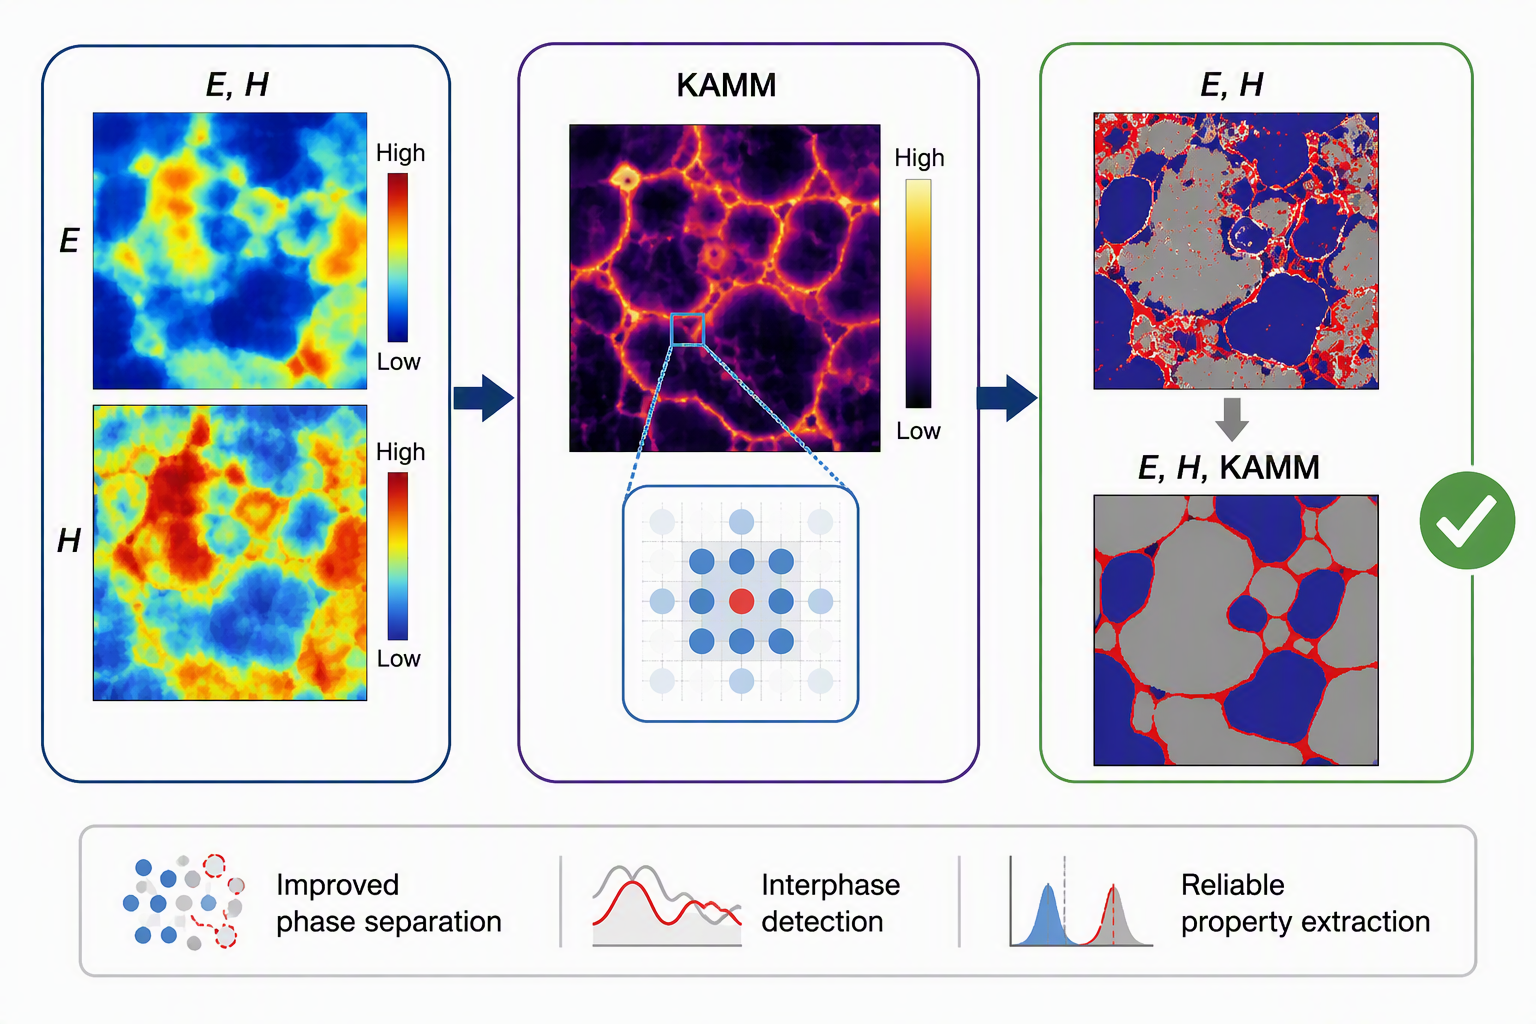
\includegraphics[width=\linewidth]{pictures/GraphicalAbstract.png}
\end{center}

% ----------------------------------------------------------
% Keywords (Elsevier format)
% ----------------------------------------------------------
\begin{keyword}
Nanomechanical Property Maps \sep Clustering \sep Multiphase materials \sep Kernel-Averaged Mechanical Mismatch (KAMM) \sep Neighborhood-based descriptors \sep Phase map \sep Modelling workflow
\end{keyword}

\end{frontmatter}

% ----------------------------------------------------------
% 1. Introduction
% ----------------------------------------------------------
\section{Introduction}

High-speed nanoindentation mapping has become a widely adopted technique for characterizing the local mechanical behavior of heterogeneous materials. By enabling the acquisition of neighborhood-resolved maps of hardness and elastic modulus, it provides a powerful means to investigate complex microstructures in metals and alloys, metallic glasses, composites, concretes, stones, and other multiphase systems~\cite{de_vasconcelos_grid_2016, kossman_mechanical_2019, nohazic_coating_2021, liang_spatial_2022, shi_determining_2023, dhal_mapping_2023, guo_machine_2025, chen_curve_2024, rossi_revealing_2025}. In parallel, atomic force microscopy (AFM)--based nanomechanical mapping has emerged as a complementary approach, offering higher spatial resolution and the ability to probe compliant or delicate surfaces with limited permanent deformation~\cite{randall_nanoindentation_2009, coq_germanicus_quantitative_2020, he_atomic_2018, garcia_advances_2025}. Together, these techniques enable high-throughput mechanical characterization at the submicron scale, bridging local mechanical responses with mesoscale microstructural features ~\cite{Miracle2021, Gianola2023}.
Beyond microstructure-focused analyses, extensive research has also been devoted to the mechanical behavior of nanostructured and nanocrystalline materials across a wide range of fields, further emphasizing the broad applicability of spatially resolved techniques such as nanoindentation and nanoscratch testing.

The growing availability of large-scale nanomechanical maps has driven the adoption of data-driven analysis methods. In particular, unsupervised machine learning approaches-most notably clustering algorithms-have been increasingly employed to automatically segment material domains exhibiting distinct mechanical behavior~\cite{mercier_tridimap_2018, mercier_microstructural_2019, bernachy-barbe_data_2019, chen_clustering_2021, giolando_ai-dente_2023, jentner_unsupervised_2023, zhang_unsupervised_2024}. When constituent phases display well-separated hardness (H) and elastic modulus (E) values, clustering based on these two features is generally effective. However, many heterogeneous materials exhibit overlapping mechanical responses due to similar phase stiffness, compositional gradients, or microstructural interactions. In such cases, clustering becomes ambiguous and may fail to reliably separate phases \cite{Constantinides2006, Ulm2019, alizade_comparative_2024}.

This segmentation is fundamentally governed by the underlying microstructure, as the spatial distribution, morphology, and interaction of phases directly influence the measured mechanical responses. Consequently, clustering results can be interpreted as a data-driven reconstruction of the microstructural organization, where each cluster corresponds to regions sharing similar mechanical signatures arising from their local structural environment.

These ambiguities are often associated with the presence of interfaces and interphases, which play a central role in governing the macroscopic behavior of composites and multiphase materials. Interfaces-sharp boundaries between discrete phases-can act as mechanical discontinuities or stress concentrators, potentially introducing measurement artefacts. Interphases-graded or diffuse transition regions-are frequently responsible for adhesion, damage tolerance, and transport properties~\cite{hausild_statistical_2019, hodzic_nano-indentation_2000, hausild_determination_2016}. Despite their importance, interfaces and interphases remain difficult to resolve experimentally. Their spatial extent may lie below the resolution limits of conventional microscopy, while their mechanical signatures can be masked by measurement noise, sampling artefacts, or insufficient contrast in H and E. As a result, interphase data points may be misclassified by clustering algorithms as belonging to adjacent phases or grouped into ambiguous intermediate clusters, thereby biasing phase identification and phase-specific property extraction~\cite{mercier_microstructural_2019, konstantopoulos_classification_2020, alizade_comparative_2024, ortizmembrado_2025}

To address these challenges, several strategies have been proposed. On the algorithmic side, alternative clustering methods and comparative benchmarking of clustering techniques have been explored to improve robustness in the presence of overlapping phase properties~\cite{alizade_comparative_2024}. On the feature level, additional descriptors beyond H and E have been introduced, including the H/E ratio, energy dissipation, indentation curve shape parameters, and machine-learning-derived features~\cite{jakes_nanoindentation_2009, lu_extraction_2020, kossman_pop-identification_2021, besharatloo_influence_2021, park_deep_2023, trost_explainable_2025}. Improved discrimination has also been achieved by correlating nanoindentation data with complementary characterization techniques, such as EBSD in metallic systems~\cite{bruno_advanced_2024}, or by performing indentation at multiple depths to probe subsurface heterogeneity~\cite{konstantopoulos_classification_2020}. More recently, physics-informed synthetic nanoindentation datasets have been proposed to systematically reproduce measurement variability, uncertainty, and artefacts, providing a traceable framework for controlled investigations of phase discrimination limits and the validation of data analysis and classification methodologies~\cite{maculotti_synthetic_2025}.

Despite these advances, many existing approaches remain constrained by the absence of explicit consideration of the spatial relationships between neighboring measurement points, which becomes essential when phase boundaries are diffuse or mechanically subtle. Without accounting for how adjacent data points are arranged and interact locally, clustering algorithms may fail to distinguish gradual transitions from true phase regions. This shortcoming hampers the robust identification of interfaces and interphases in complex material systems, thereby motivating the development of methodologies that integrate neighborhood-informed information, uncertainty quantification, and physics-informed data representations~\cite{puchi-cabrera_machine_2023}. In heterogeneous materials, neighborhood-based descriptors—including phase topology, morphology, size distributions, interfacial characteristics, spatial correlations, and orientation distributions—play a decisive role in determining the effective macroscopic properties. Whether the system consists of fibers, particles, grains, pores, or multiphase domains, neglecting the spatial arrangement of mechanical properties can lead to significant errors in property prediction and model calibration. Such frameworks enable the generation of realistic microstructural, RVE-based simulations that faithfully capture both morphological and mechanical heterogeneity~\cite{breuer_rve_2020, pardoen_nanomechanics_2021}.

In this work, we introduce and evaluate a neighborhood-informed mechanical descriptor, termed \textit{Kernel-Averaged Mechanical Mismatch} (KAMM), adapted from neighborhood metrics widely used in EBSD analysis~\cite{parish_cluster_2022,mtex_kam}. Rather than proposing a new clustering algorithm, the objective is to assess whether a simple, physically interpretable, and computationally efficient neighborhood descriptor can support phase discrimination and the identification of local mechanical heterogeneity in nanomechanical property maps. KAMM quantifies local mechanical heterogeneity by measuring the deviation of a given measurement point from its surrounding neighborhood in the $(E,H)$ space. High KAMM values are generally associated with interfaces, interphases, or regions exhibiting strong local mechanical gradients, whereas low values indicate locally homogeneous mechanical behavior. By extending the clustering space to $(E,H,\mathrm{KAMM})$, spatial context can be incorporated into otherwise feature-based clustering workflows. The proposed framework is evaluated through a two-stage validation strategy. First, controlled synthetic datasets with known phase distributions are used to systematically assess clustering performance under varying levels of mechanical contrast, interphase thickness, microstructural complexity, and noise. Second, the approach is applied to an experimental nanoindentation dataset from the literature to examine its practical behavior under experimental conditions where pixel-level ground-truth labels are unavailable. KAMM belongs to a broader family of spatially informed descriptors, including local gradient measures, statistical neighborhood descriptors, graph-based representations, and spatially constrained clustering approaches. The aim of this study is not to provide an exhaustive comparison with all such methods, but rather to determine whether a simple mismatch-based descriptor can deliver practical benefits for nanomechanical phase mapping. A comprehensive comparison with alternative spatial descriptors remains an important direction for future work.

Controlled synthetic datasets with known phase labels provide a rigorous basis for quantifying clustering performance and assessing the contribution of neighborhood information. The results show that KAMM can improve phase recovery for selected clustering algorithms and microstructural configurations, while other combinations show limited benefit or degraded performance. The observed benefits are therefore algorithm- and dataset-dependent, highlighting both the potential and the limitations of neighborhood-informed descriptors for nanomechanical phase mapping.

The structure of the paper is as follows. Section~\ref{sec:methods} presents the proposed methodology, including the generation of synthetic benchmark microstructures, the clustering strategies considered, and the formulation of the KAMM descriptor. Section~\ref{sec:results} first quantifies the impact of KAMM on synthetic datasets with varying levels of mechanical contrast, interphase thickness, and microstructural complexity, and subsequently evaluates its applicability to experimental nanoindentation datasets from the literature. Finally, Section~\ref{sec:conclusion} summarizes the main findings, discusses the strengths and limitations of the proposed framework, and outlines directions for future research.

% ----------------------------------------------------------
% 2. Materials and Methods
% ----------------------------------------------------------
\section{Materials and Methods}
\label{sec:methods}

\subsection{Synthetic Specimen Generation}
\label{sec:synthetic_specimens}

\paragraph{Rationale and benchmarking challenge}

A central difficulty in evaluating clustering algorithms for nanomechanical phase identification lies in the absence of ground truth for experimental datasets. Real materials exhibit unknown phase labels, uncontrolled noise sources, spatial correlations, and scale-dependent interactions, making quantitative benchmarking inherently ambiguous. Conversely, overly simplistic synthetic datasets (e.g., perfectly separable Gaussian clusters without spatial structure) lead to artificially optimistic clustering performance and fail to represent the complexity of multiphase microstructures.

Constructing a meaningful synthetic benchmark therefore requires balancing three competing constraints:
(i) exact knowledge of phase labels,
(ii) tunable mechanical contrast and noise levels,
and (iii) realistic spatial organization, including sharp interfaces, diffuse transitions, curvature effects, and non-compact morphologies.

To address this, we developed a fully parametric Python-based generation framework that programmatically constructs synthetic nanomechanical maps under controlled and reproducible conditions. The script defines the spatial grid, assigns phase geometries, imposes user-defined mechanical contrast via $(E_\mathrm{ratio}, H_\mathrm{ratio})$, and injects configurable intra-phase Gaussian noise and optional property gradients. All geometric parameters (e.g., inclusion size, interphase width, particle distribution, curvature), mechanical ratios, and noise levels are explicitly tunable, enabling systematic exploration of clustering performance across a wide range of controlled scenarios.

Using this framework, we generated four families of synthetic nanomechanical datasets that emulate representative microstructural patterns encountered in multiphase materials. Each dataset provides exact phase labels, user-defined mechanical contrast, controlled intra-phase variability, and optional neighborhood-level gradients. For every configuration, the generator automatically exports:
\begin{itemize}
    \item a synthetic indentation dataset ($H$, $E$ per pixel),
    \item the corresponding ground-truth phase map (image and CSV),
    \item configuration metadata (all input parameters),
    \item and phase-level summary statistics.
\end{itemize}

It is assumed that the spatial resolution is sufficient for each indentation test (i.e., each synthetic pixel) to probe a single phase. This requires appropriate scale separation: the maximum indentation depth is kept smaller than the characteristic microstructural length scale (e.g., $h_\text{max} \lesssim 0.1D$, with $D$ the mean particle diameter or interphase width), while remaining larger than the surface roughness (e.g., $h_\text{max} > 3R_q$). In addition, the indentation spacing $d$ is chosen larger than approximately twice the plastic zone radius to prevent interaction between adjacent indents. Under these conditions, each measurement reflects intrinsic phase properties rather than composite or roughness-affected responses~\cite{randall_nanoindentation_2009}. The synthetic framework nevertheless remains an idealized two-dimensional representation. Each synthetic pixel is assigned a single local mechanical response, including near phase boundaries. Consequently, the model does not explicitly reproduce the mixed response that may arise when the mechanically affected volume of an indentation intersects more than one phase. The Gaussian intra-phase variability and prescribed property gradients represent measurement dispersion and idealized spatial transitions, respectively, rather than a mechanical model of phase mixing beneath the indenter. Moreover, the two-dimensional maps do not account for subsurface heterogeneity or three-dimensional phase geometry. The synthetic benchmarks are therefore intended to evaluate clustering behavior under controlled conditions rather than to reproduce the complete indentation response of a heterogeneous material. Rather than creating trivially separable clusters, the objective of these datasets is to systematically probe clustering robustness under: 
\begin{itemize} \item low to high mechanical contrast, \item overlapping property distributions, \item sharp versus graded interfaces, \item curved versus planar boundaries, \item and diffuse, spatially ambiguous morphologies. 
\end{itemize}

The use of Gaussian intra-phase variability is also a simplifying assumption. Experimental nanoindentation property distributions may exhibit non-Gaussian behavior, including asymmetric, heavy-tailed, or multimodal distributions, as well as outliers or heteroscedastic variability. Consequently, the noise-robustness results presented here should be interpreted specifically within the context of Gaussian perturbations and should not be generalized to arbitrary experimental property distributions. More flexible or empirically derived distributions could be incorporated in future extensions of the synthetic framework.

\paragraph{Five-region quadrant + center system (feature exploration)}

This benchmark divides the grid into four quadrants with distinct mechanical properties and a central compliant inclusion (Fig.~\ref{fig:five_region_example}). The assigned phase properties span a broad range (from $H\!\approx\!0.2$~GPa up to $H\!\approx\!5$~GPa and from $E\!\approx\!10$--$50$~GPa), enabling exploration of low-, moderate-, and high-contrast configurations through the implied ratios $(E_\mathrm{ratio},H_\mathrm{ratio})$.

Gaussian noise is added within each region (typically $\sigma_H=0.1$~GPa and $\sigma_E=0.2$~GPa), introducing intra-phase dispersion and partial overlap between clusters. Because geometry is fixed and certain phase pairs may exhibit subtle contrast, this dataset is primarily intended for feature-behavior analysis rather than pure clustering validation. It enables controlled comparison of scalar descriptors ($H$, $E$, $H/E$, $H^3/E^2$) and neighborhood-based descriptors (e.g., KAMM-based features), particularly near boundaries and in regions of moderate contrast.

\begin{figure}[htbp]
\centering
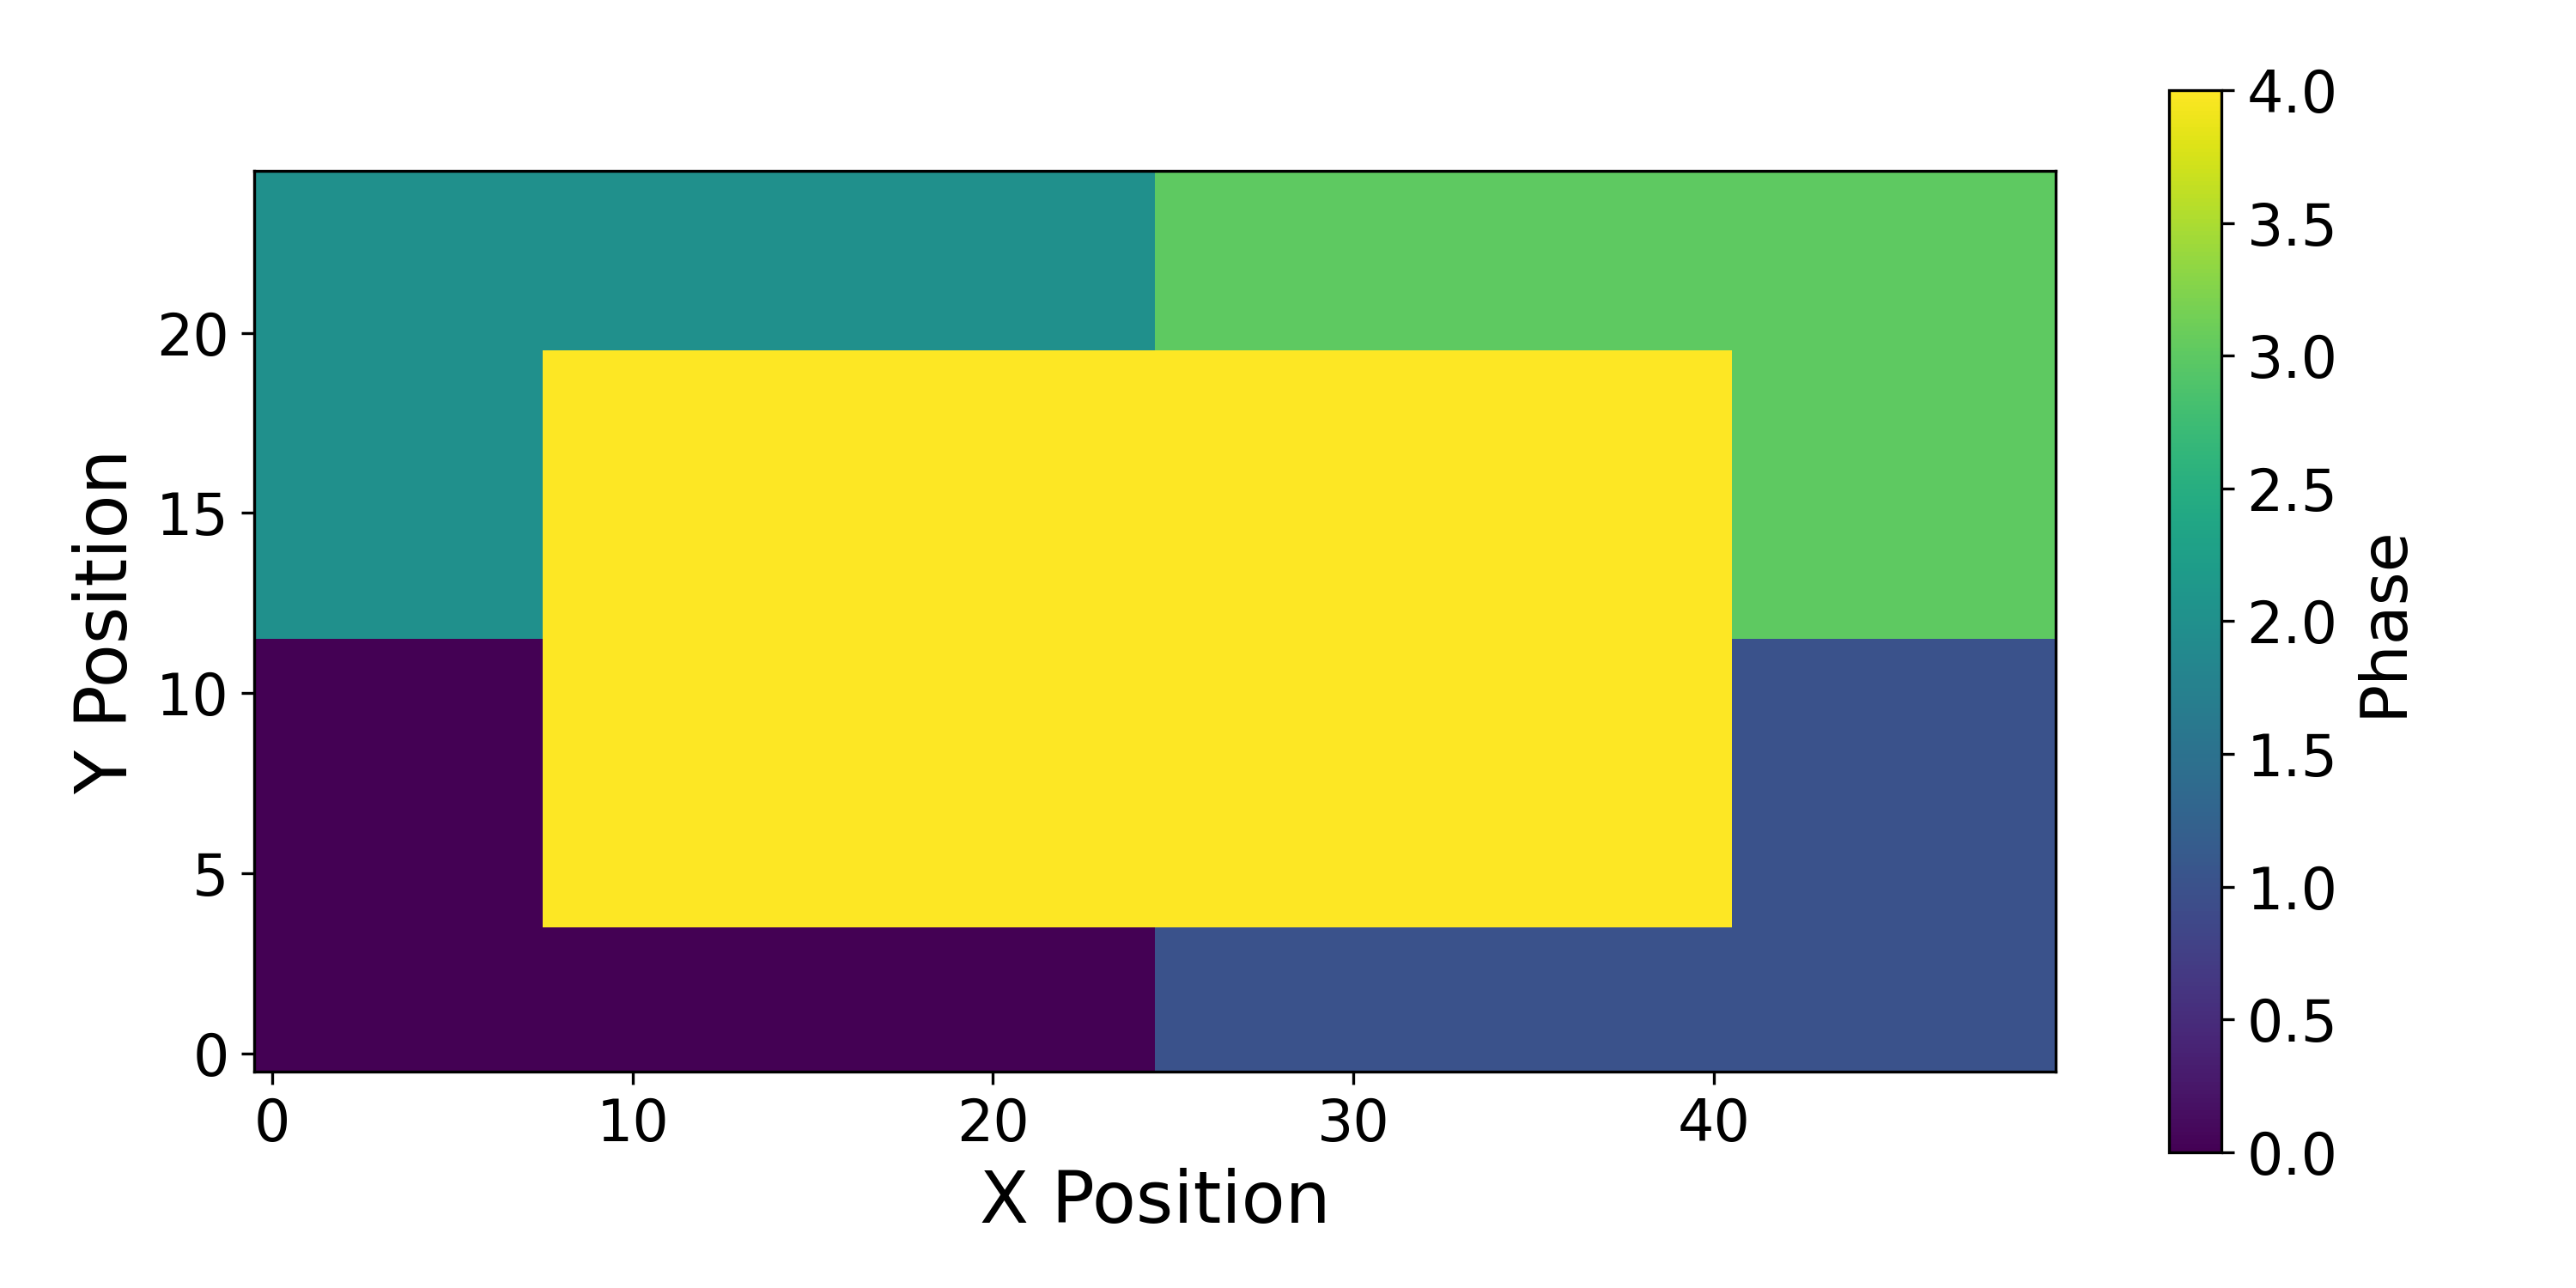
\includegraphics[width=0.65\columnwidth]{pictures/phase_map_5regions.png}
\caption{Five-region specimen used to illustrate sensitivity of scalar and neighborhood-based descriptors.}
\label{fig:five_region_example}
\end{figure}

\paragraph{Rectangular composite with sharp or graded interface}

This one-dimensional configuration consists of a matrix (left), a fiber phase (right), and an optional interphase region (Fig.~\ref{fig:synthetic_examples}(a--c)). When the interphase width is zero, the system reduces to a sharp two-phase composite (Fig.~\ref{fig:synthetic_examples}(a)). Nonzero widths introduce a graded transition in which $H$ and $E$ vary smoothly across the interface (Fig.~\ref{fig:synthetic_examples}(b,c)). Relative interphase widths of 0.03 and 0.05 were used to simulate realistic gradients. Mechanical contrast is controlled via $(E_\mathrm{ratio}, H_\mathrm{ratio})$, while low-amplitude Gaussian noise is added within each region (typically $\sigma_H = 0.1$~GPa and $\sigma_E = 0.1$~GPa) to emulate experimental variability. Despite its simple geometry, this configuration is non-trivial from a clustering standpoint: graded interfaces blur phase boundaries, reduce cluster separability in feature space, and introduce spatial correlation. It therefore provides a controlled framework for evaluating sensitivity to diffuse transitions and boundary localization accuracy.

\paragraph{Matrix--fiber composite with optional annular interphase}

This dataset simulates a periodic fiber-reinforced composite with circular inclusions arranged on a regular grid (Fig.~\ref{fig:synthetic_examples}(d,e)). An interphase layer of user-defined thickness may surround each fiber, resulting in either a two-phase (matrix/fiber) configuration (Fig.~\ref{fig:synthetic_examples}(d)) or a three-phase (matrix/interphase/fiber) system (Fig.~\ref{fig:synthetic_examples}(e)).

Mechanical properties are sampled from Gaussian clusters whose means are defined by $(E_\mathrm{ratio}, H_\mathrm{ratio})$. Curved boundaries and concentric gradients introduce classification ambiguity near interfaces, particularly when contrast is low. This configuration challenges clustering methods in the presence of non-planar geometry and radially varying properties.

\paragraph{Matrix--particle composite with diffuse random particles}

This two-phase system consists of a homogeneous matrix embedding soft, irregular inclusions generated by superposition of Gaussian peaks at random positions (Fig.~\ref{fig:synthetic_examples}(f)). Unlike the fiber case, morphology is neither periodic nor sharply defined.

The resulting diffuse transitions mimic poorly resolved or chemically graded particle boundaries. Since geometry is not explicitly prescribed, particle regions are inferred by thresholding the hardness field. This dataset is intentionally challenging: clusters may be non-compact in feature space, spatially irregular, and partially overlapping. It probes algorithm robustness under low contrast, random morphology, and spatial ambiguity.

\paragraph{Mechanical parameterization and contrast scaling}

The mechanical properties assigned to the synthetic geometries described above are defined per pixel (except for the five-region feature-exploration case, which uses fixed values). For the composite configurations (rectangular, matrix--fiber, and matrix--particle), mechanical contrast is introduced systematically via scaling ratios:

\[
E_\mathrm{ratio},\, H_\mathrm{ratio} \in [1.0,\,3.0],
\]

with selected high-contrast cases extending to 5 or 10 for the matrix--particle configuration (see Fig.~\ref{fig:synthetic_examples}(f)).

The lower bound ($\approx 1$) intentionally produces nearly indistinguishable phases, where clustering becomes ill-posed. Moderate ratios (2--3) correspond to common multiphase systems, whereas higher ratios represent extreme ceramic/metal or glass/polymer mismatches. This controlled variation enables systematic evaluation of clustering stability as a function of separability in mechanical feature space.

\begin{figure*}[htbp]
\centering

% --- Row 1 ---
\subfloat[Rectangular composite, sharp interface]{
    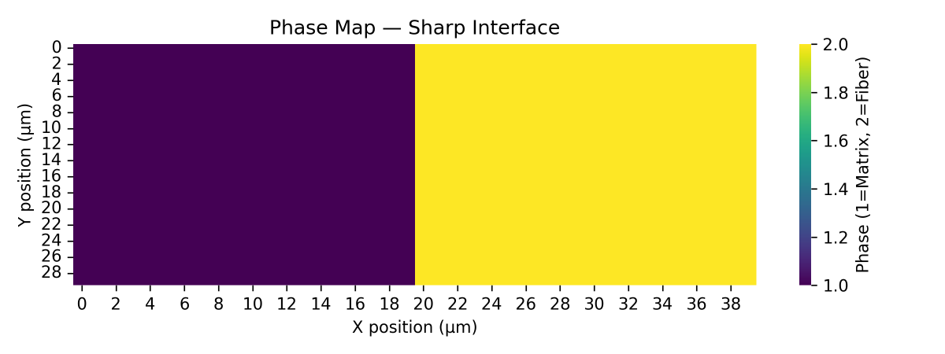
\includegraphics[width=0.32\textwidth]{pictures/Rect2PhasesSharp.png}
}
\hfill
\subfloat[Rectangular composite, small interphase]{
    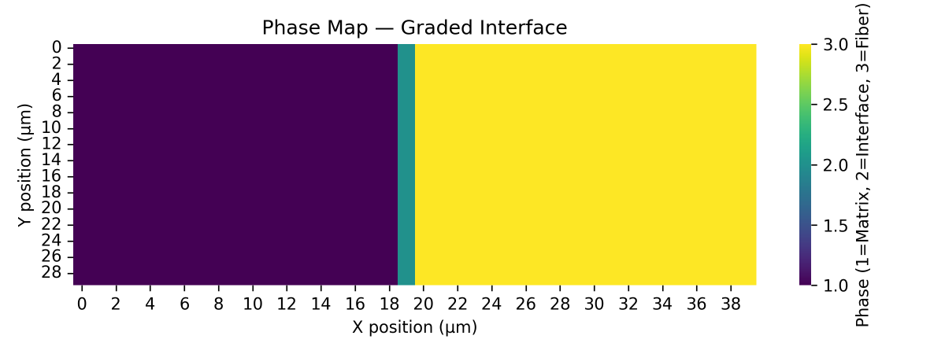
\includegraphics[width=0.32\textwidth]{pictures/Rect2PhasesSmallInterphase.png}
}
\hfill
\subfloat[Rectangular composite, large interphase]{
    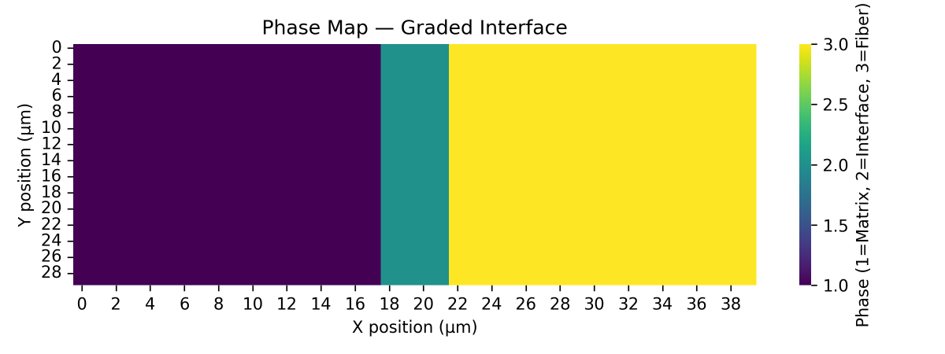
\includegraphics[width=0.32\textwidth]{pictures/Rect2PhasesLargeInterphase.png}
}

\vspace{0.6em}

% --- Row 2 ---
\subfloat[Matrix--fiber composite (no interphase)]{
    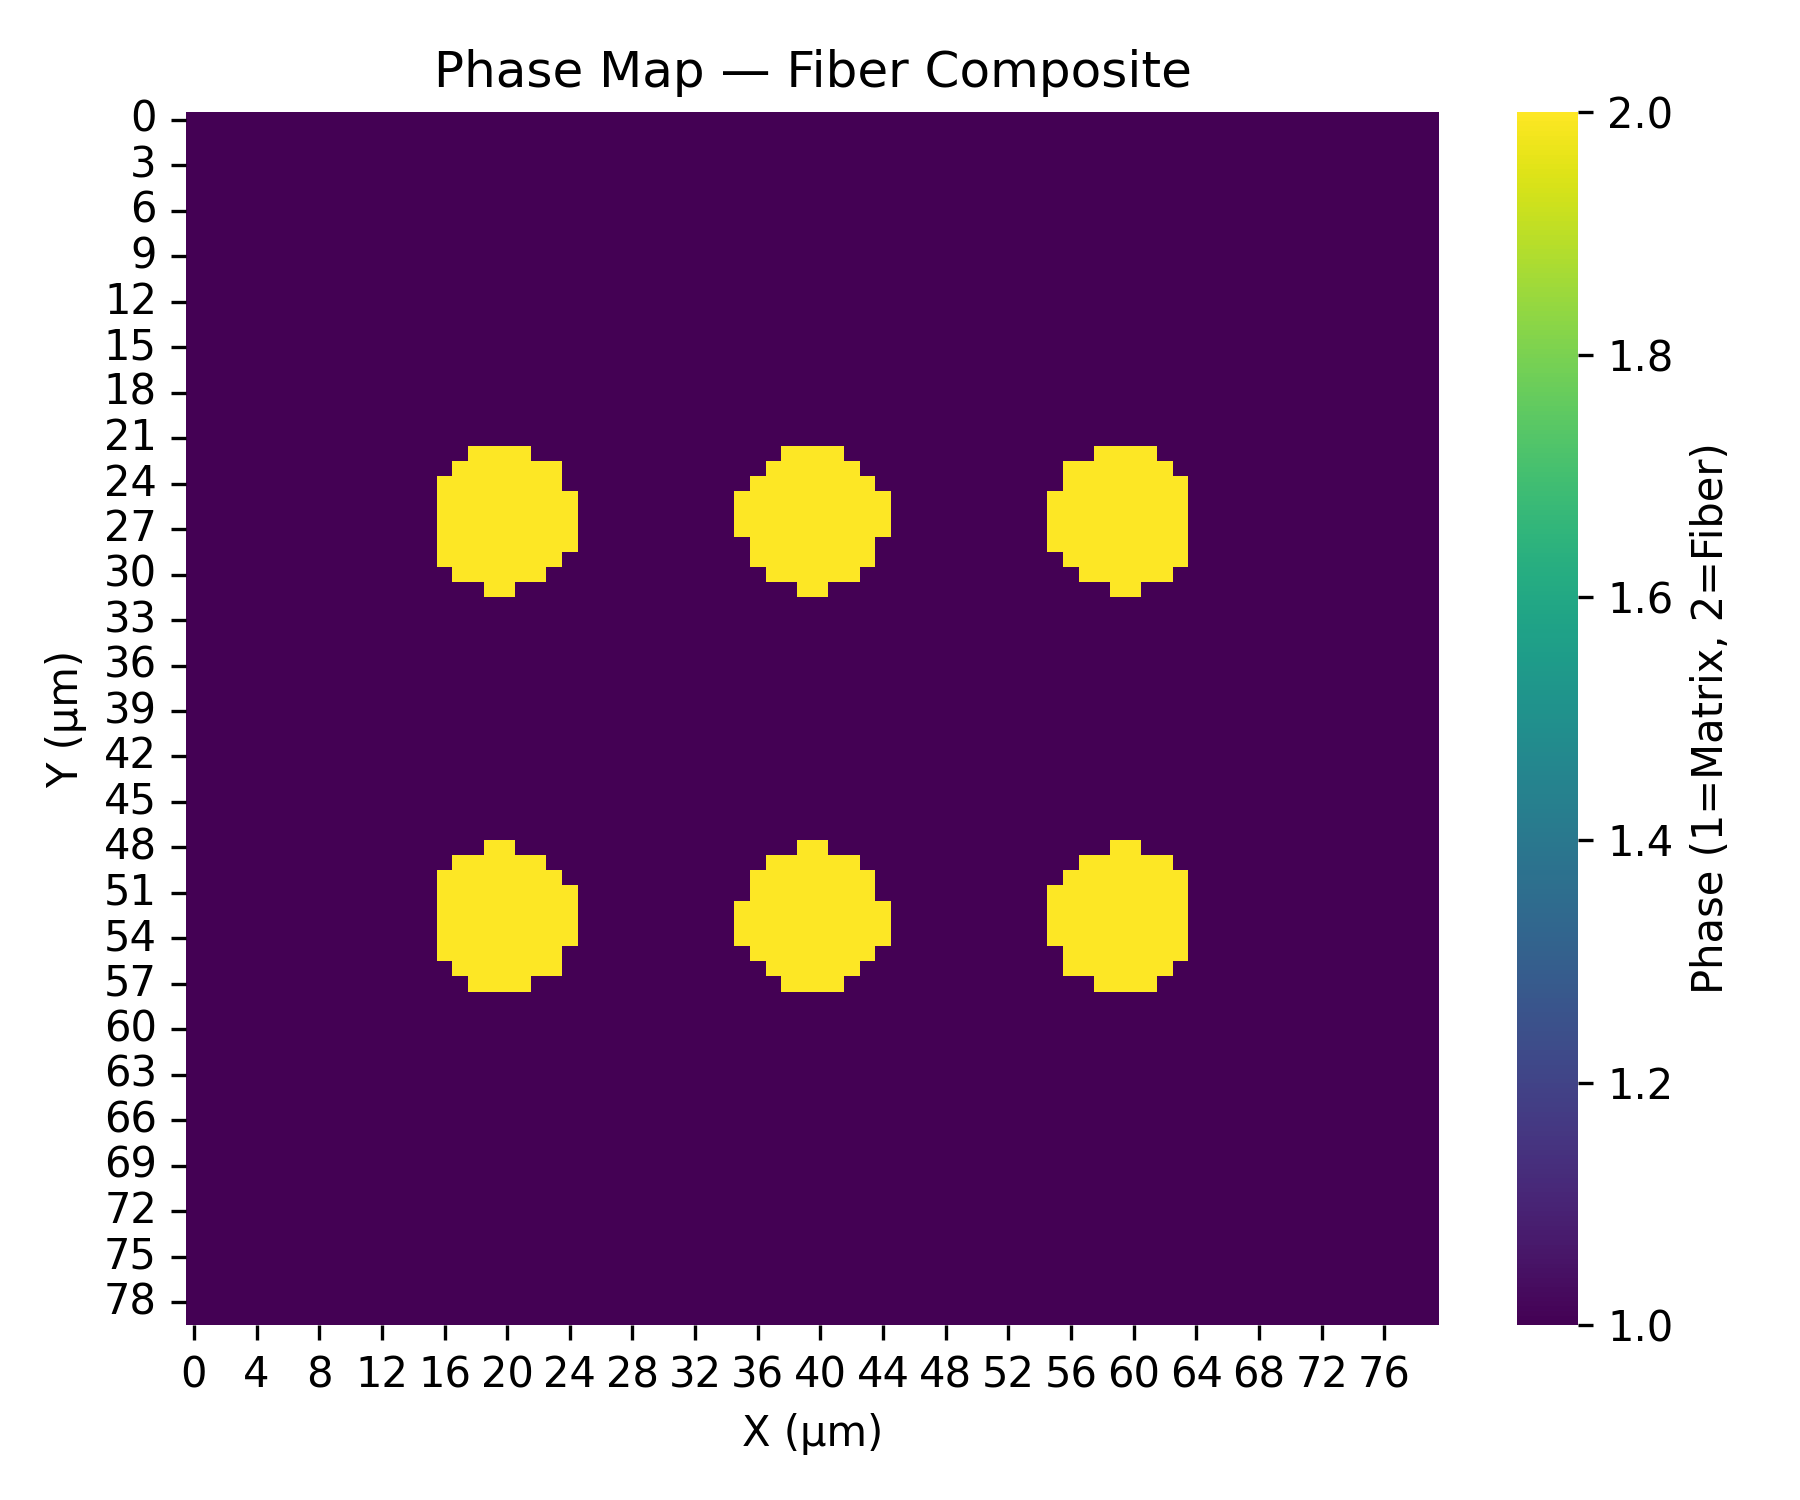
\includegraphics[width=0.32\textwidth]{pictures/MatrixFibersNoInterphase.png}
}
\hfill
\subfloat[Matrix--fiber composite (with annular interphase)]{
    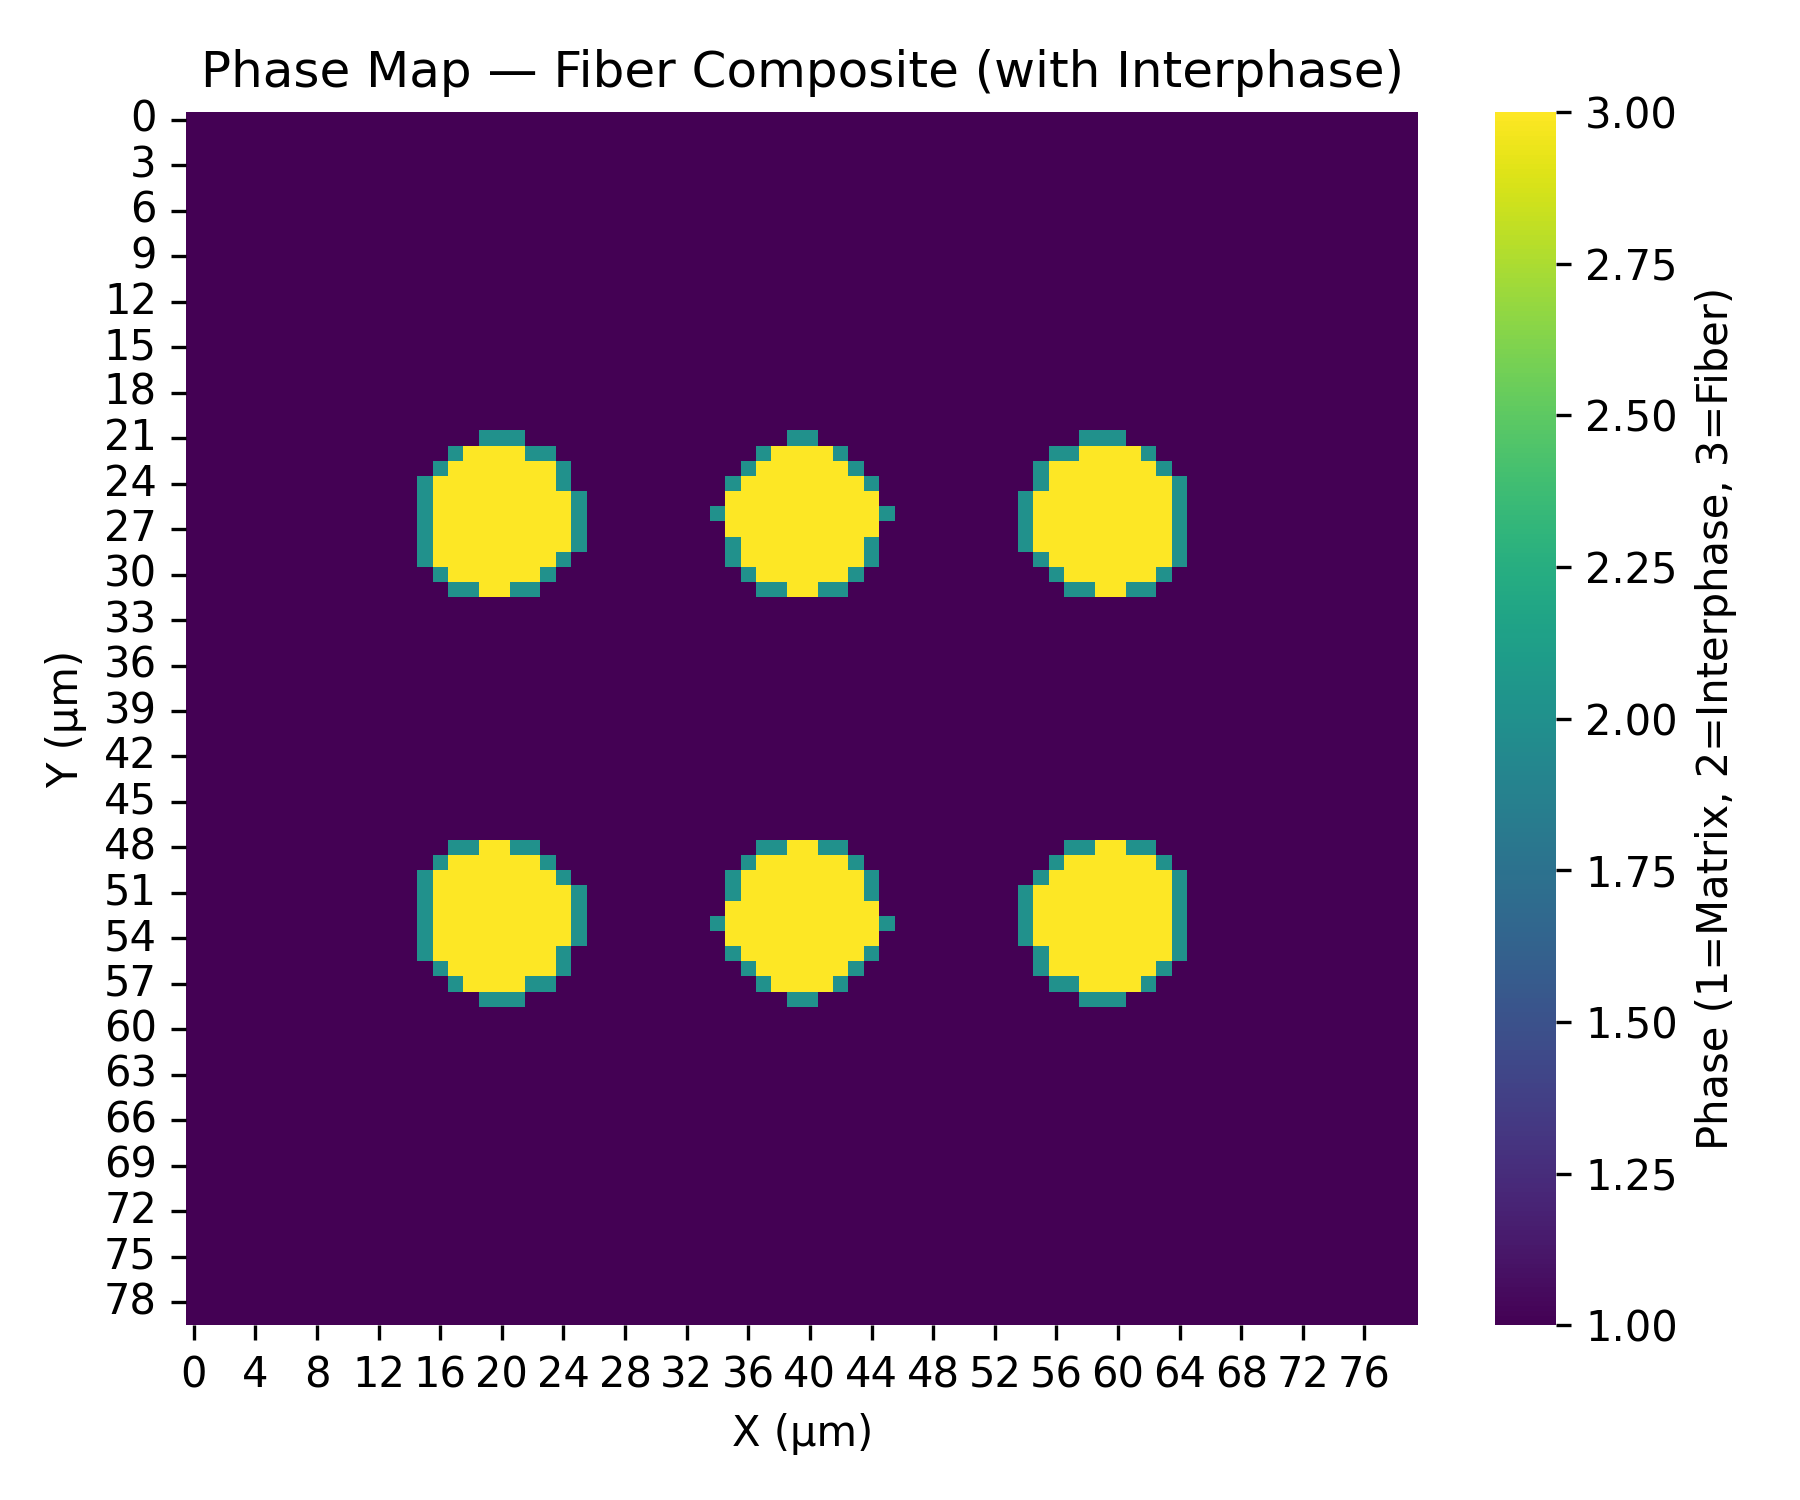
\includegraphics[width=0.32\textwidth]{pictures/MatrixFibersInterphase.png}
}
\hfill
\subfloat[Matrix--particle composite with diffuse inclusions]{
    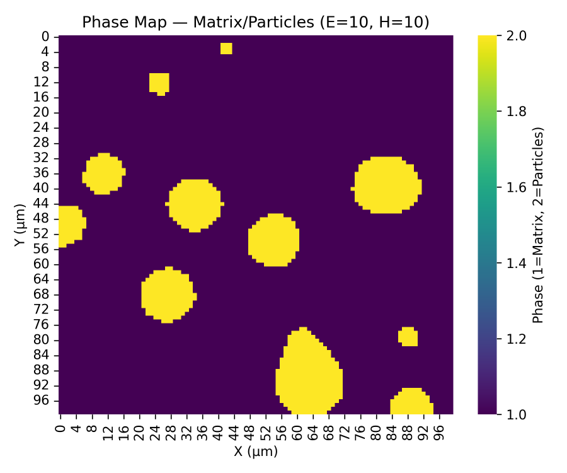
\includegraphics[width=0.32\textwidth]{pictures/MatrixParticles.png}
}

\caption{Synthetic specimen families used for benchmarking clustering performance. 
The configurations span sharp and graded planar interfaces (a--c), periodic circular inclusions with and without interphase layers (d--e), and diffuse, randomly distributed particles (f). 
Together, these geometries provide controlled yet structurally diverse scenarios for evaluating clustering robustness under varying mechanical contrast and morphological complexity.}
\label{fig:synthetic_examples}
\end{figure*}

Figure~\ref{fig:synthetic_examples} summarizes the synthetic specimen families, highlighting the diversity of spatial structures---sharp, graded, circular, and diffuse---used to construct a benchmark that is controlled yet sufficiently complex to avoid trivial clustering scenarios.

\paragraph{Experimental validation}

To assess practical relevance beyond controlled synthetic conditions, the clustering framework was also applied to experimental nanomechanical data from a nickel--silicon carbide (Ni--SiC) composite coating reported in~\cite{mercier_microstructural_2019}. This system features hard ceramic inclusions dispersed within a metallic matrix and provides a realistic test case where phase labels are not explicitly known, allowing qualitative comparison with microstructural observations.

\subsection{KAMM features and clustering pipeline}
\label{sec:kamm_method}

This subsection introduces the neighborhood-based mechanical descriptors and the clustering framework used for phase identification. In particular, we define the \textbf{Kernel-Averaged Mechanical Mismatch (KAMM)}, inspired by the \textit{Kernel Average Misorientation (KAM)} metric used in EBSD. By quantifying local mechanical heterogeneity through comparisons of each indentation point's $(E,H)$ values with those of its neighbors, KAMM is intended to provide boundary-sensitive spatial information that may support phase separability under limited mechanical contrast.

\begin{figure}[htbp]
\centering
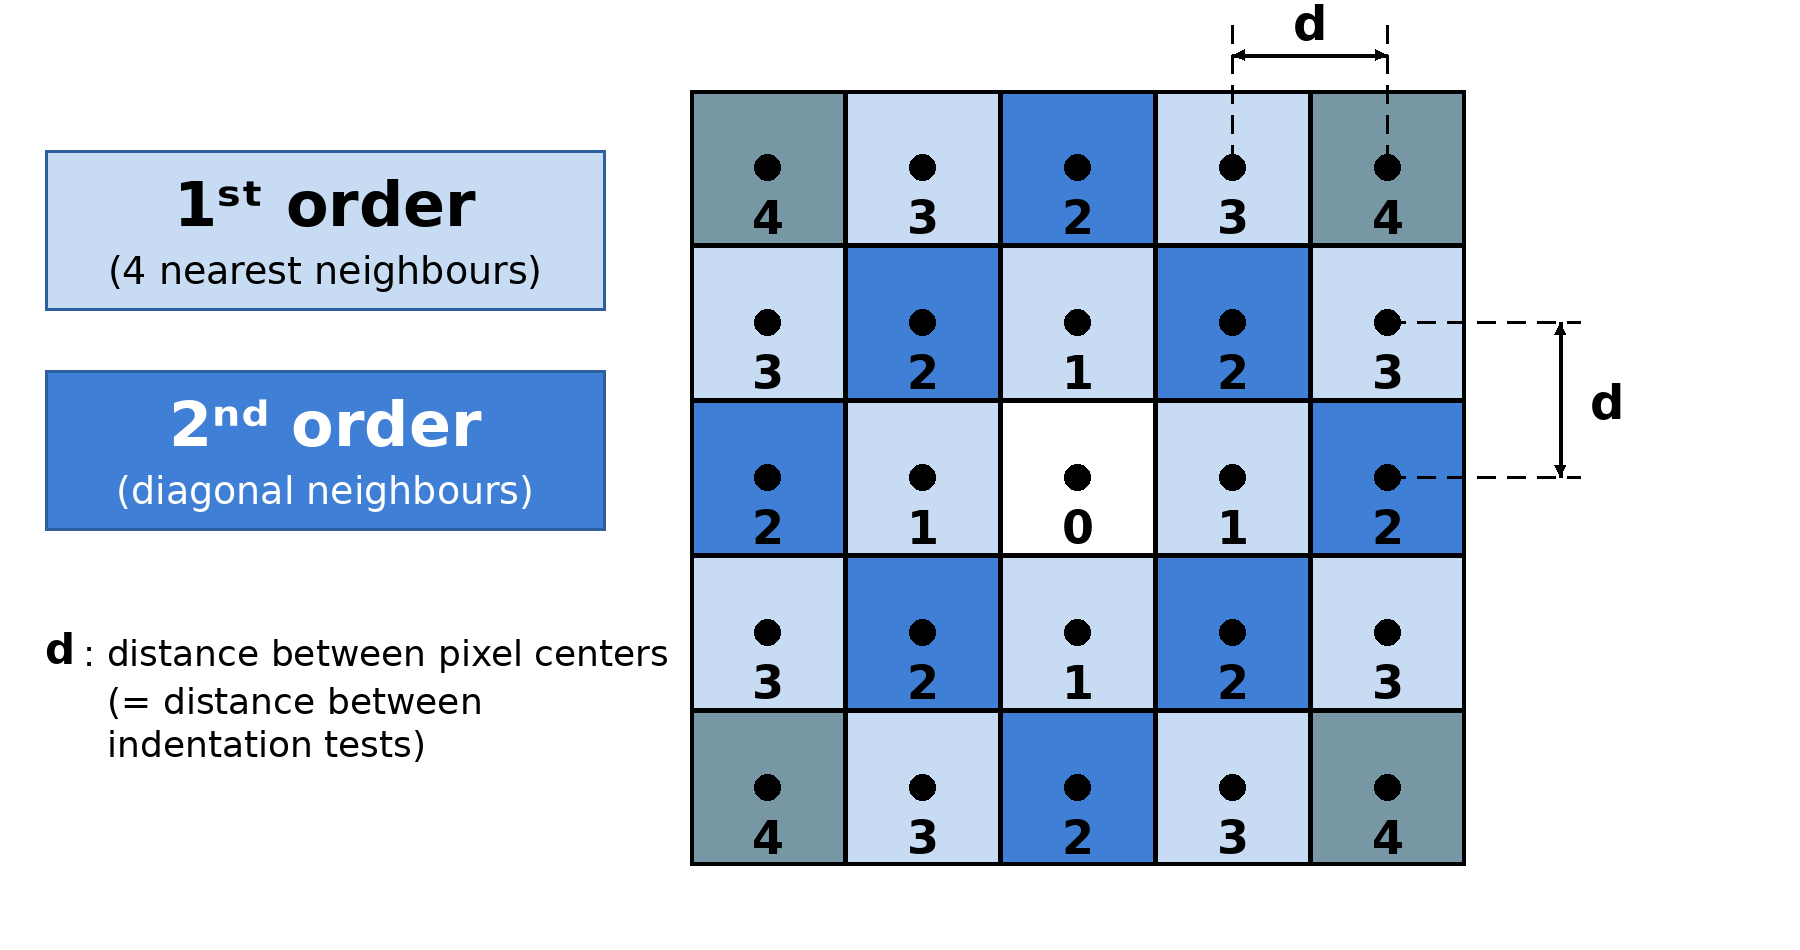
\includegraphics[width=0.65\columnwidth]{pictures/KAMM_orders.png}
\caption{Pixel connectivity schemes used for KAMM, with first-order neighborhood (4 nearest neighbors in light blue) and second-order neighborhood (includes diagonals and two-pixel offsets in dark blue).}
\label{fig:kam_neighbors}
\end{figure}

\paragraph{Standard KAMM}
For a point \(i\) with a neighbor set \(\mathcal{N}_i\) of size \(N_i\), the default KAMM metric is defined as the average absolute mismatch of the modulus--hardness product:
\begin{equation}
\label{eq:kamm}
\text{KAMM}_i
=
\frac{1}{N_i}
\sum_{k \in \mathcal{N}_i}
\bigl| E_i H_i - E_k H_k \bigr|.
\end{equation}

The modulus-hardness product was selected as a simple coupled mechanical indicator that increases when both stiffness and resistance to plastic deformation increase simultaneously. Unlike KAEM and KAPM, which isolate variations in a single property, KAMM combines both quantities into a single mismatch measure and therefore provides a compact description of local mechanical heterogeneity. The proposed formulation should not be interpreted as unique or optimal. The present definition evaluates mismatch using the modulus-hardness product as a coupled mechanical indicator. Alternative neighborhood descriptors could instead be formulated directly in the $(E,H)$ feature space using Euclidean or Mahalanobis distances, or through local variance, covariance, or gradient-based measures of mechanical heterogeneity. Evaluating the relative performance of such descriptors for nanomechanical phase mapping constitutes an interesting direction for future work.

\paragraph{Component-wise mismatch metrics}
Two scalar projections isolate the mismatch in each property:
\begin{align}
\label{eq:kaem}
\text{KAEM}_i &=
\frac{1}{N_i}
\sum_{k \in \mathcal{N}_i}
\lvert E_i - E_k \rvert,
\\[4pt]
\label{eq:kapm}
\text{KAPM}_i &=
\frac{1}{N_i}
\sum_{k \in \mathcal{N}_i}
\lvert H_i - H_k \rvert.
\end{align}

\paragraph{Alternative KAMM formulations}
Two additional formulations capture relative or coupled variations between modulus and hardness:
\begin{itemize}
    \item \textbf{KAMM\textsubscript{RATIO}:}
    \begin{equation}
    \text{KAMM}_{\mathrm{ratio},\,i}
    =
    \frac{1}{N_i}
    \sum_{k \in \mathcal{N}_i}
    \left\lvert
    \frac{E_i-E_k}{H_i-H_k+\varepsilon}
    \right\rvert,
    \end{equation}
    where $\varepsilon=10^{-6}$~GPa is a small positive regularization term introduced to reduce numerical instability when the local hardness difference approaches zero. Because $\varepsilon$ is added to the signed hardness difference, exceptionally small denominators may nevertheless occur when $H_i-H_k \approx -\varepsilon$.

    \item \textbf{KAMM\textsubscript{NORMPROD}:}
    \begin{equation}
    \text{KAMM}_{\mathrm{normprod},\,i}
    =
    \frac{1}{N_i}
    \sum_{k \in \mathcal{N}_i}
    \frac{(E_i-E_k)(H_i-H_k)}{\sigma_E\,\sigma_H},
    \end{equation}
    where $\sigma_E$ and $\sigma_H$ are the global standard deviations of $E$ and $H$, respectively.
\end{itemize}

Non-finite descriptor values may occur during feature calculation and appear as blank pixels in the corresponding maps. For KAMM\textsubscript{RATIO}, the regularization term $\varepsilon=10^{-6}$~GPa reduces numerical instability when $H_i-H_k$ approaches zero, although an exceptionally small denominator may still occur when $H_i-H_k \approx -\varepsilon$. For KAMM\textsubscript{NORMPROD}, non-finite values may arise from non-finite input values or from an undefined normalization if $\sigma_E$ or $\sigma_H$ is zero or non-finite. A locally homogeneous neighborhood does not by itself constitute a missing value. Before clustering, selected feature values are converted to numeric form. Non-finite or missing values are treated as missing and imputed using the mean of the corresponding feature; if no valid feature mean is available, a value of zero is used. The resulting complete feature matrix is then standardized using z-score scaling before clustering.

These variants emphasize relative or coupled mismatch and can highlight diffuse gradients or subtle transitions in the modulus--hardness fields.

\paragraph{Neighborhood connectivity}
KAMM is computed over spatial neighbors defined by the connectivity schemes illustrated in Fig.~\ref{fig:kam_neighbors}:
\begin{itemize}
    \item \textbf{First-order} ($\mathcal{O}_1$): 4-connectivity (up, down, left, right)
    \item \textbf{Second-order} ($\mathcal{O}_2$): includes diagonals and two-pixel offsets (up to 8 neighbors)
\end{itemize}

\begin{figure}[htbp]
\centering

% --- Row 1 ---
\begin{minipage}{0.45\linewidth}
    \subfloat[Hardness ($H$), units: GPa]{
        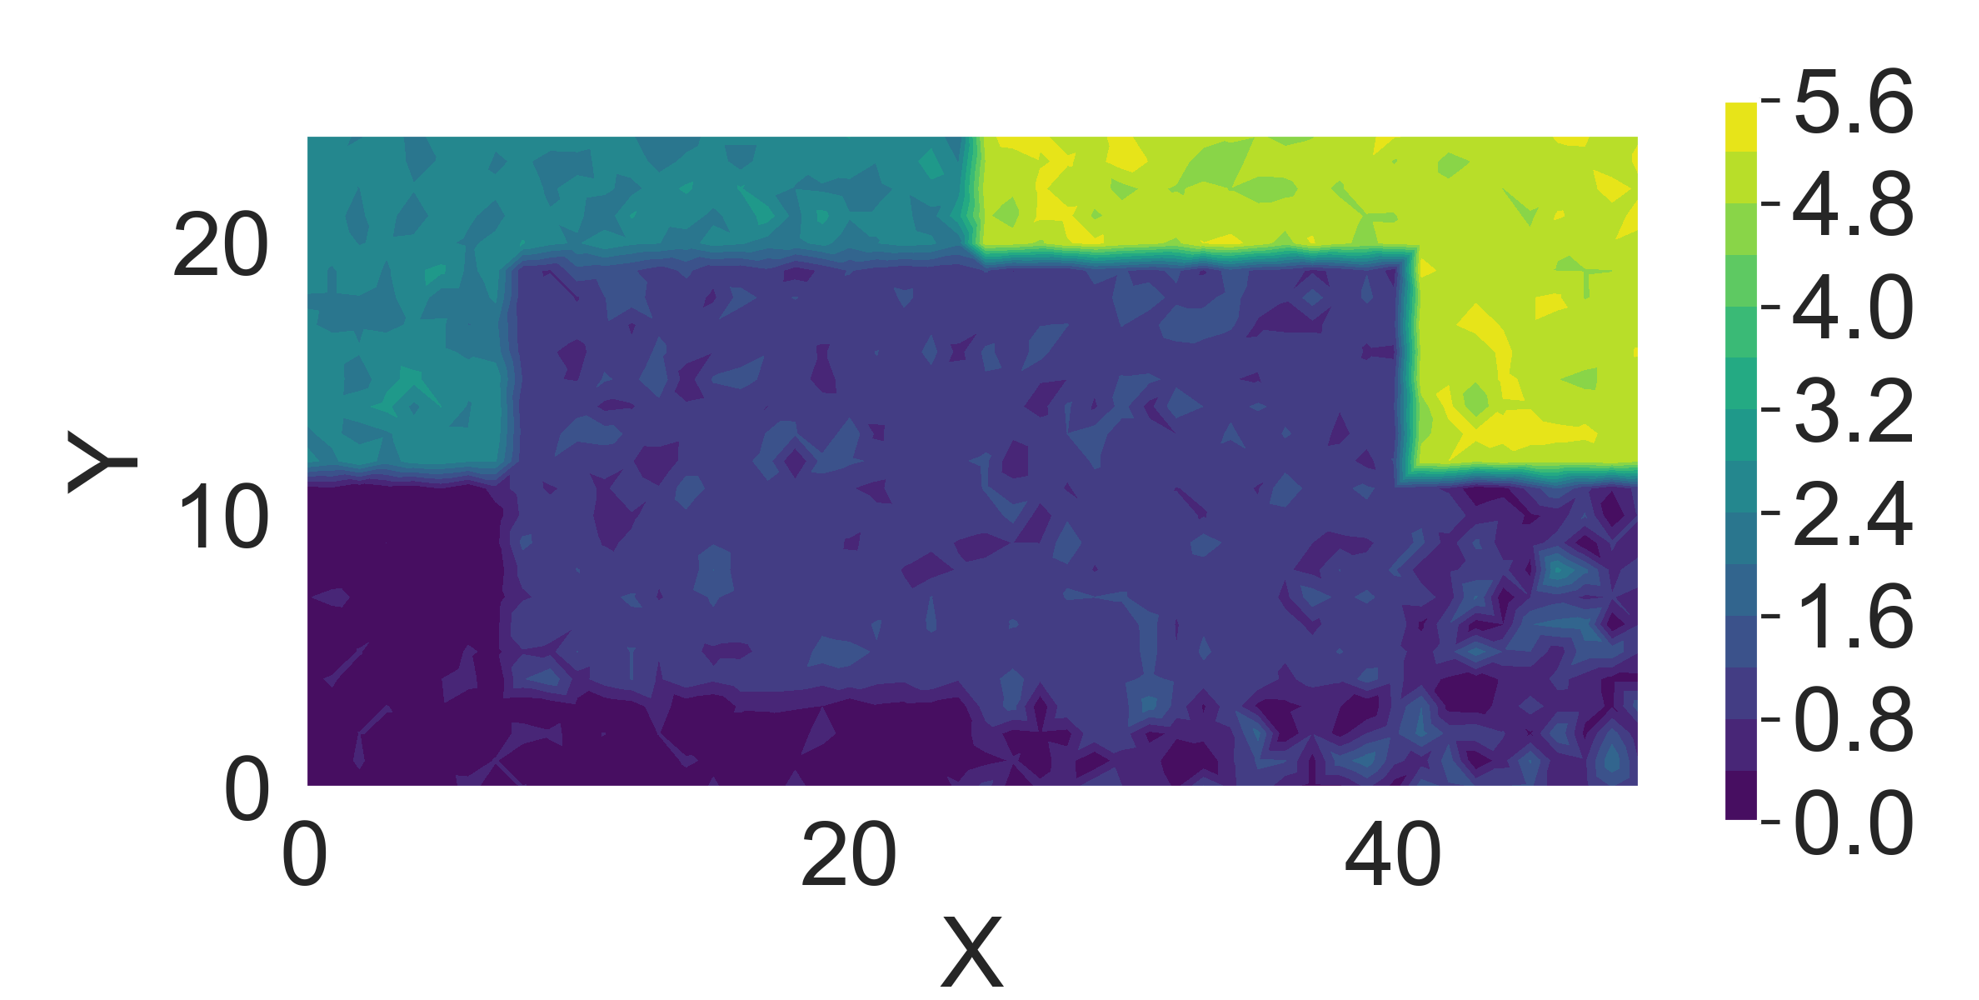
\includegraphics[width=0.9\linewidth]{pictures/H_map.png}
    }
\end{minipage}
\hfill
\begin{minipage}{0.45\linewidth}
    \subfloat[Modulus ($E$), units: GPa]{
        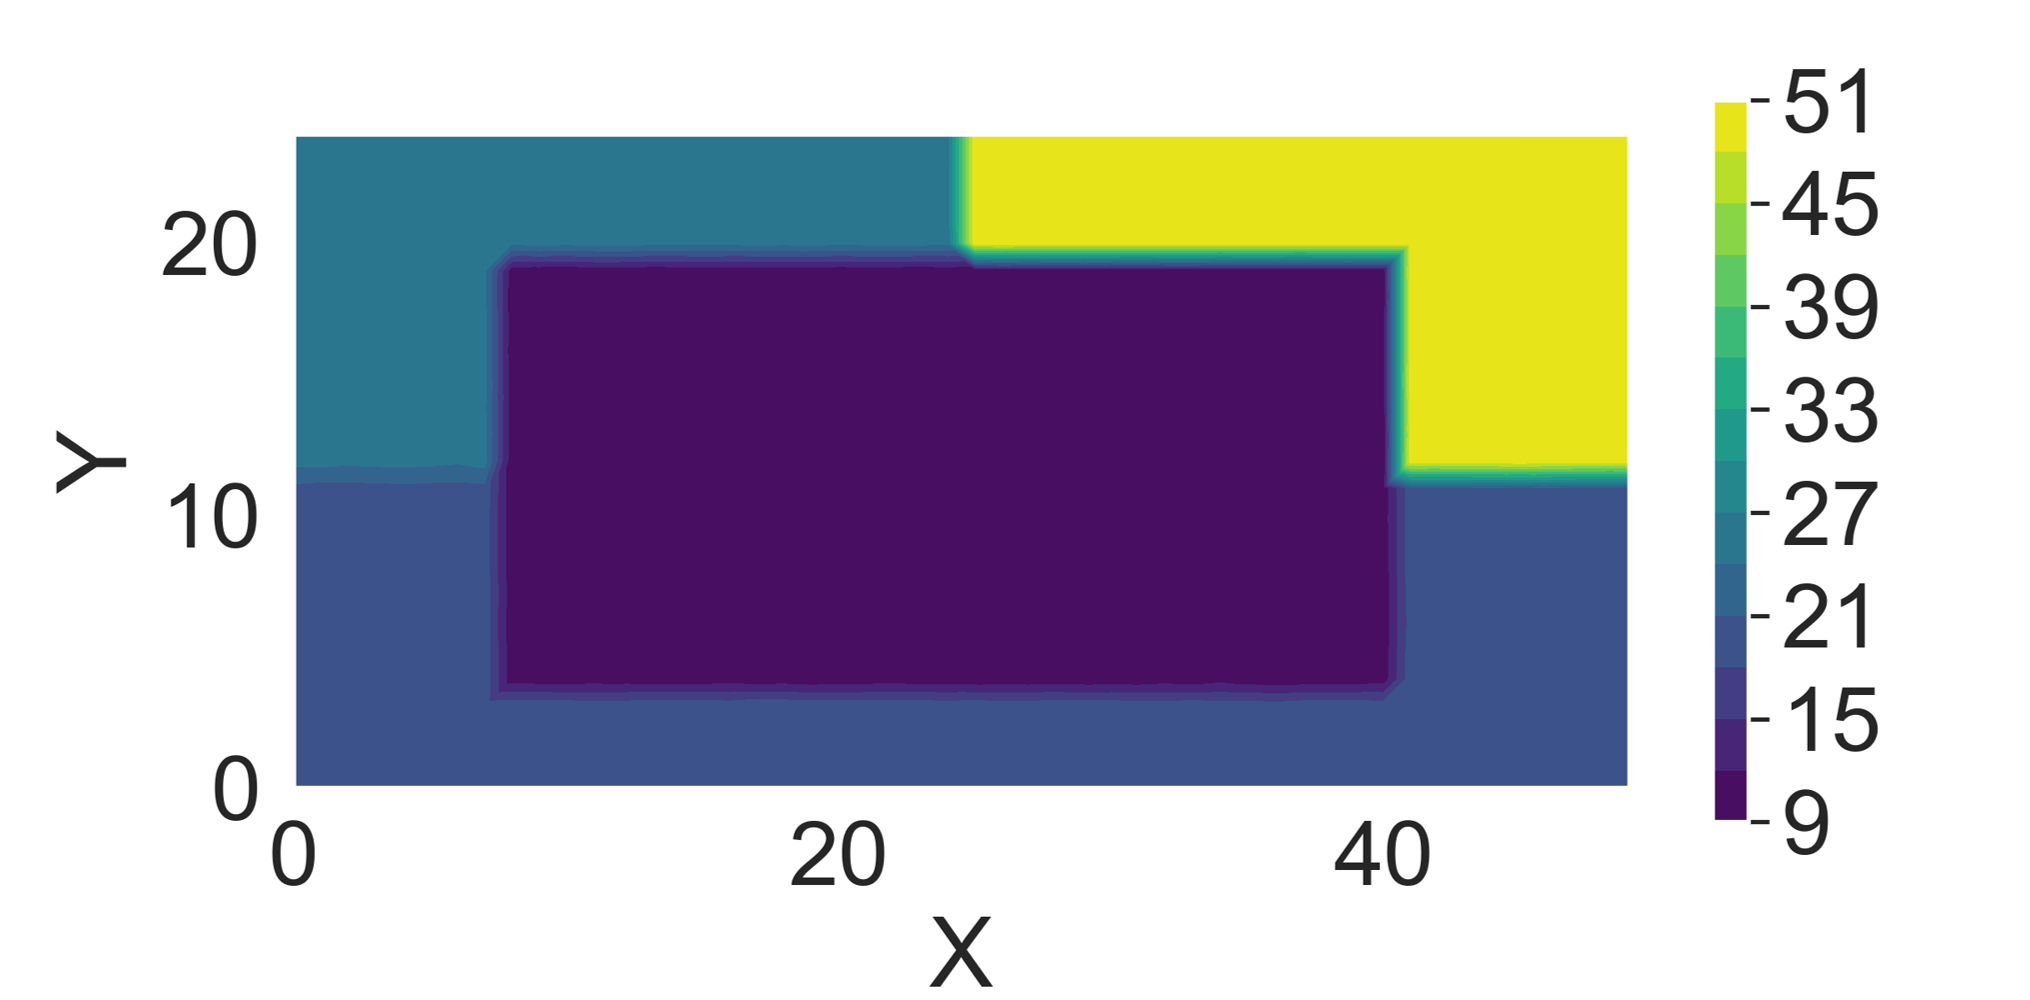
\includegraphics[width=0.9\linewidth]{pictures/E_map.png}
    }
\end{minipage}

\vspace{0.2em}

% --- Row 2 ---
\begin{minipage}{0.45\linewidth}
    \subfloat[$H/E$ ratio, dimensionless]{
        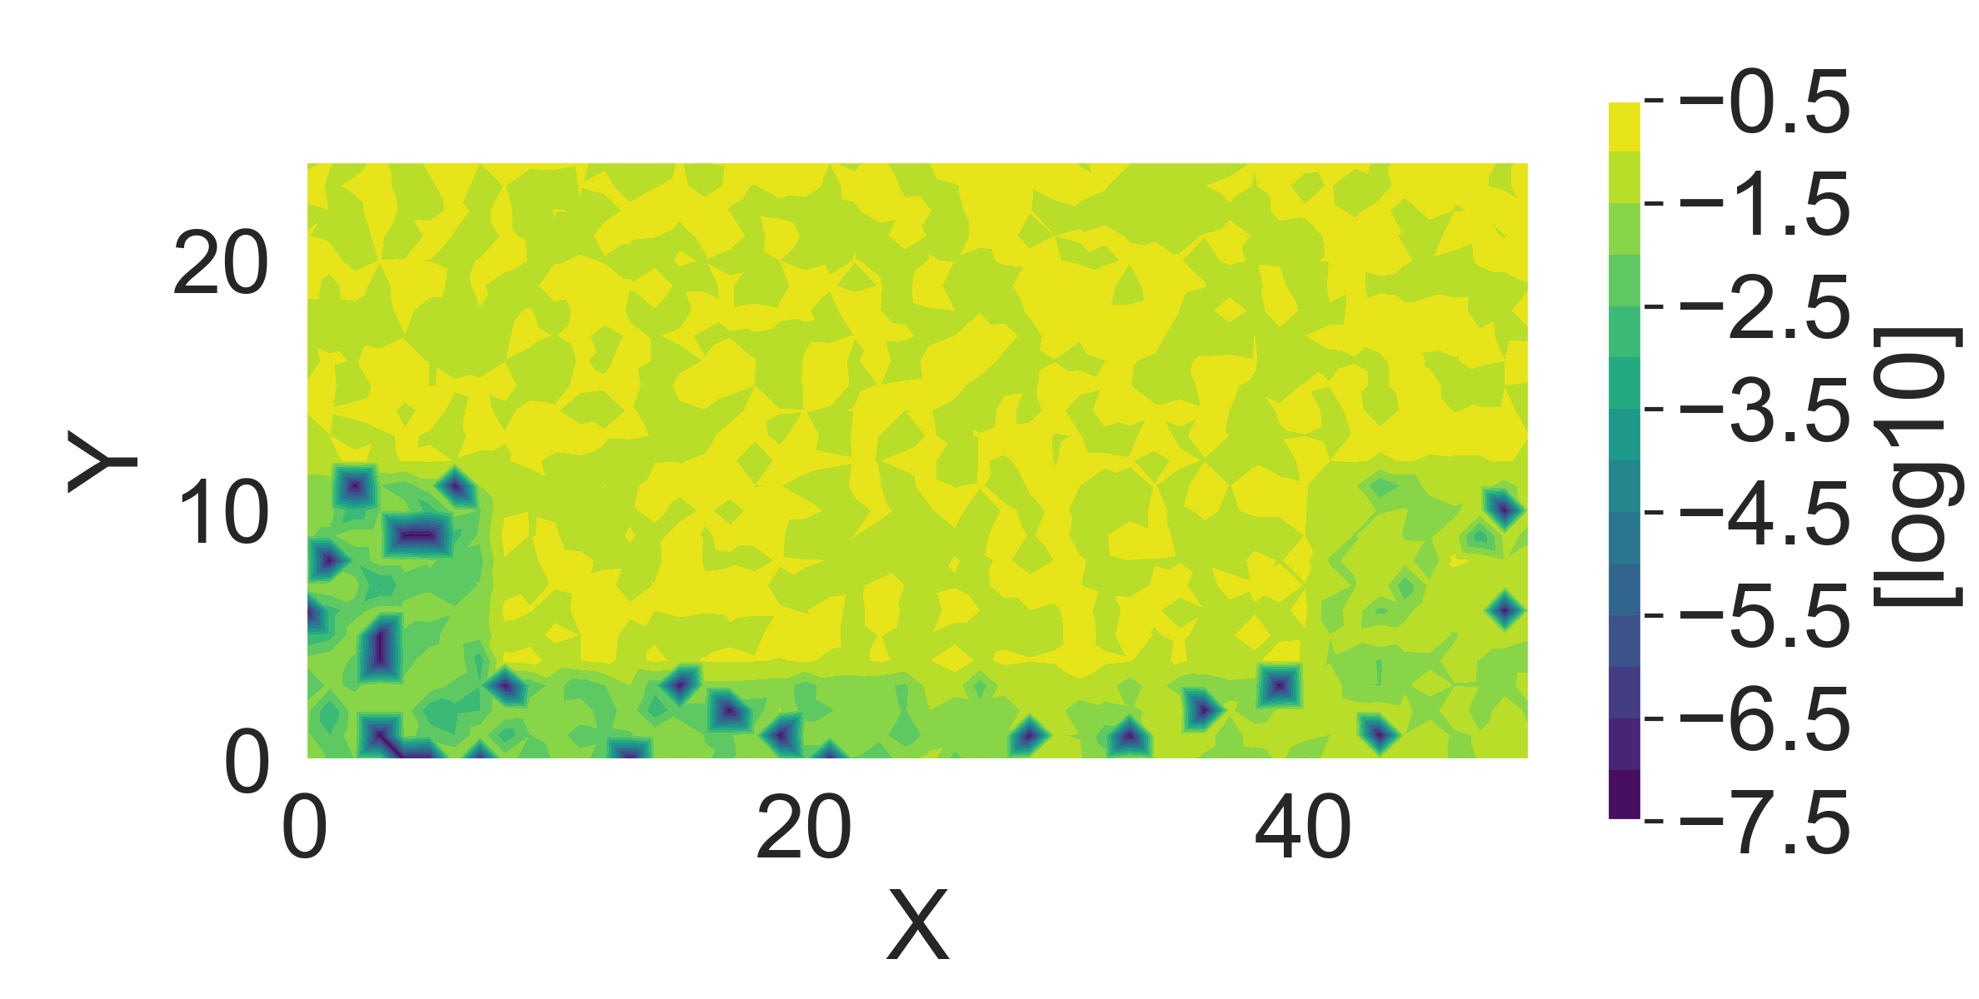
\includegraphics[width=0.9\linewidth]{pictures/HoverE.png}
    }
\end{minipage}
\hfill
\begin{minipage}{0.45\linewidth}
    \subfloat[$H^3/E^2$ ratio, units: GPa]{
        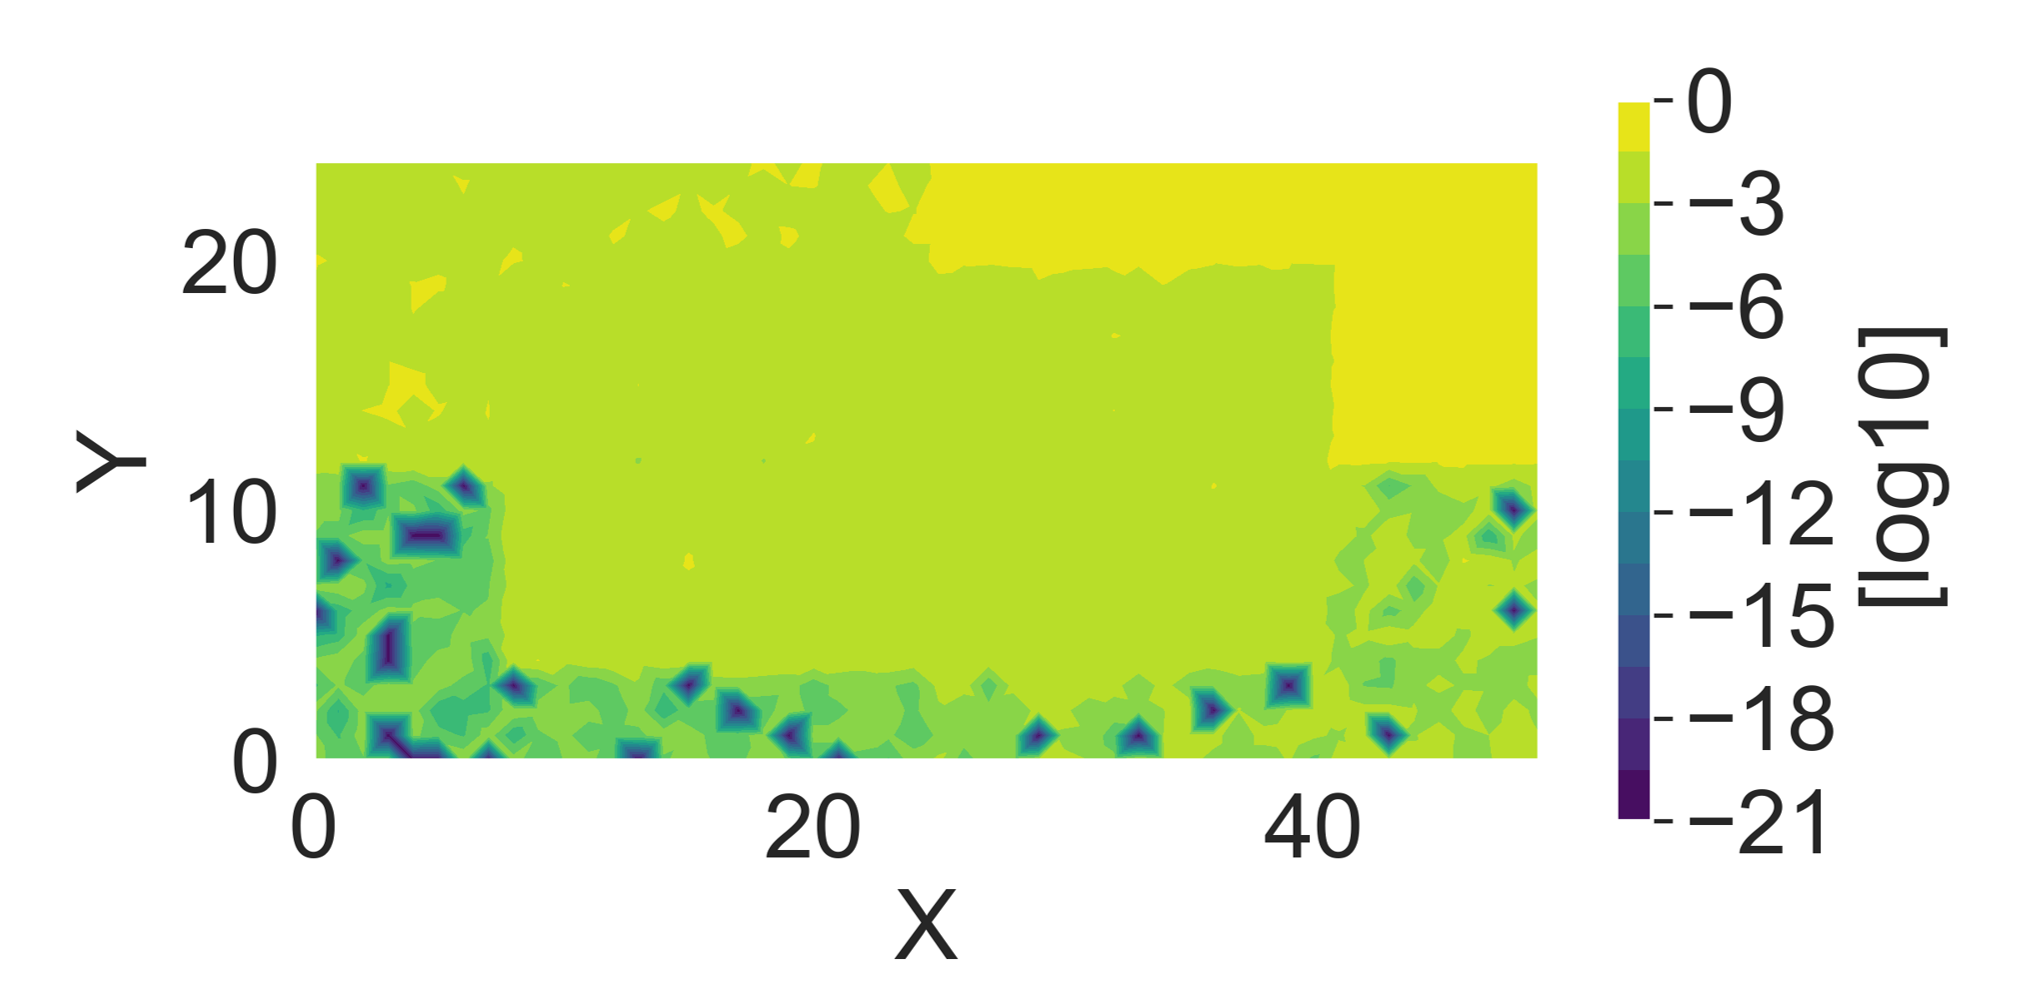
\includegraphics[width=0.9\linewidth]{pictures/H3overE2.png}
    }
\end{minipage}

\vspace{0.2em}

% --- Row 3 ---
\begin{minipage}{0.45\linewidth}
    \subfloat[KAMM (1st order), units: GPa$^2$]{
        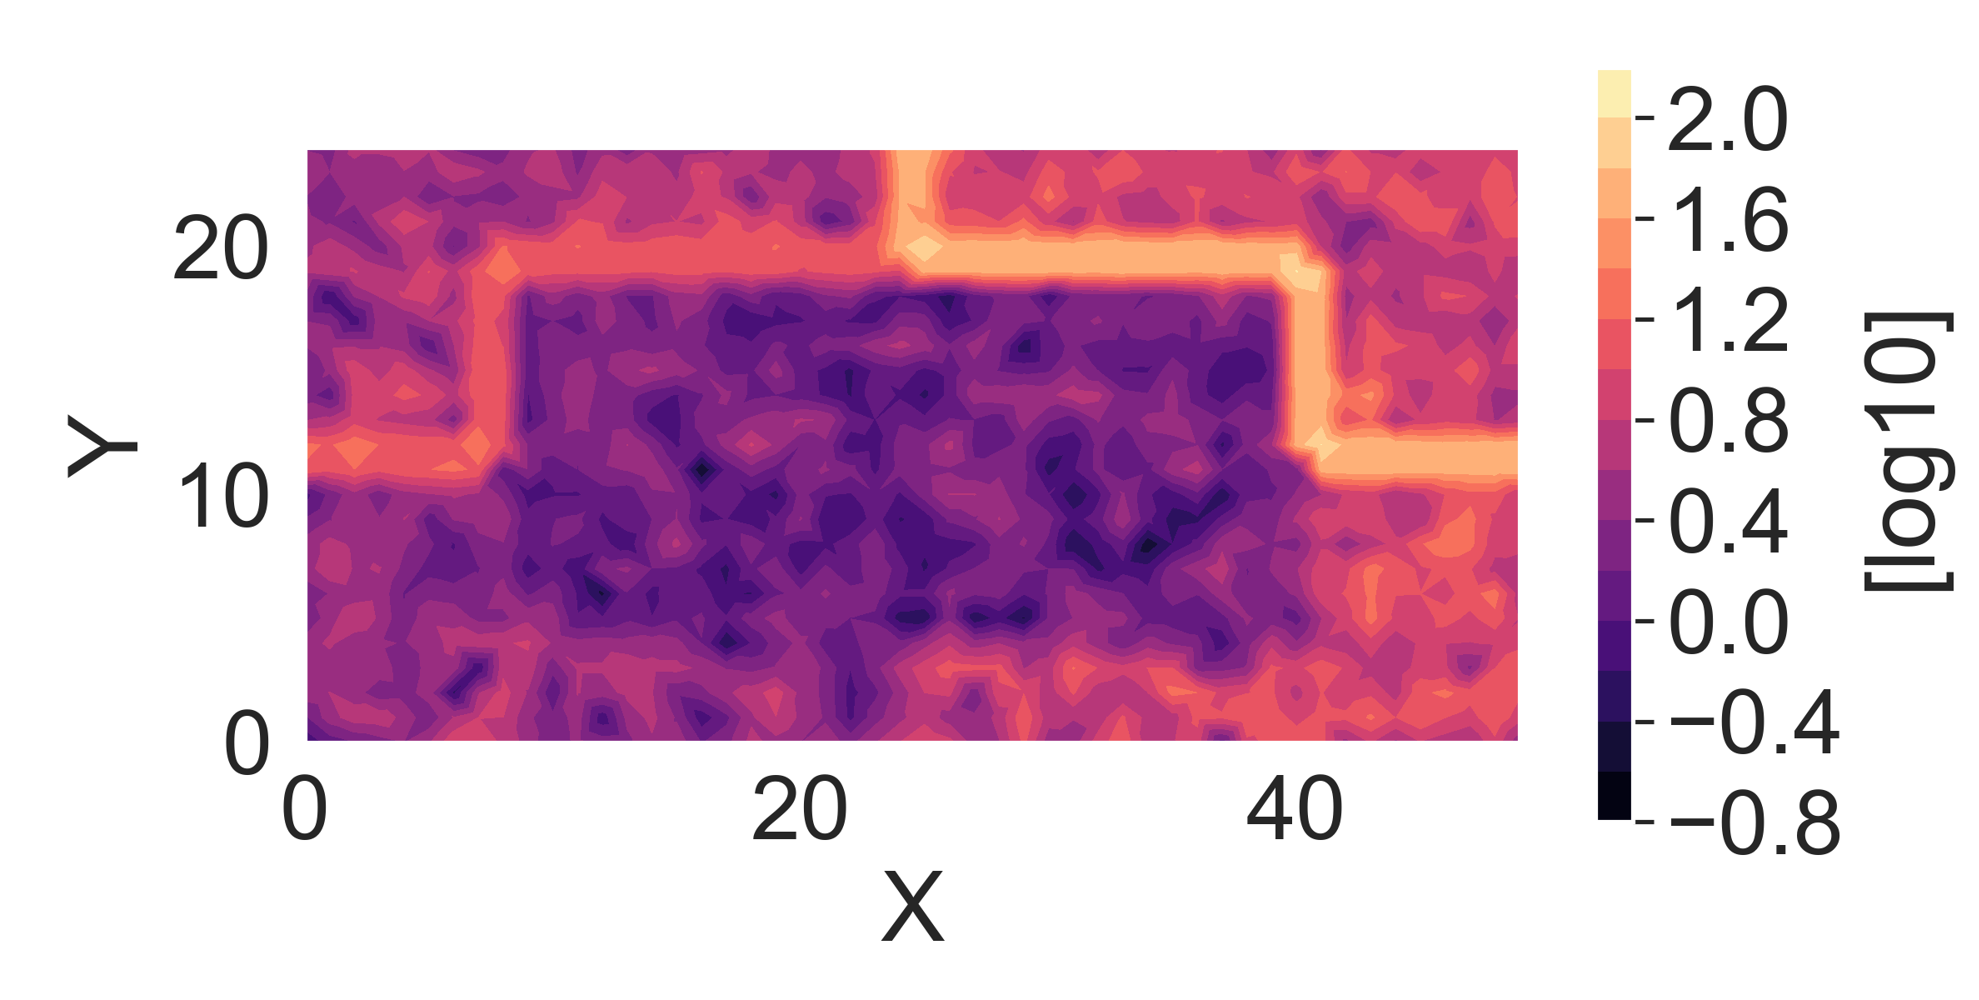
\includegraphics[width=0.9\linewidth]{pictures/KAMM.png}
    }
\end{minipage}
\hfill
\begin{minipage}{0.45\linewidth}
    \subfloat[KAMM (2nd order), units: GPa$^2$]{
        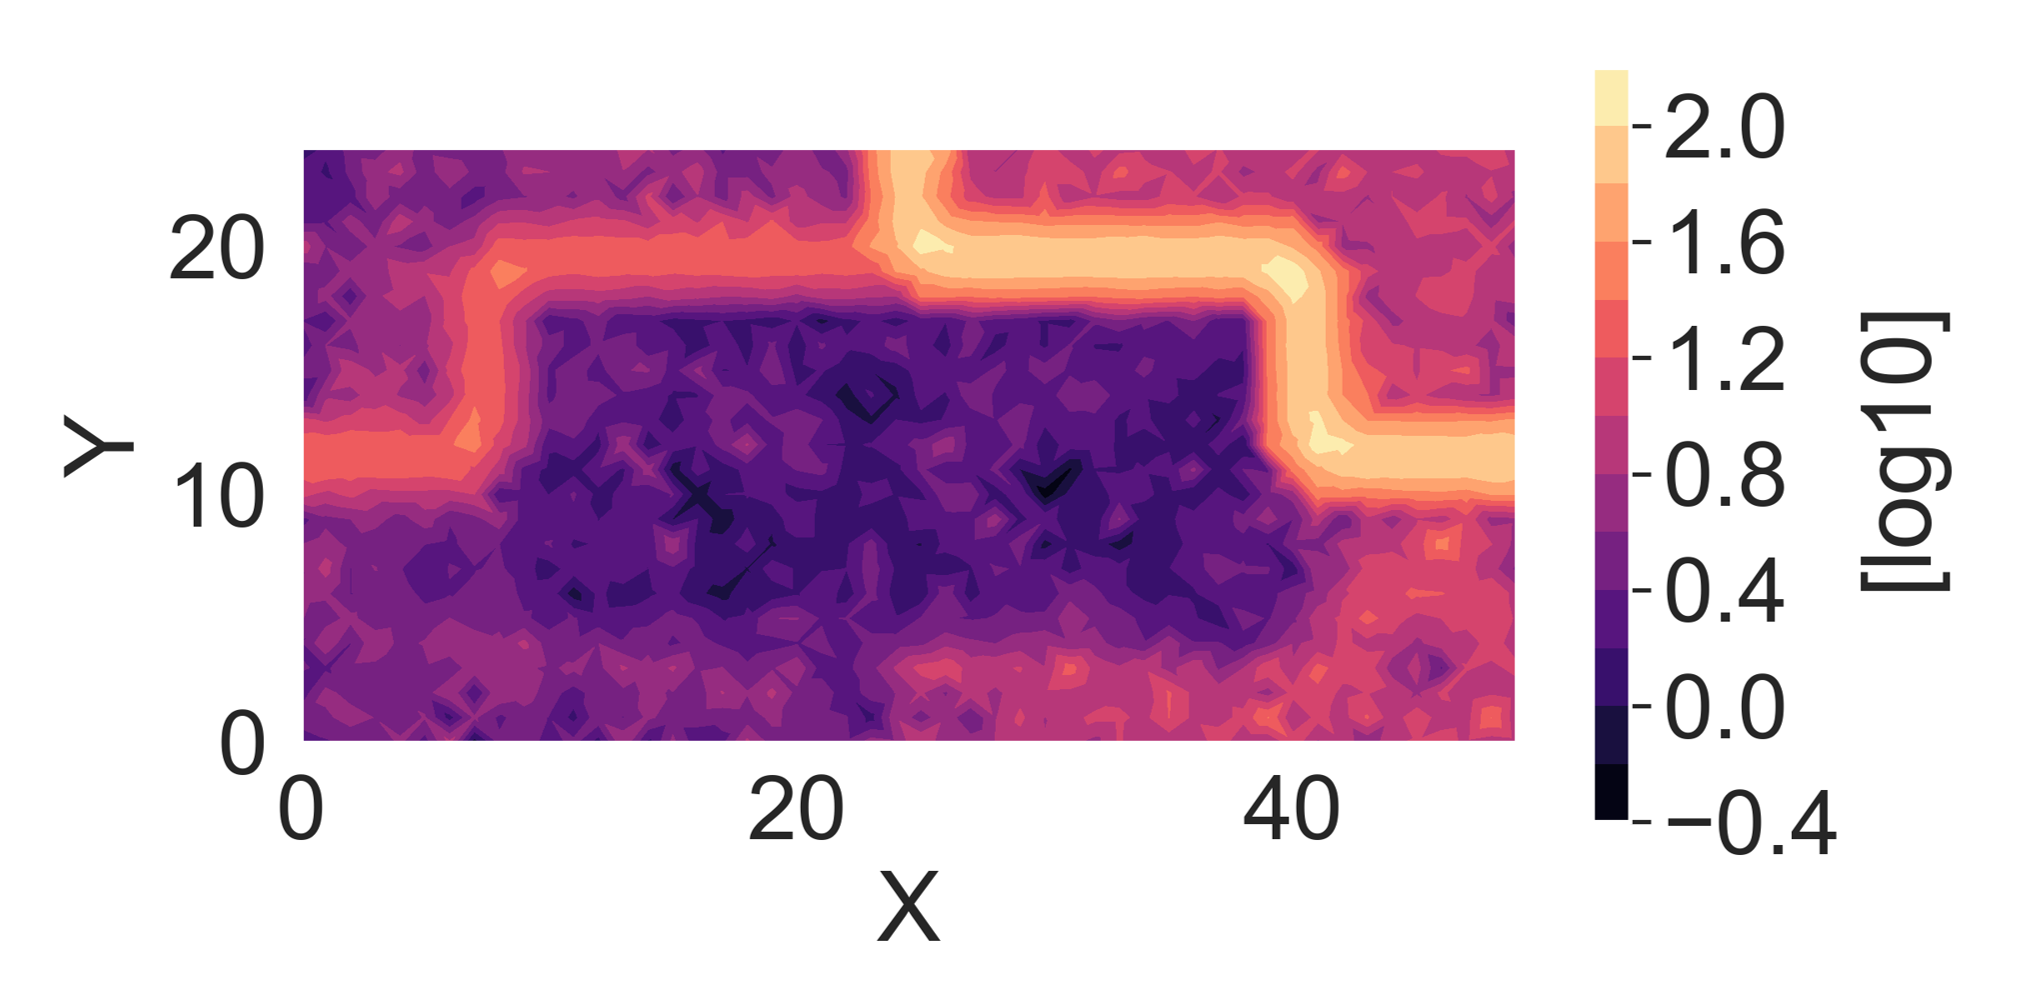
\includegraphics[width=0.9\linewidth]{pictures/KAMM_2.png}
    }
\end{minipage}

\vspace{0.2em}

% --- Row 4 ---
\begin{minipage}{0.45\linewidth}
    \subfloat[KAPM (hardness mismatch), units: GPa]{
        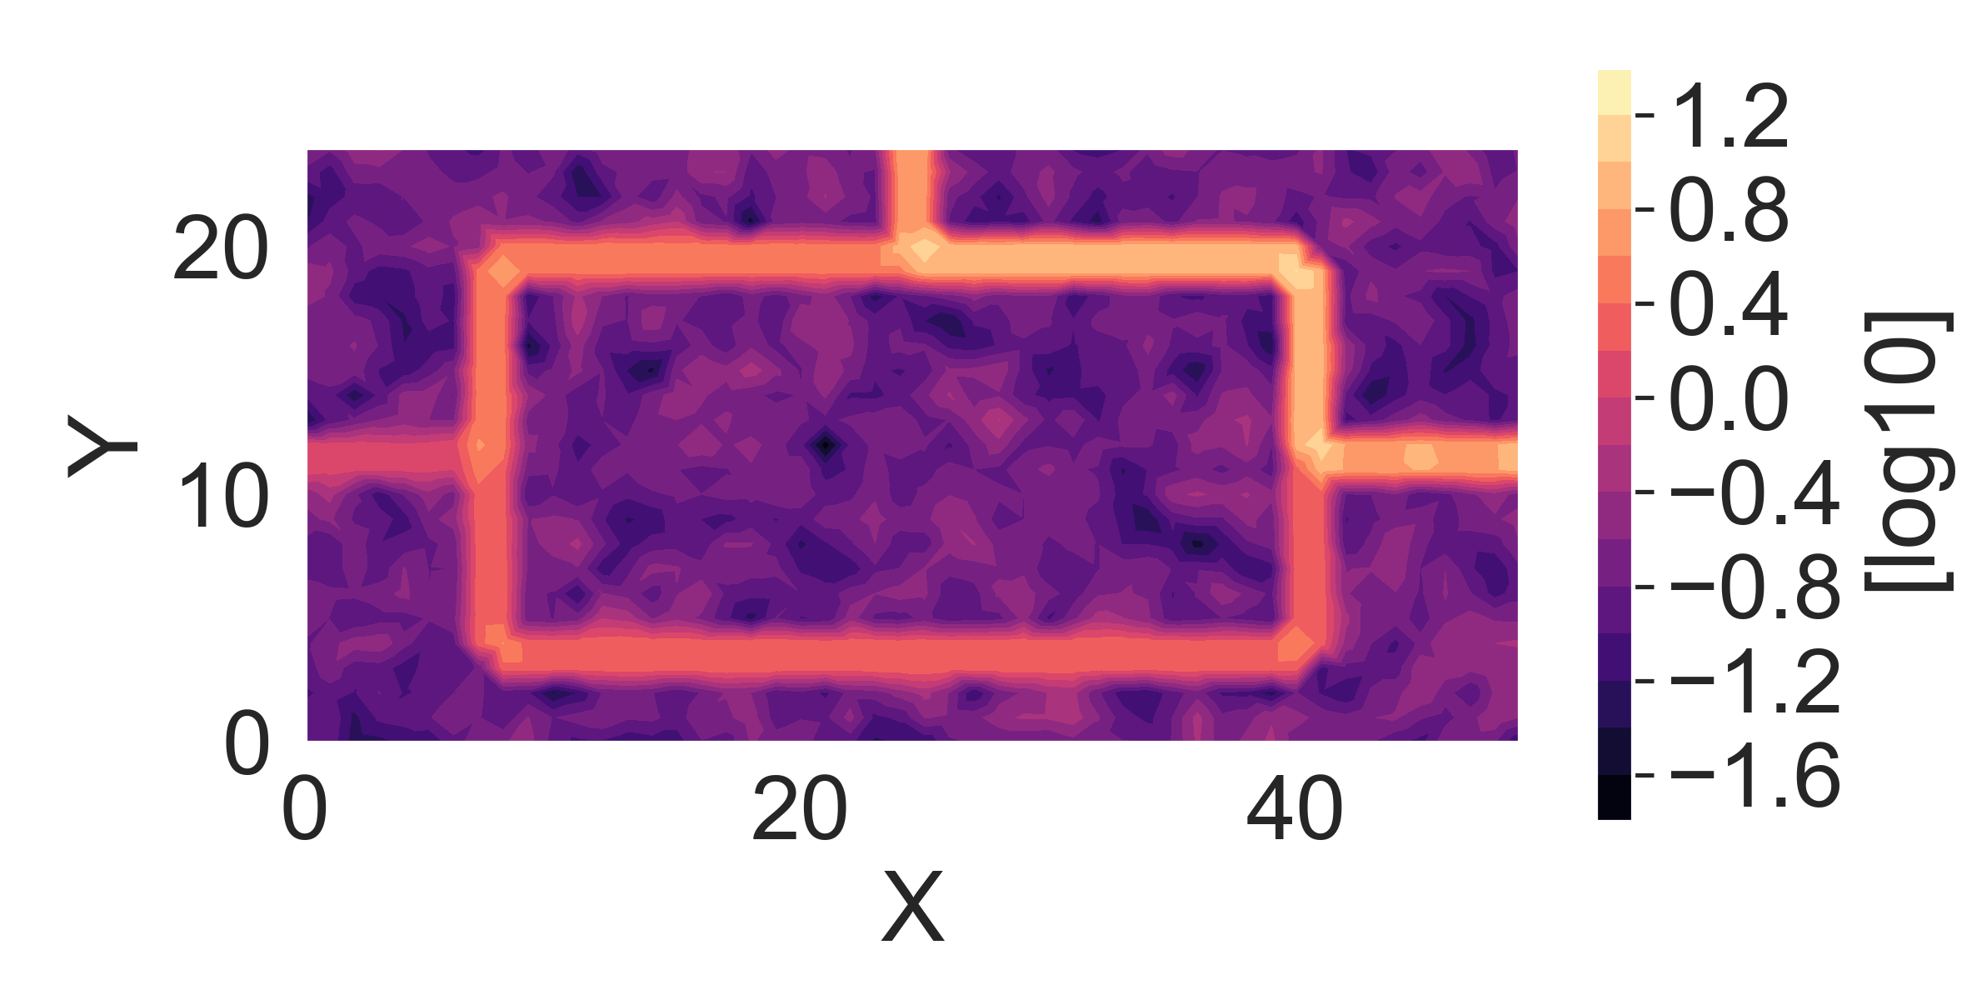
\includegraphics[width=0.9\linewidth]{pictures/KAPM.png}
    }
\end{minipage}
\hfill
\begin{minipage}{0.45\linewidth}
    \subfloat[KAEM (modulus mismatch), units: GPa]{
        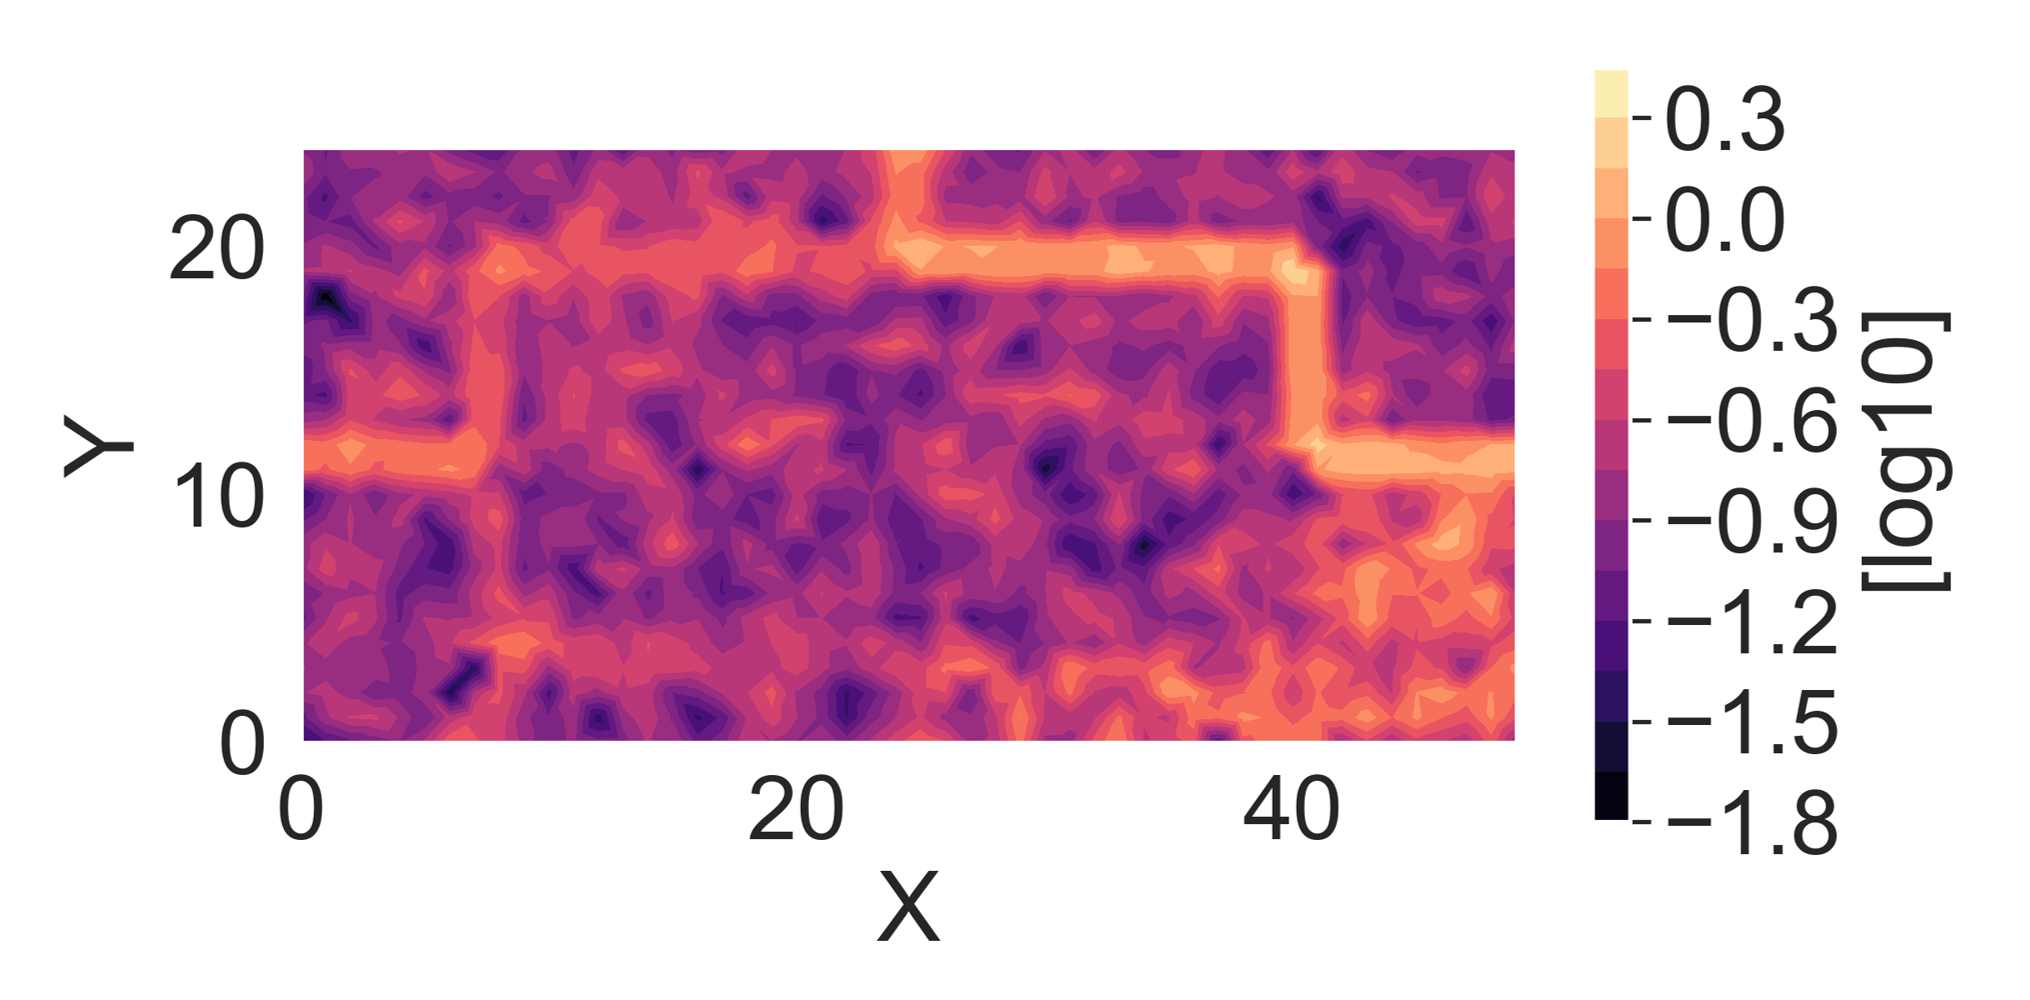
\includegraphics[width=0.9\linewidth]{pictures/KAEM.png}
    }
\end{minipage}

\vspace{0.2em}

% --- Row 5 ---
\begin{minipage}{0.49\linewidth}
    \subfloat[KAMM\textsubscript{RATIO}, dimensionless]{
        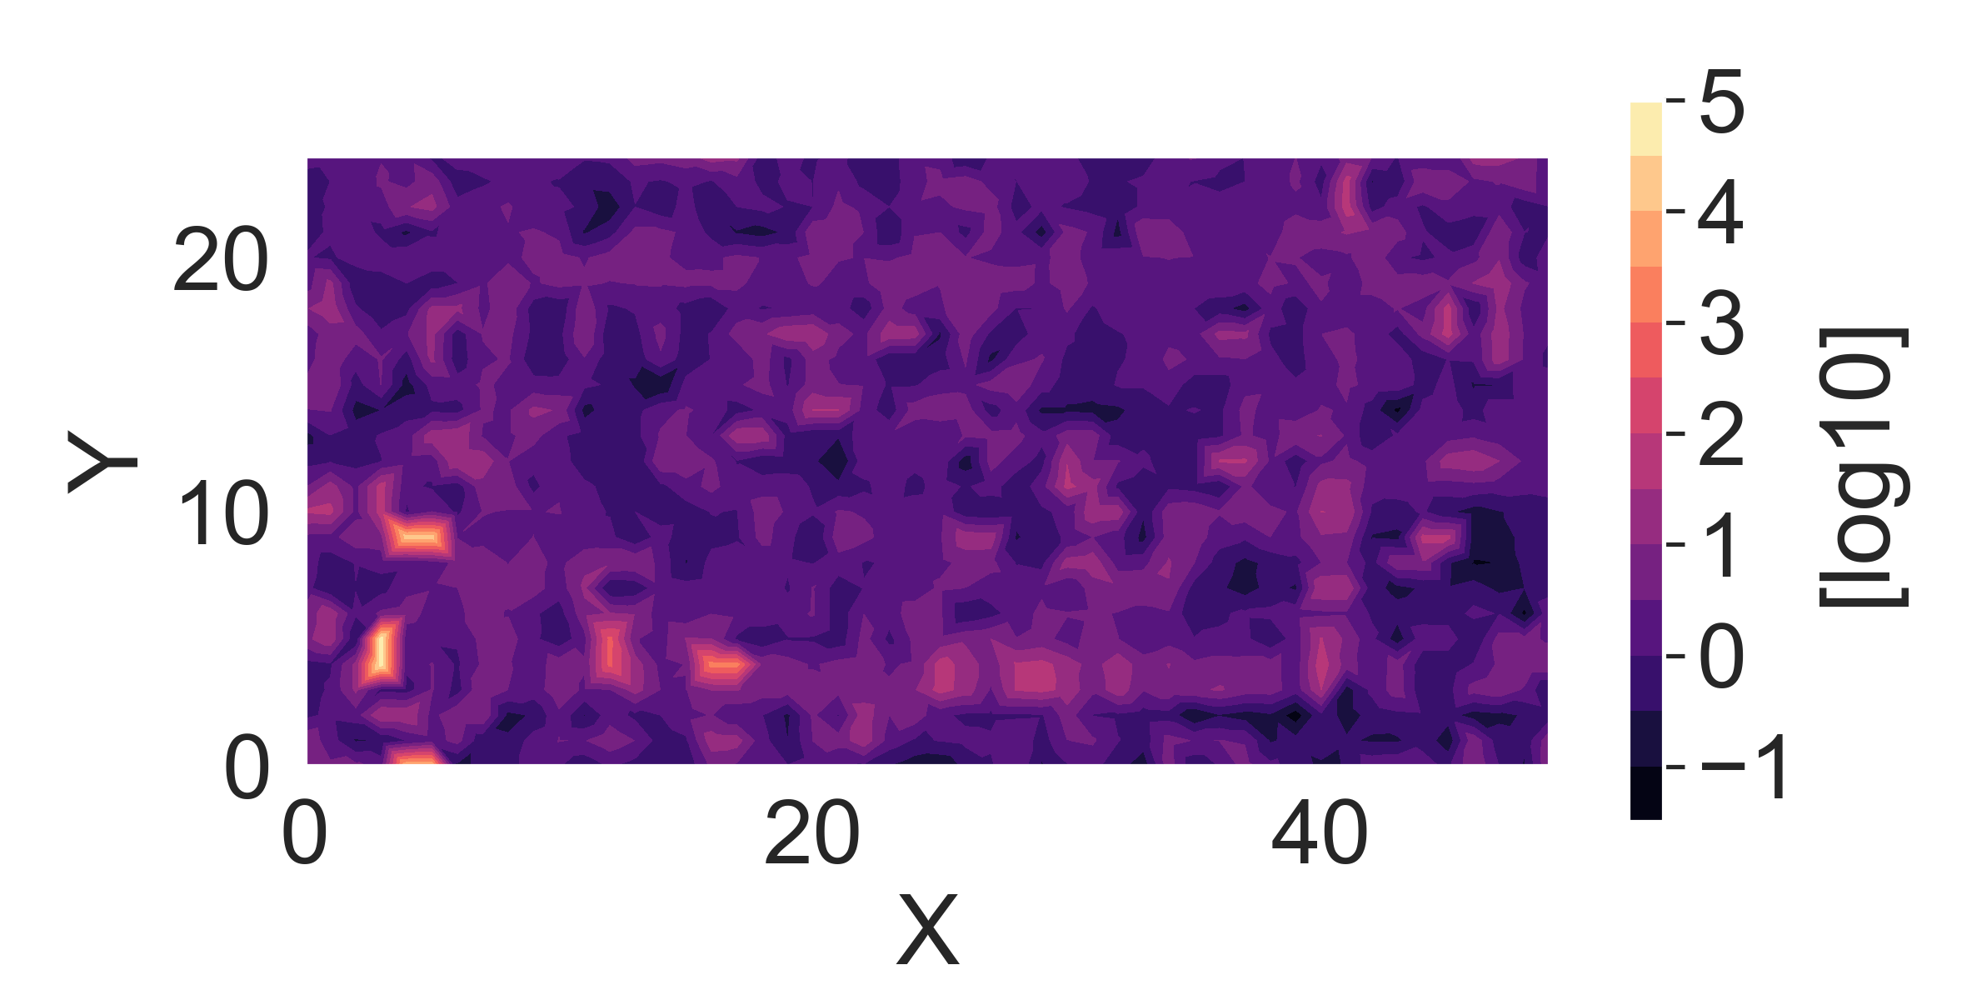
\includegraphics[width=0.9\linewidth]{pictures/KAMMratio.png}
    }
\end{minipage}
\hfill
\begin{minipage}{0.49\linewidth}
    \subfloat[KAMM\textsubscript{NORMPROD}, dimensionless]{
        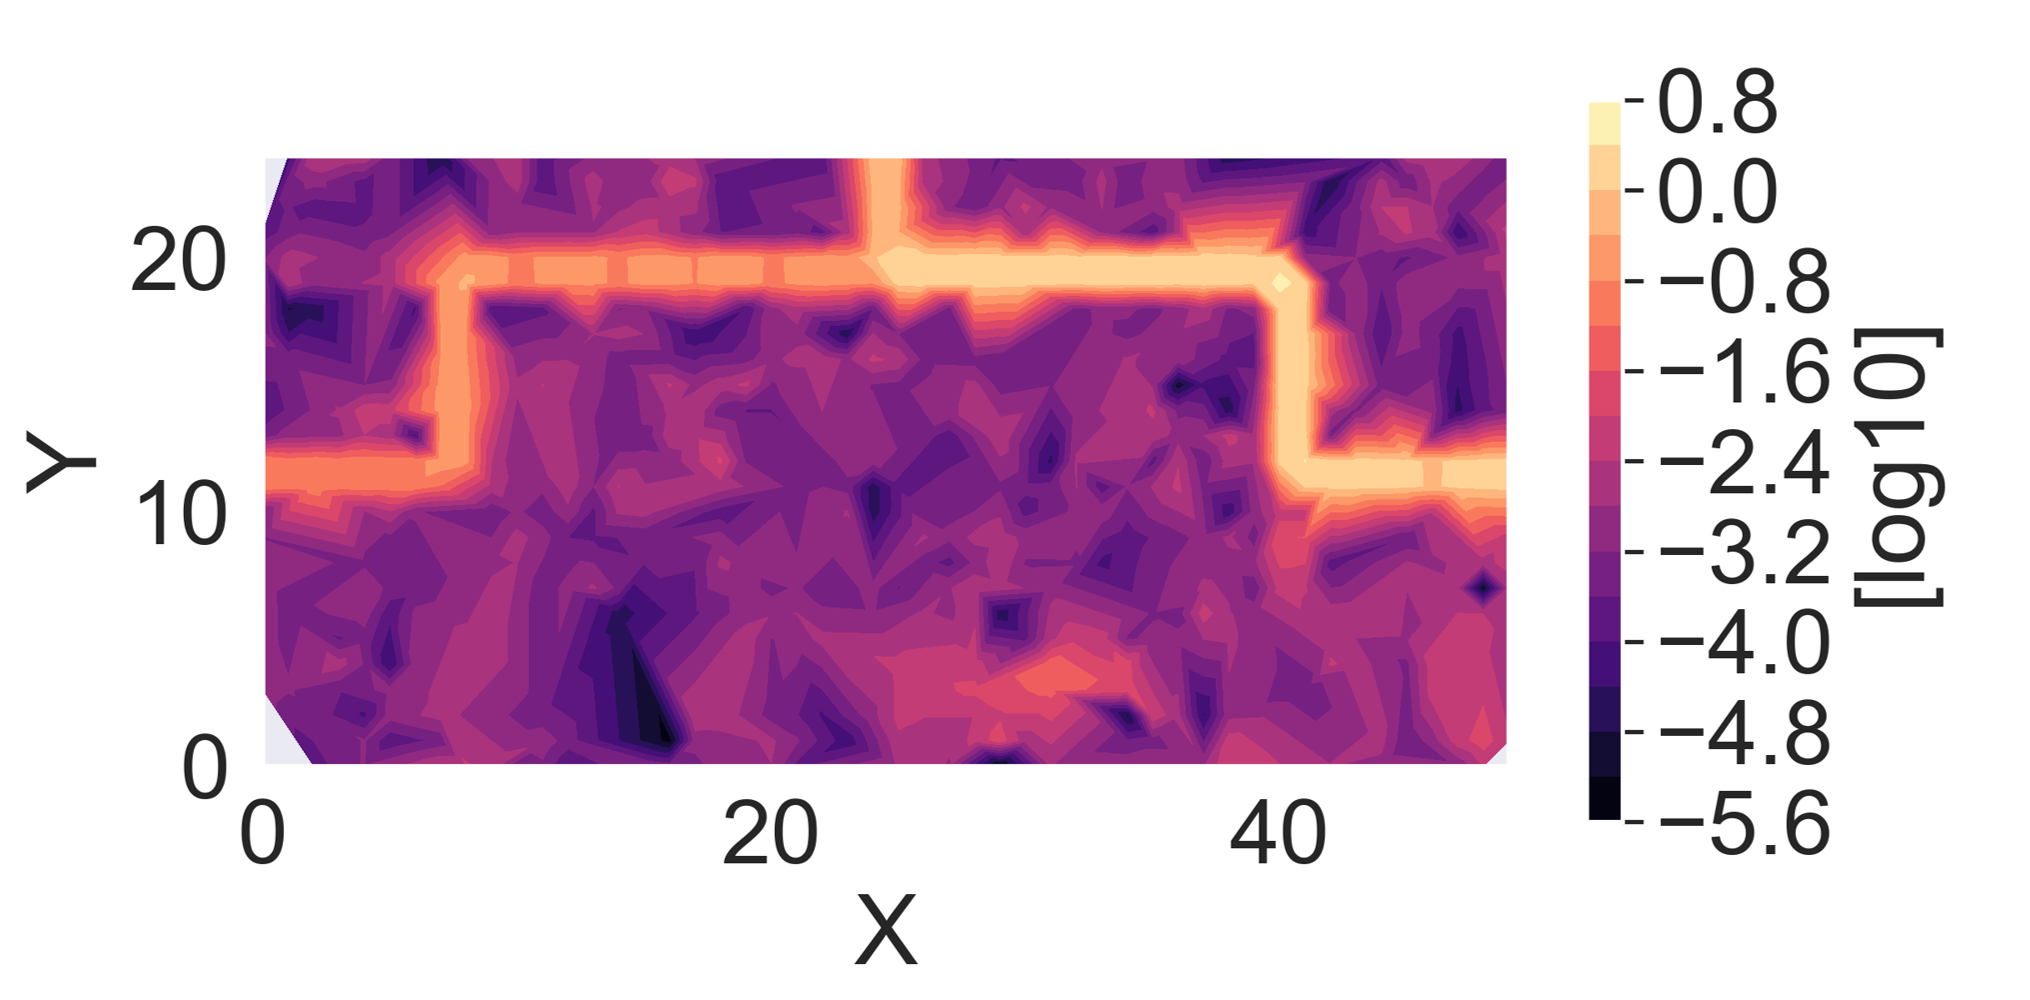
\includegraphics[width=0.9\linewidth]{pictures/KAMMprod.png}
    }
\end{minipage}

\caption{Local mechanical metrics computed on the five-region synthetic specimen: (a) hardness; (b) elastic modulus; (c) $H/E$ ratio; (d) $H^3/E^2$ ratio; (e) first-order KAMM; (f) second-order KAMM; (g) KAPM; (h) KAEM; (i) KAMM\textsubscript{RATIO}; and (j) KAMM\textsubscript{NORMPROD}. The neighborhood-based descriptors highlight different aspects of local mechanical heterogeneity and boundary contrast.}
\label{fig:five_regions_reference}
\end{figure}

The choice of neighborhood impacts sensitivity: $\mathcal{O}_1$ captures sharp phase boundaries, while $\mathcal{O}_2$ offers smoother transitions and broader gradient detection.

To illustrate the behavior of each feature, Figure~\ref{fig:five_regions_reference} shows the computed maps for hardness ($H$), modulus ($E$), scalar ratios ($H/E$, $H^3/E^2$), and the various KAM-based mismatch metrics using the five-region synthetic specimen. The ratio maps ($H/E$ and $H^3/E^2$) highlight differences in mechanical response across regions but often fail to capture precise boundaries or subtle interfacial transitions. In contrast, spatial mismatch metrics such as KAMM, KAEM, and KAPM produce stronger signals at phase boundaries and are particularly effective in highlighting interfaces when mechanical contrast is high. KAMM\textsubscript{RATIO} offers additional sensitivity within relatively homogeneous regions, revealing substructure or subtle measurement variability.

Notably, KAMM\textsubscript{NORMPROD} displays enhanced responses near triple junctions or corners, suggesting sensitivity to complex local variations that are less apparent in the base KAMM field. Blank pixels visible in some KAMM\textsubscript{RATIO} and KAMM\textsubscript{NORMPROD} maps correspond to non-finite descriptor values generated during feature calculation rather than to a physical absence of local variation. Their possible origins and their treatment by feature-wise mean imputation before standardization and clustering are described above.
\paragraph{Clustering pipeline and neighborhood-based integration}
To classify mechanically distinct regions in nanomechanical maps, we implemented a modular and reproducible clustering pipeline. After importing raw indentation data (CSV or Excel), the pipeline performs initial preprocessing, including header normalization, numerical cleaning, and optional computation of dimensionless mechanical ratios such as $H/E$ and $H^3/E^2$.

When neighborhood-based awareness is required, the pipeline computes kernel-based descriptors-specifically KAMM, KAEM, KAPM, KAMM\textsubscript{RATIO}, and KAMM\textsubscript{NORMPROD}-using either first- or second-order neighborhoods. These spatial features capture local mechanical mismatches and gradients, enriching the dataset beyond global $(E, H)$ values. By appending KAMM-based features to the $(E, H)$ feature space, the clustering process becomes both mechanically and neighborhood-informed. This provides additional information on interphase regions and ambiguous transition zones that may otherwise be difficult to distinguish using $(E,H)$ alone. As shown in Section~\ref{sec:results}, the influence of KAMM depends on the clustering algorithm, microstructural configuration, and noise level, with improvements observed for selected combinations and limited or negative effects for others.

Following feature construction, all selected variables are standardized using z-score normalization implemented via the \textit{scikit-learn} library~\cite{scikit-learn, sklearn_api}. Dimensionality reduction and visualization are optionally performed using Principal Component Analysis (PCA), also from \textit{scikit-learn}. Clustering is carried out with four unsupervised algorithms provided by the same library: agglomerative clustering (hierarchical), DBSCAN (density-based), Gaussian Mixture Models (probabilistic), and KMeans (distance-based). The algorithms are applied in a consistent order to facilitate comparison across figures and datasets.

The number of clusters can be defined manually or estimated automatically (e.g., using the elbow method based on the KMeans inertia). In this study, the number of clusters is fixed to 2 for specimens a, d, and f (no interphase), and to 3 for all specimens containing interphases, ensuring a consistent comparison across the four algorithms. For DBSCAN, although the algorithm does not inherently require a predefined number of clusters, its hyperparameters ($\varepsilon$ and \textit{min\_samples}) are systematically tuned such that the number of detected non-noise clusters matches the prescribed target ($k = 2$ or $k = 3$), thereby enforcing methodological consistency across all clustering approaches. This tuning strategy was adopted solely to enable direct comparison with clustering methods requiring a prescribed number of clusters. We acknowledge that this approach does not fully exploit the intrinsic strengths of DBSCAN and therefore represents a limitation of the present benchmarking strategy.

\paragraph{Clustering evaluation and error analysis} Cluster assignments are first mapped back to the spatial domain and projected into feature space to facilitate interpretation. Each cluster is associated with a reference phase according to ascending mean hardness, ensuring a physically consistent ordering under the assumption of monotonic mechanical contrast. For each identified phase, statistical summaries (such as volume fraction and the mean and standard deviation of $E$ and $H$) are computed and exported together with the corresponding visualizations. For synthetic datasets, where ground-truth phase labels are available, clustering performance is primarily evaluated using pixel-level accuracy, defined as the fraction of grid points for which the predicted cluster label matches the ground-truth phase label. This metric is evaluated over a range of mechanical contrast ratios $(H_\mathrm{ratio}, E_\mathrm{ratio})$, clustering algorithms, and configurations with or without KAMM-based spatial features. When analyzing accuracy as a function of hardness contrast, the reported curves correspond to an average over all sampled elastic modulus contrast ratios. Specifically, for each value of $H_\mathrm{ratio}$, pixel-level accuracy is computed as the mean accuracy across the full set of $E_\mathrm{ratio}$ values. This aggregation isolates the influence of hardness contrast while marginalizing variations in elastic stiffness contrast. Phase-specific mechanical properties are not introduced as a separate supervised performance metric in the synthetic benchmark. Instead, the mean and standard deviation of $E$ and $H$ within the identified clusters are used as complementary descriptive quantities, particularly when interpreting the experimental dataset. In a second step, intrinsic clustering quality is assessed using unsupervised metrics, including the Silhouette score, Calinski--Harabasz index, and Davies--Bouldin index. These scores quantify cluster compactness and separation independently of ground truth, enabling systematic comparison across datasets and clustering strategies~\cite{Rubinos_2024}.

\subsection{Descriptor sensitivity and feature variants}

Several neighborhood descriptors were investigated, including KAEM, KAPM, KAMM, KAMM\_RATIO and KAMM\_NORMPROD, together with first- and second-order neighborhoods. The objective was not to identify a single universally optimal descriptor, but to evaluate how different mismatch definitions influence boundary sensitivity, spatial coherence and phase recovery. The five-region benchmark presented in Fig.~\ref{fig:five_regions_reference} provides a qualitative comparison of these descriptors. While all variants highlight mechanical heterogeneity, the resulting spatial patterns differ significantly. KAEM and KAPM emphasize modulus and hardness contrasts separately, whereas KAMM combines both responses in a single indicator. Higher-order descriptors increase sensitivity to local gradients and heterogeneous regions but may also amplify noise and feature-space redundancy.

% ----------------------------------------------------------
% 3. Results and Discussion
% ----------------------------------------------------------
\section{Results and Discussion}
\label{sec:results}

To evaluate the impact of KAMM features, we assessed the clustering accuracy of four standard algorithms (Agglomerative Clustering, DBSCAN, GMM, and KMeans) using synthetic composite specimens with progressively increasing interphase widths ($W = 0$, $0.03$, $0.05$). The input features were standardized using z-score scaling prior to clustering, and no dimensionality reduction (e.g., PCA) was applied. Accuracy is reported as a function of the hardness contrast $H_\mathrm{ratio}$, with solid curves representing KAMM (1st-order)-enhanced clustering and dashed curves indicating the baseline $(E,H)$-only approach. Different colors denote the various interphase widths, enabling direct comparison of algorithm performance under increasing boundary complexity. The same general comparison between baseline and KAMM-augmented feature spaces is used throughout the synthetic Results sections, with the specific geometry, interphase width, and noise conditions stated in each subsection.

\subsection{Rectangular composite: effect of interphase width on clustering accuracy} \label{sec:results_interphasewidth}

Figure~\ref{fig:accuracy_matrix} presents the full three-dimensional (3D) accuracy landscapes, where pixel-level clustering accuracy is mapped as a function of both hardness contrast ($H_\mathrm{ratio}$) and elastic modulus contrast ($E_\mathrm{ratio}$). These maps provide the complete contrast-dependent behavior for each algorithm. From these surfaces, two-dimensional (2D) accuracy profiles are obtained by averaging over all sampled $E_\mathrm{ratio}$ values. The resulting curves, shown in Fig.~\ref{fig:kamm_accuracy_comparison}, therefore represent hardness-dependent projections of the full 3D accuracy maps and summarize the global trend with respect to mechanical contrast. Overall, these results indicate that incorporating KAMM-based spatial descriptors generally improves clustering performance for most algorithms, particularly centroid- and distribution-based methods such as KMeans and GMM.

Quantitatively, the mean pixel-level accuracy of KMeans increases from 0.689 to 0.823 with KAMM, while GMM improves from 0.737 to 0.833. This behavior is consistent with the underlying assumptions of these methods: both rely on global structure in feature space (cluster centroids or Gaussian components), and the addition of spatial descriptors enhances inter-phase separability and cluster coherence. In contrast, DBSCAN exhibits reduced performance when KAMM features are included. As a density-based method, its clustering behavior is sensitive to changes in feature-space geometry, and the inclusion of neighborhood-derived descriptors can weaken density contrasts between phases. Accordingly, DBSCAN generally performs better without KAMM, particularly at higher $H$ ratios and larger interphase widths. Agglomerative clustering shows moderate improvement with KAMM, suggesting that hierarchical linkage criteria benefit from enhanced spatial coherence while remaining less sensitive to density distortions than DBSCAN.

From the intrinsic clustering metrics averaged over all contrast ratios, KMeans without KAMM provides the highest Silhouette score (0.047) and Calinski-Harabasz index (529.8), while Agglomerative clustering yields the lowest Davies-Bouldin index (1.85), indicating the most compact and well-separated clusters in feature space. When KAMM is included, these internal metrics decrease for all centroid- and linkage-based methods: for KMeans, the Silhouette score drops from 0.047 to -0.013, the Calinski-Harabasz index decreases from 529.8 to 34.7, and the Davies-Bouldin index increases from 5.58 to 24.48. GMM shows a similar reduction in Calinski-Harabasz (371.3 to 85.1) and increase in Davies-Bouldin (5.04 to 26.36). DBSCAN exhibits consistently negative Silhouette values (-0.339 without KAMM and -0.503 with KAMM), reflecting limited cluster compactness under density-based assumptions. Overall, although KAMM improves pixel-level classification accuracy for several algorithm--configuration combinations, it reduces standard unsupervised compactness and separation indices across methods. This apparent contradiction arises because the two categories of metrics evaluate fundamentally different objectives. Pixel-level accuracy measures agreement with the known phase labels available in the synthetic benchmarks and therefore directly assesses phase recovery. In contrast, the Silhouette score, Calinski--Harabasz index, and Davies--Bouldin index quantify compactness and separation in feature space without reference to the underlying microstructure. KAMM intentionally introduces neighborhood information that emphasizes interfaces, interphases, and mechanically heterogeneous transition regions, which do not necessarily form compact or well-separated clusters in feature space. Consequently, improved agreement with the known phase labels may occur even when conventional unsupervised clustering metrics decrease. For the synthetic benchmarks considered here, pixel-level accuracy is therefore used as the primary supervised measure of phase recovery, while the unsupervised metrics provide complementary information on feature-space compactness and separation.

Finally, no systematic influence of interphase width on clustering accuracy is observed within the investigated range, indicating that diffuse interfaces do not significantly compromise phase separability in the adopted feature representations.

\begin{figure}[htbp]
\centering
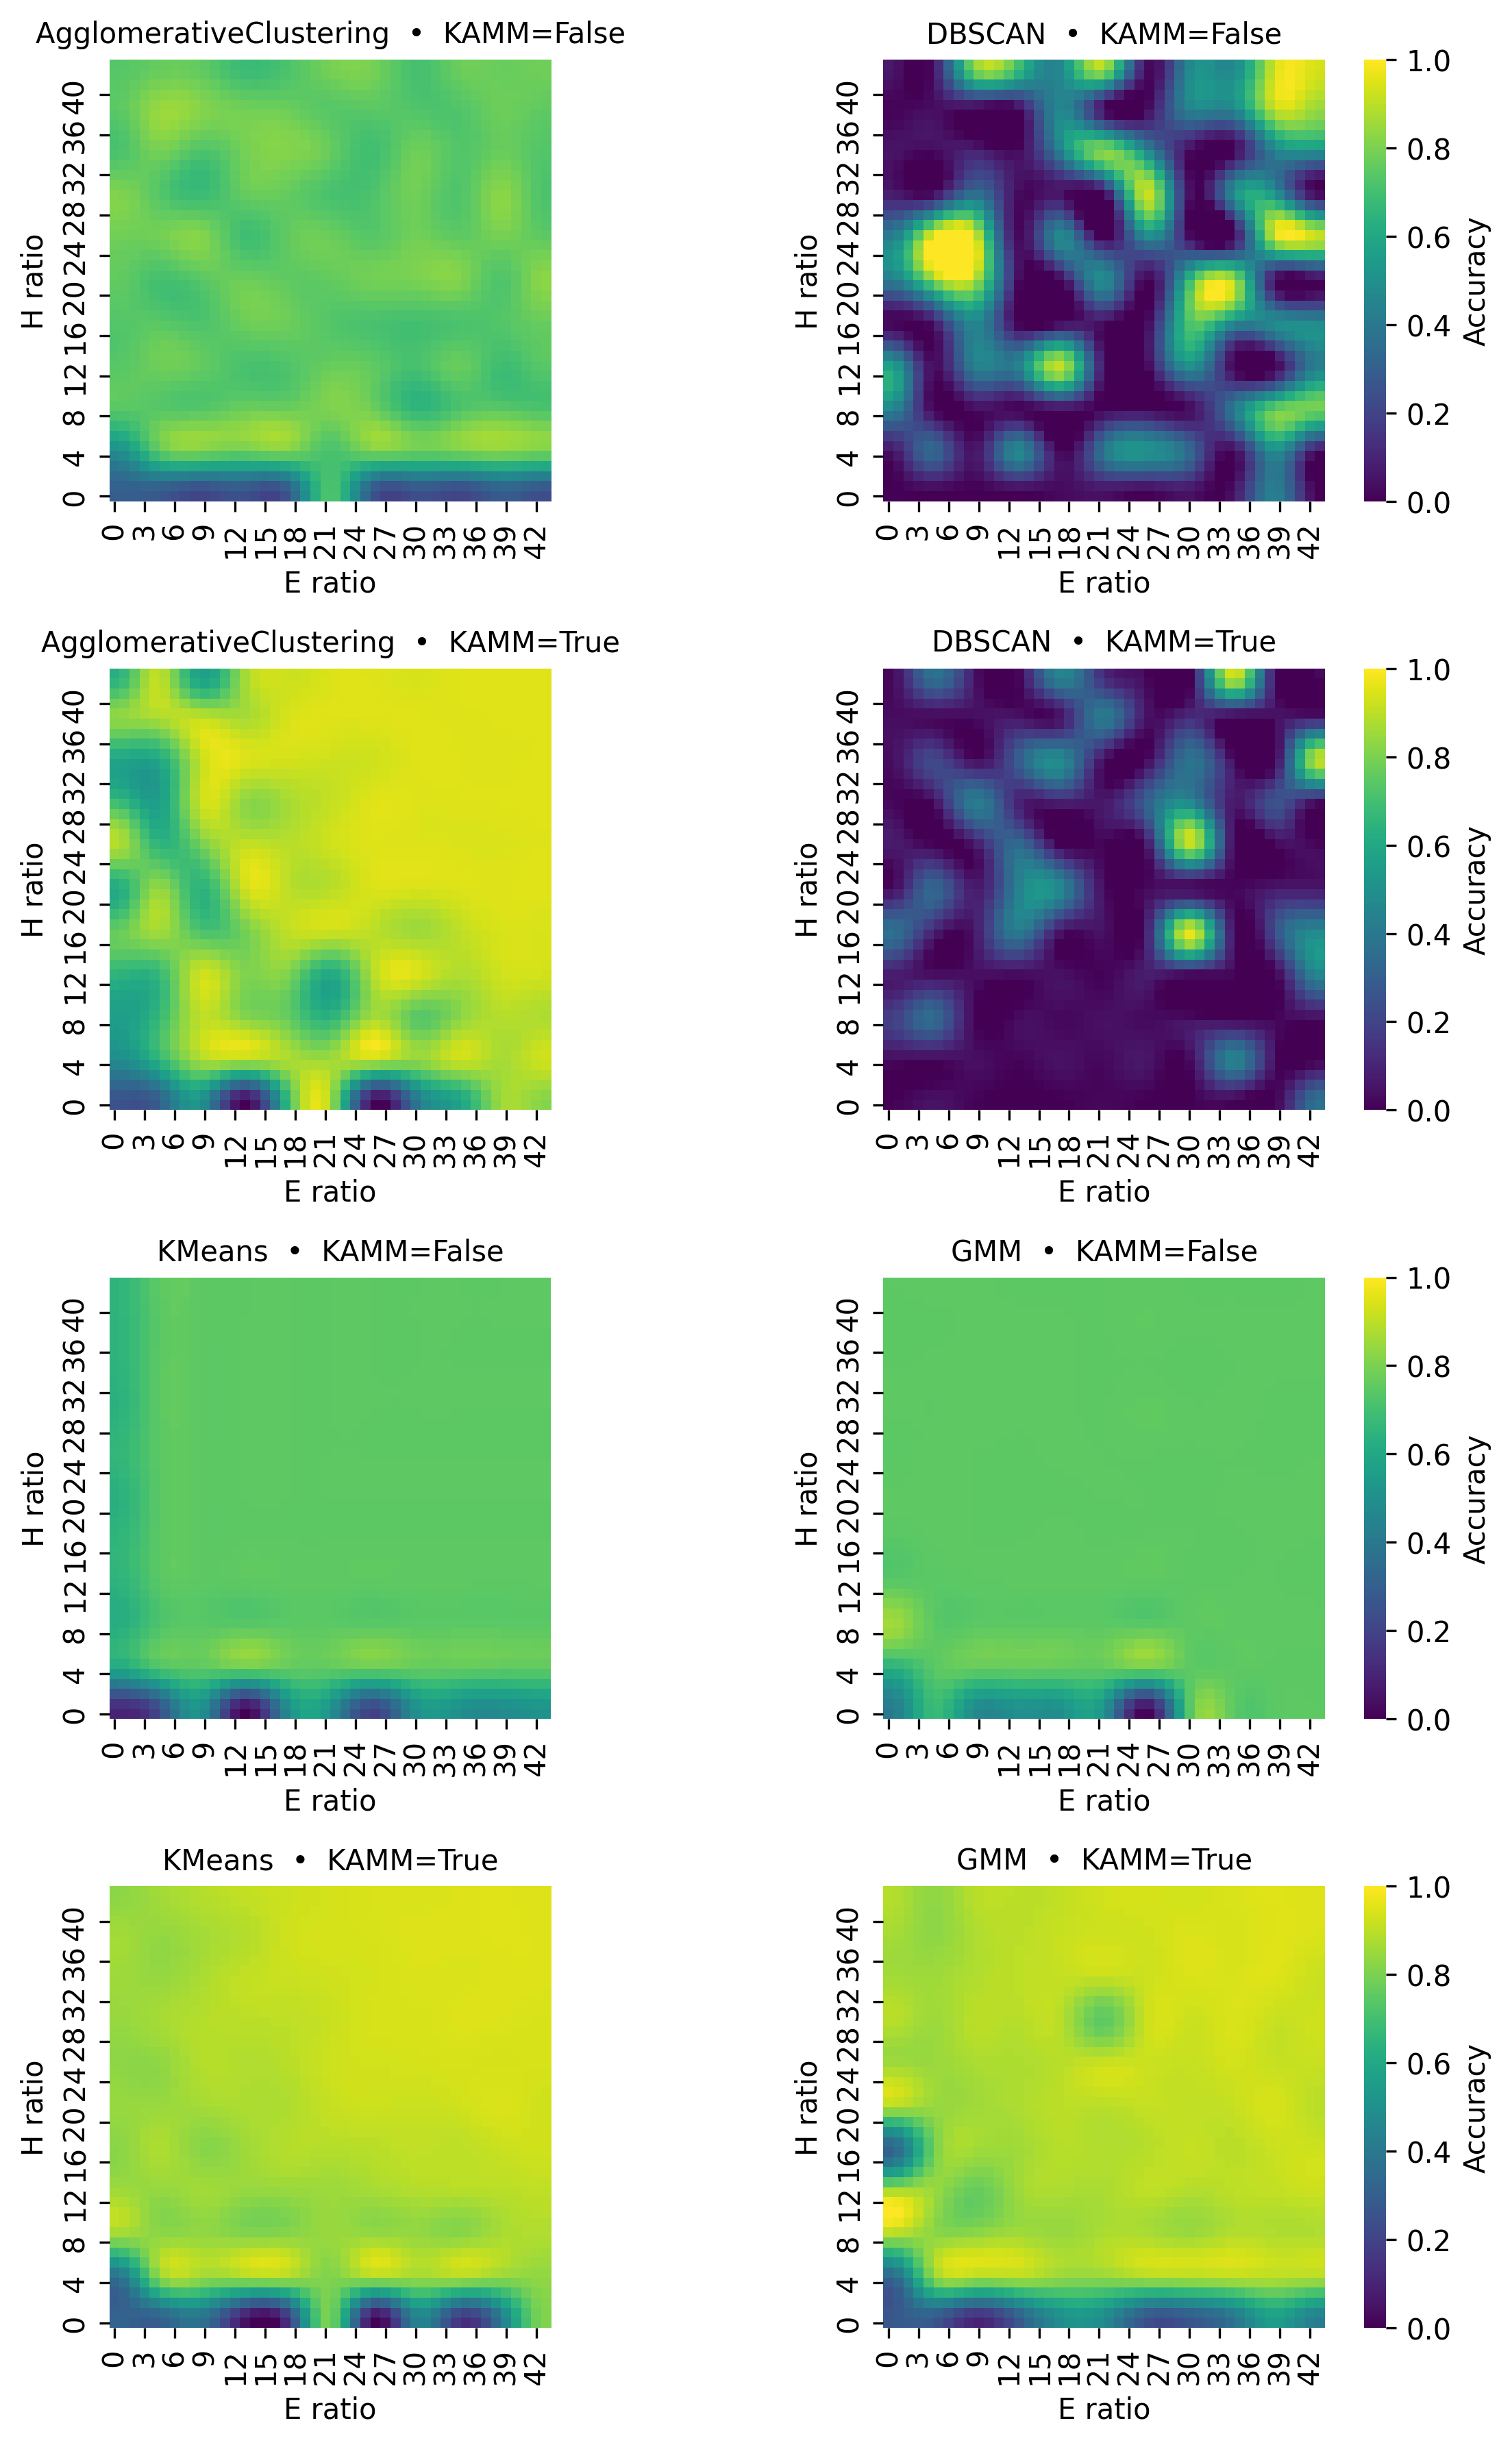
\includegraphics[width=0.7\textwidth]{pictures/accuracy_matrix.png}
\caption{Three-dimensional accuracy maps showing pixel-level clustering accuracy as a function of both hardness contrast ($H_\mathrm{ratio}$) and elastic modulus contrast ($E_\mathrm{ratio}$) for the different clustering algorithms. These maps provide the full contrast-dependent behavior, from which the averaged 2D profiles in Fig.~\ref{fig:kamm_accuracy_comparison} are derived.}
\label{fig:accuracy_matrix}
\end{figure}

\begin{figure}[htbp]
\centering

% --- Row 1 ---
\begin{minipage}{0.45\textwidth}
    \subfloat[Agglomerative Clustering]{
        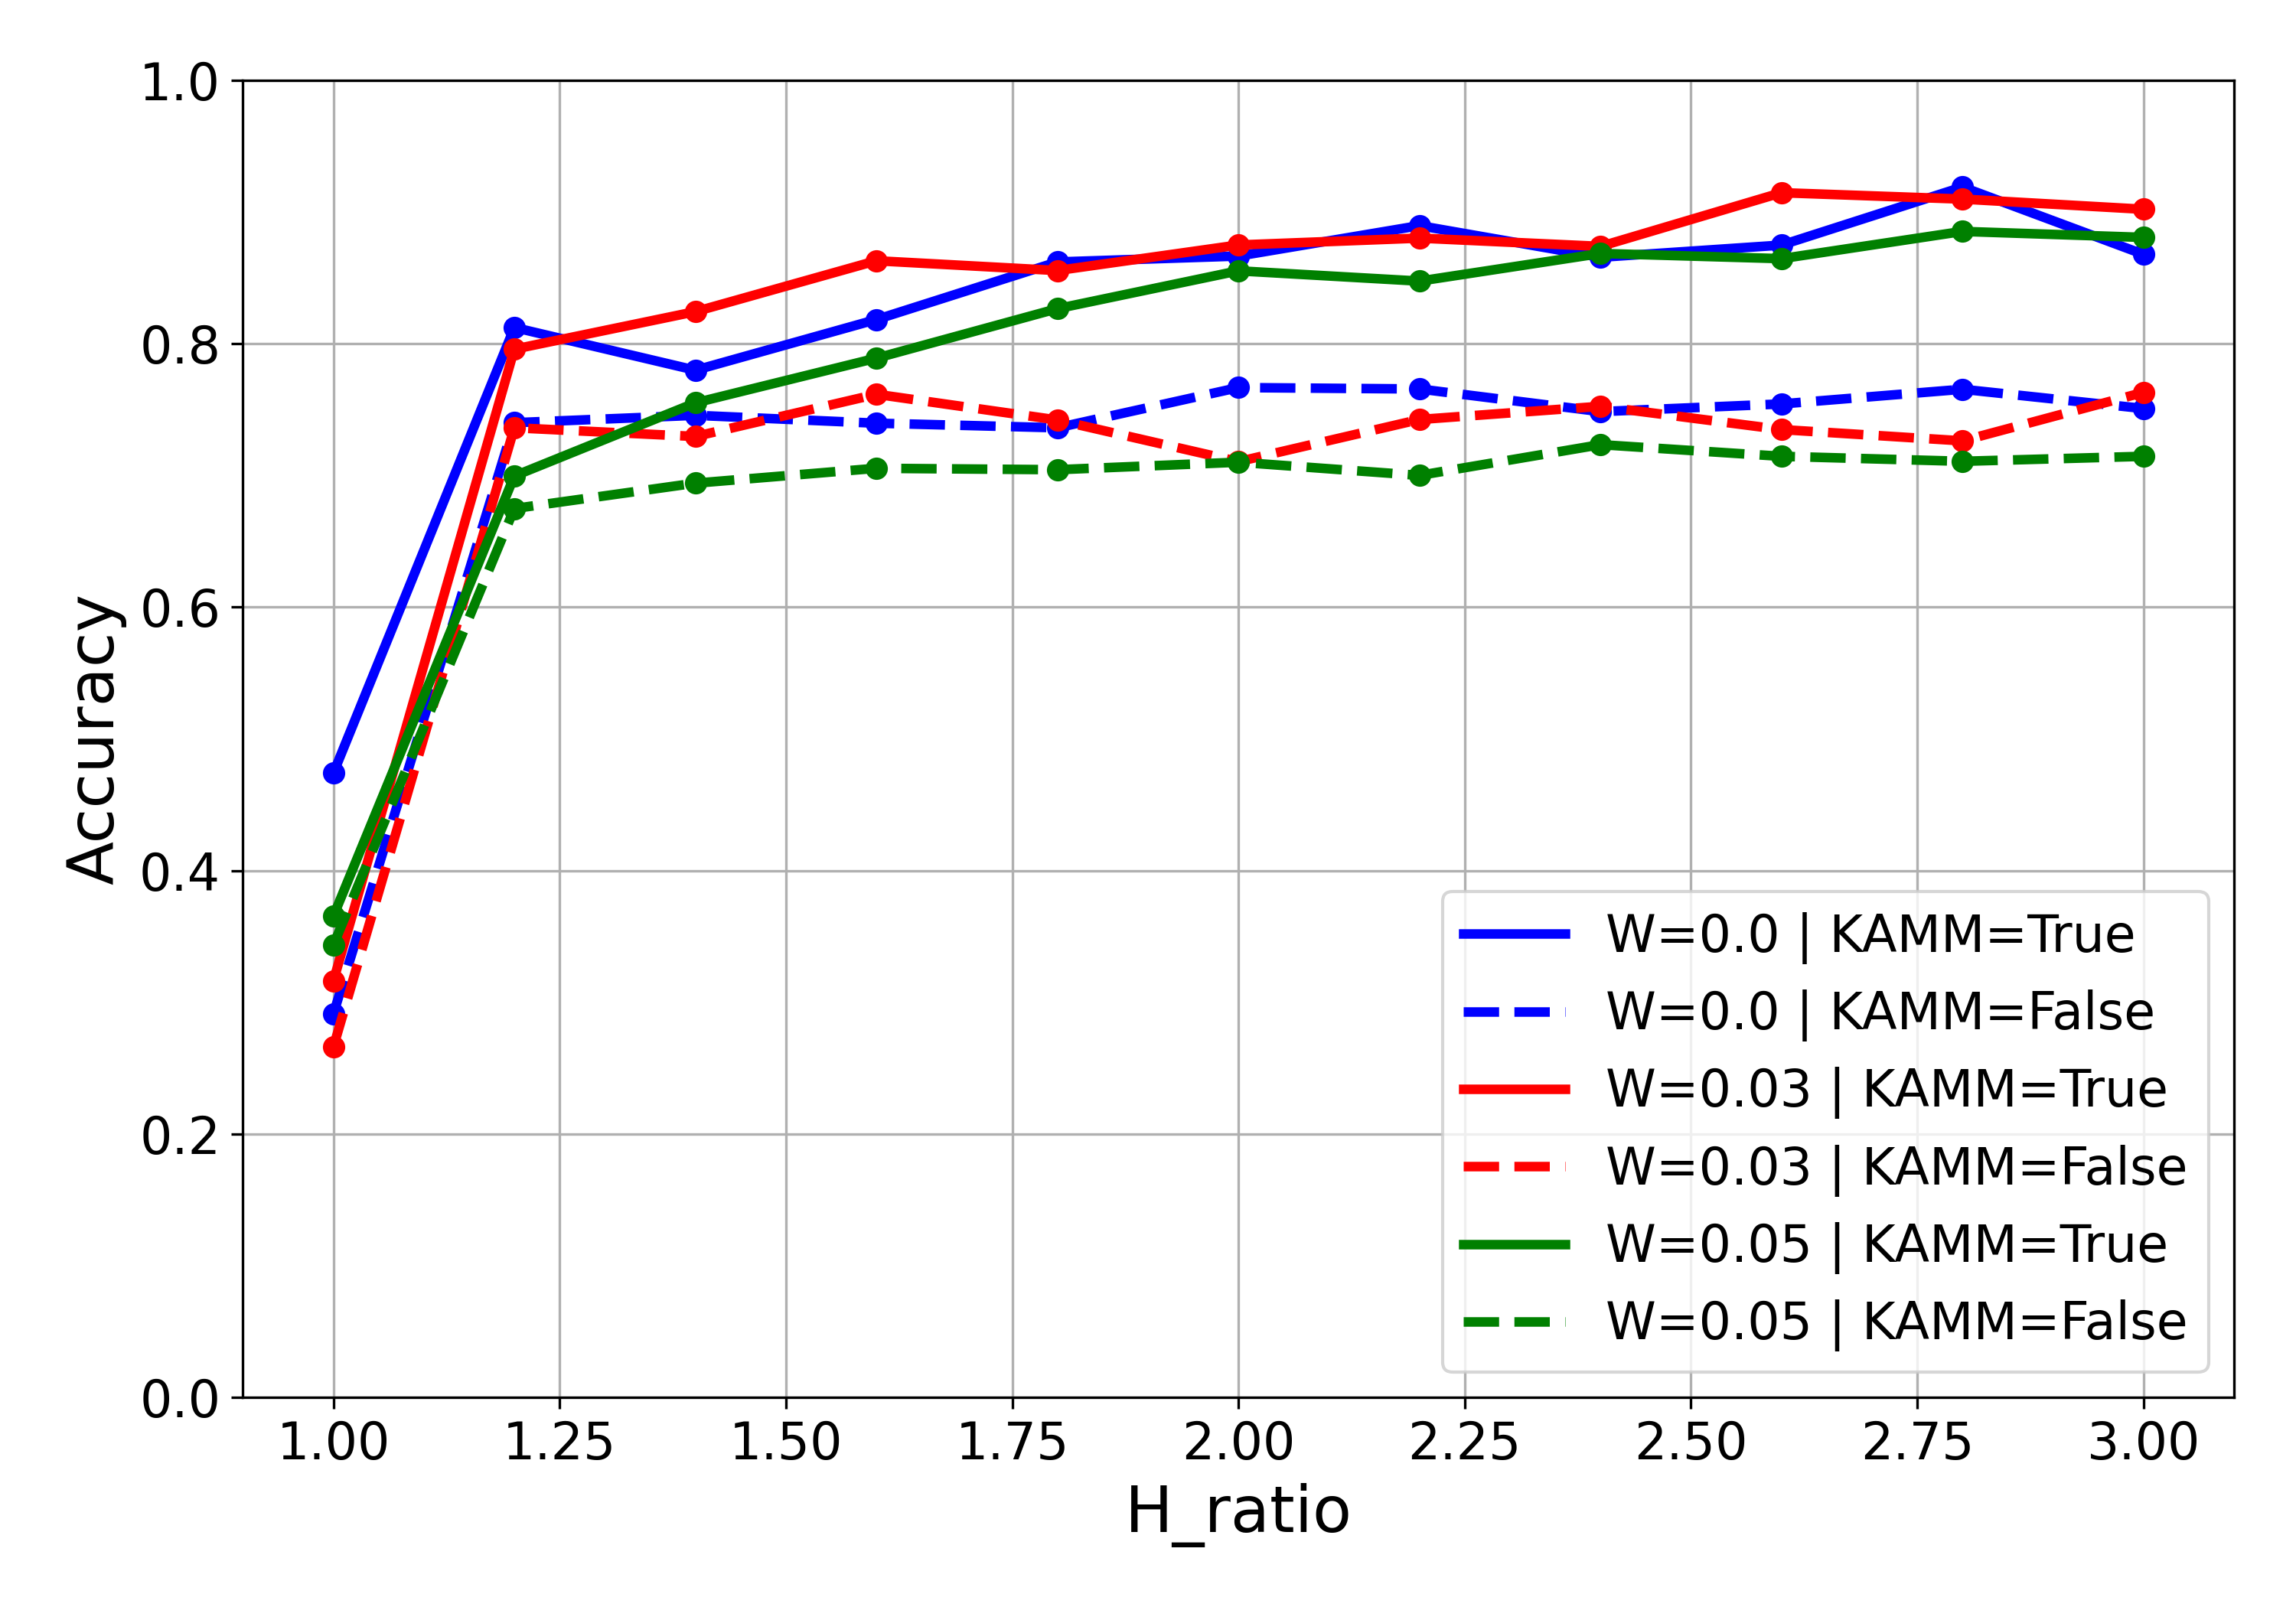
\includegraphics[width=\linewidth]{pictures/Accuracy_MultiSpecimen_AgglomerativeClustering.png}
    }
\end{minipage}
\hfill
\begin{minipage}{0.45\textwidth}
    \subfloat[DBSCAN]{
        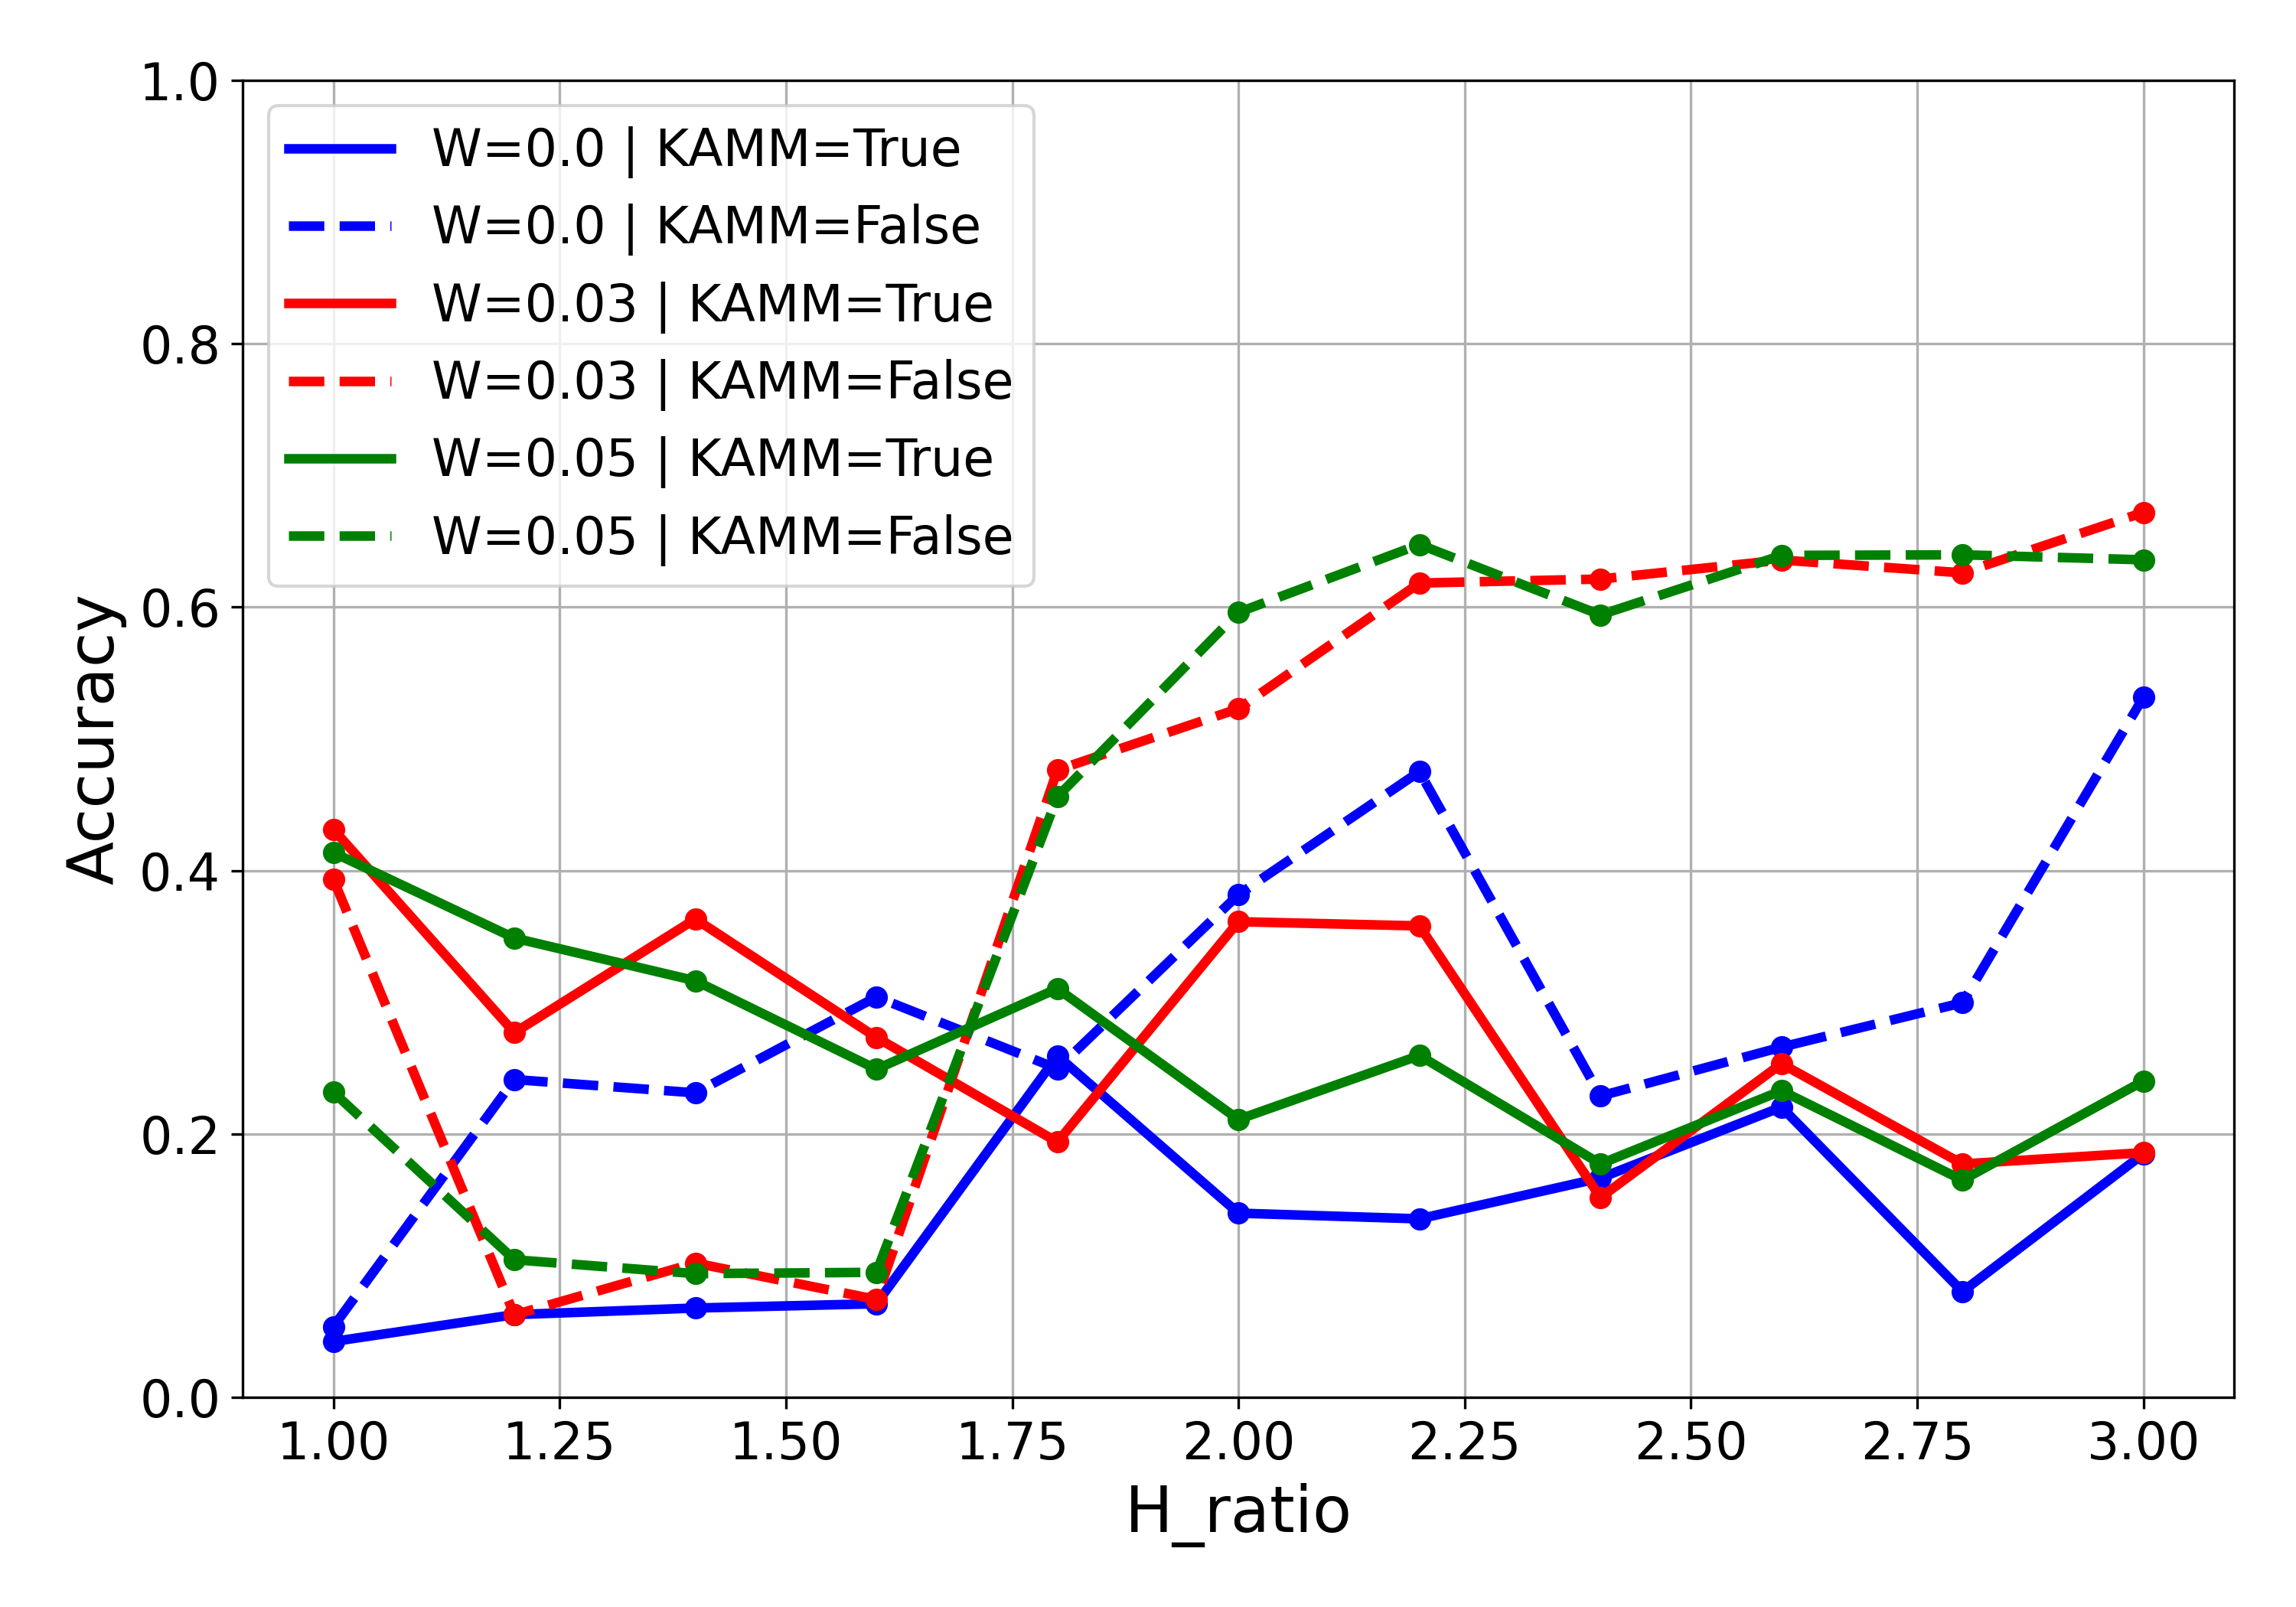
\includegraphics[width=\linewidth]{pictures/Accuracy_MultiSpecimen_DBSCAN.png}
    }
\end{minipage}

\vspace{0.3cm}

% --- Row 2 ---
\begin{minipage}{0.45\textwidth}
    \subfloat[GMM]{
        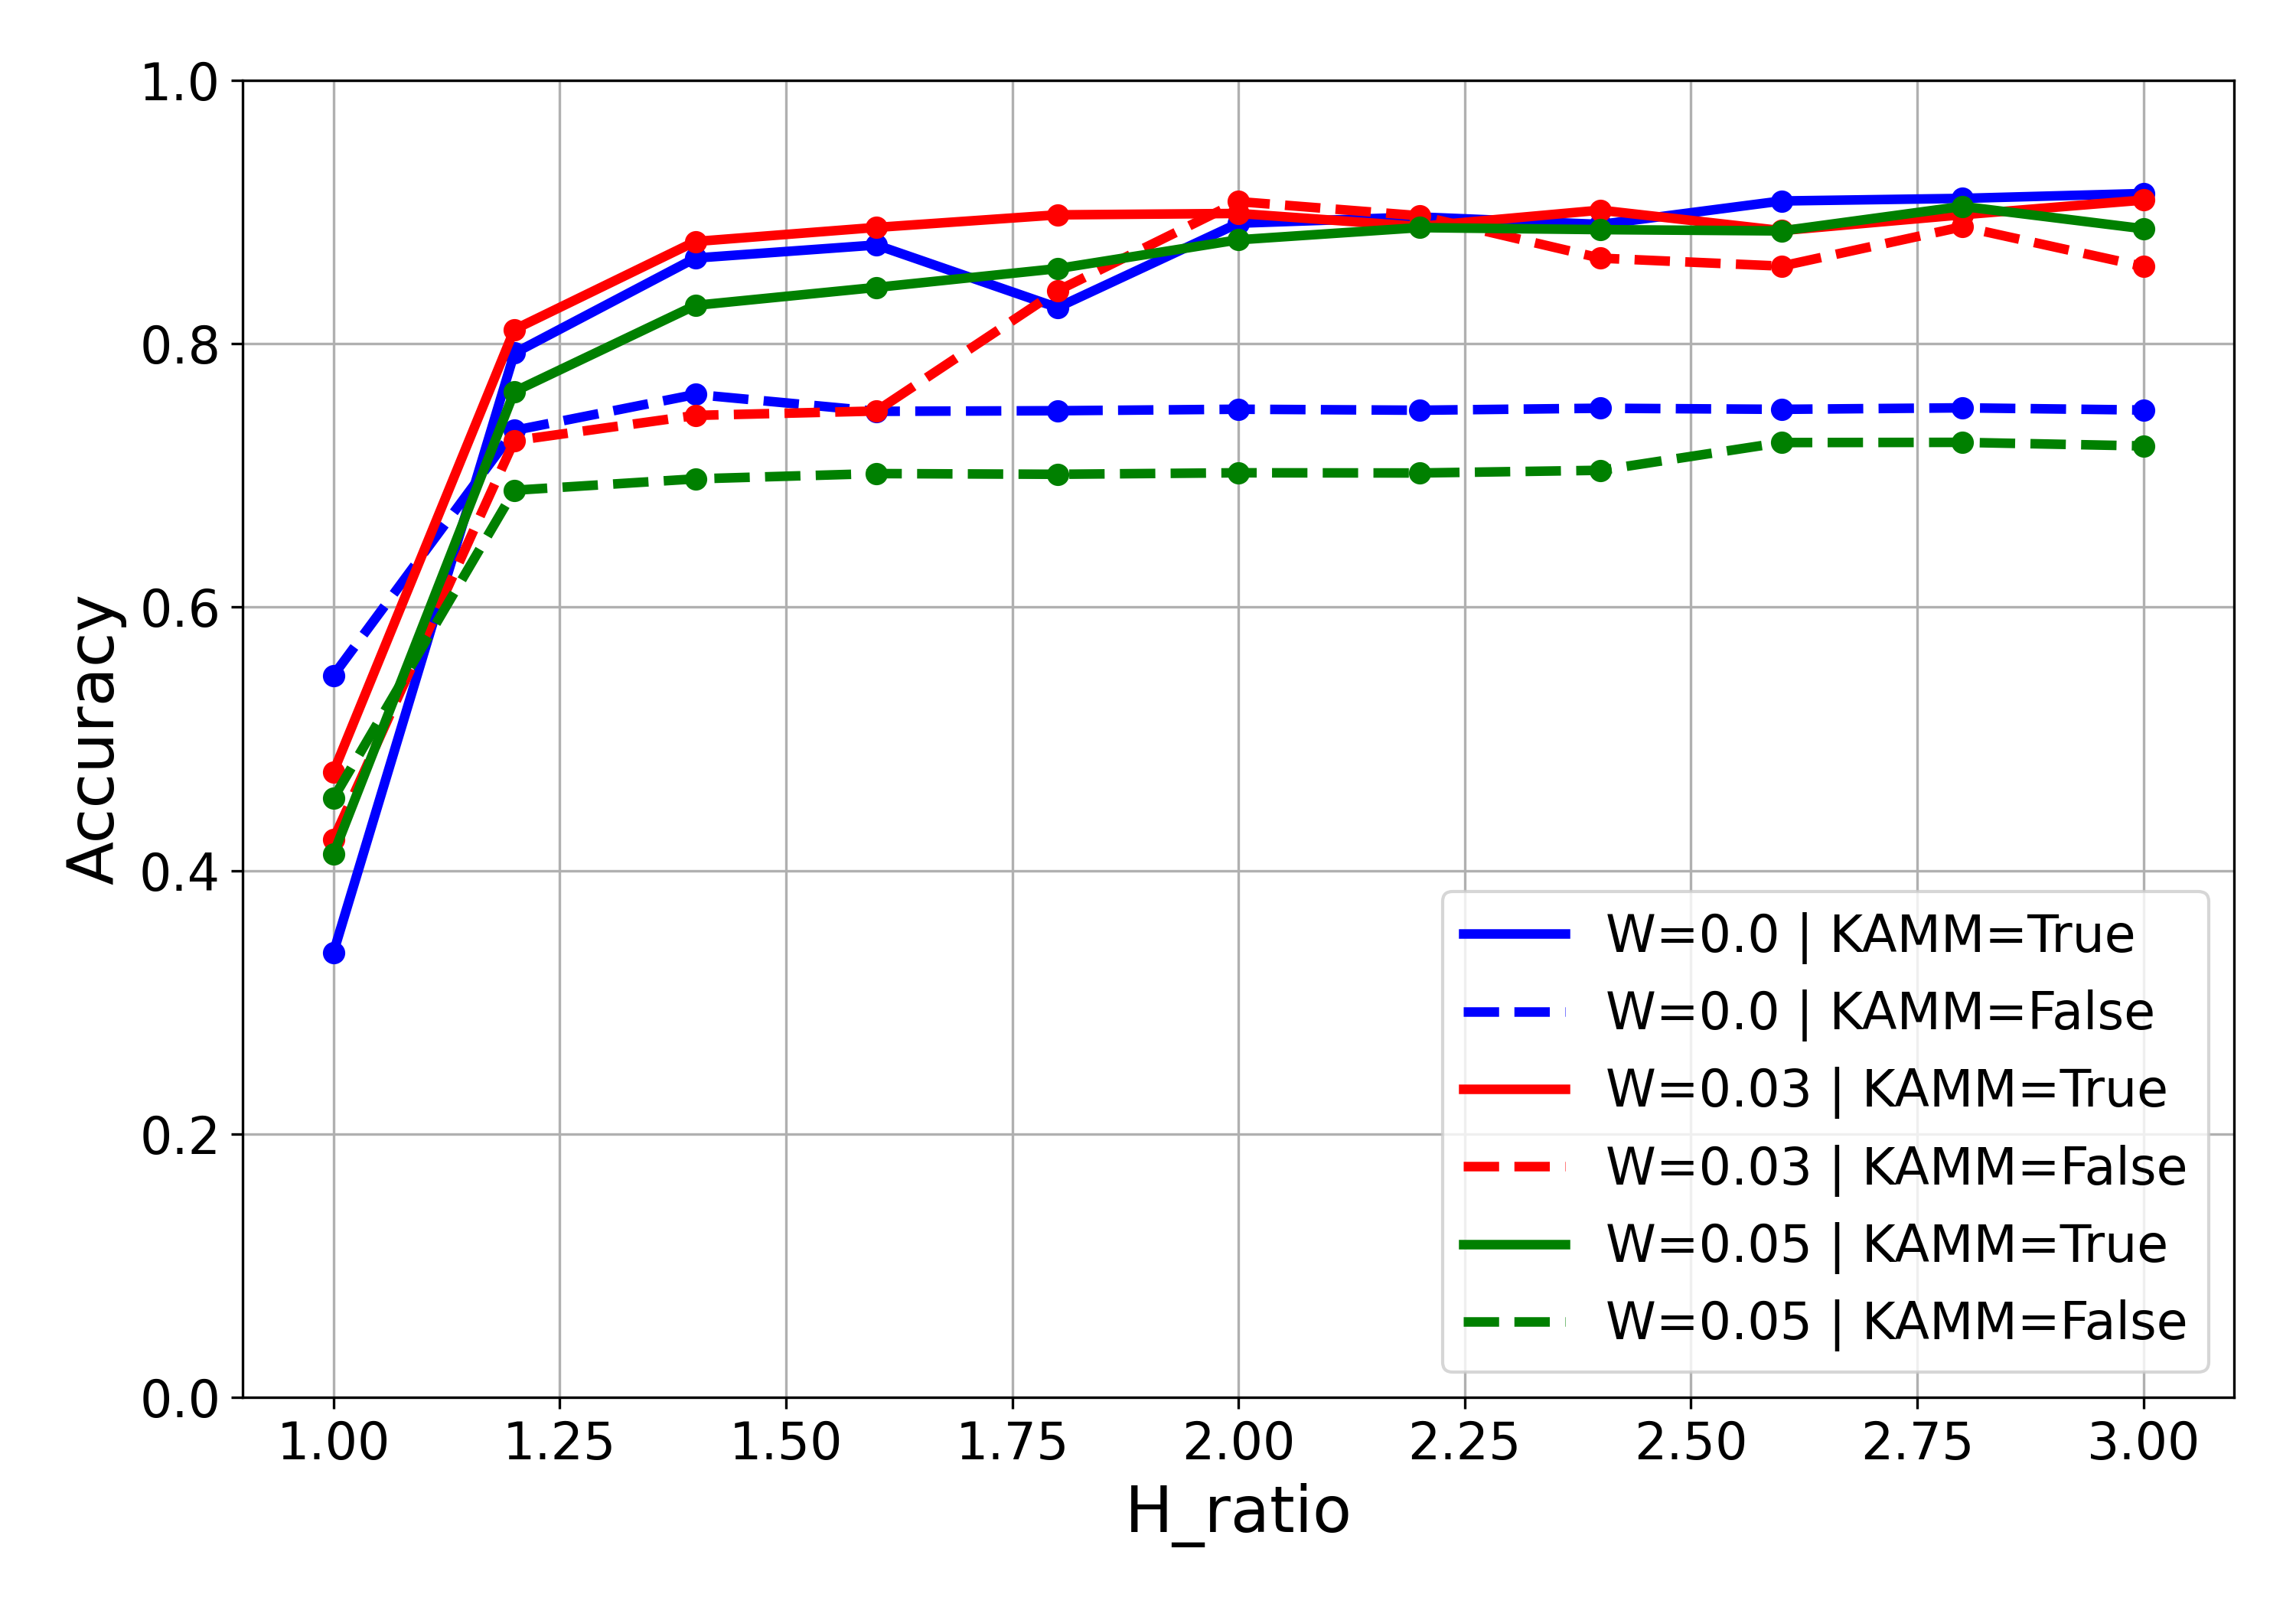
\includegraphics[width=\linewidth]{pictures/Accuracy_MultiSpecimen_GMM.png}
    }
\end{minipage}
\hfill
\begin{minipage}{0.45\textwidth}
    \subfloat[KMeans]{
        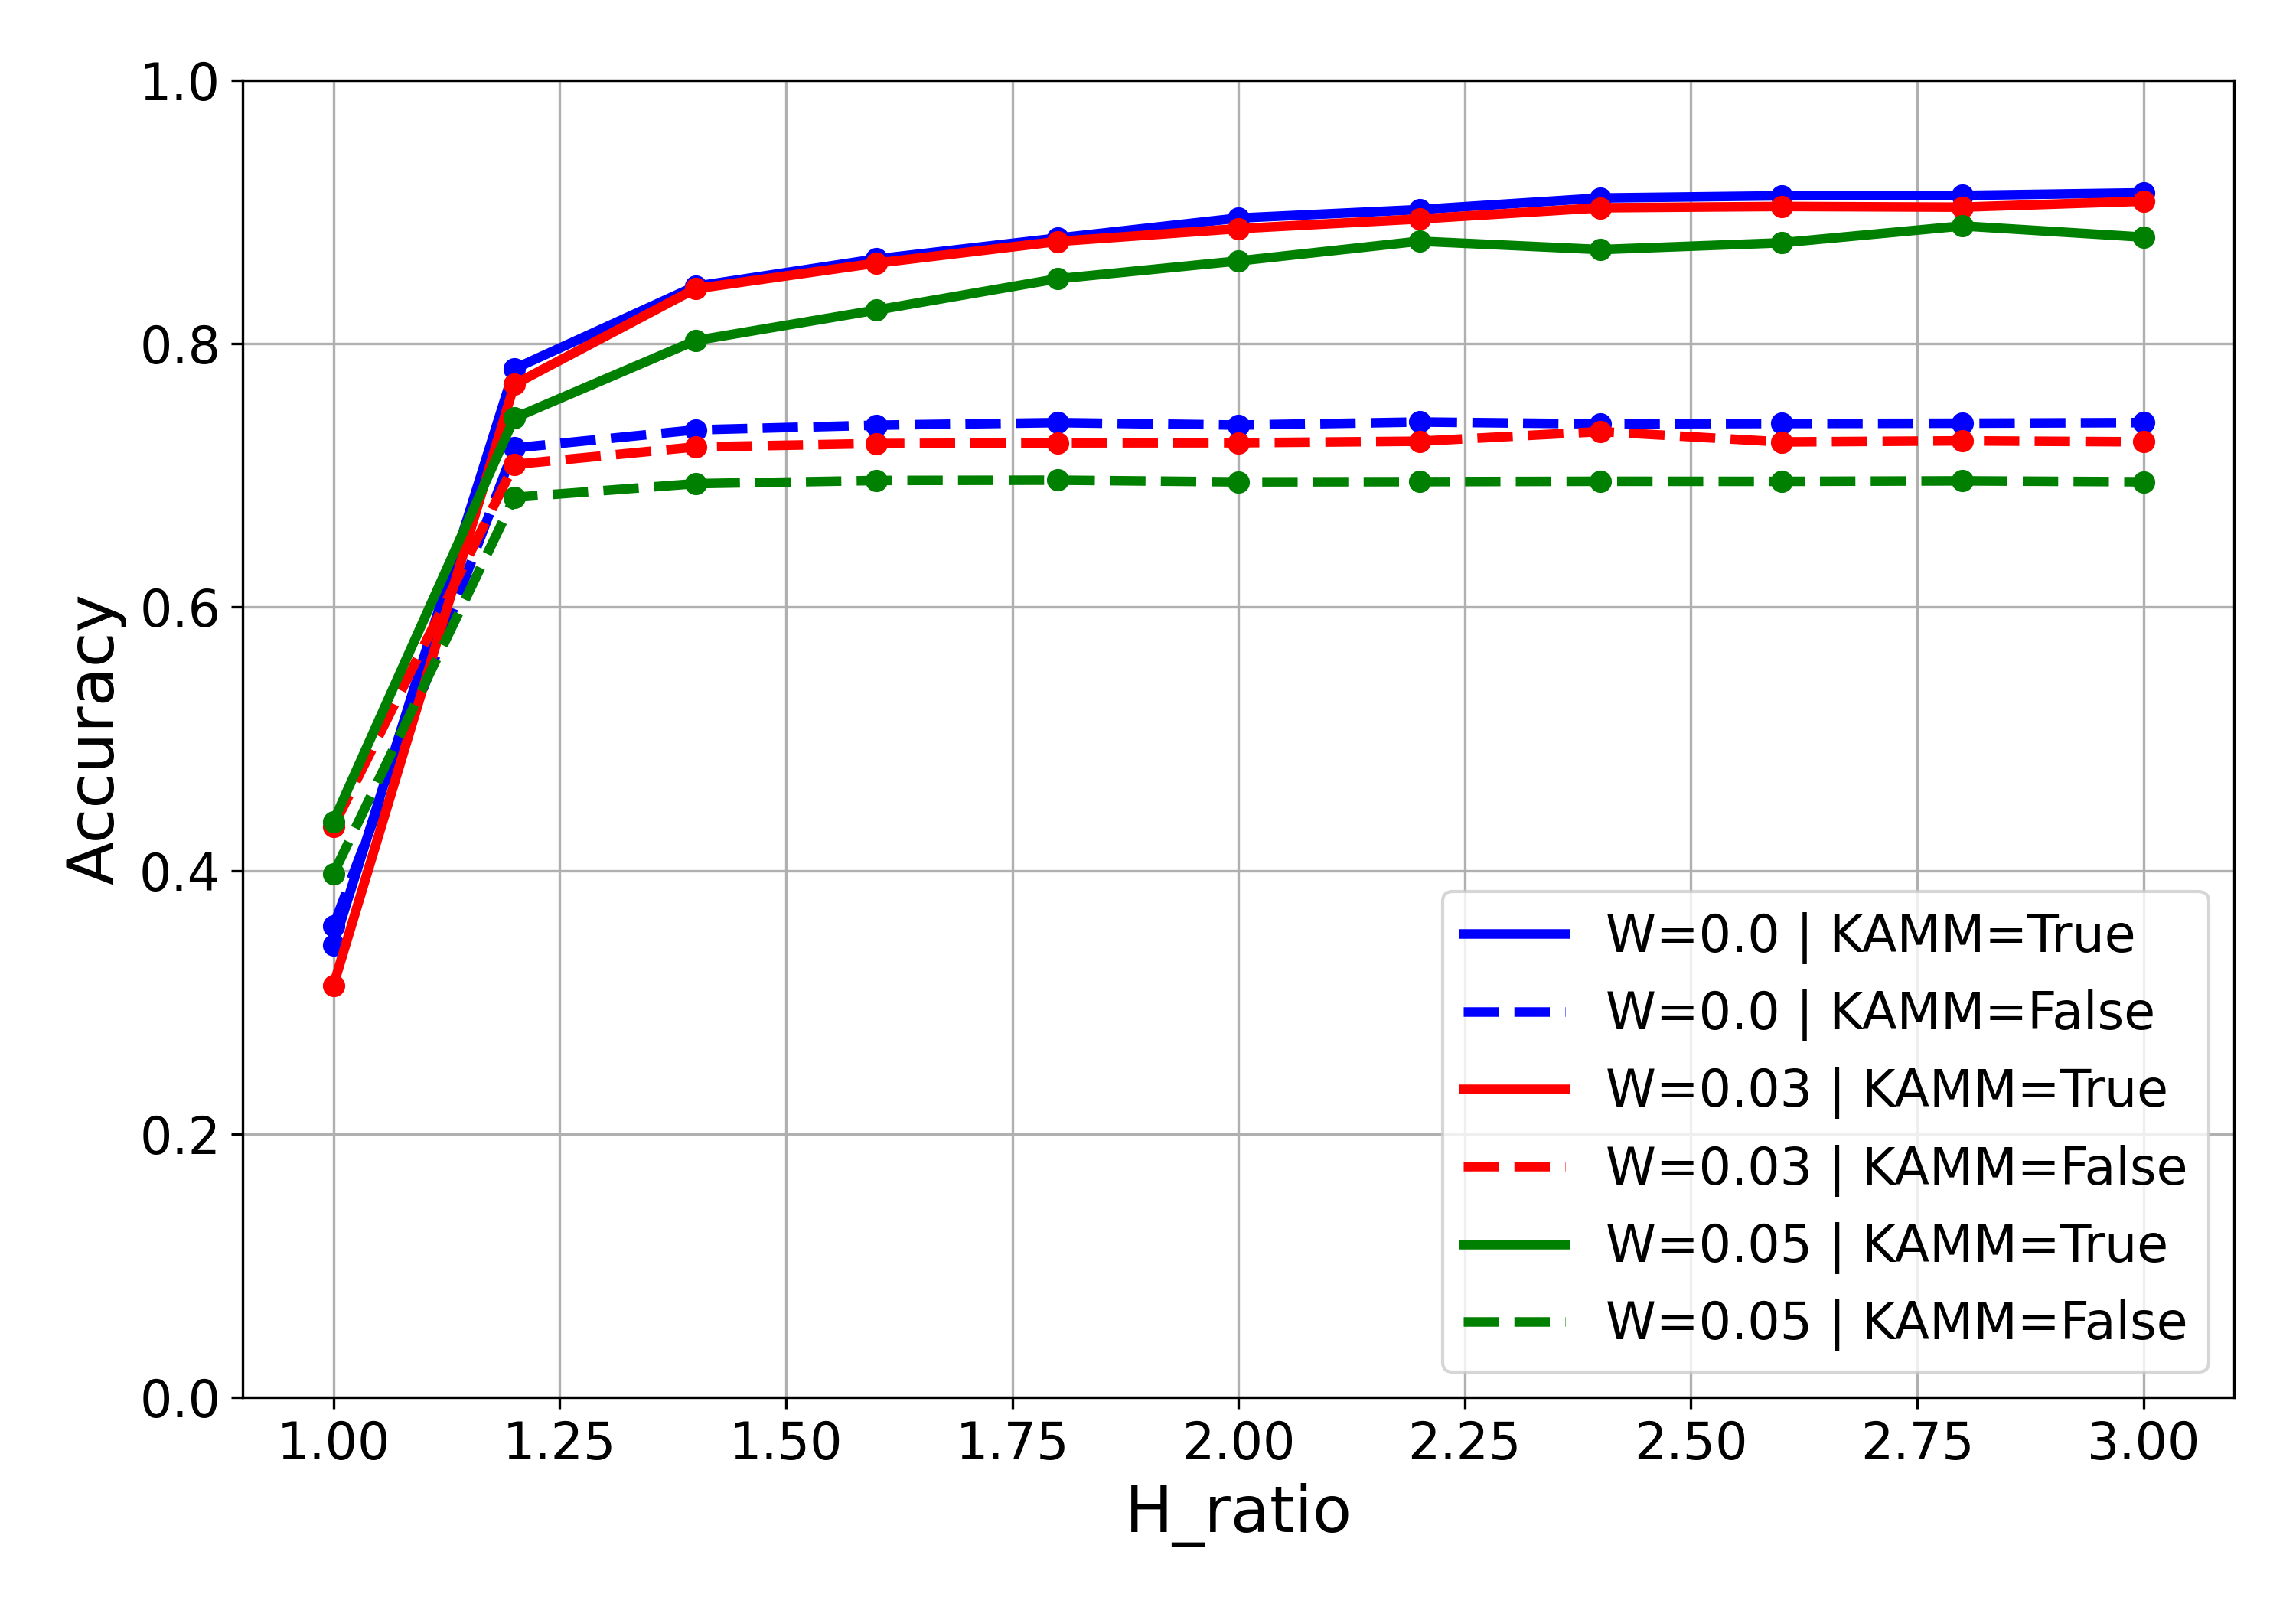
\includegraphics[width=\linewidth]{pictures/Accuracy_MultiSpecimen_KMeans.png}
    }
\end{minipage}

\vspace{0.4cm}

\caption{Pixel-level clustering accuracy as a function of hardness contrast ($H_\mathrm{ratio}$) for the rectangular composite specimen. Solid lines denote clustering with KAMM-based spatial descriptors, whereas dashed lines correspond to baseline clustering using only $(E,H)$ features.}
\label{fig:kamm_accuracy_comparison}
\end{figure}

\subsection{Rectangular composite: effect of noise on clustering accuracy} \label{sec:results_noise}

Figure~\ref{fig:kamm_accuracy_noise} shows the accuracy curves obtained under the noisy condition for the four clustering algorithms considered in this study. Each plot compares the performance with and without the KAMM descriptor for $W=0$ and $W=0.05$.

\begin{figure}[htbp]
\centering

% --- Row 1 ---
\begin{minipage}{0.45\textwidth}
    \subfloat[Agglomerative Clustering]{
        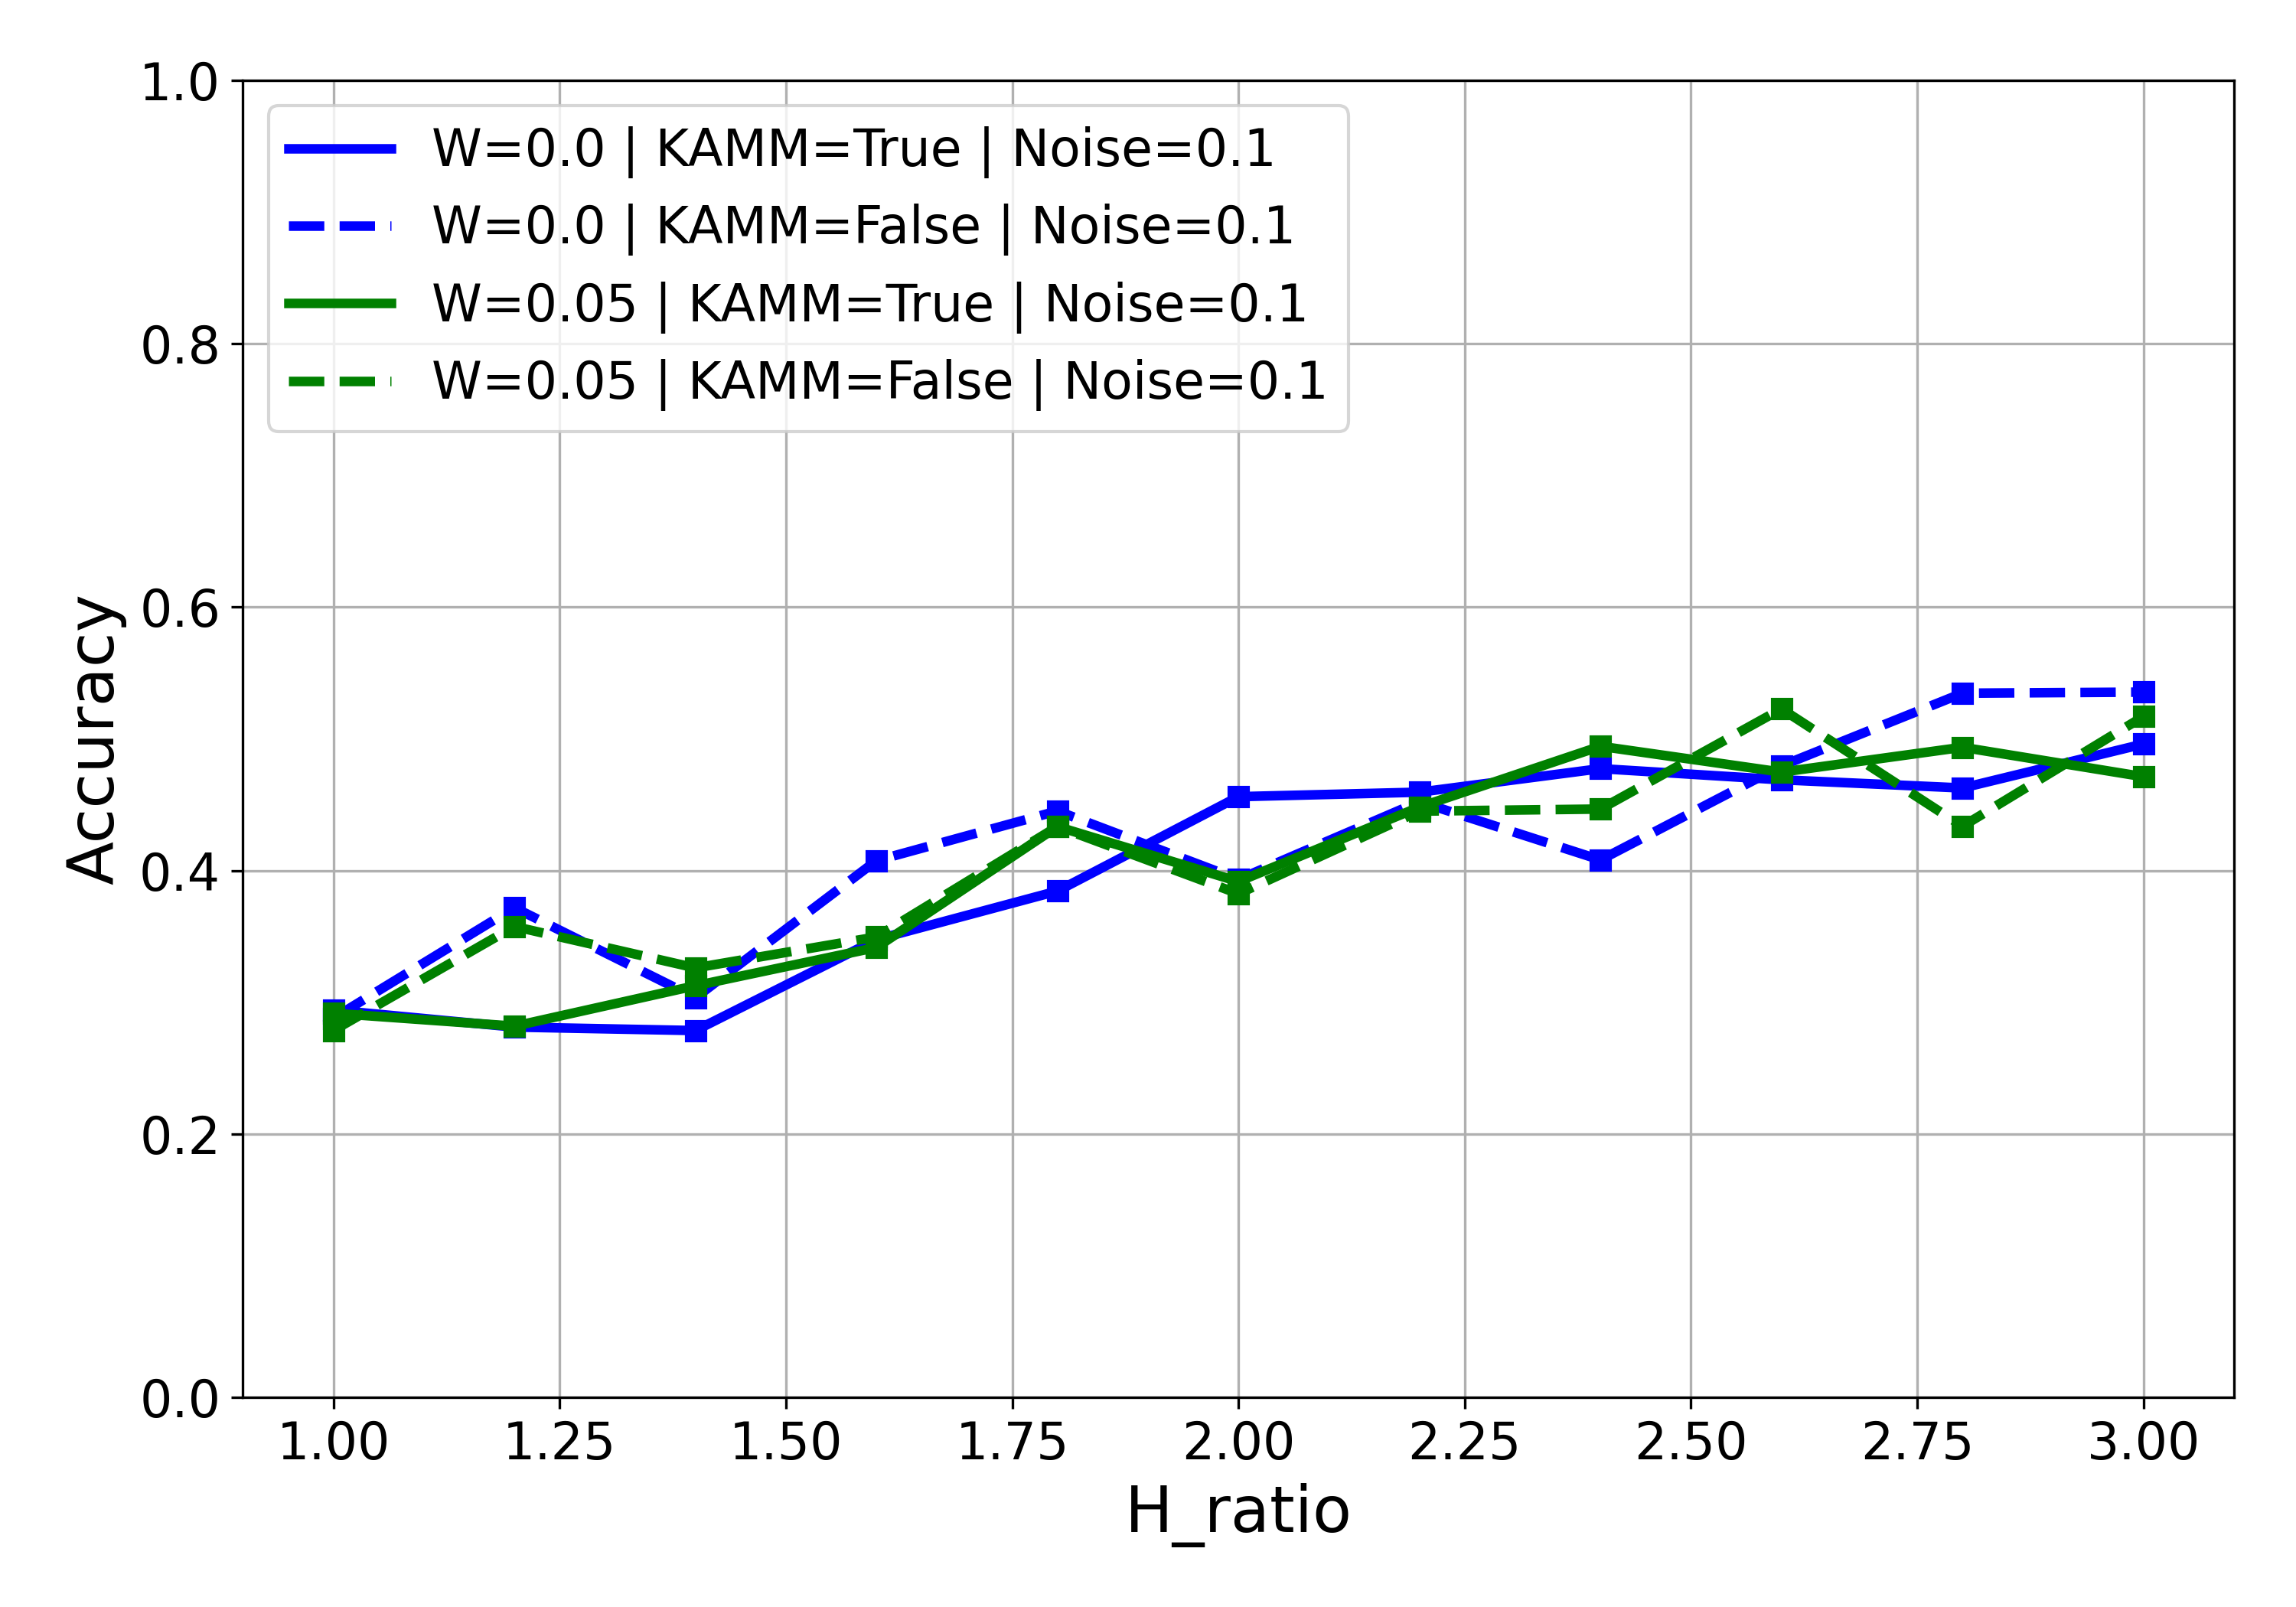
\includegraphics[width=\linewidth]{pictures/Accuracy_MultiSpecimen_AgglomerativeClustering_Noise0.1.png}
    }
\end{minipage}
\hfill
\begin{minipage}{0.45\textwidth}
    \subfloat[DBSCAN]{
        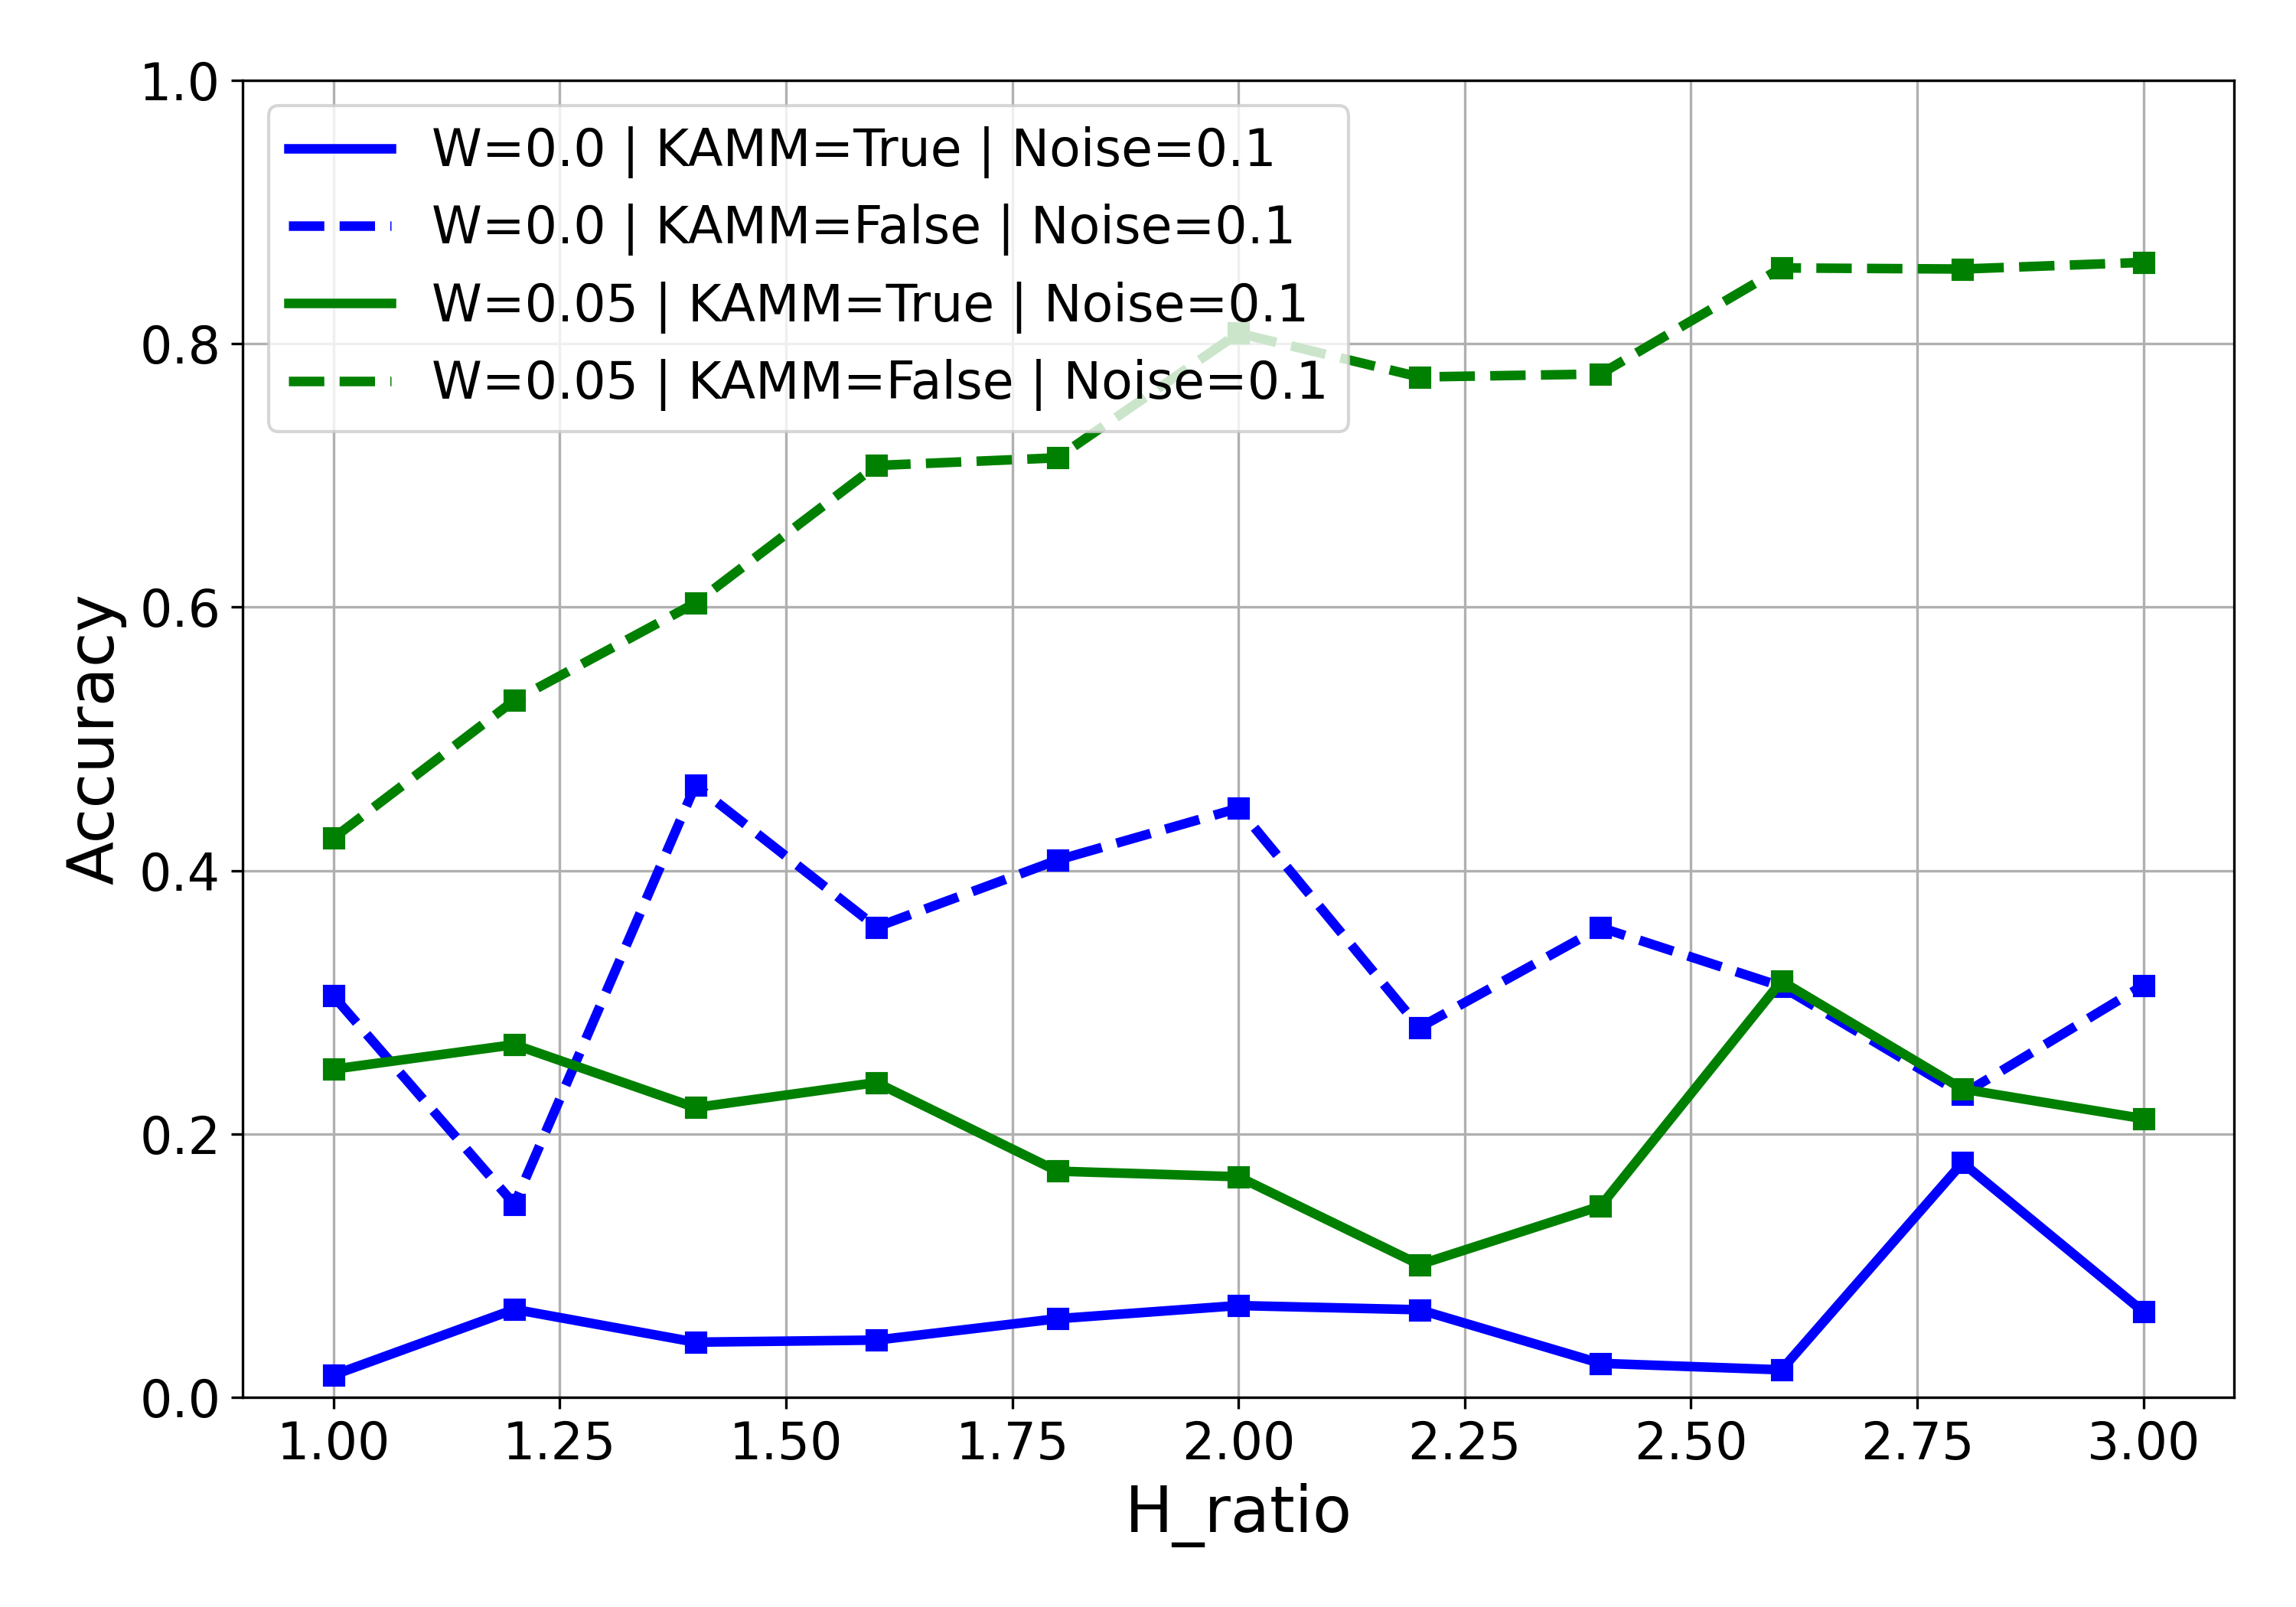
\includegraphics[width=\linewidth]{pictures/Accuracy_MultiSpecimen_DBSCAN_Noise0.1.png}
   }
\end{minipage}

\vspace{0.3cm}

% --- Row 2 ---
\begin{minipage}{0.45\textwidth}
    \subfloat[GMM]{
        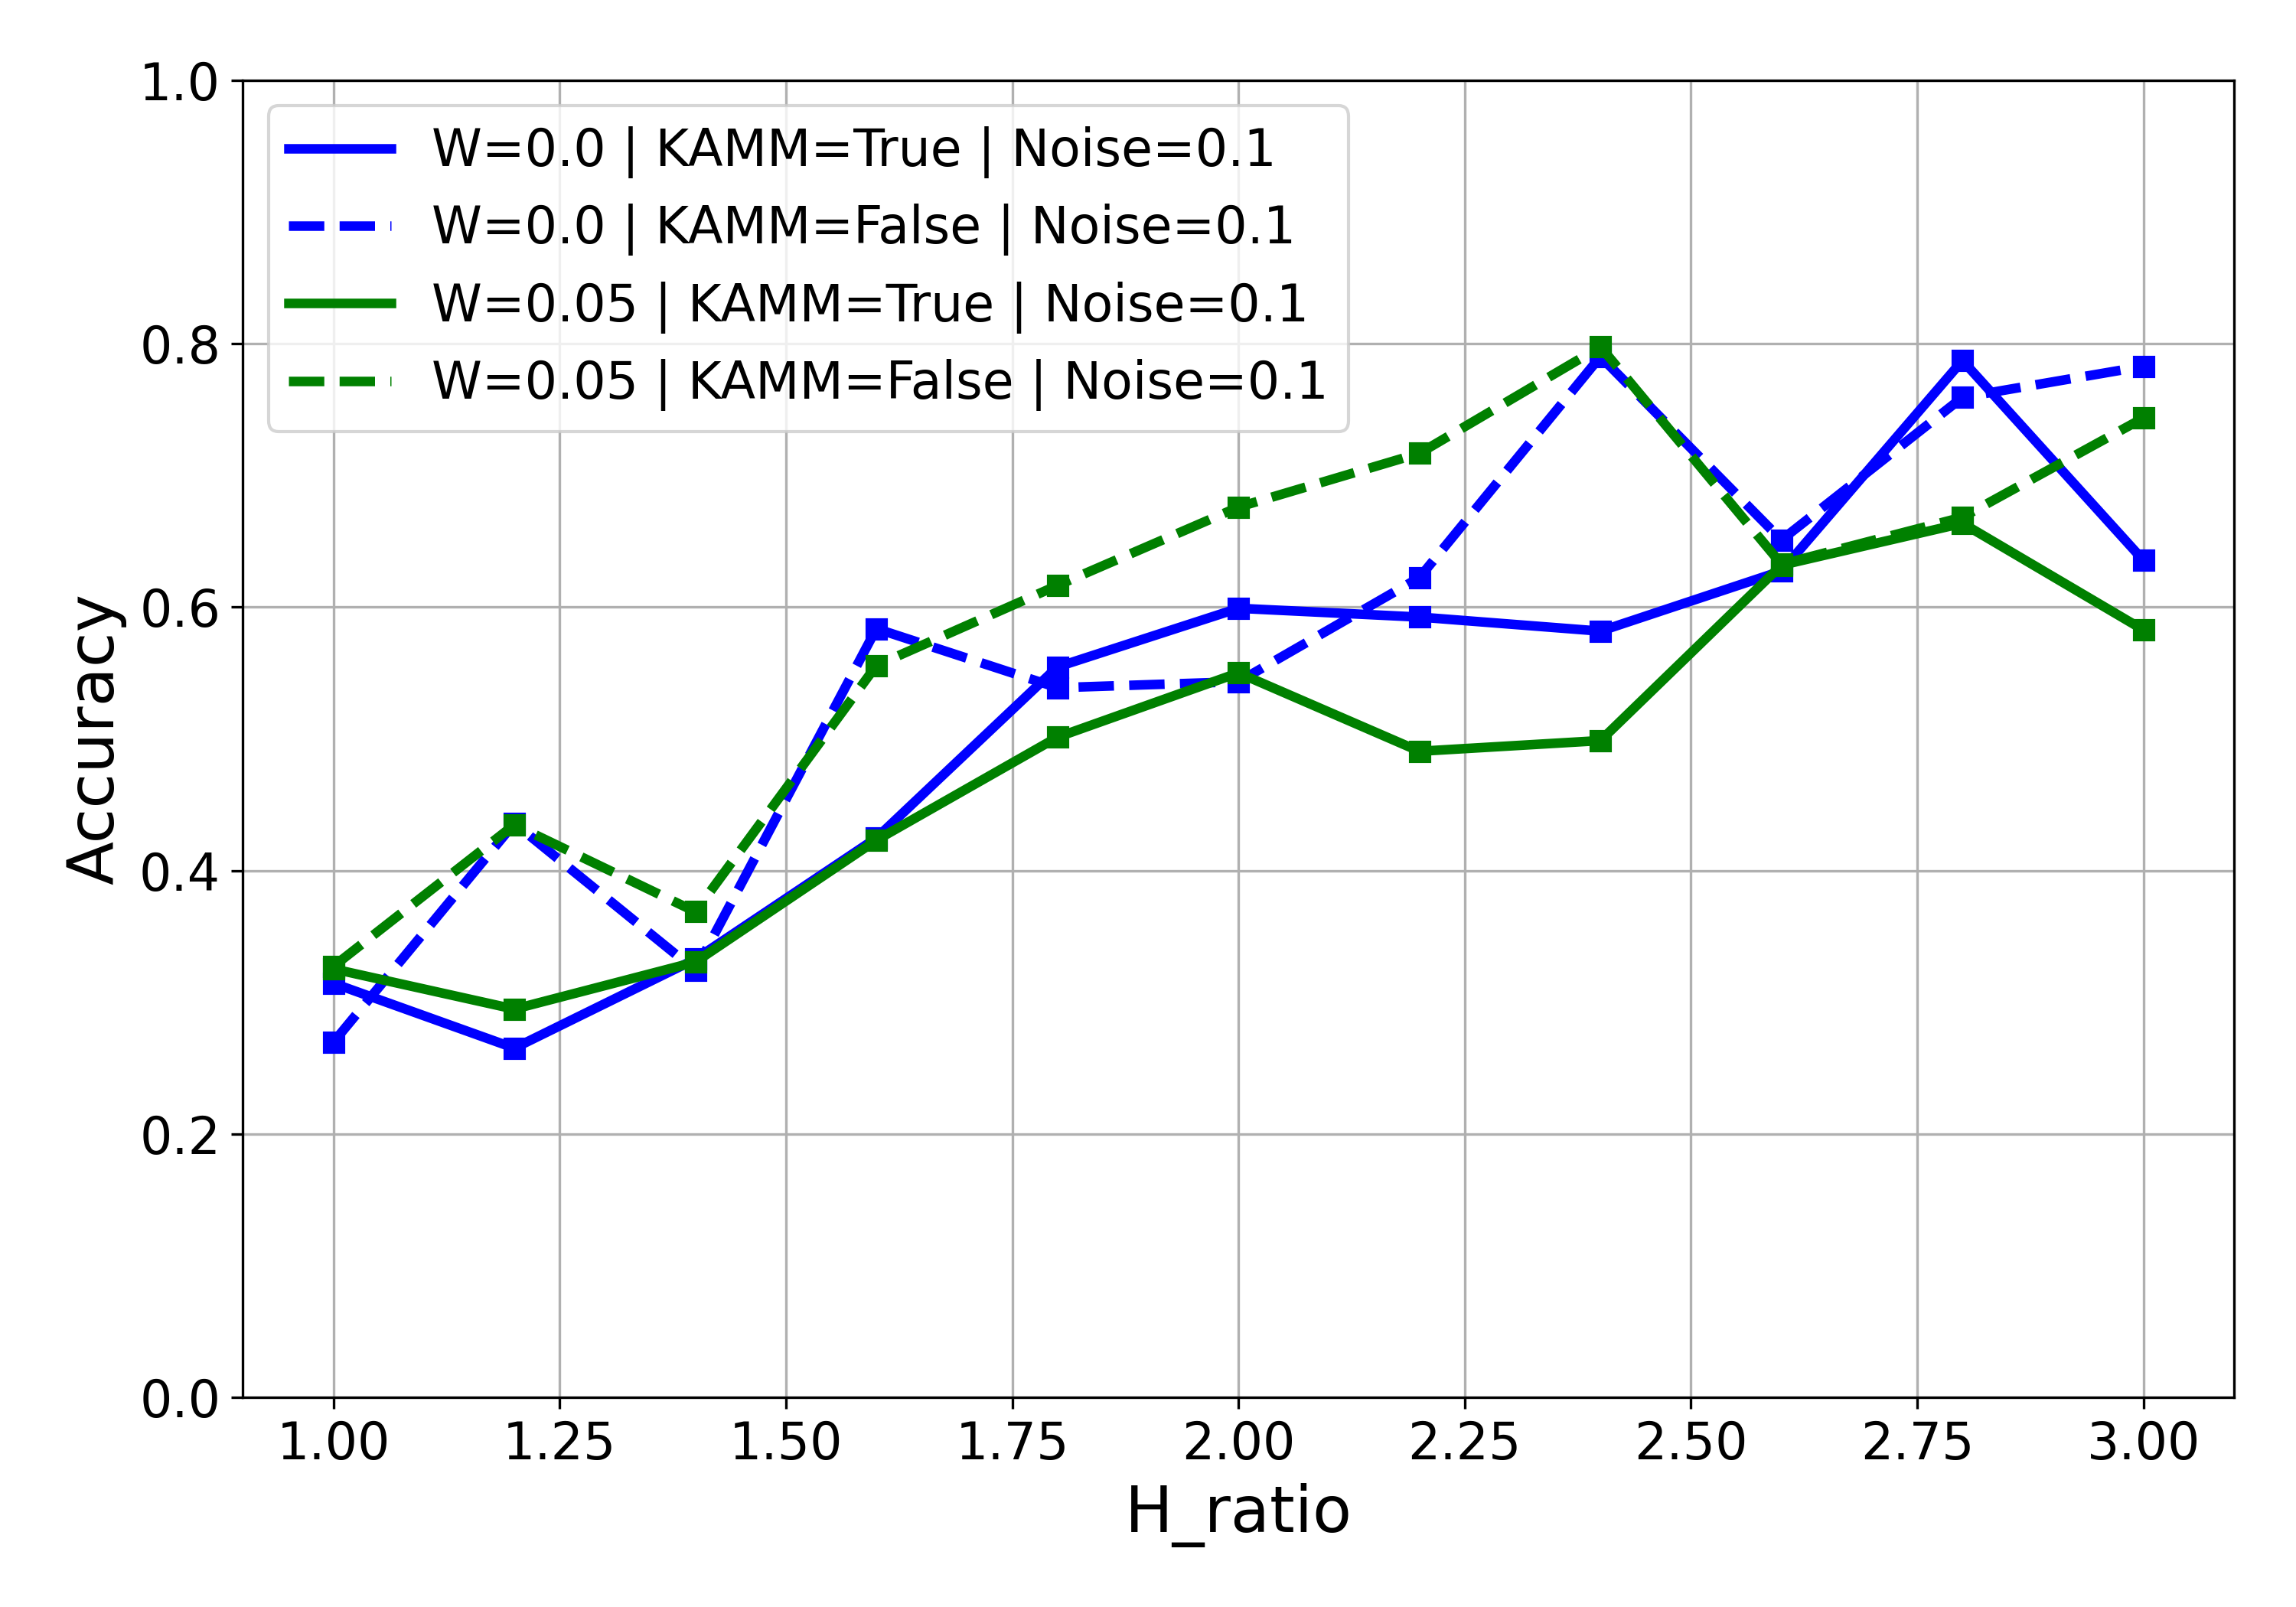
\includegraphics[width=\linewidth]{pictures/Accuracy_MultiSpecimen_GMM_Noise0.1.png}
    }
\end{minipage}
\hfill
\begin{minipage}{0.45\textwidth}
    \subfloat[KMeans]{
        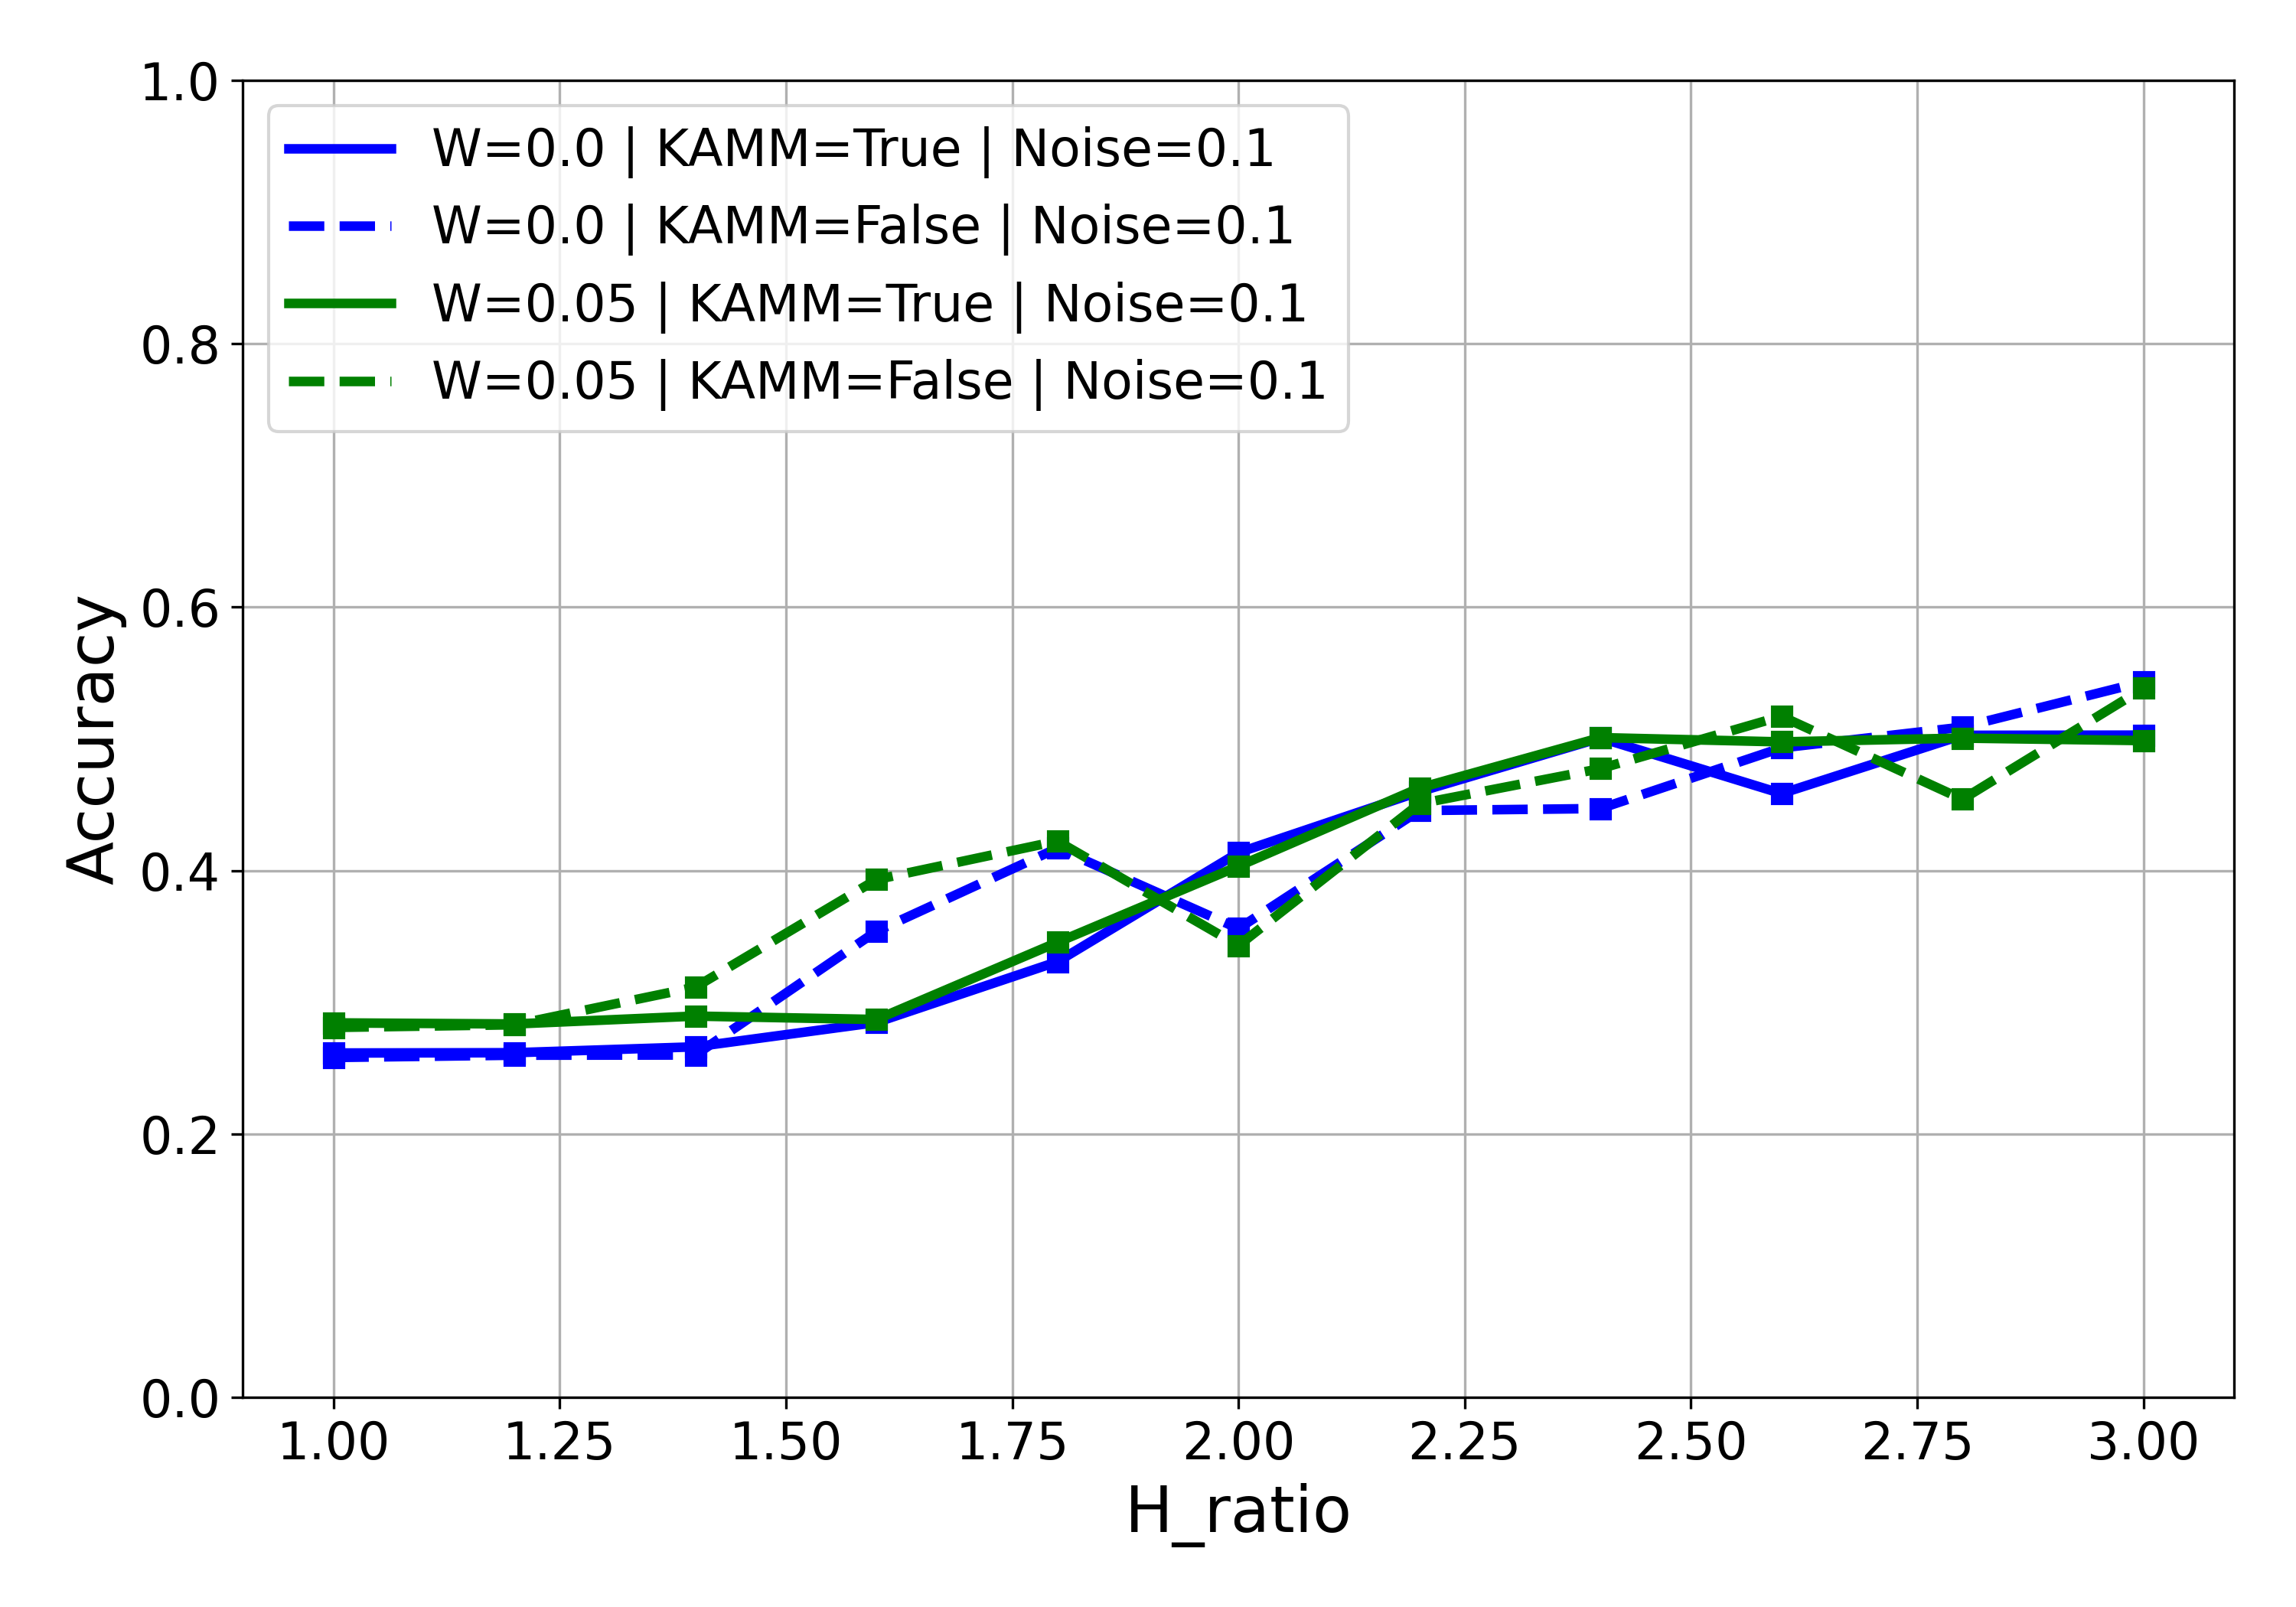
\includegraphics[width=\linewidth]{pictures/Accuracy_MultiSpecimen_KMeans_Noise0.1.png}
    }
\end{minipage}

\vspace{0.4cm}

\caption{Pixel-level clustering accuracy vs.\ hardness contrast ($H_\mathrm{ratio}$) for the rectangular composite specimen with 10\% synthetic noise added. Solid lines: clustering with KAMM; dashed lines: baseline $(E,H)$-only clustering.}
\label{fig:kamm_accuracy_noise}
\end{figure}

For the Agglomerative clustering method, the introduction of noise leads to a drastic loss of accuracy across all $H$ ratios. Moreover, the curves obtained with and without KAMM are nearly indistinguishable, indicating that KAMM provides no measurable benefit under noisy conditions. The method appears highly sensitive to perturbations and rapidly loses meaningful clustering capability when noise is present. For DBSCAN, the behavior differs markedly. In the presence of noise, DBSCAN generally performs better without KAMM across most contrast ratios, particularly when the interphase width approaches zero. The inclusion of the KAMM descriptor appears to degrade density-based clustering under noisy conditions, likely due to the alteration of local density structure in feature space. For both GMM and KMeans, noise substantially reduces accuracy, and the curves with and without KAMM remain very similar. This suggests that these centroid- and model-based methods become dominated by noise, rendering the contribution of the KAMM descriptor largely ineffective. Their overall accuracy remains significantly lower compared to the noise-free case. Overall, under noisy conditions, the four methods exhibit distinct sensitivities to the KAMM descriptor: Agglomerative clustering, GMM, and KMeans experience strong performance degradation regardless of KAMM, whereas DBSCAN performs more robustly when KAMM is excluded, particularly at low $H$ ratios.

\subsection{Rectangular composite with graded interphase}
\label{sec:results_rectComposite}

Figure~\ref{fig:Clustering_GradedInterphase} presents the pixel-level clustering accuracy as a function of hardness contrast ($H_\mathrm{ratio}$) for the rectangular composite with a graded interphase ($W = 0.03$). The impact of the KAMM descriptor varies significantly across the different clustering algorithms. Agglomerative clustering exhibits a clear improvement when KAMM is included, with consistently higher accuracy across the investigated hardness contrasts. This suggests that hierarchical linkage criteria benefit from the enhanced spatial coherence introduced by the KAMM descriptor in the presence of a diffuse interface. In contrast, DBSCAN shows its lowest performance when KAMM features are incorporated. The density-based formulation appears to be negatively affected by the additional neighborhood-derived information, leading to reduced phase separability compared to the $(E,H)$-only baseline. GMM displays nearly identical performance with and without KAMM, indicating that the probabilistic modeling of the feature distribution is largely insensitive to the added spatial descriptor in this graded configuration. KMeans, on the other hand, demonstrates a noticeable improvement with KAMM, particularly at intermediate and high $H_\mathrm{ratio}$ values. The inclusion of spatial information enhances cluster compactness and phase discrimination for this centroid-based method. Overall, for the graded interphase case, KAMM clearly benefits centroid- and linkage-based approaches (KMeans and Agglomerative), has negligible influence on GMM, and degrades the performance of the density-based DBSCAN algorithm.


\begin{figure}[htbp]
\centering

% --- Row 1 ---
\begin{minipage}{0.45\textwidth}
    \subfloat[Agglomerative Clustering]{
        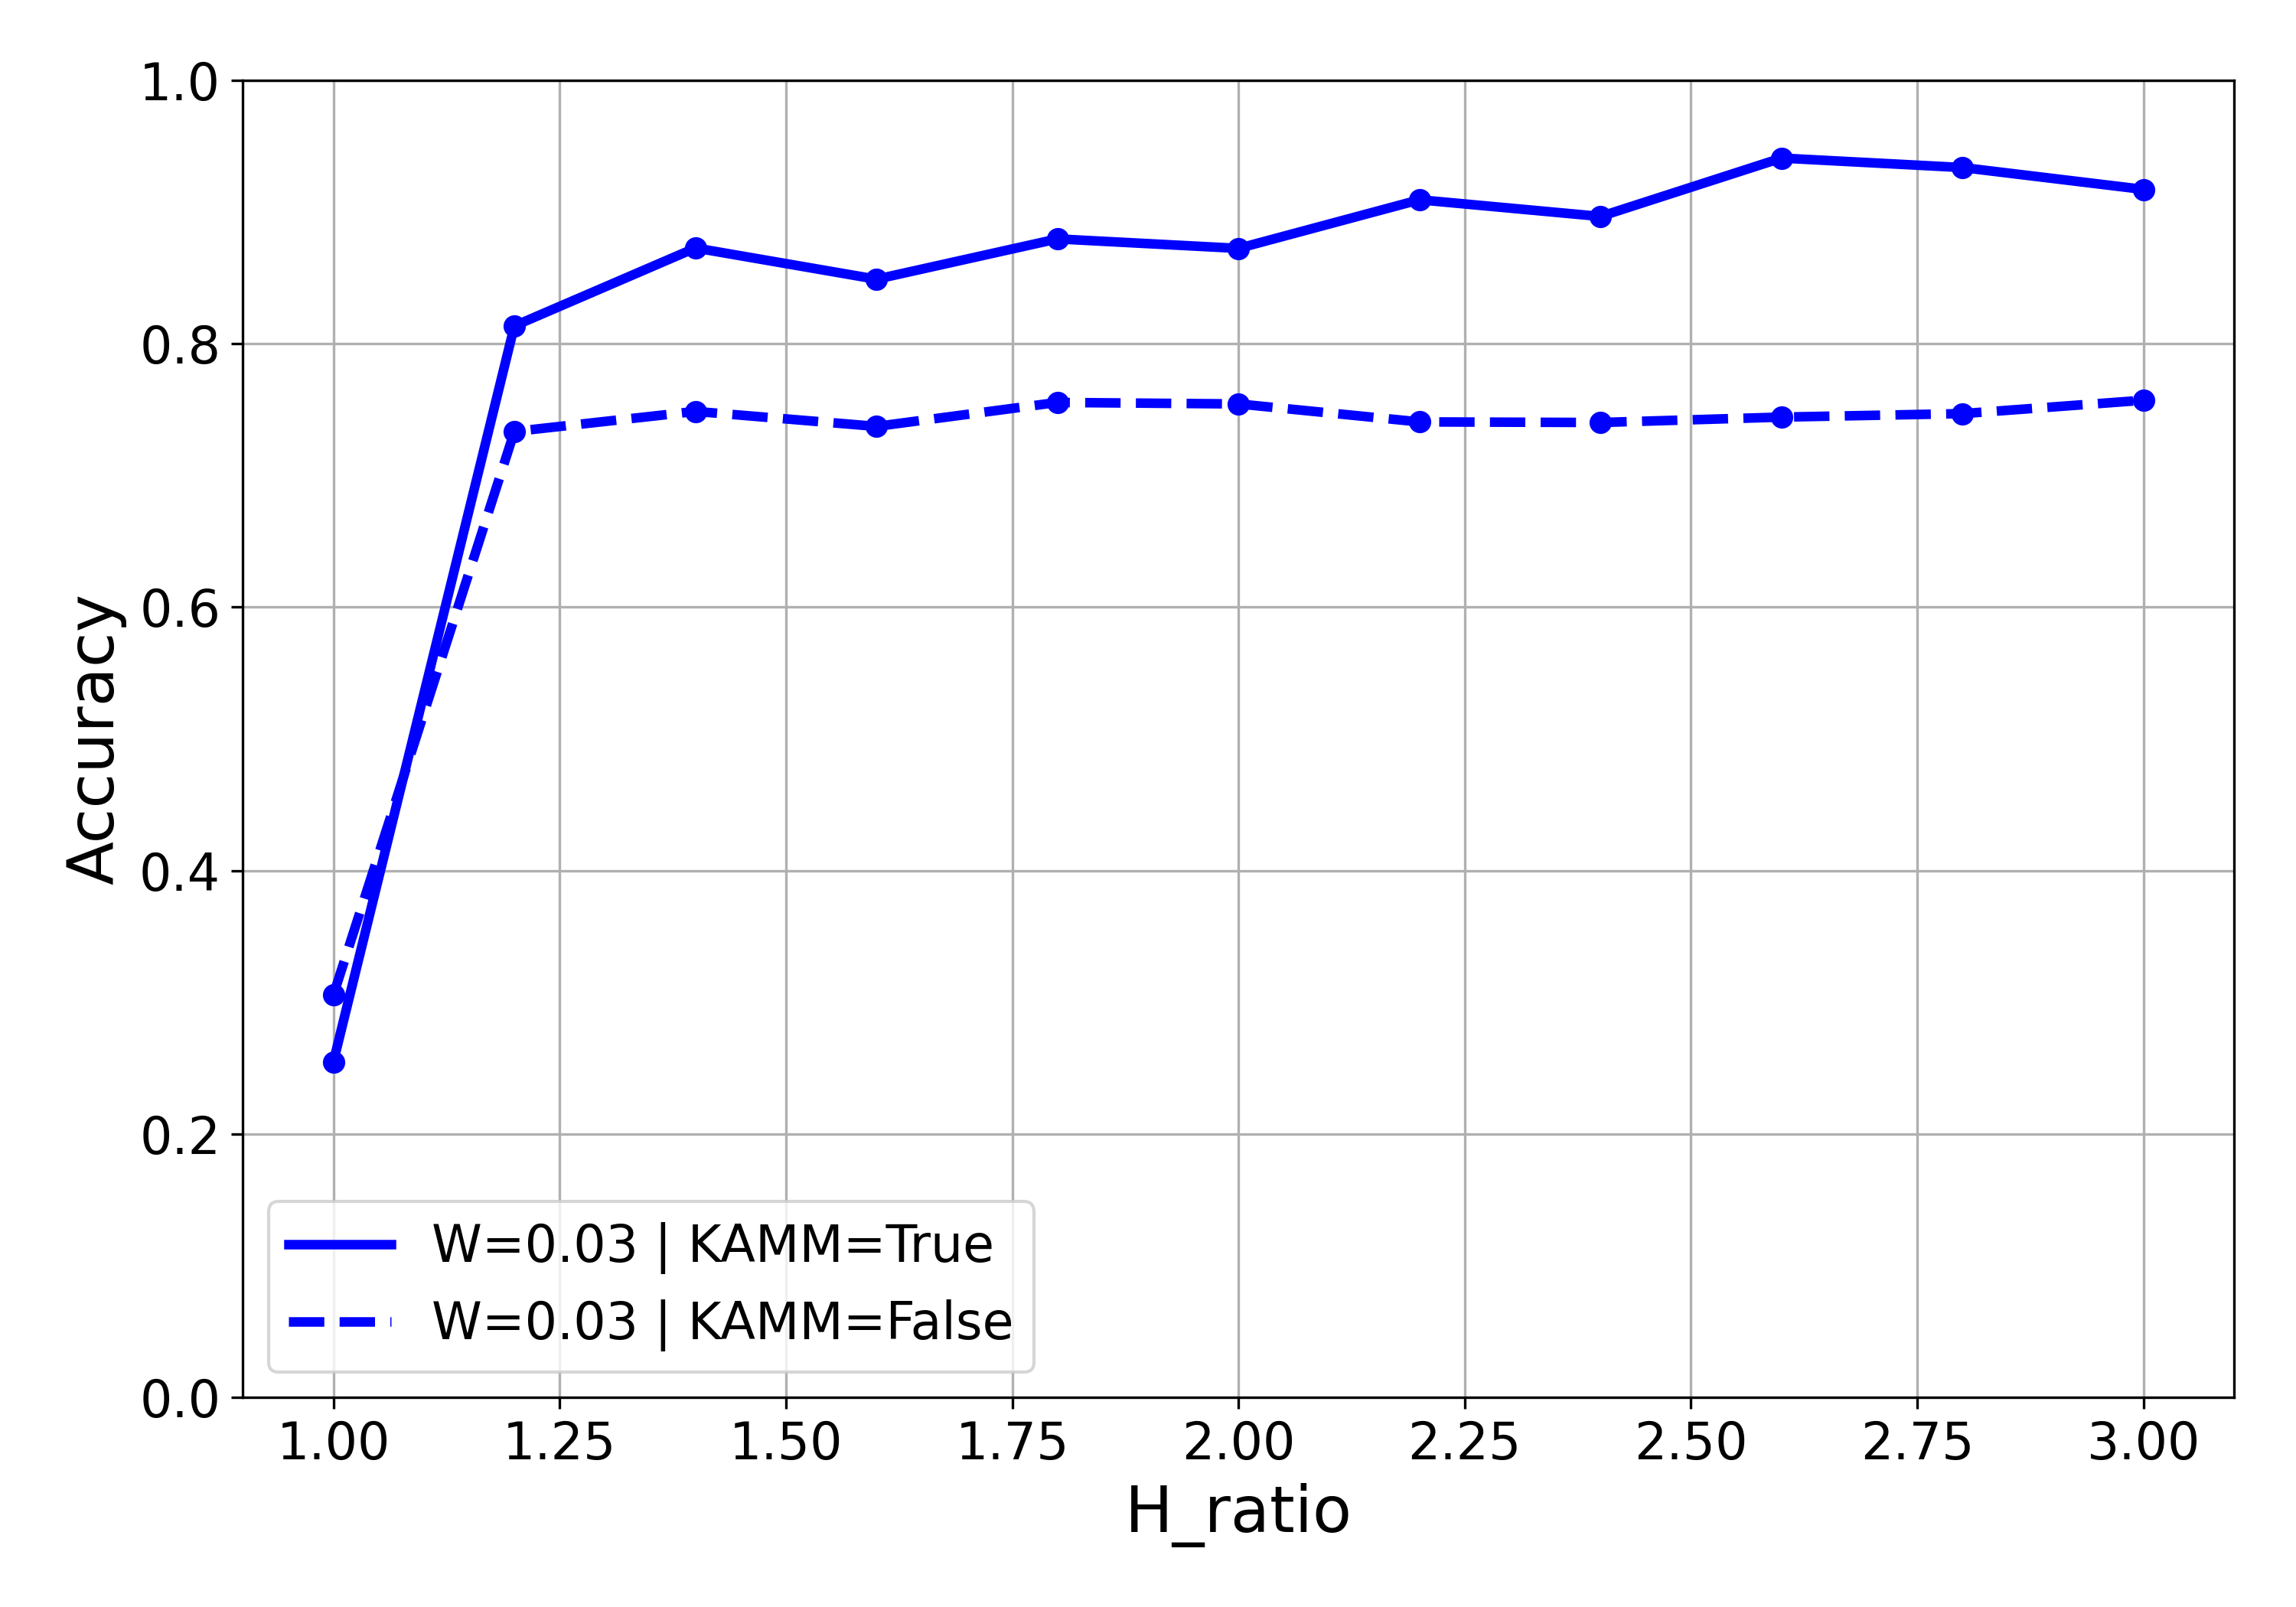
\includegraphics[width=\linewidth]{pictures/Accuracy_MultiSpecimen_AgglomerativeClustering_Graded.png}
    }
\end{minipage}
\hfill
\begin{minipage}{0.45\textwidth}
    \subfloat[DBSCAN]{
        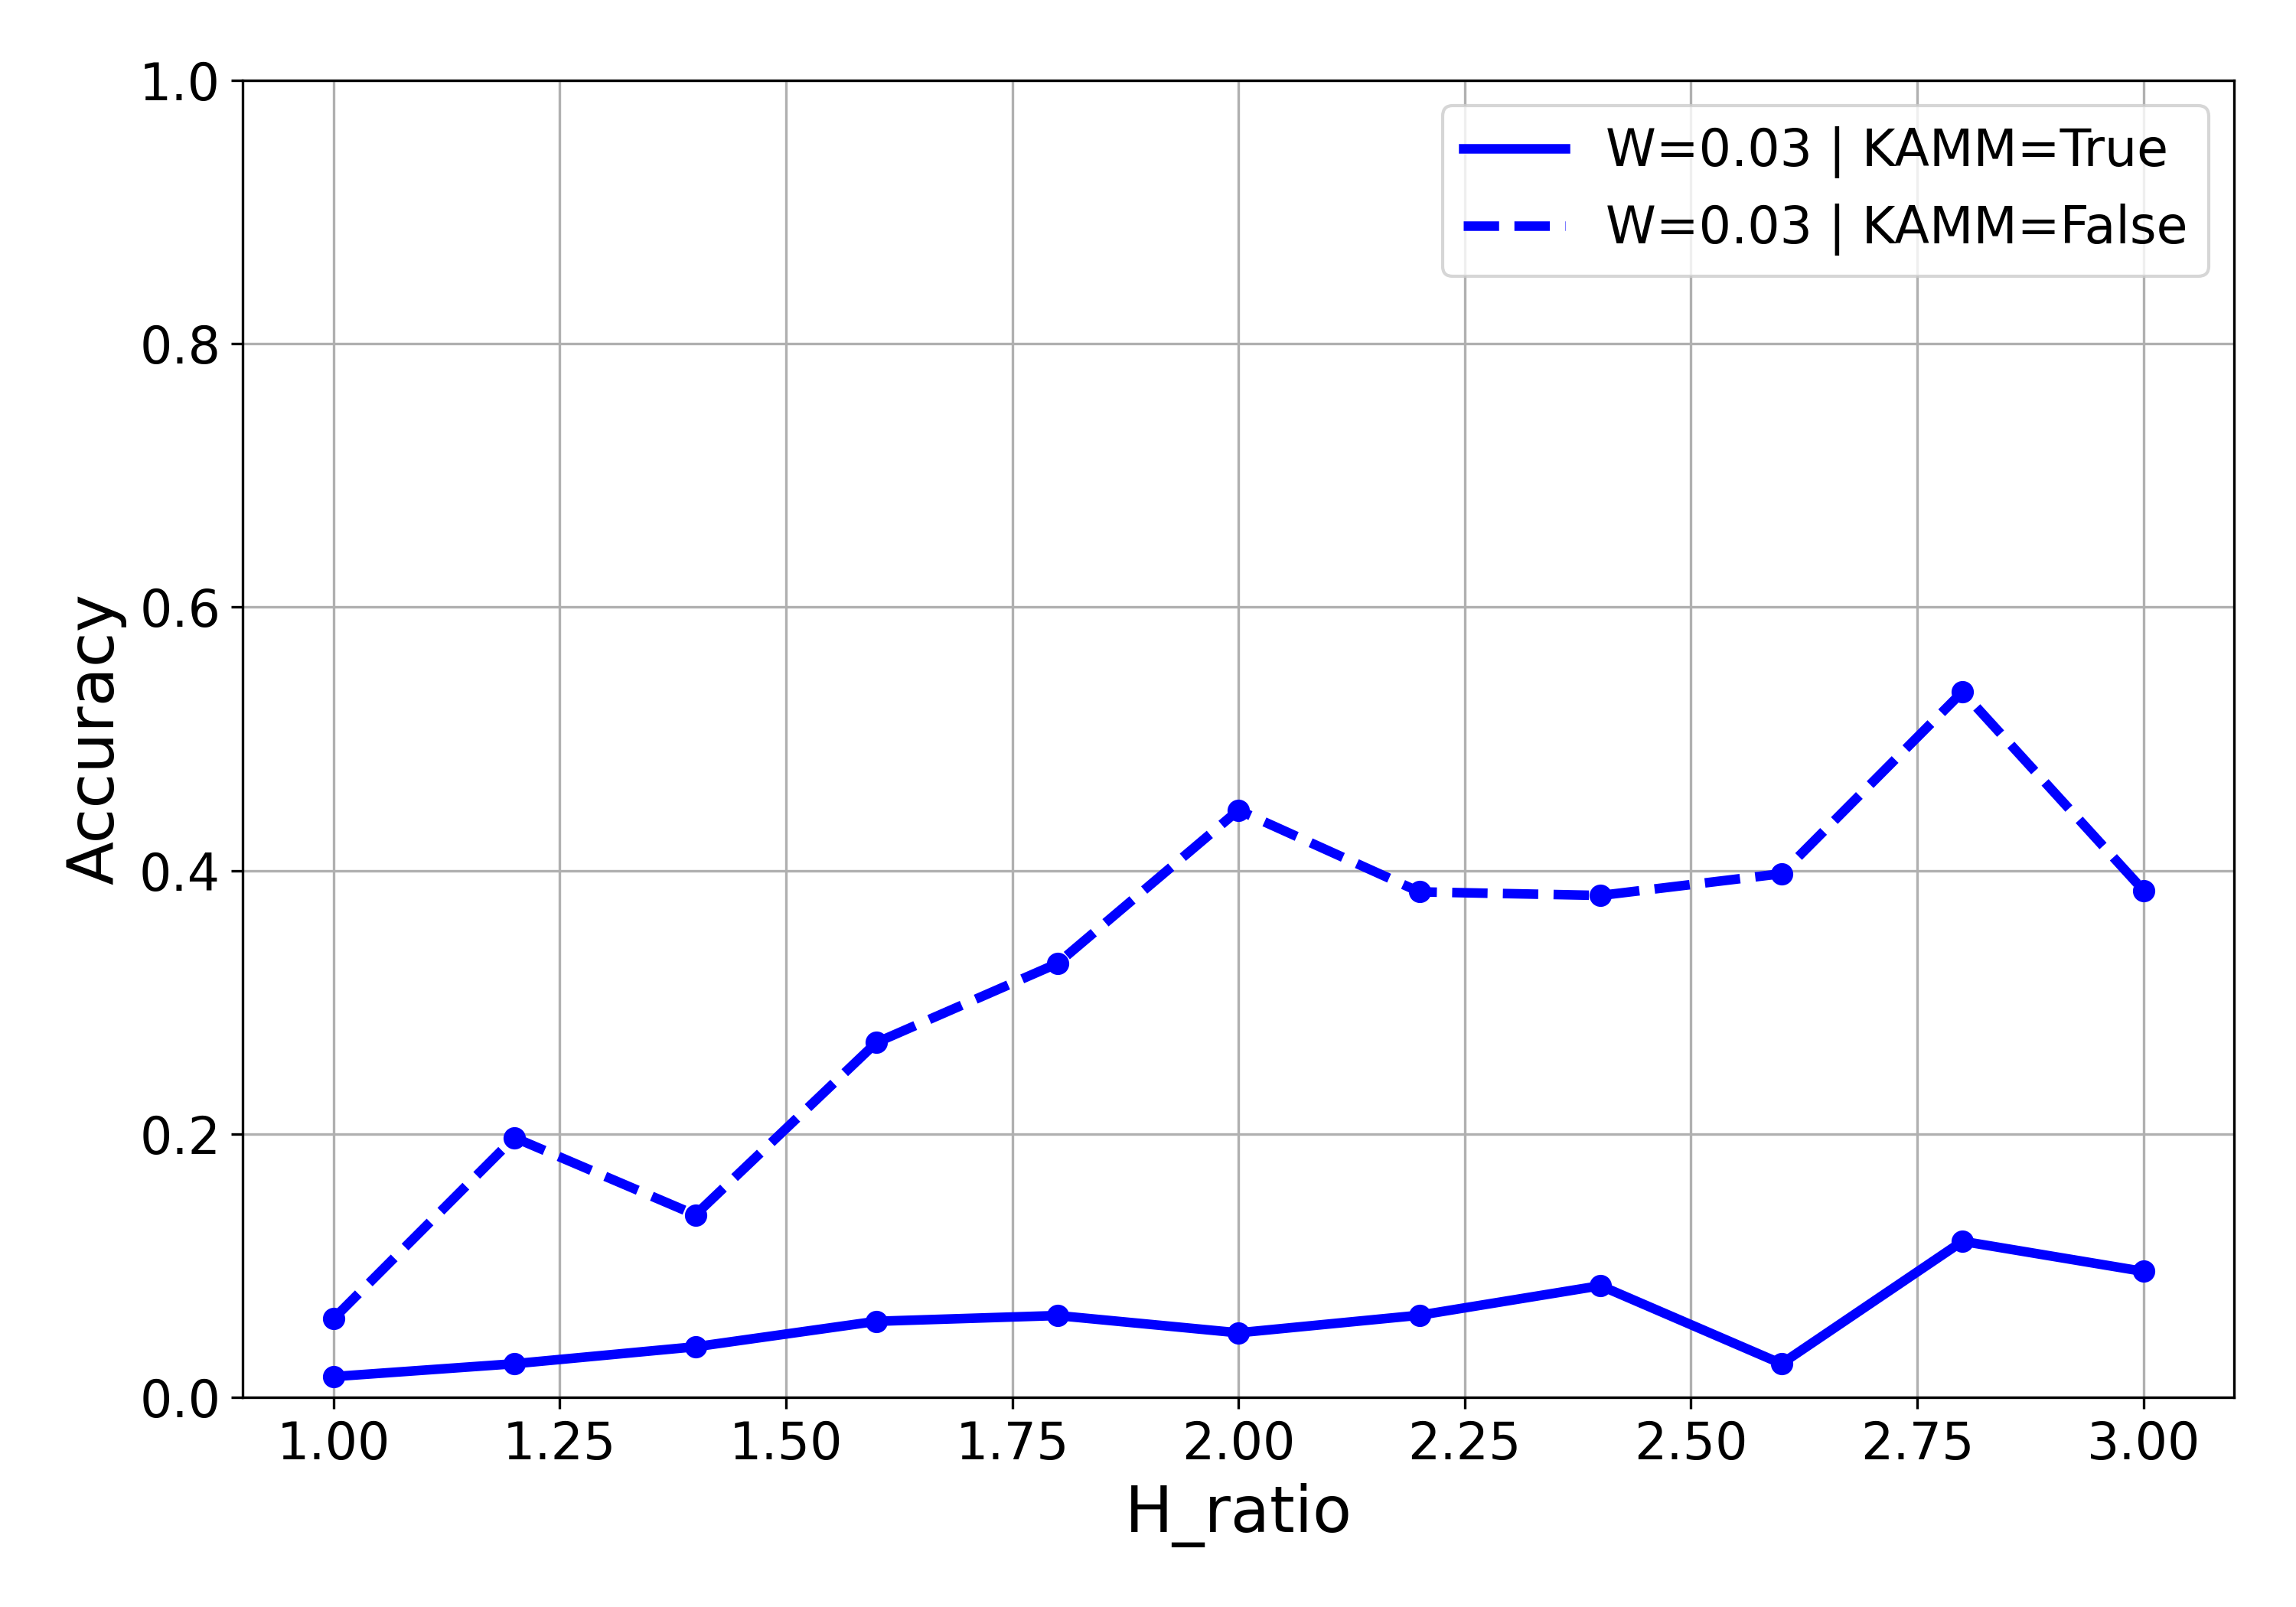
\includegraphics[width=\linewidth]{pictures/Accuracy_MultiSpecimen_DBSCAN_Graded.png}
    }
\end{minipage}

\vspace{0.3cm}

% --- Row 2 ---
\begin{minipage}{0.45\textwidth}
    \subfloat[GMM]{
        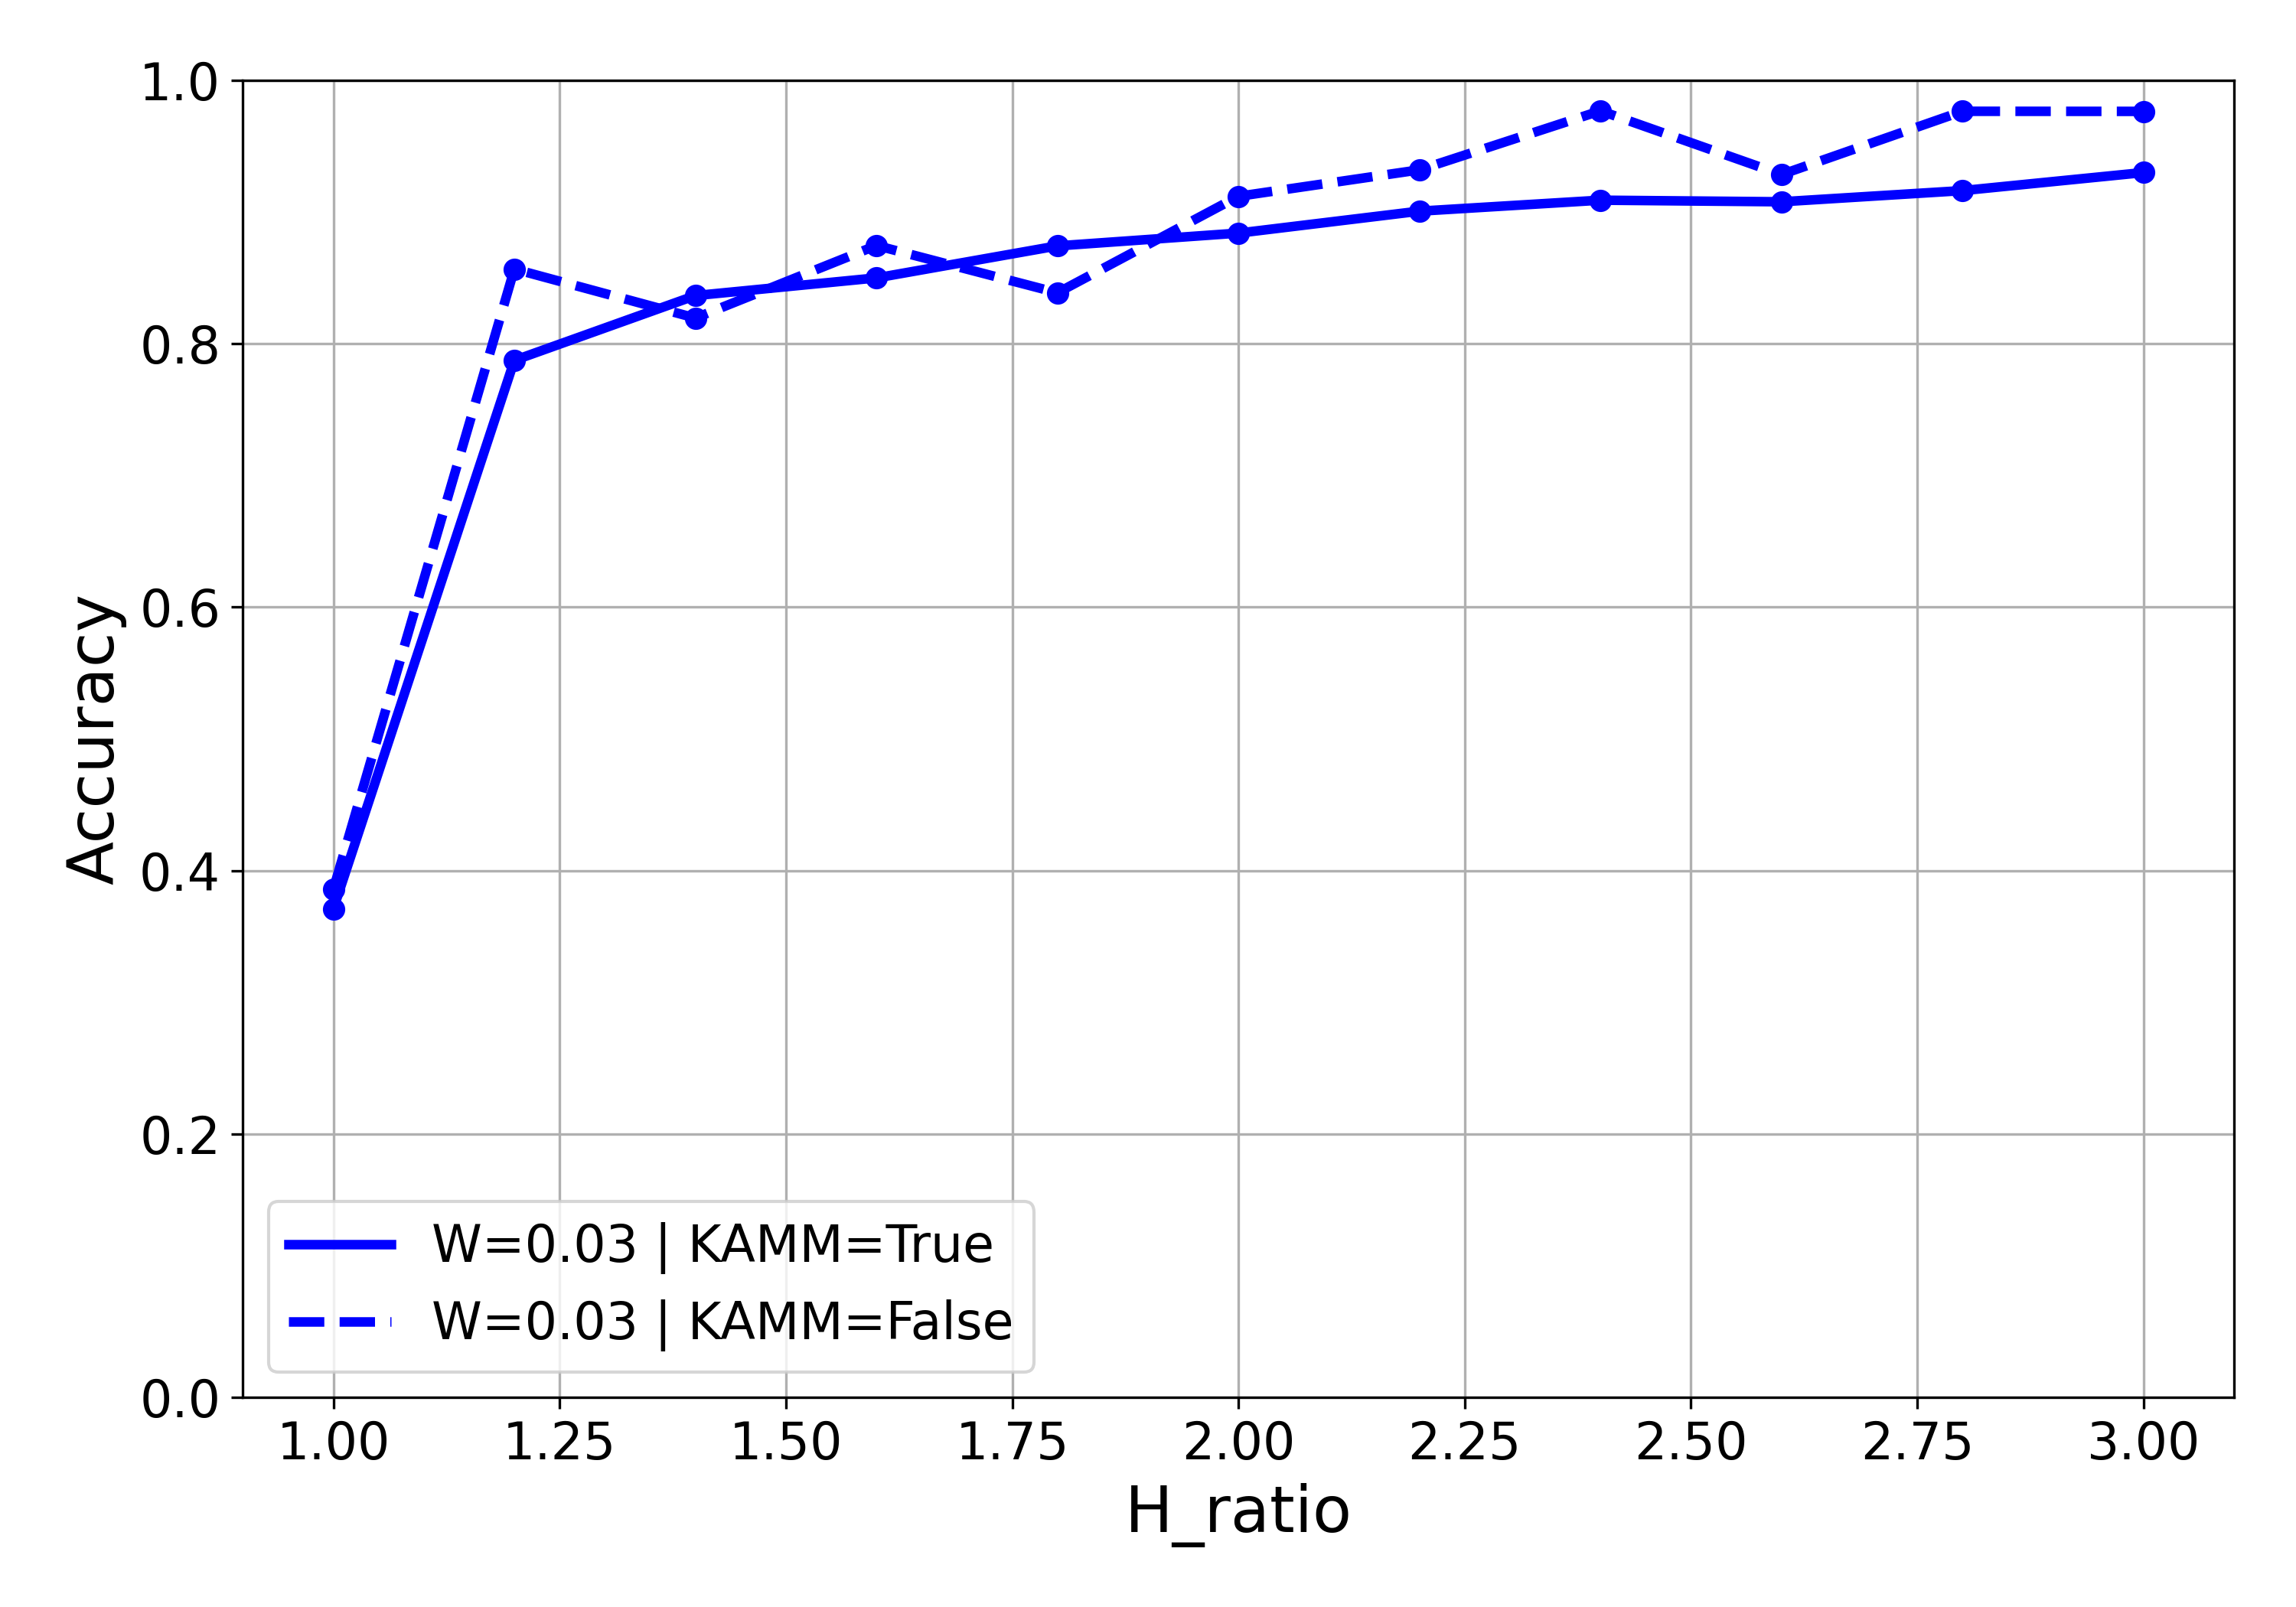
\includegraphics[width=\linewidth]{pictures/Accuracy_MultiSpecimen_GMM_Graded.png}
    }
\end{minipage}
\hfill
\begin{minipage}{0.45\textwidth}
    \subfloat[KMeans]{
        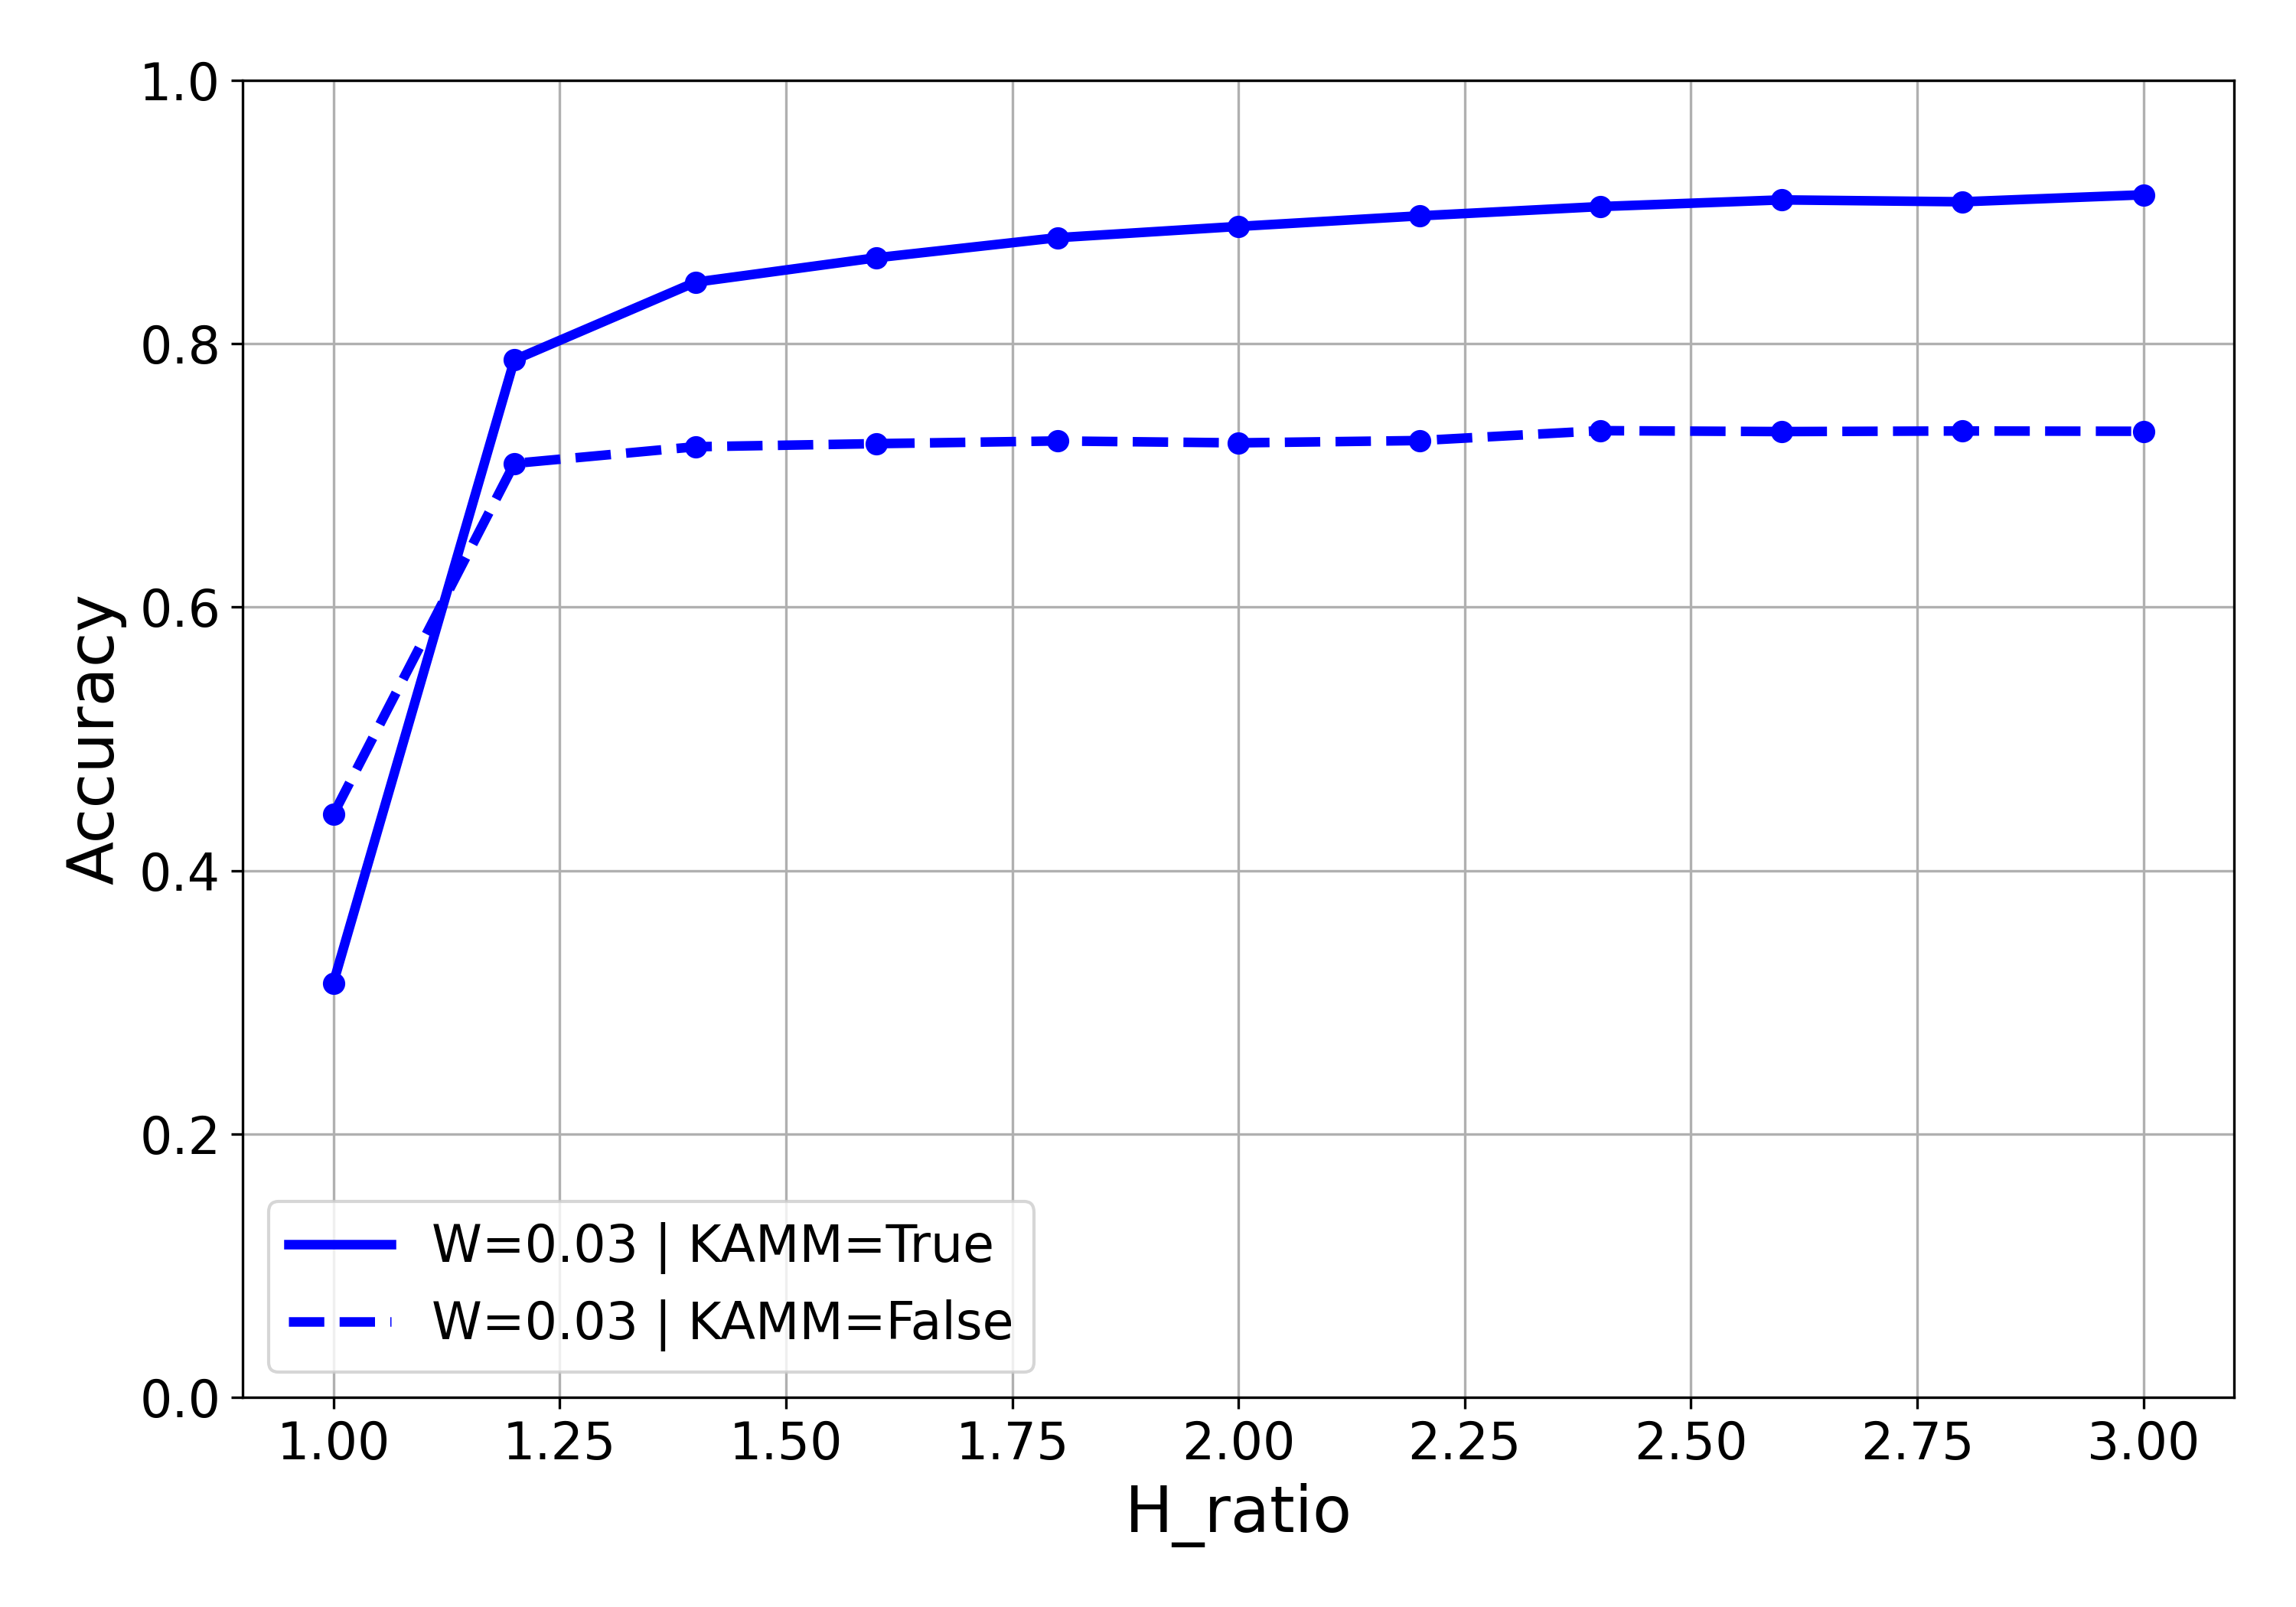
\includegraphics[width=\linewidth]{pictures/Accuracy_MultiSpecimen_KMeans_Graded.png}
    }
\end{minipage}

\vspace{0.4cm}

\caption{
Clustering accuracy at pixel level vs.\ hardness contrast ($H_\mathrm{ratio}$) for graded interphase ($W=0.03$) in the case of rectangular composite. Solid lines: clustering with KAMM; dashed lines: $(E,H)$-only baseline.
}
\label{fig:Clustering_GradedInterphase}
\end{figure}

\subsection{Matrix--fiber and matrix--particle specimens}
\label{sec:results_matrix-particles}

Figure~\ref{fig:Clustering_MatrixParticles} compares the clustering accuracy obtained for three configurations: a matrix--fiber composite with a sharp matrix--fiber interface ($W=0$), a matrix--fiber composite with a graded annular interphase ($W=0.05$), and a matrix--particle composite with diffuse randomly distributed inclusions. For each algorithm, the curves compare the performance with and without the KAMM descriptor as a function of the hardness contrast $H_\mathrm{ratio}$.

\begin{figure}[htbp]
\centering

% --- Row 1 ---
\begin{minipage}{0.45\textwidth}
    \subfloat[Agglomerative Clustering]{
        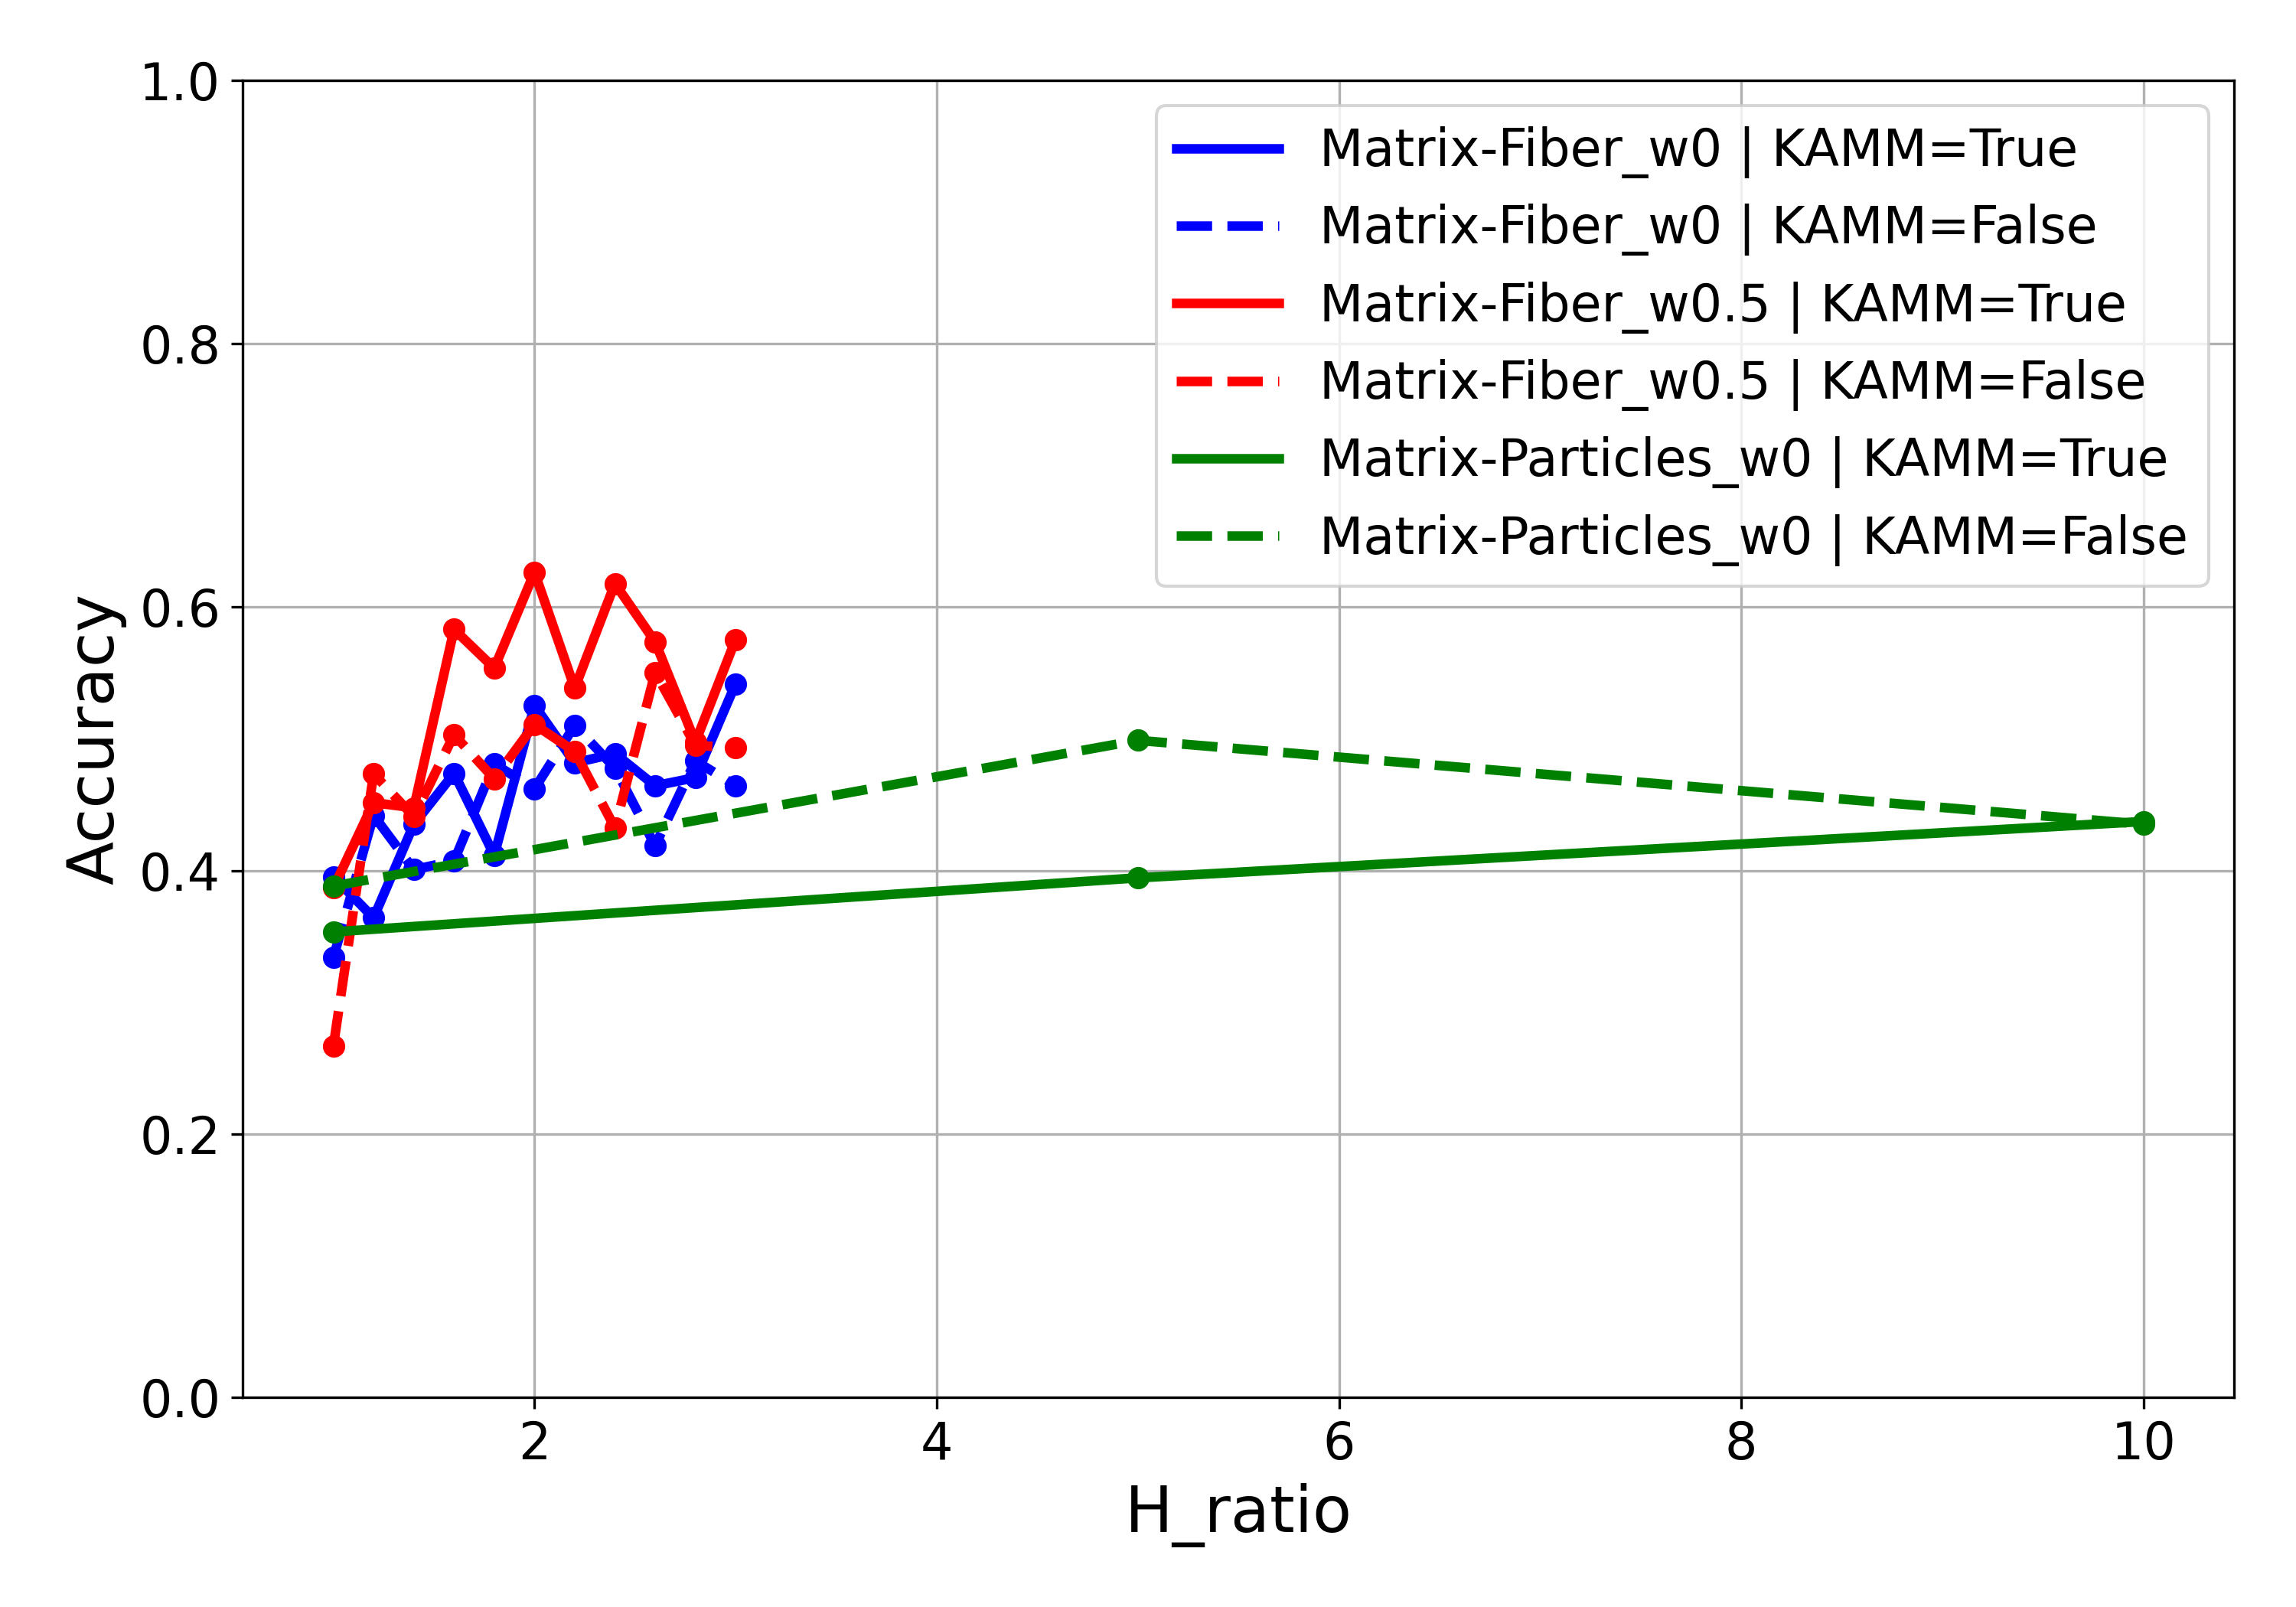
\includegraphics[width=\linewidth]{pictures/Accuracy_MatrixParticles_AgglomerativeClustering.png}
    }
\end{minipage}
\hfill
\begin{minipage}{0.45\textwidth}
    \subfloat[DBSCAN]{
        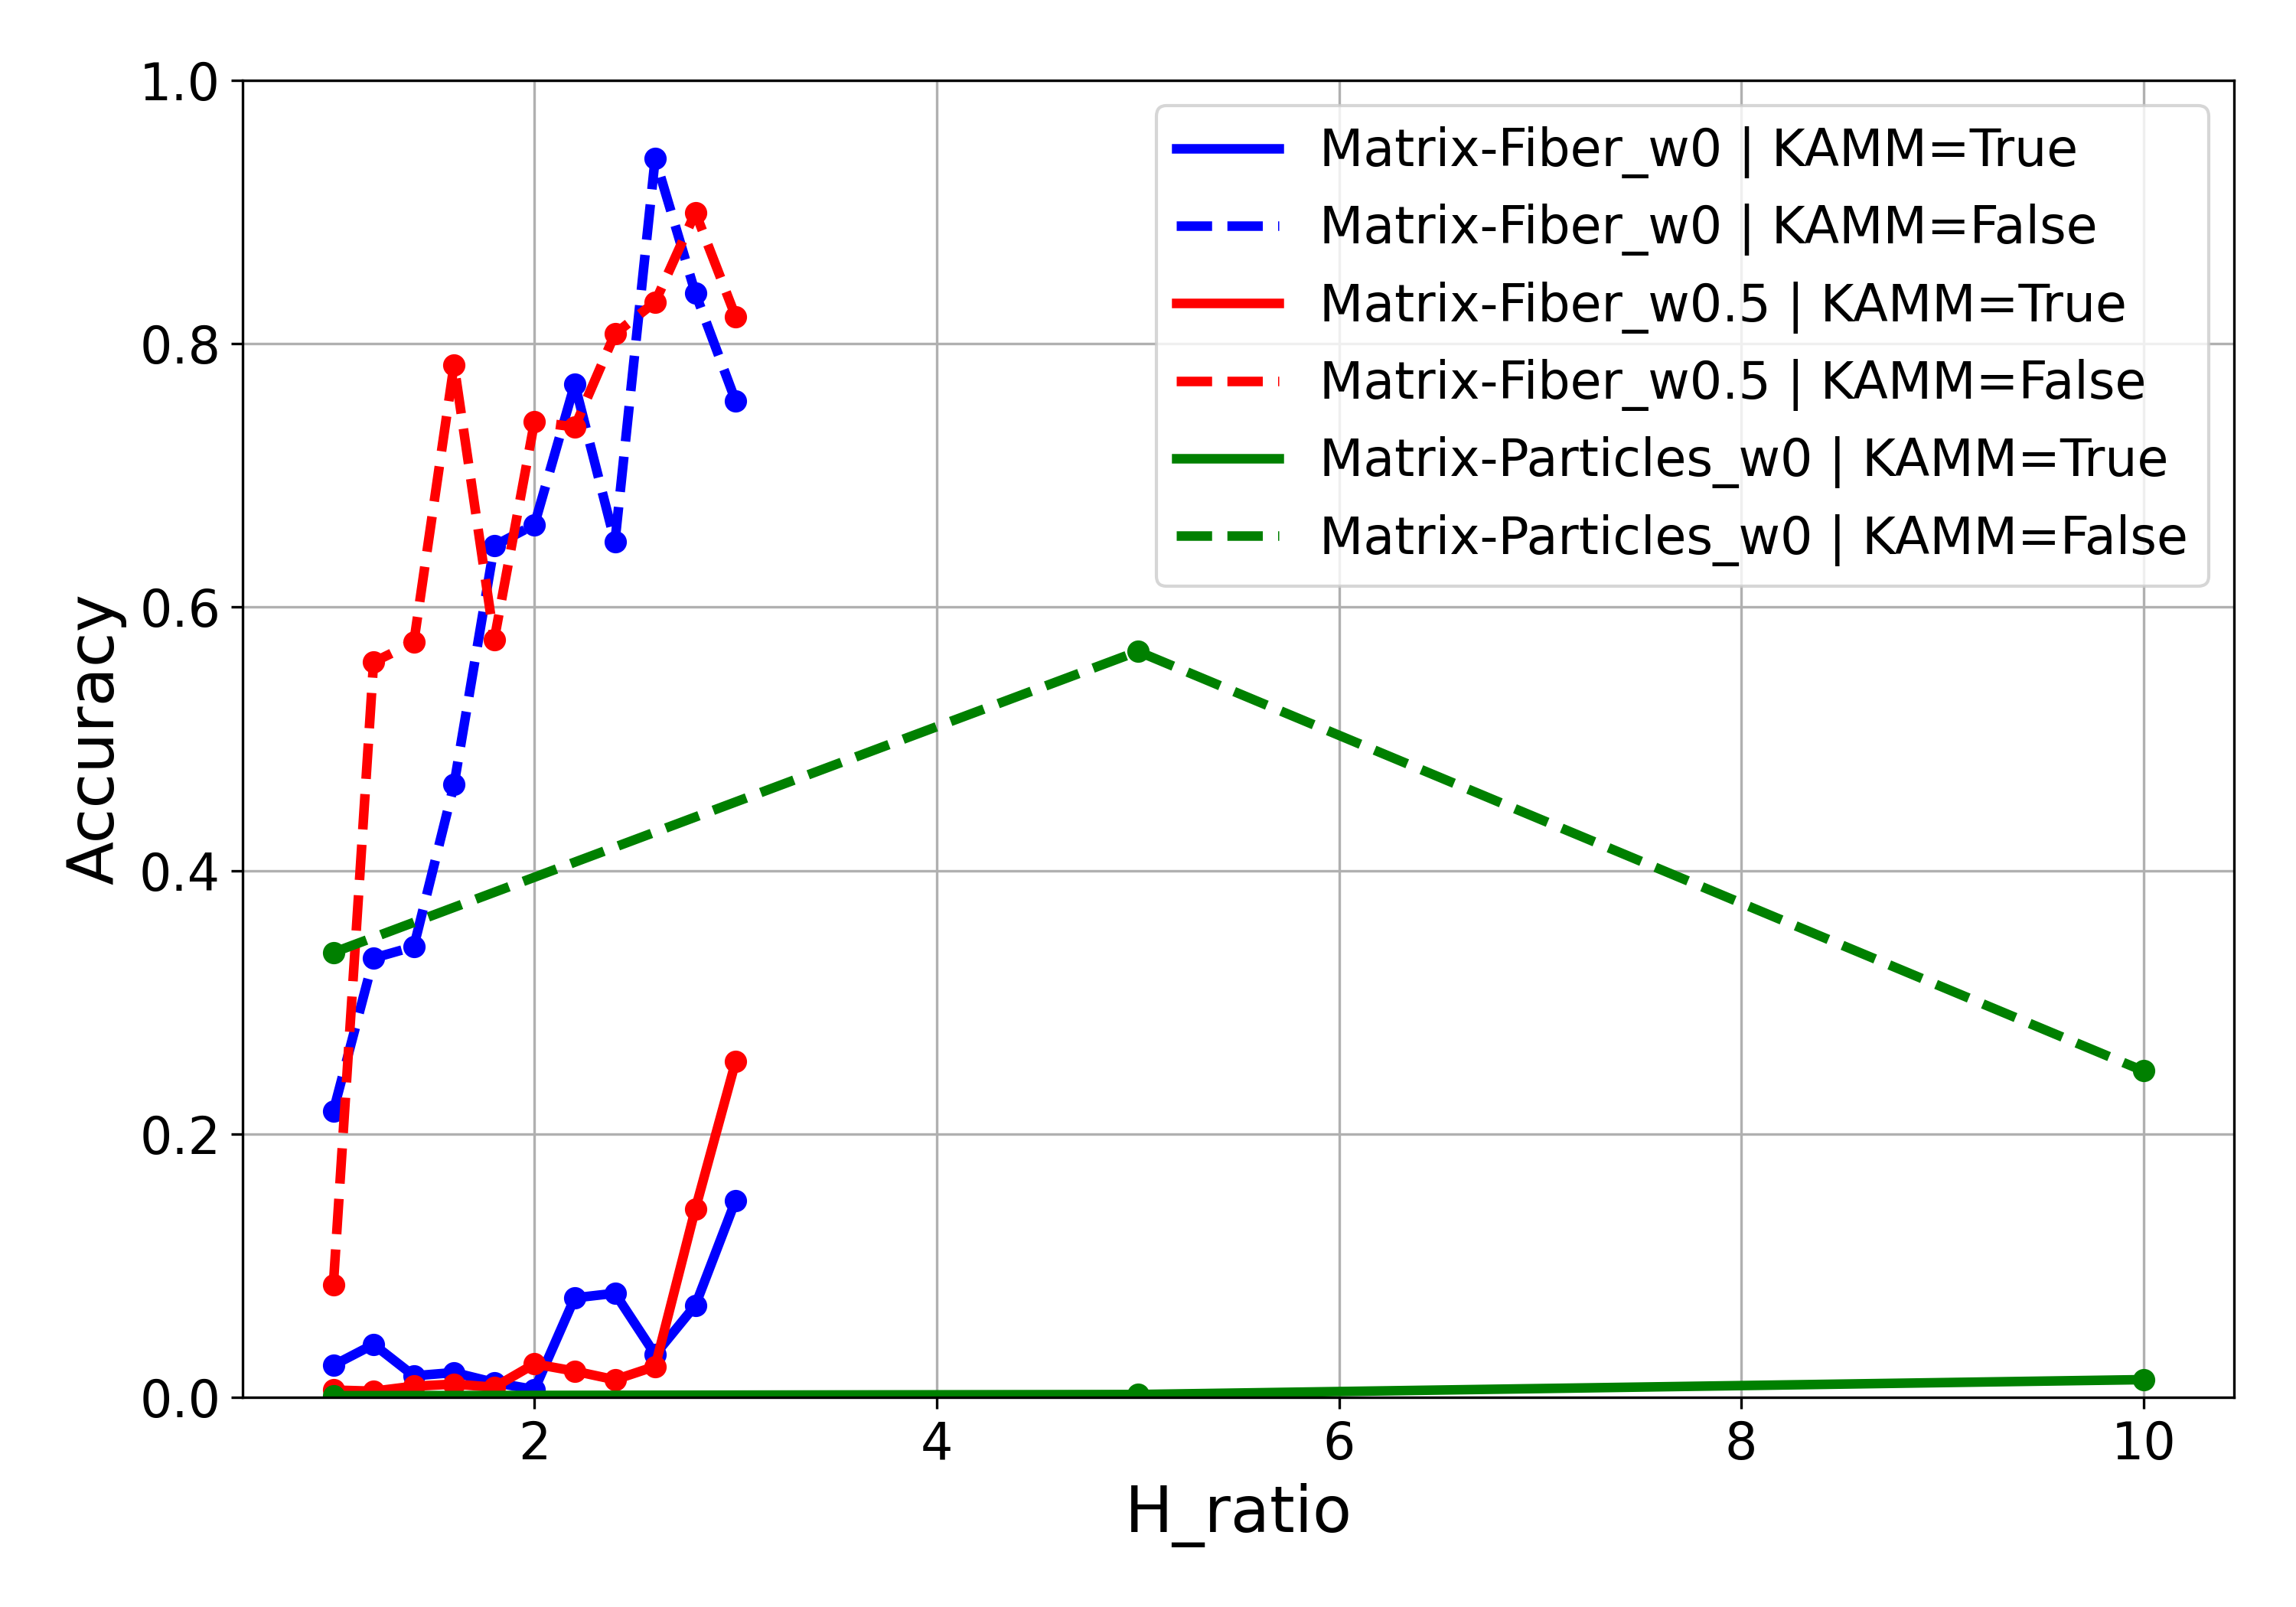
\includegraphics[width=\linewidth]{pictures/Accuracy_MatrixParticles_DBSCAN.png}
    }
\end{minipage}

\vspace{0.3cm}

% --- Row 2 ---
\begin{minipage}{0.45\textwidth}
    \subfloat[GMM]{
        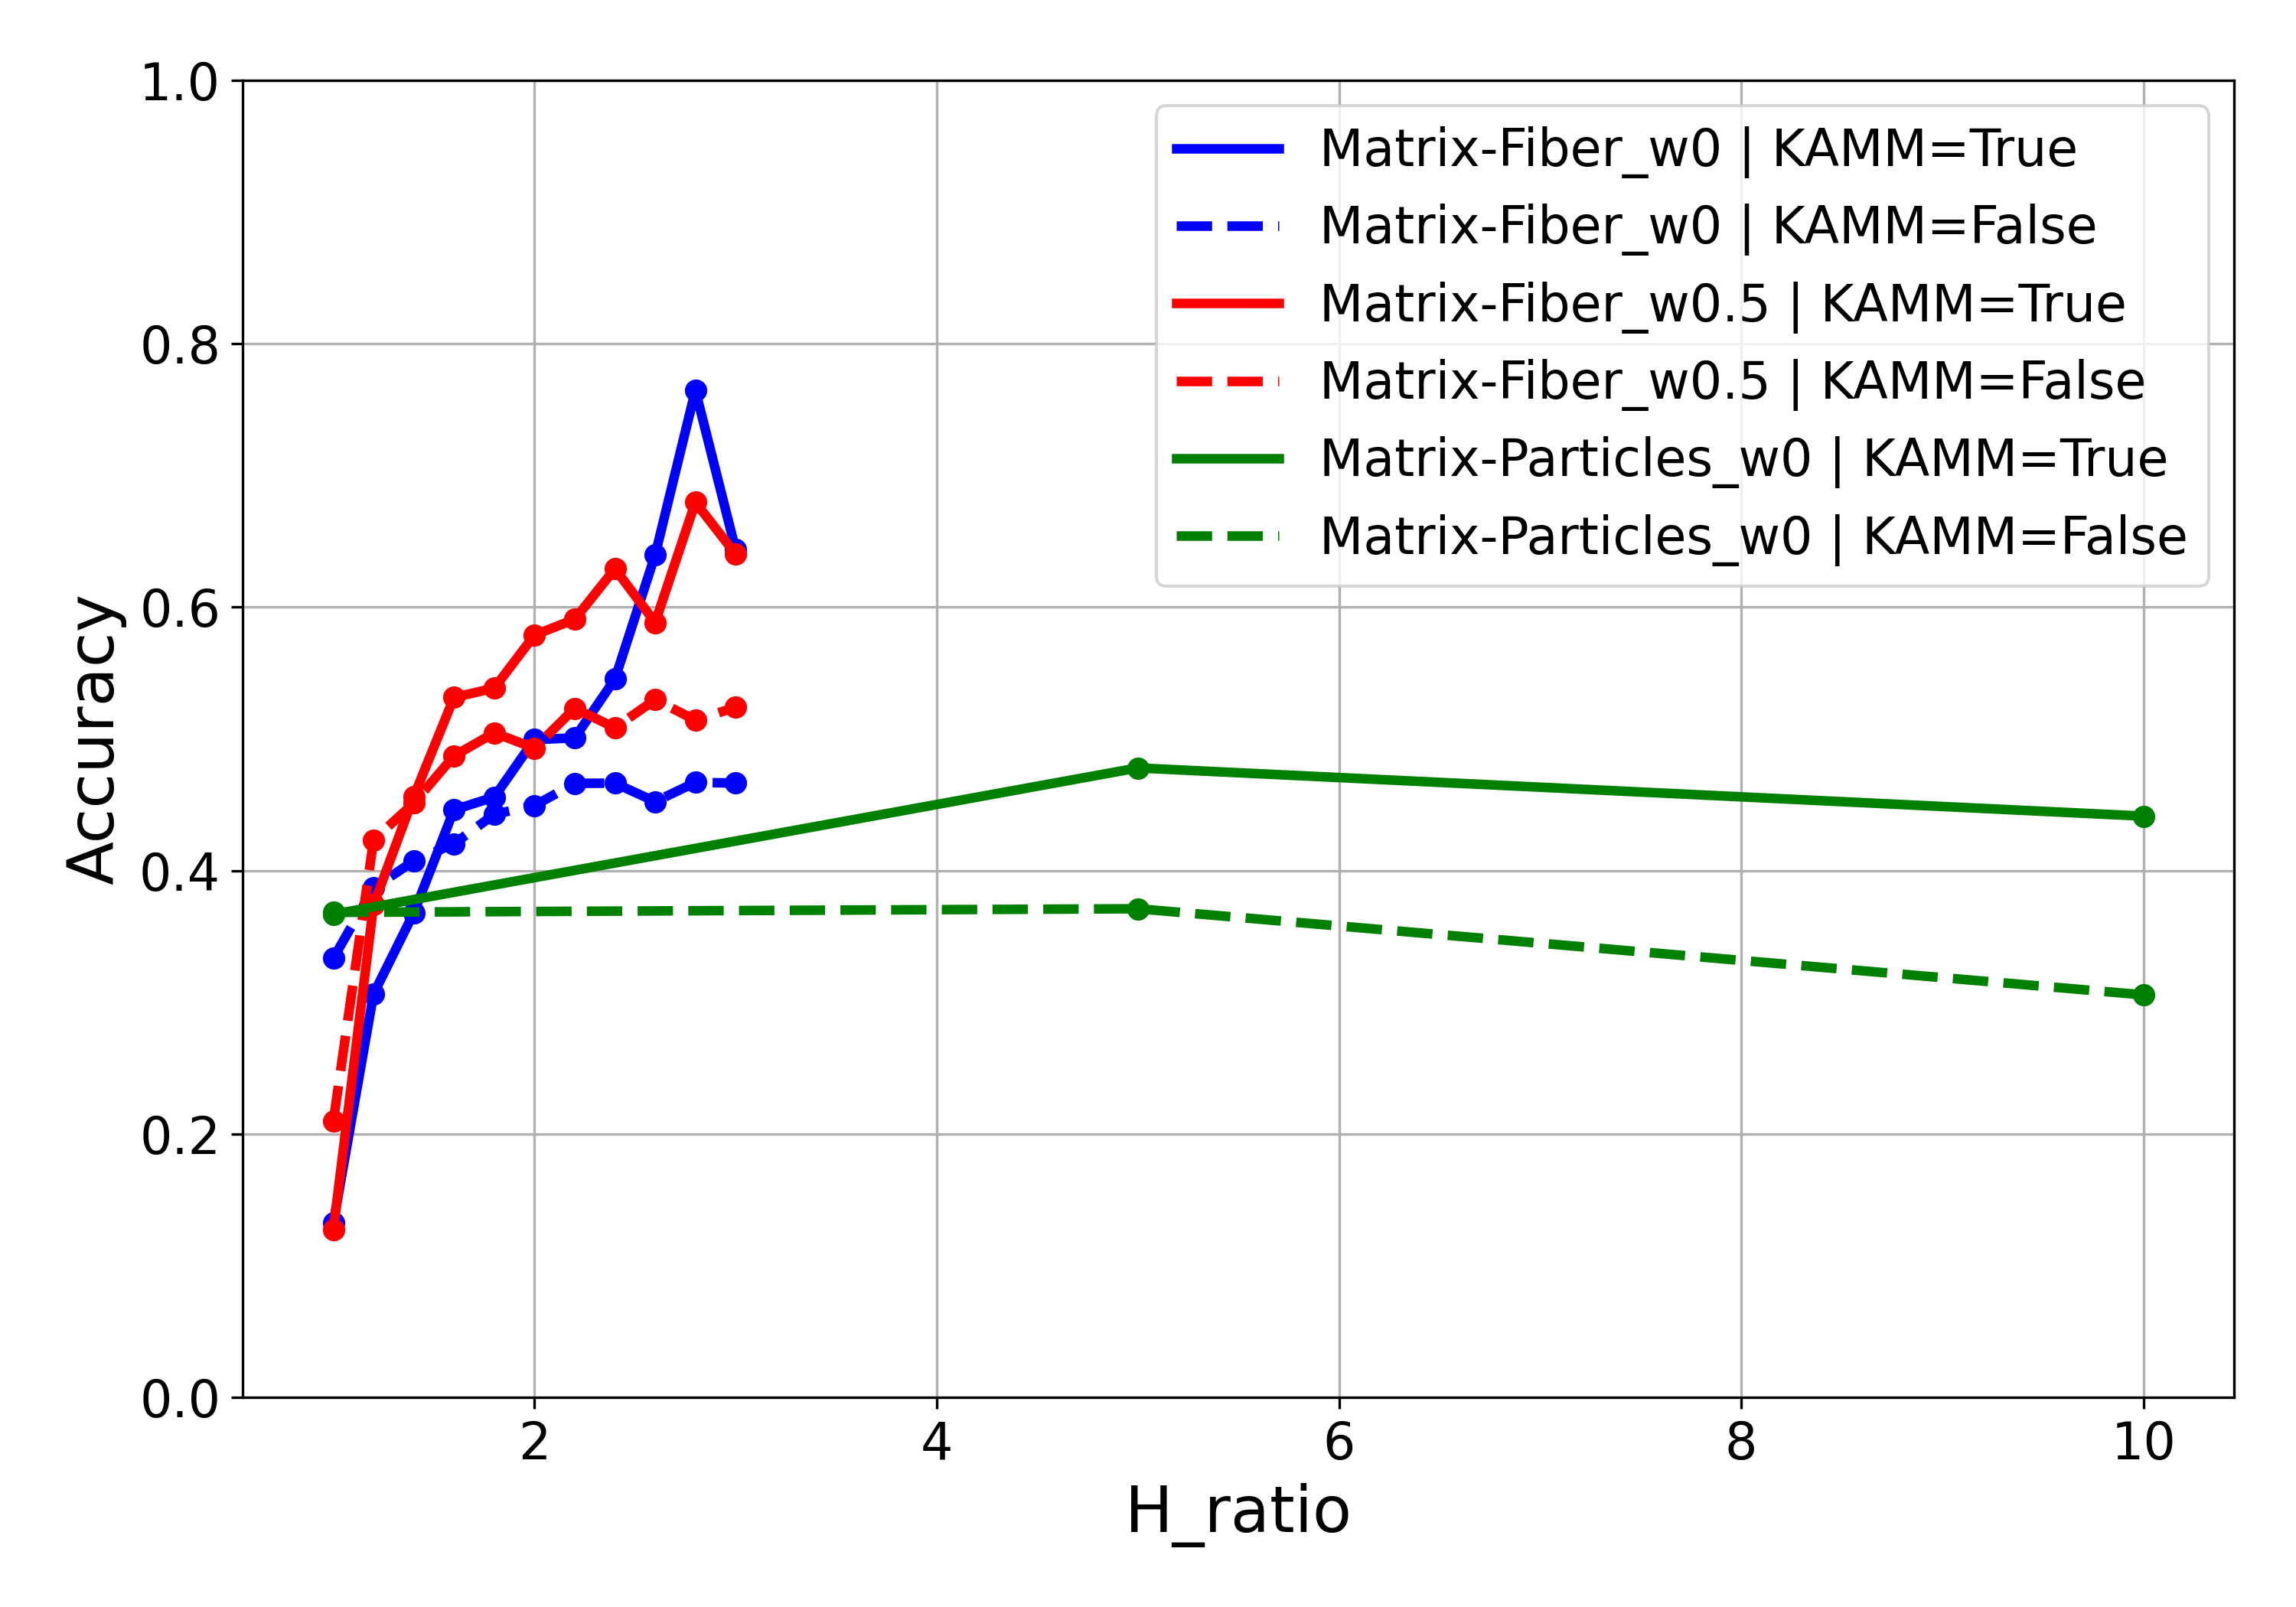
\includegraphics[width=\linewidth]{pictures/Accuracy_MatrixParticles_GMM.png}
    }
\end{minipage}
\hfill
\begin{minipage}{0.45\textwidth}
    \subfloat[KMeans]{
        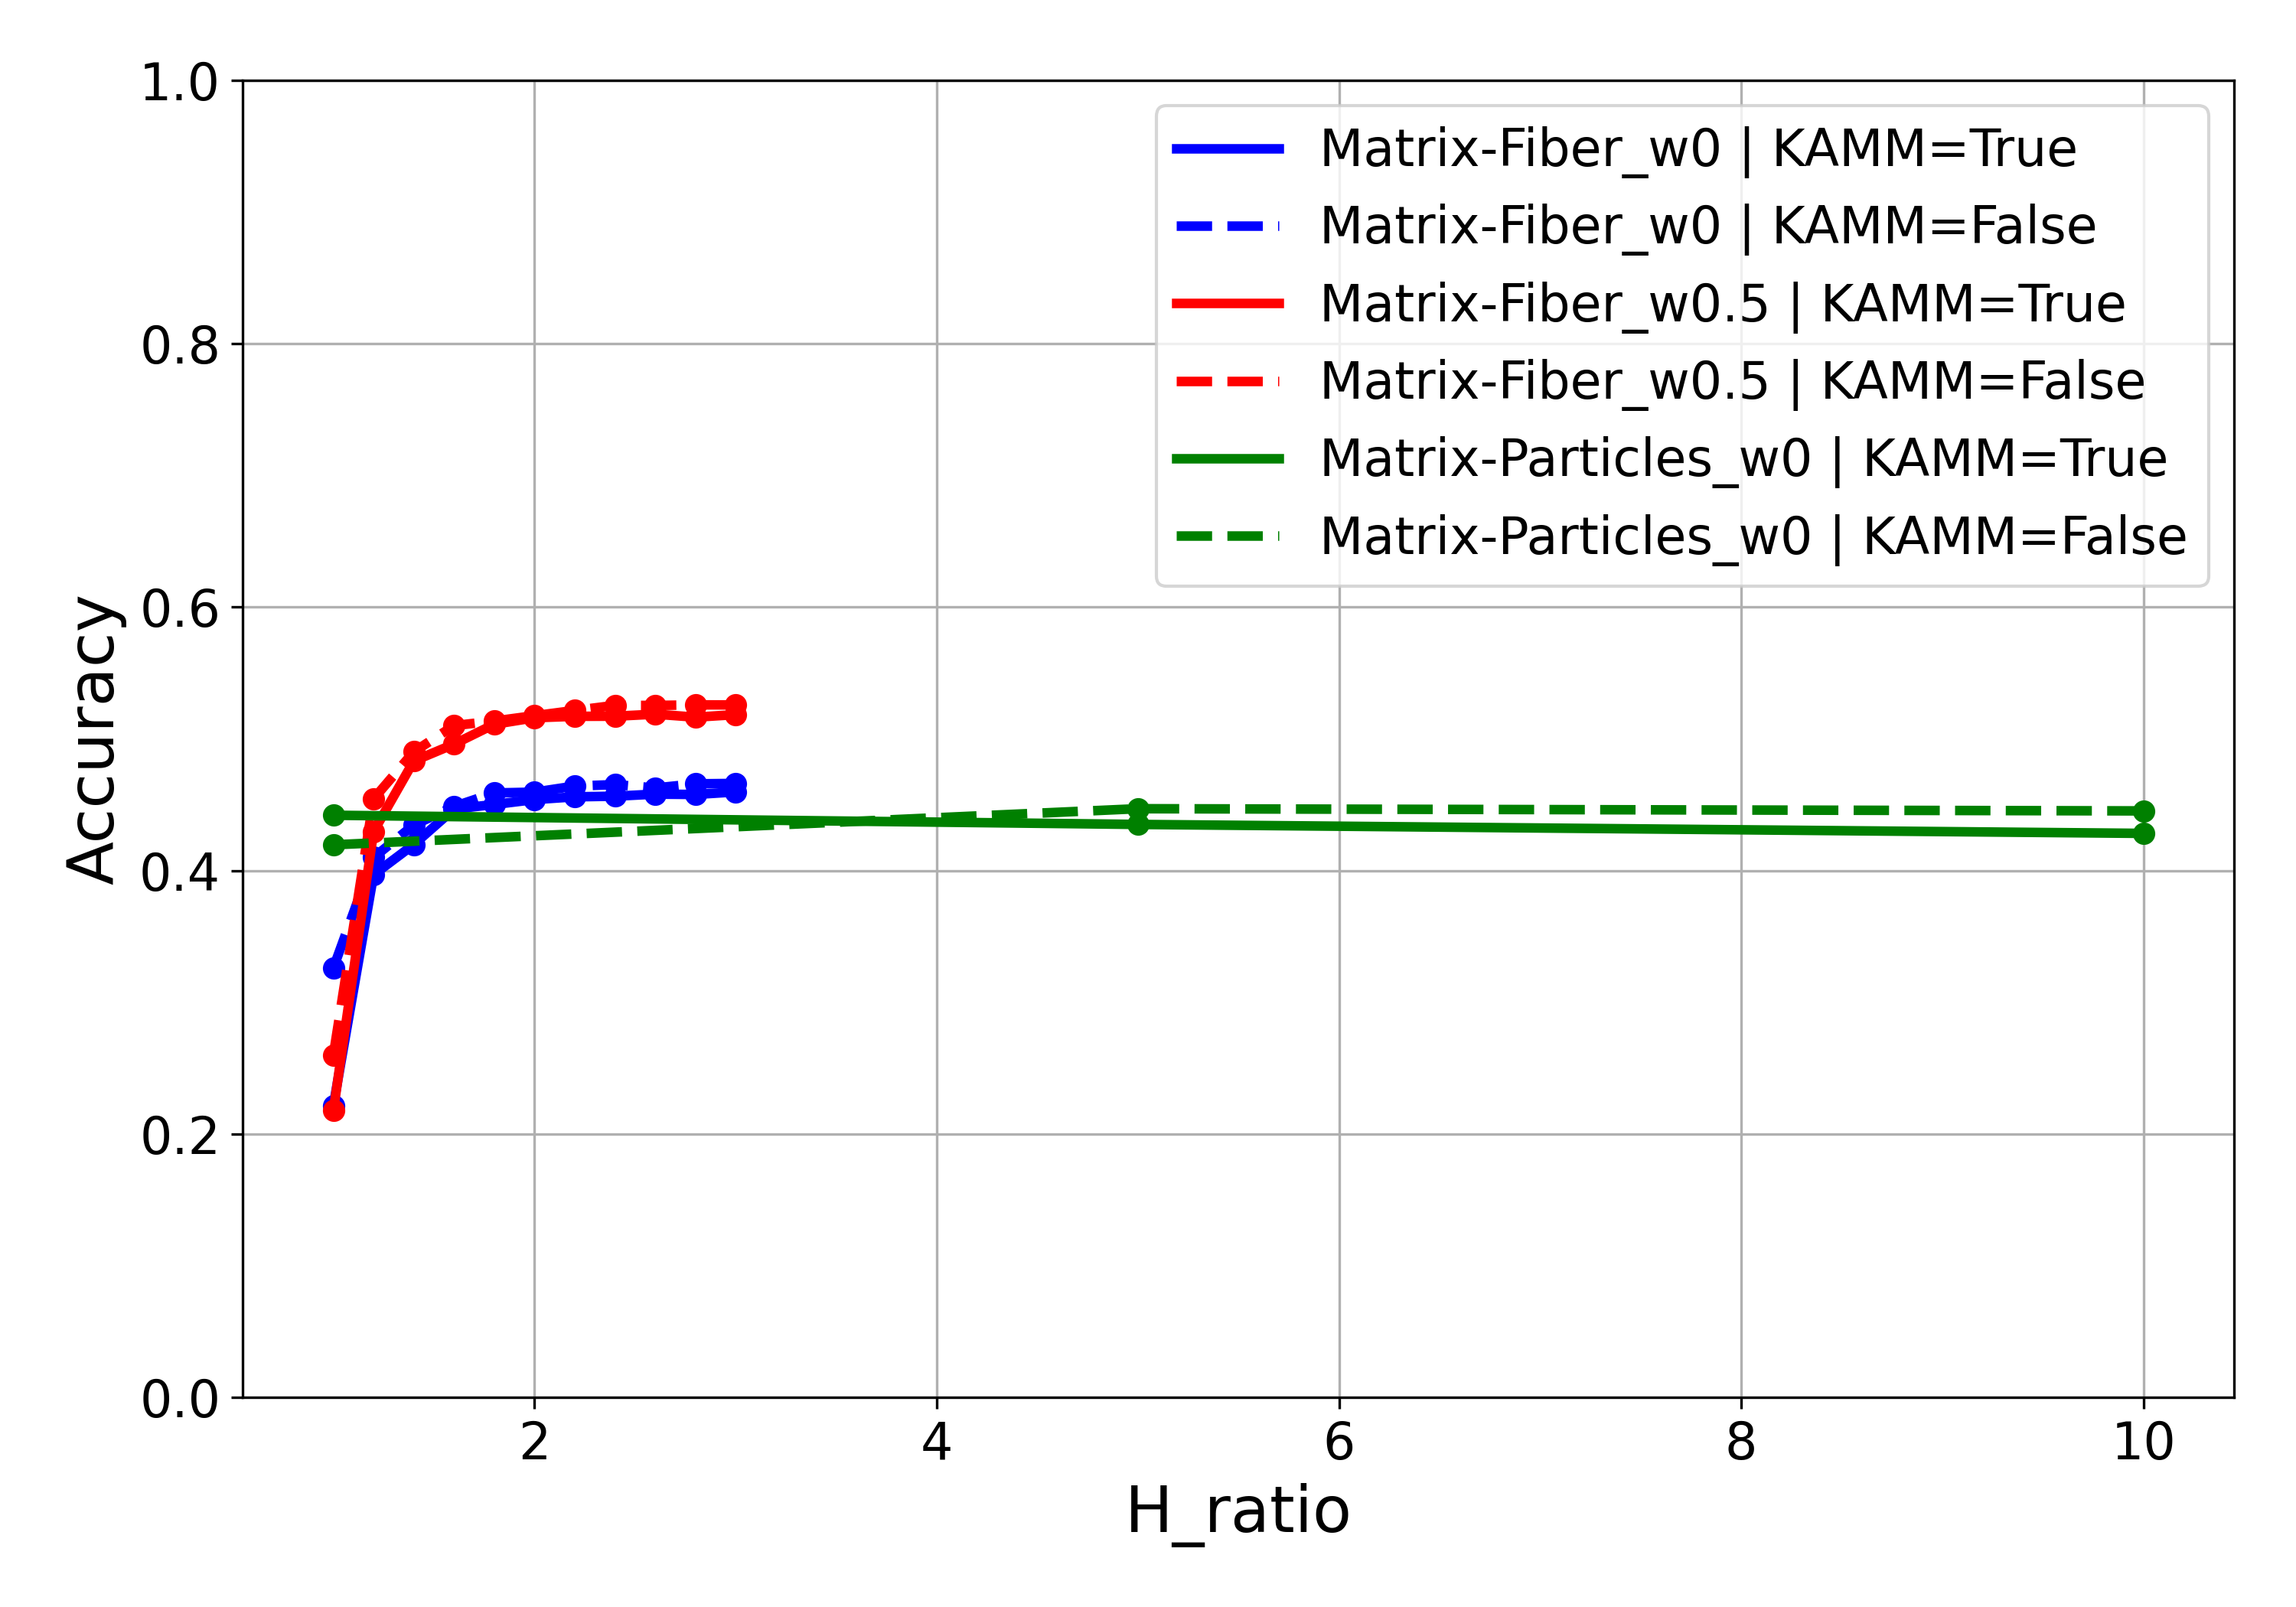
\includegraphics[width=\linewidth]{pictures/Accuracy_MatrixParticles_KMeans.png}
    }
\end{minipage}

\vspace{0.4cm}

\caption{ Pixel-level clustering accuracy as a function of hardness contrast ($H_\mathrm{ratio}$) for a matrix--fiber composite with a sharp interface, a matrix--fiber composite with a graded annular interphase ($W=0.05$), and a matrix--particle composite with diffuse random inclusions. Solid lines denote clustering with KAMM; dashed lines denote the $(E,H)$-only baseline. }
\label{fig:Clustering_MatrixParticles}
\end{figure}

For Agglomerative Clustering, the influence of KAMM strongly depends on the microstructural configuration. For the matrix--fiber composite with a graded annular interphase ($W=0.05$), including KAMM clearly improves clustering accuracy across most hardness ratios. In contrast, little to no difference is observed for the matrix--fiber composite with a sharp interface and the matrix--particle composite with diffuse inclusions, indicating that the hierarchical scheme benefits from KAMM primarily when the underlying gradients are spatially diffuse. For DBSCAN, the trends differ markedly. Across all three specimen types, accuracy is consistently higher when KAMM is not included. The mismatch-based descriptor appears to deteriorate density-based segmentation, likely because it amplifies local variability that DBSCAN interprets as noise, thereby fragmenting clusters and lowering accuracy. The behavior of GMM is opposite: for all specimen types, introducing KAMM increases accuracy, particularly at intermediate hardness ratios. These results indicate that Gaussian mixture models effectively exploit the additional variability encoded in the KAMM descriptor, leading to a more informative probabilistic partition of the data. Finally, for KMeans, the curves with and without KAMM nearly overlap for all three specimens. This suggests that centroid-based clustering is largely insensitive to KAMM, converging to similar partitions regardless of whether the mismatch descriptor is provided. Overall, the utility of KAMM is strongly algorithm-dependent. It provides clear benefits for GMM, selective improvement for Agglomerative Clustering, minimal influence for KMeans, and systematic degradation for DBSCAN.

\subsection{Real experimental datasets}
\label{sec:results_experimental}

To examine the behavior of the proposed clustering framework under realistic measurement conditions, the method was subsequently applied to an experimental nanoindentation dataset. Unlike the synthetic benchmarks, this dataset does not provide pixel-level ground-truth phase labels. The experimental analysis is therefore used to assess the practical behavior and physical interpretability of the method rather than as a supervised validation of clustering accuracy.

Particular attention is given to measurements located near apparent matrix--particle boundaries. Such measurements may exhibit intermediate mechanical responses resulting from a physical interphase, a mixed indentation response associated with the finite mechanically affected volume, measurement effects, or a combination of these factors. Because independent correlative information is not available at each indentation position, their origin cannot be established conclusively from the present dataset.

KAMM is therefore used to highlight regions of strong local mechanical heterogeneity rather than to classify these regions directly as measurement artefacts.
\subsubsection{Specimen description and first analysis}
\label{sec:nisic}

The specimen originates from the work of Mercier \textit{et al.}~\cite{mercier_microstructural_2019}. 
It consists of a thick nickel coating reinforced with micrometric silicon carbide (SiC) particles, electro-deposited onto a steel substrate. Microscopic observations (SEM, OM, EBSD) reveal a two-phase surface microstructure composed of approximately 80\% Ni and 20\% SiC. Nanoindentation mapping was performed using a Berkovich indenter on a \(25 \times 25\) grid, with a spacing \(d = 2\,\mu\text{m}\) in both the \(X\) and \(Y\) directions and a maximum indentation depth of \(50\,\text{nm}\). This experimental setup satisfies the recommended length-scale criteria~\cite{randall_nanoindentation_2009, mercier_tridimap_2018}:

\begin{itemize}
    \item \(h_{\max} \leq 0.1\,D\), where \(D\) is the characteristic microstructural length scale  
    (here \(D = 1.3\,\mu\text{m}\), the mean SiC particle diameter);
    \item \(h_{\max} > 3\,R_q\), where \(R_q\) is the average surface roughness;
    \item \(d > (10.5\text{-}21)\,h_{\max}\).
\end{itemize}

Reference mechanical properties indicate a substantial contrast between the Ni matrix and the SiC particles, with reported hardnesses of \(3.9 \pm 0.3\)\,GPa and \(11.7 \pm 3.0\)\,GPa, respectively. Previous deconvolution analyses of nanoindentation data have shown that both hardness and elastic modulus measurements in this composite exhibit multimodal distributions, reflecting contributions from the matrix, the reinforcement, and interfacial regions. This real microstructure therefore provides a representative and challenging benchmark for evaluating the clustering performance of the proposed methodology.

The nanoindentation dataset used in this study is provided as a \texttt{.csv} file containing the \(x\)-\(y\) coordinates of each indent, together with the corresponding measured elastic modulus and hardness values. To enhance the spatial resolution of the resulting mechanical maps, the raw data were subjected to linear interpolation between pixels (by a factor of two) followed by Gaussian smoothing. This pre-processing procedure yields a final dataset represented on a \(97 \times 97\) pixel grid \cite{mercier_tridimap_2018, rossi_revealing_2025}.

From these primary measurements, all derived mechanical features (ratios, KAMM descriptors, etc.) were computed, and the full correlation matrix of the resulting feature space was obtained (Fig.~\ref{fig:CorrMatrix}).

\begin{figure}[htbp]
    \centering
    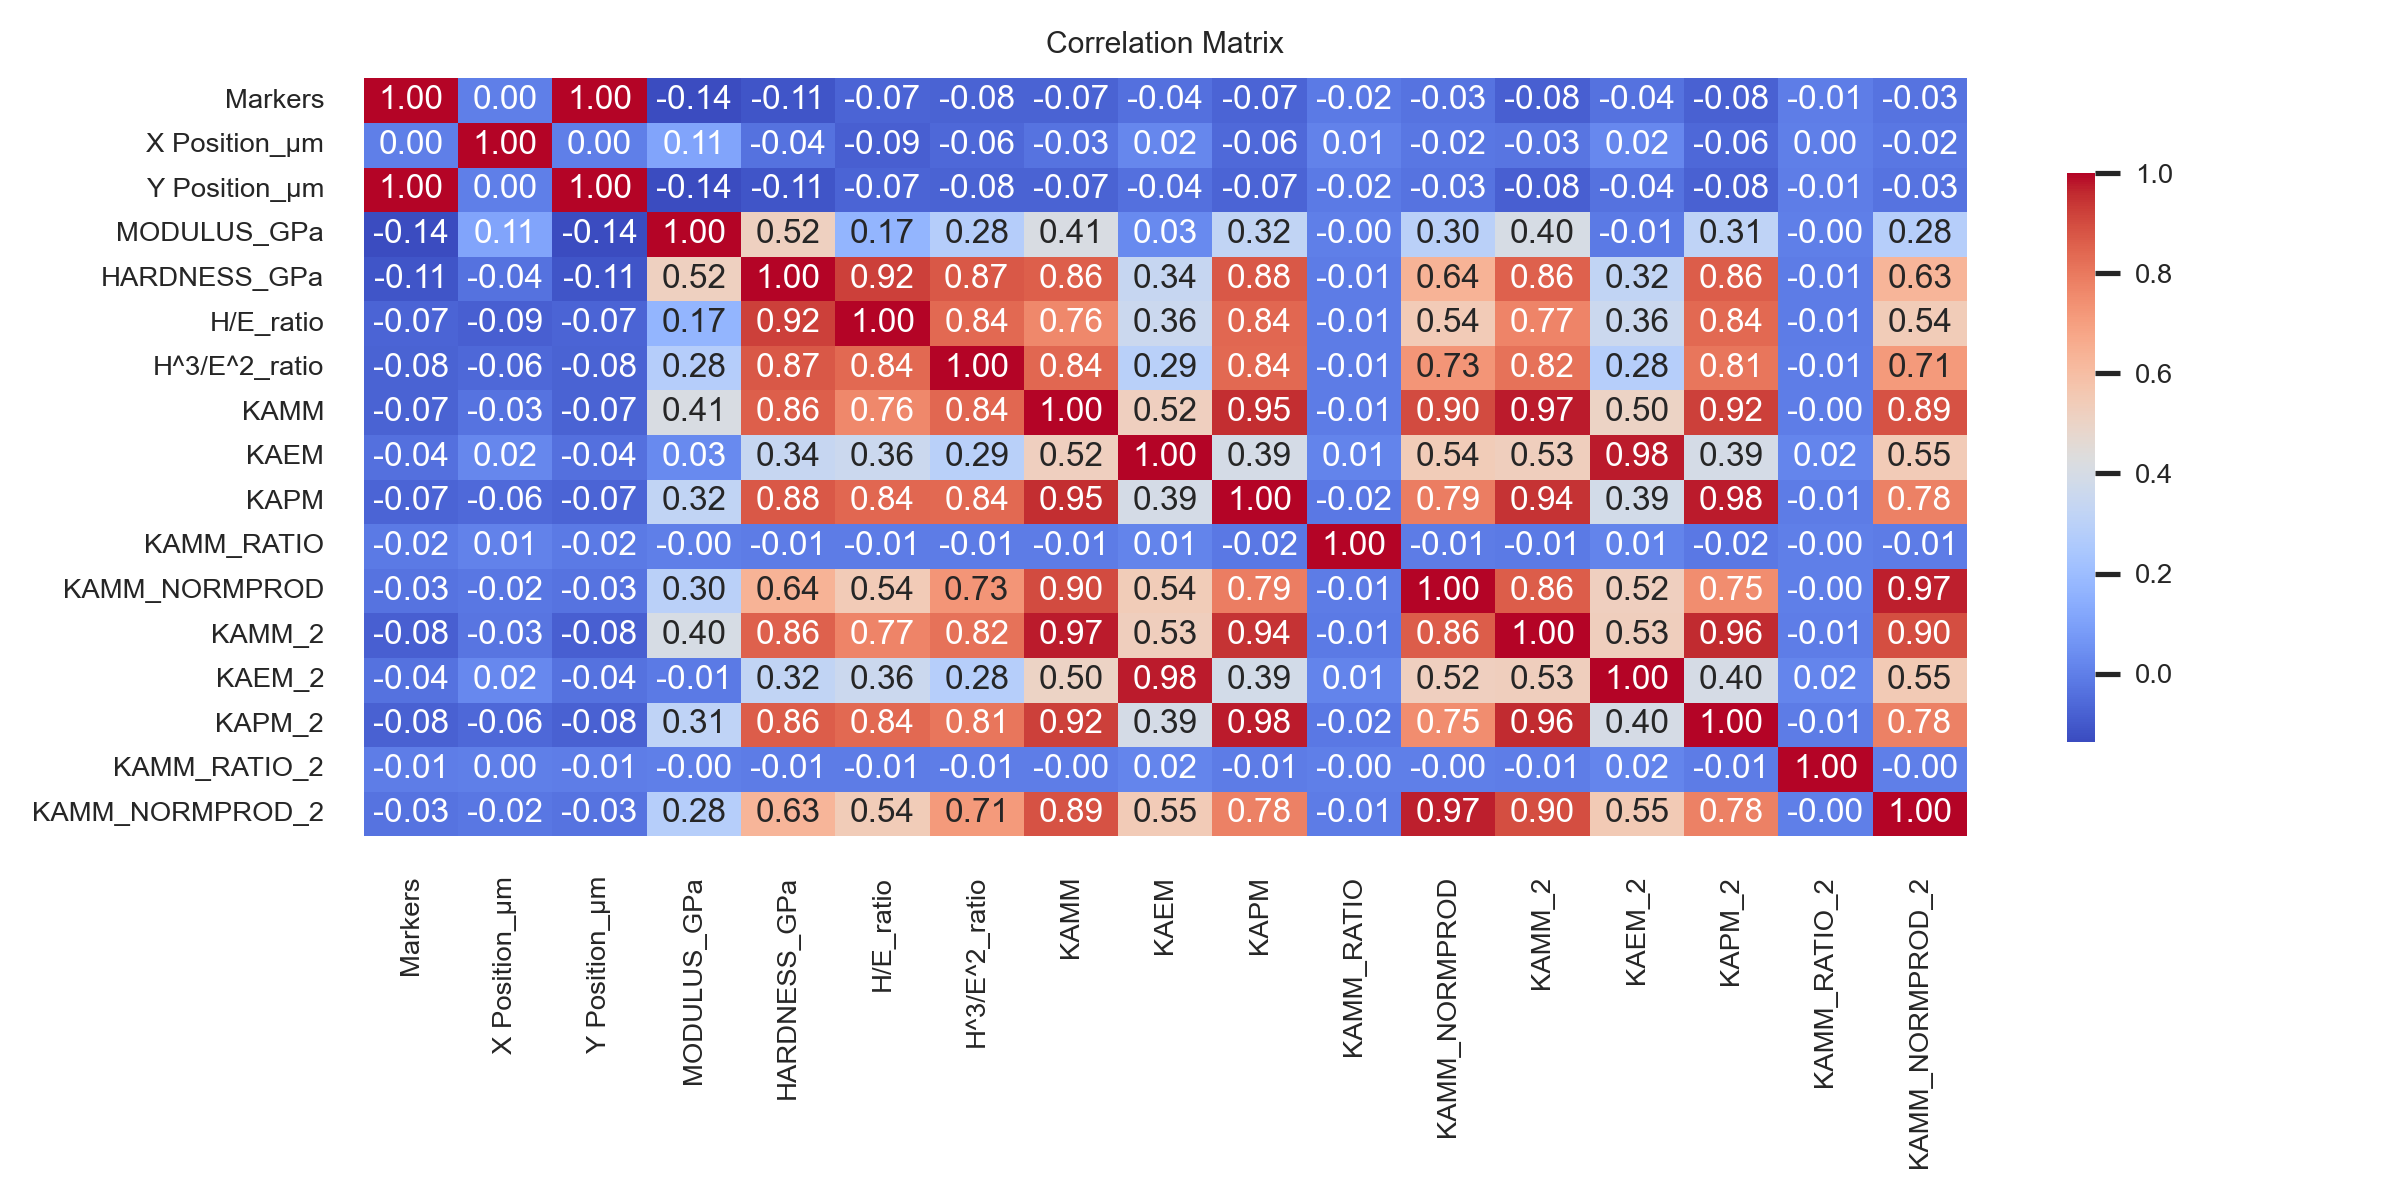
\includegraphics[width=0.95\textwidth]{pictures/CorrMatrix.png}
    \caption{
        Correlation matrix for all mechanical features extracted from the Ni-SiC specimen~\cite{mercier_microstructural_2019}.
    }
    \label{fig:CorrMatrix}
\end{figure}

For the clustering analysis, four algorithms (DBSCAN, Agglomerative Clustering, GMM, and KMeans) were applied under identical preprocessing conditions (z-score normalization and a fixed number of three clusters, following \cite{mercier_microstructural_2019}).  
Three feature spaces of increasing complexity were considered:

\begin{itemize}
    \item \textbf{Case~1 :} \(H\), \(E\), \(H/E\), \(H^3/E^2\);
    \item \textbf{Case~2 :} Case~1 features augmented with first-order KAMM descriptors;
    \item \textbf{Case~3 :} Case~2 features augmented with first and second order KAMM variants.
\end{itemize}

\begin{table}[htbp]
    \centering
    \caption{Maximum feature--feature correlation for each feature set (identical across all clustering algorithms).}
    \label{tab:max_corr_cases}
    \begin{tabular}{lcc}
        \hline
        \textbf{Case} & \textbf{Feature Set Description} & \textbf{Maximum Correlated Pair} \\
        \hline
        Case 1 & Mechanical features (\(H, E, H/E, H^3/E^2\)) 
               & \(H\) -- \(H/E\) \\[2pt]
        Case 2 & All features (\(H, E, H/E, H^3/E^2\) + KAMM descriptors, 1st order only) 
               & KAMM -- KAPM \\[2pt]
        Case 3 & All features (\(H, E, H/E, H^3/E^2\) + KAMM descriptors, incl. higher-order terms) 
               & KAPM -- KAPM\(_2\) \\
        \hline
    \end{tabular}
\end{table}

Because several descriptors are algebraically or physically related, increasing feature-space complexity may introduce redundancy. In supervised learning, strong inter-feature correlation is often undesirable due to multicollinearity and overfitting risks. However, in unsupervised clustering, correlated features are not inherently detrimental. If the correlation reflects meaningful physical coupling (e.g., spatial coherence or phase continuity), redundant descriptors may reinforce cluster compactness and separability. Nevertheless, high correlation can still influence distance metrics, density estimation, or covariance conditioning depending on the algorithm. For this reason, the maximum feature--feature correlation within each feature set is reported in Table~\ref{tab:max_corr_cases} to document potential redundancy and interpret algorithm-dependent behavior.

\subsubsection{Influence of feature sets on clustering}
\label{sec:nisiC_feature_sets}

For visualization, the hardness and elastic-modulus values shown in the clustering maps of Figs.~\ref{fig:1_Agglo_1}--\ref{fig:3_Agglo_2} are normalized by their respective maximum values, $H/H_{\max}$ and $E/E_{\max}$. These dimensionless normalized quantities are used only for visualization and should be distinguished from the z-score standardization applied to the feature matrix before clustering and from the absolute mechanical properties reported in Table~\ref{tab:ref_cluster_feature_comparison} in GPa.

Using the three feature sets defined above (Cases~1--3), clustering results are compared in terms of internal statistical validity, spatial coherence, and phase-wise recovery of mechanical properties. Representative results are shown in Figs.~\ref{fig:1_Agglo_1}, \ref{fig:1_KMEANS_2}, \ref{fig:2_KMEANS_1}, \ref{fig:2_Agglo_2}, \ref{fig:3_GMM_1}, and~\ref{fig:3_Agglo_2}. For consistency, all visualizations follow a standardized four-panel layout: (a) normalized hardness kernel density estimation (KDE) with cluster-wise contributions; (b) spatial phase map; (c) clustered normalized hardness--elastic modulus scatter plot; and (d) normalized elastic-modulus KDE with cluster-wise contributions. Figures~1 correspond to Case~1 (mechanical features only), Figures~2 to Case~2 (mechanical features augmented with first-order KAMM descriptors), and Figures~3 to Case~3 (full feature set including higher-order KAMM descriptors). Colors are used solely to distinguish clusters within each figure; they do not imply a fixed labeling or direct correspondence to a specific physical phase across different algorithms or feature sets.

\paragraph{Case~1: Mechanical features only (\(H, E, H/E, H^3/E^2\))}

Table~\ref{tab:case1_scores} reports the internal clustering validity metrics obtained using only intrinsic mechanical descriptors. KMeans and Agglomerative Clustering yield clearly positive Silhouette values (0.21 and 0.31, respectively), indicating meaningful separation in feature space. Agglomerative Clustering achieves the best overall performance, combining the highest Silhouette score (0.31), the largest Calinski--Harabasz index (1134.53), and the lowest Davies--Bouldin value (1.43), thus reflecting well-separated and compact clusters. KMeans also performs satisfactorily, though with slightly reduced compactness (Davies--Bouldin = 1.86). In contrast, GMM produces weakly separated clusters (Silhouette = 0.05) and a high Davies--Bouldin index (6.74), indicating strong overlap. DBSCAN yields a negative Silhouette score (-0.38), suggesting poor partitioning despite a moderate Calinski value.

Importantly, higher internal validity scores correspond here to improved physical interpretability of the segmentation. As illustrated in Figs.~\ref{fig:1_Agglo_1} and~\ref{fig:1_KMEANS_2}, Agglomerative Clustering produces a spatially coherent three-phase partition that closely matches the expected Ni--SiC microstructure, clearly distinguishing a Ni-rich matrix, SiC-rich particles, and an intermediate interphase. KMeans identifies the same phases but with reduced spatial coherence, while GMM and DBSCAN generate fragmented or poorly localized regions.

These results indicate that mechanical contrast alone can enable phase discrimination; however, successful recovery of physically meaningful regions strongly depends on the algorithm’s ability to generate compact and well-separated structures in feature space.

\begin{table}[htbp]
    \centering
    \caption{Clustering metrics for Case~1 (mechanical feature set \(H, E, H/E, H^3/E^2\))}
    \label{tab:case1_scores}
    \begin{tabular}{lccc}
        \hline
        \textbf{Method} & \textbf{Silhouette} & \textbf{Calinski} & \textbf{Davies} \\
        \hline
        KMeans                   & 0.21 & 802.90  & 1.86 \\
        GMM                      & 0.05 & 102.99  & 6.74 \\
        Agglomerative Clustering & 0.31 & 1134.53 & 1.43 \\
        DBSCAN                  & -0.38 & 76.86 & 2.02 \\
        \hline
    \end{tabular}
\end{table}

\begin{figure}[htbp]
    \centering
    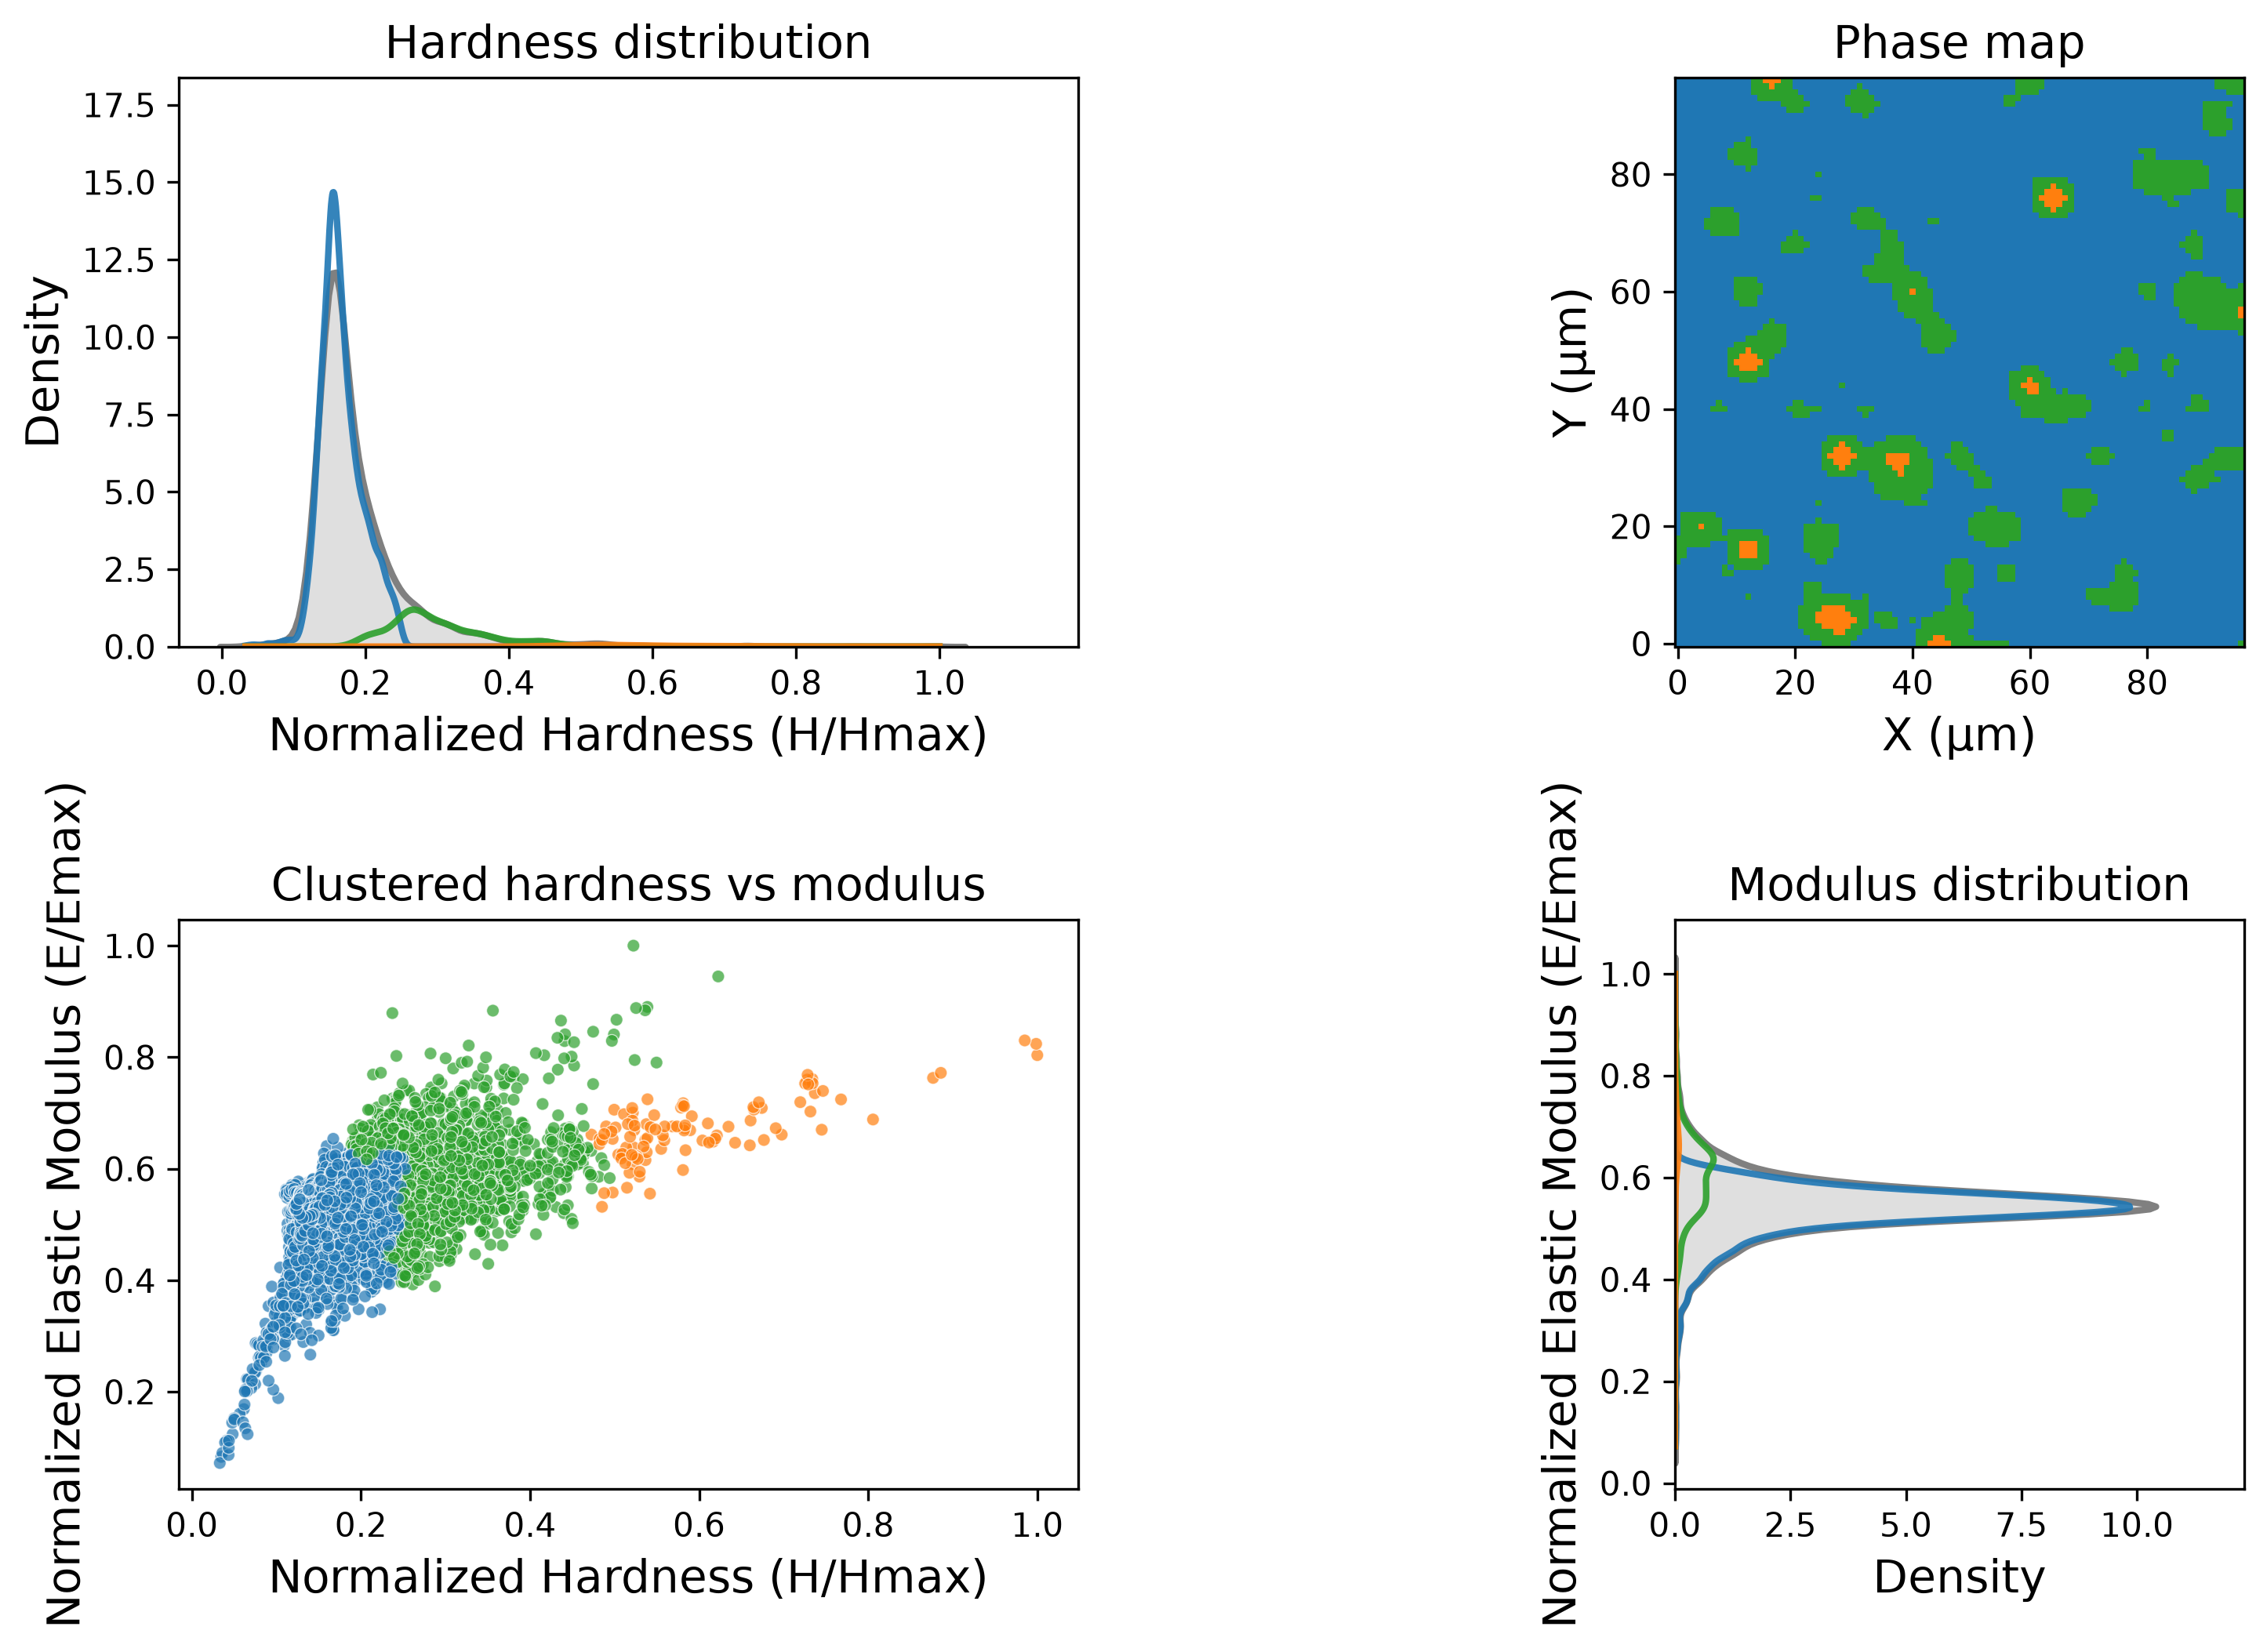
\includegraphics[width=0.95\textwidth]{pictures/1_Agglo_1.png}
    \caption{Agglomerative results using mechanical features only.}
    \label{fig:1_Agglo_1}
\end{figure}

\begin{figure}[htbp]
    \centering
    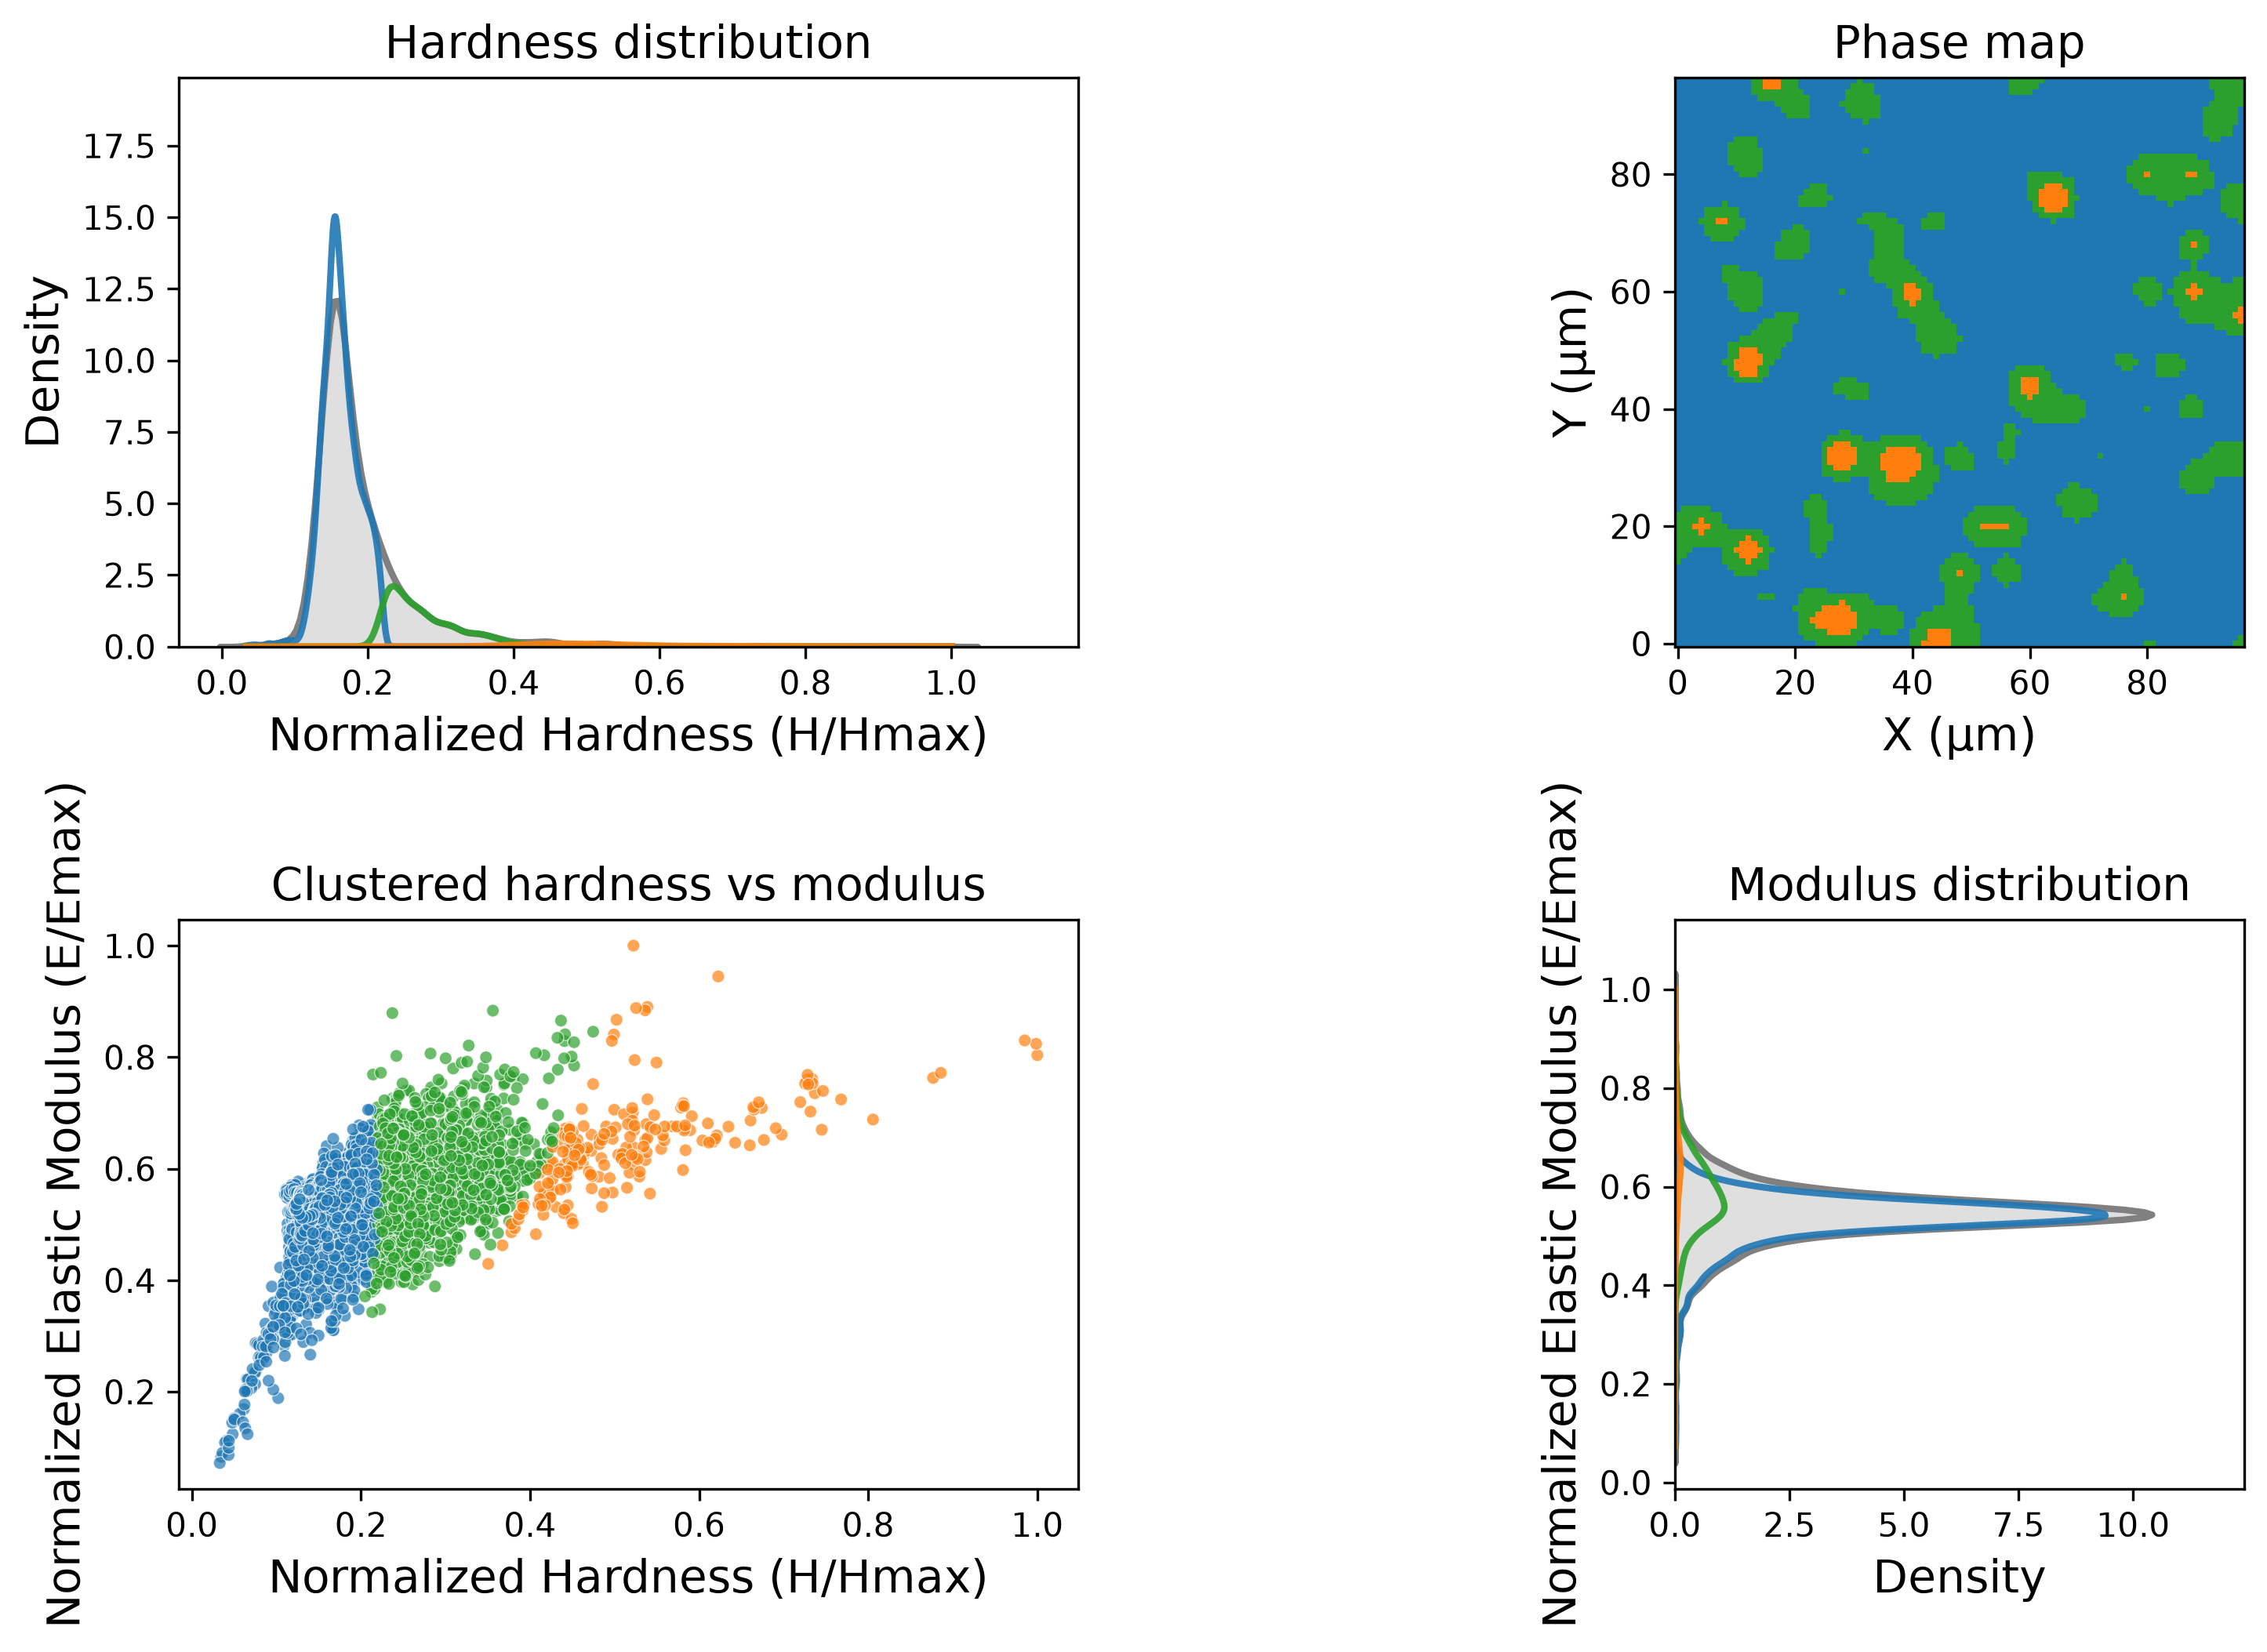
\includegraphics[width=0.95\textwidth]{pictures/1_KMEANS_2.png}
    \caption{KMeans results using mechanical features only.}
    \label{fig:1_KMEANS_2}
\end{figure}

\paragraph{Case~2: Mechanical features with first-order KAMM}
When first-order KAMM descriptors are added, cluster separability decreases compared to Case~1 (Table~\ref{tab:case2_scores}). The silhouette score drops to 0.17 for KMeans and 0.08 for Agglomerative Clustering, while GMM yields a very low value (0.02) and DBSCAN becomes strongly negative (-0.35). Calinski-Harabasz indices also decrease substantially relative to Case~1, and Davies-Bouldin values increase for most methods, indicating reduced compactness and stronger cluster overlap in the augmented feature space. This behavior reflects the strong correlations introduced by the spatial gradient fields, which blur Euclidean distances when KAMM-based descriptors are combined with mechanical ratios.

Despite the reduction in classical clustering metrics, spatial segmentation improves. As shown in Figs.~\ref{fig:2_KMEANS_1} and~\ref{fig:2_Agglo_2}, both KMeans and Agglomerative Clustering reveal a clearer spatial separation between the Ni-rich matrix and the SiC-rich particles. The phase-averaged properties in Table~\ref{tab:ref_cluster_feature_comparison} further show that the mean hardness and modulus of the Ni-like and SiC-like phases are recovered more accurately than in Case~1, with values closer to the corresponding reference data. Thus, first-order KAMM enhances physical interpretability by incorporating spatial gradient information that reflects local mechanical heterogeneity and interfacial transitions around inclusions. Although this additional structure reduces classical clustering metrics based on Euclidean compactness, it improves phase-wise property recovery and spatial coherence of the segmentation.

\begin{table}[htbp]
    \centering
    \caption{Clustering metrics for Case~2 (all mechanical + KAMM features)}
    \label{tab:case2_scores}
    \begin{tabular}{lccc}
        \hline
        \textbf{Method} & \textbf{Silhouette} & \textbf{Calinski} & \textbf{Davies} \\
        \hline
        KMeans                   & 0.17  & 16.10 & 1.76 \\
        GMM                      & 0.02  & 9.27  & 3.91 \\
        Agglomerative Clustering & 0.08  & 15.21 & 2.21 \\
        DBSCAN                   & -0.35 & 15.89 & 1.69 \\
        \hline
    \end{tabular}
\end{table}

\begin{figure}[htbp]
    \centering
    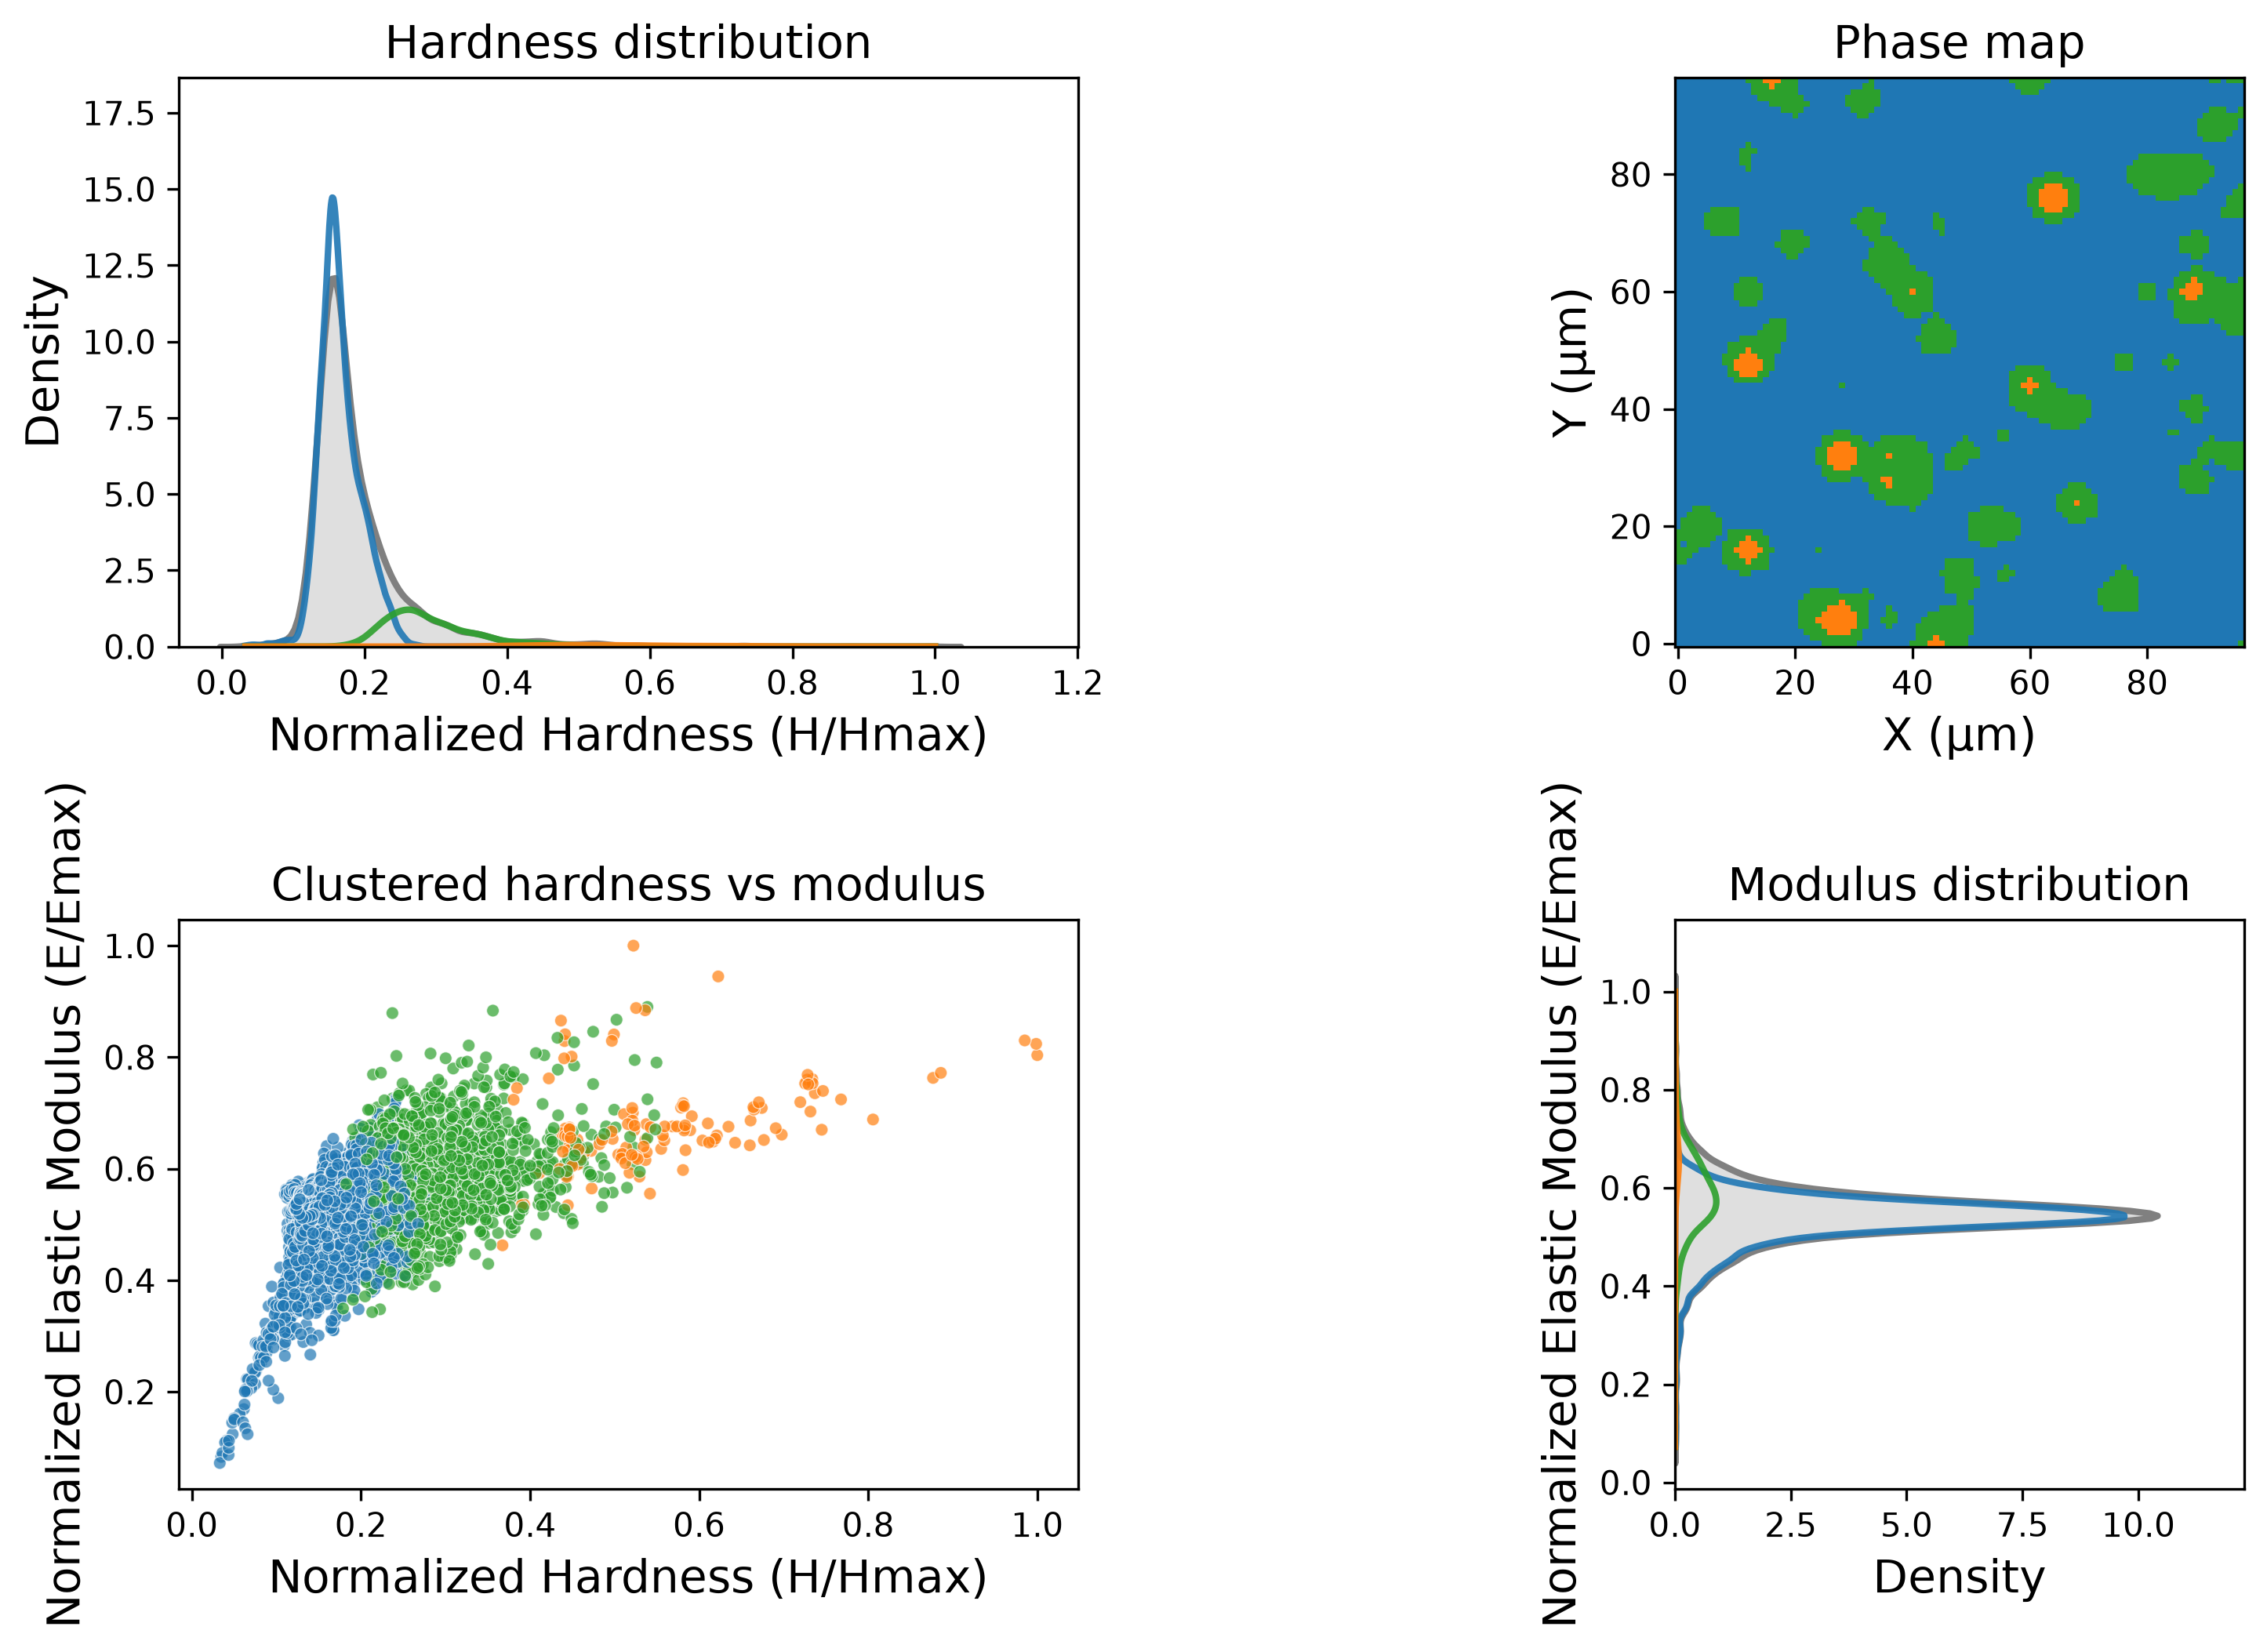
\includegraphics[width=0.95\textwidth]{pictures/2_KMEANS_1.png}
    \caption{KMeans results using mechanical features and first-order KAMM.}
    \label{fig:2_KMEANS_1}
\end{figure}

\begin{figure}[htbp]
    \centering
    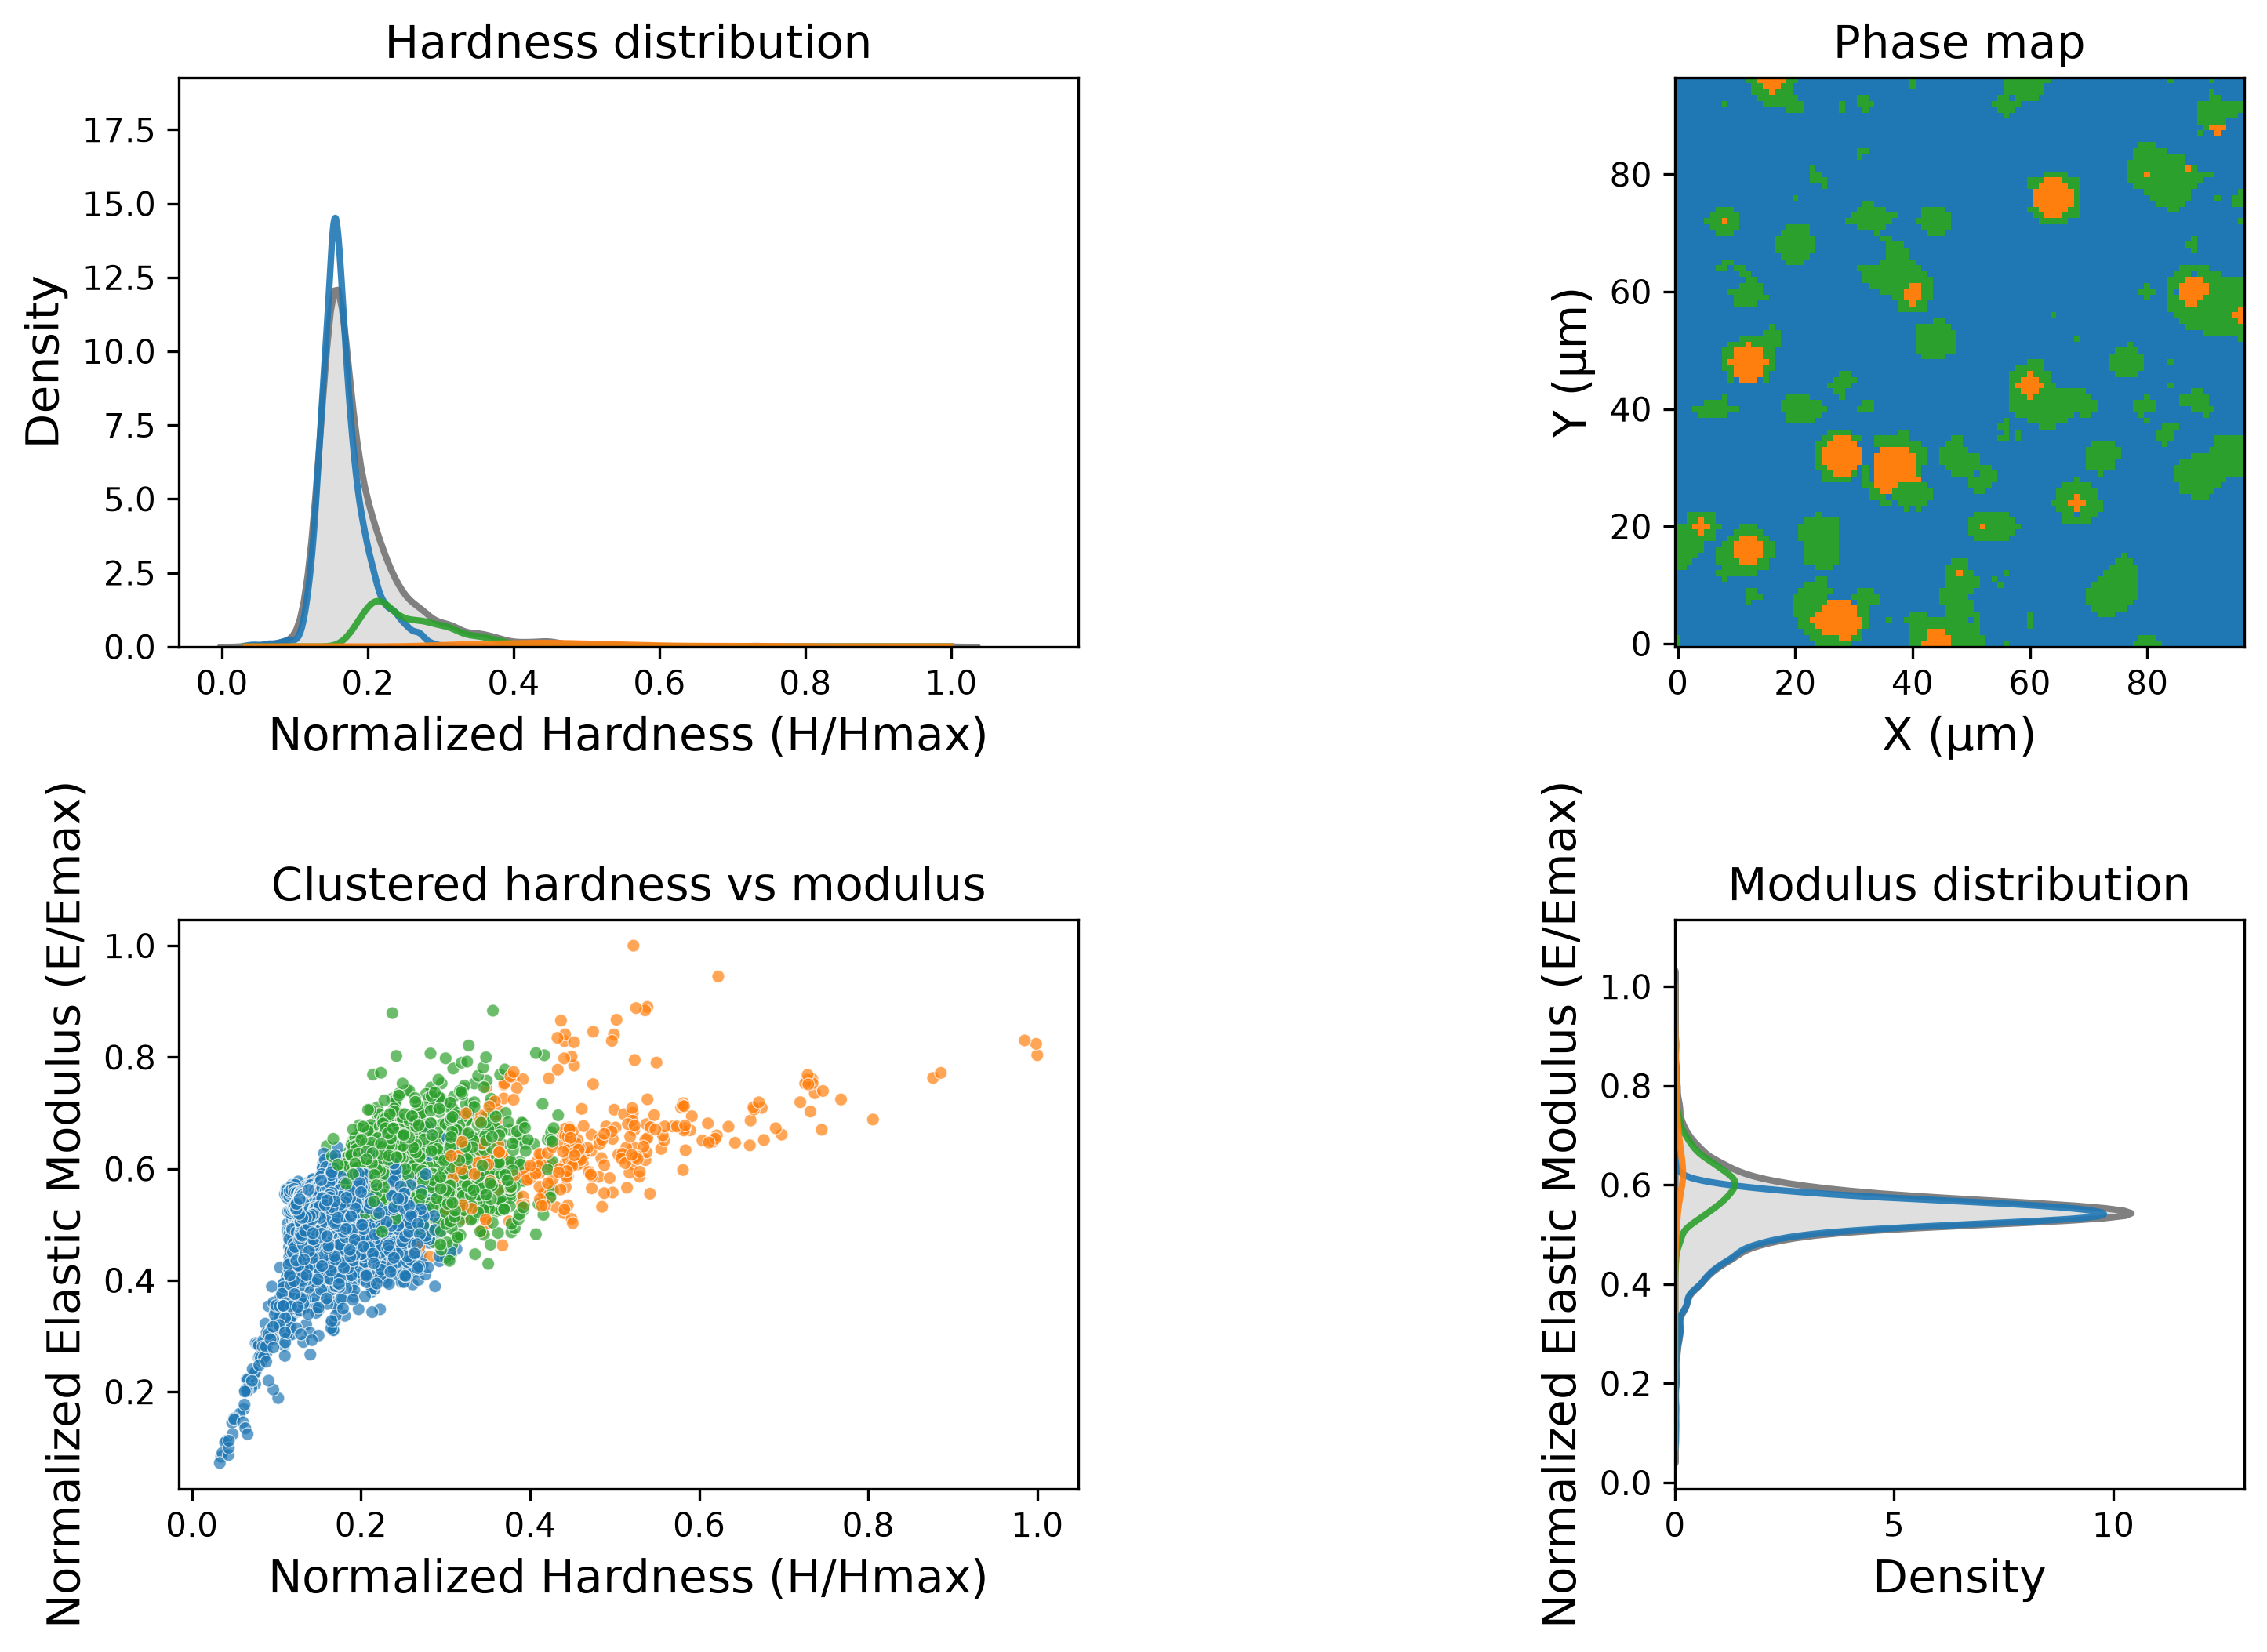
\includegraphics[width=0.95\textwidth]{pictures/2_Agglo_2.png}
    \caption{Agglomerative Clustering results using mechanical features and first-order KAMM.}
    \label{fig:2_Agglo_2}
\end{figure}

\paragraph{Case~3: Full feature set with higher-order KAMM}

Including higher-order KAMM descriptors further modifies the structure of the feature space (Table~\ref{tab:case3_scores}). In contrast to Case~2, the centroid-based methods retain positive Silhouette values, with GMM achieving the highest value (0.19), followed by Agglomerative Clustering (0.15) and KMeans (0.07). However, the Calinski--Harabasz and Davies--Bouldin indices reveal mixed behavior: while GMM shows the largest between-cluster dispersion (Calinski = 58.44), it also exhibits a very high Davies--Bouldin value (10.47), indicating strong cluster overlap. Agglomerative Clustering yields the lowest Davies--Bouldin index (1.99), suggesting comparatively better compactness, though with limited overall separation (Calinski = 6.22). DBSCAN remains unstable, with a negative Silhouette value (-0.33), consistent with fragmented or noisy partitions despite a relatively moderate Davies--Bouldin score.

The phase maps (Figs.~\ref{fig:3_GMM_1} and~\ref{fig:3_Agglo_2}) remain spatially structured; however, the phase-averaged mechanical properties (Table~\ref{tab:ref_cluster_feature_comparison}) tend to shift toward intermediate values. This behavior indicates a form of over-parameterization: the higher-order KAMM descriptors introduce additional variance that reduces the effective contrast between Ni-rich and SiC-rich regions. In practice, these higher-order terms emphasize fine-scale mechanical heterogeneity rather than clear phase separation.

\begin{table}[htbp]
    \centering
    \caption{Clustering metrics for Case~3 (full feature set with higher-order KAMM)}
    \label{tab:case3_scores}
    \begin{tabular}{lccc}
        \hline
        \textbf{Method} & \textbf{Silhouette} & \textbf{Calinski} & \textbf{Davies} \\
        \hline
        KMeans                   & 0.07  & 9.51  & 2.11 \\
        GMM                      & 0.19  & 58.44 & 10.47 \\
        Agglomerative Clustering & 0.15  & 6.22  & 1.99 \\
        DBSCAN                   & -0.33 & 4.14  & 1.75 \\
        \hline
    \end{tabular}
\end{table}

\begin{figure}[htbp]
    \centering
    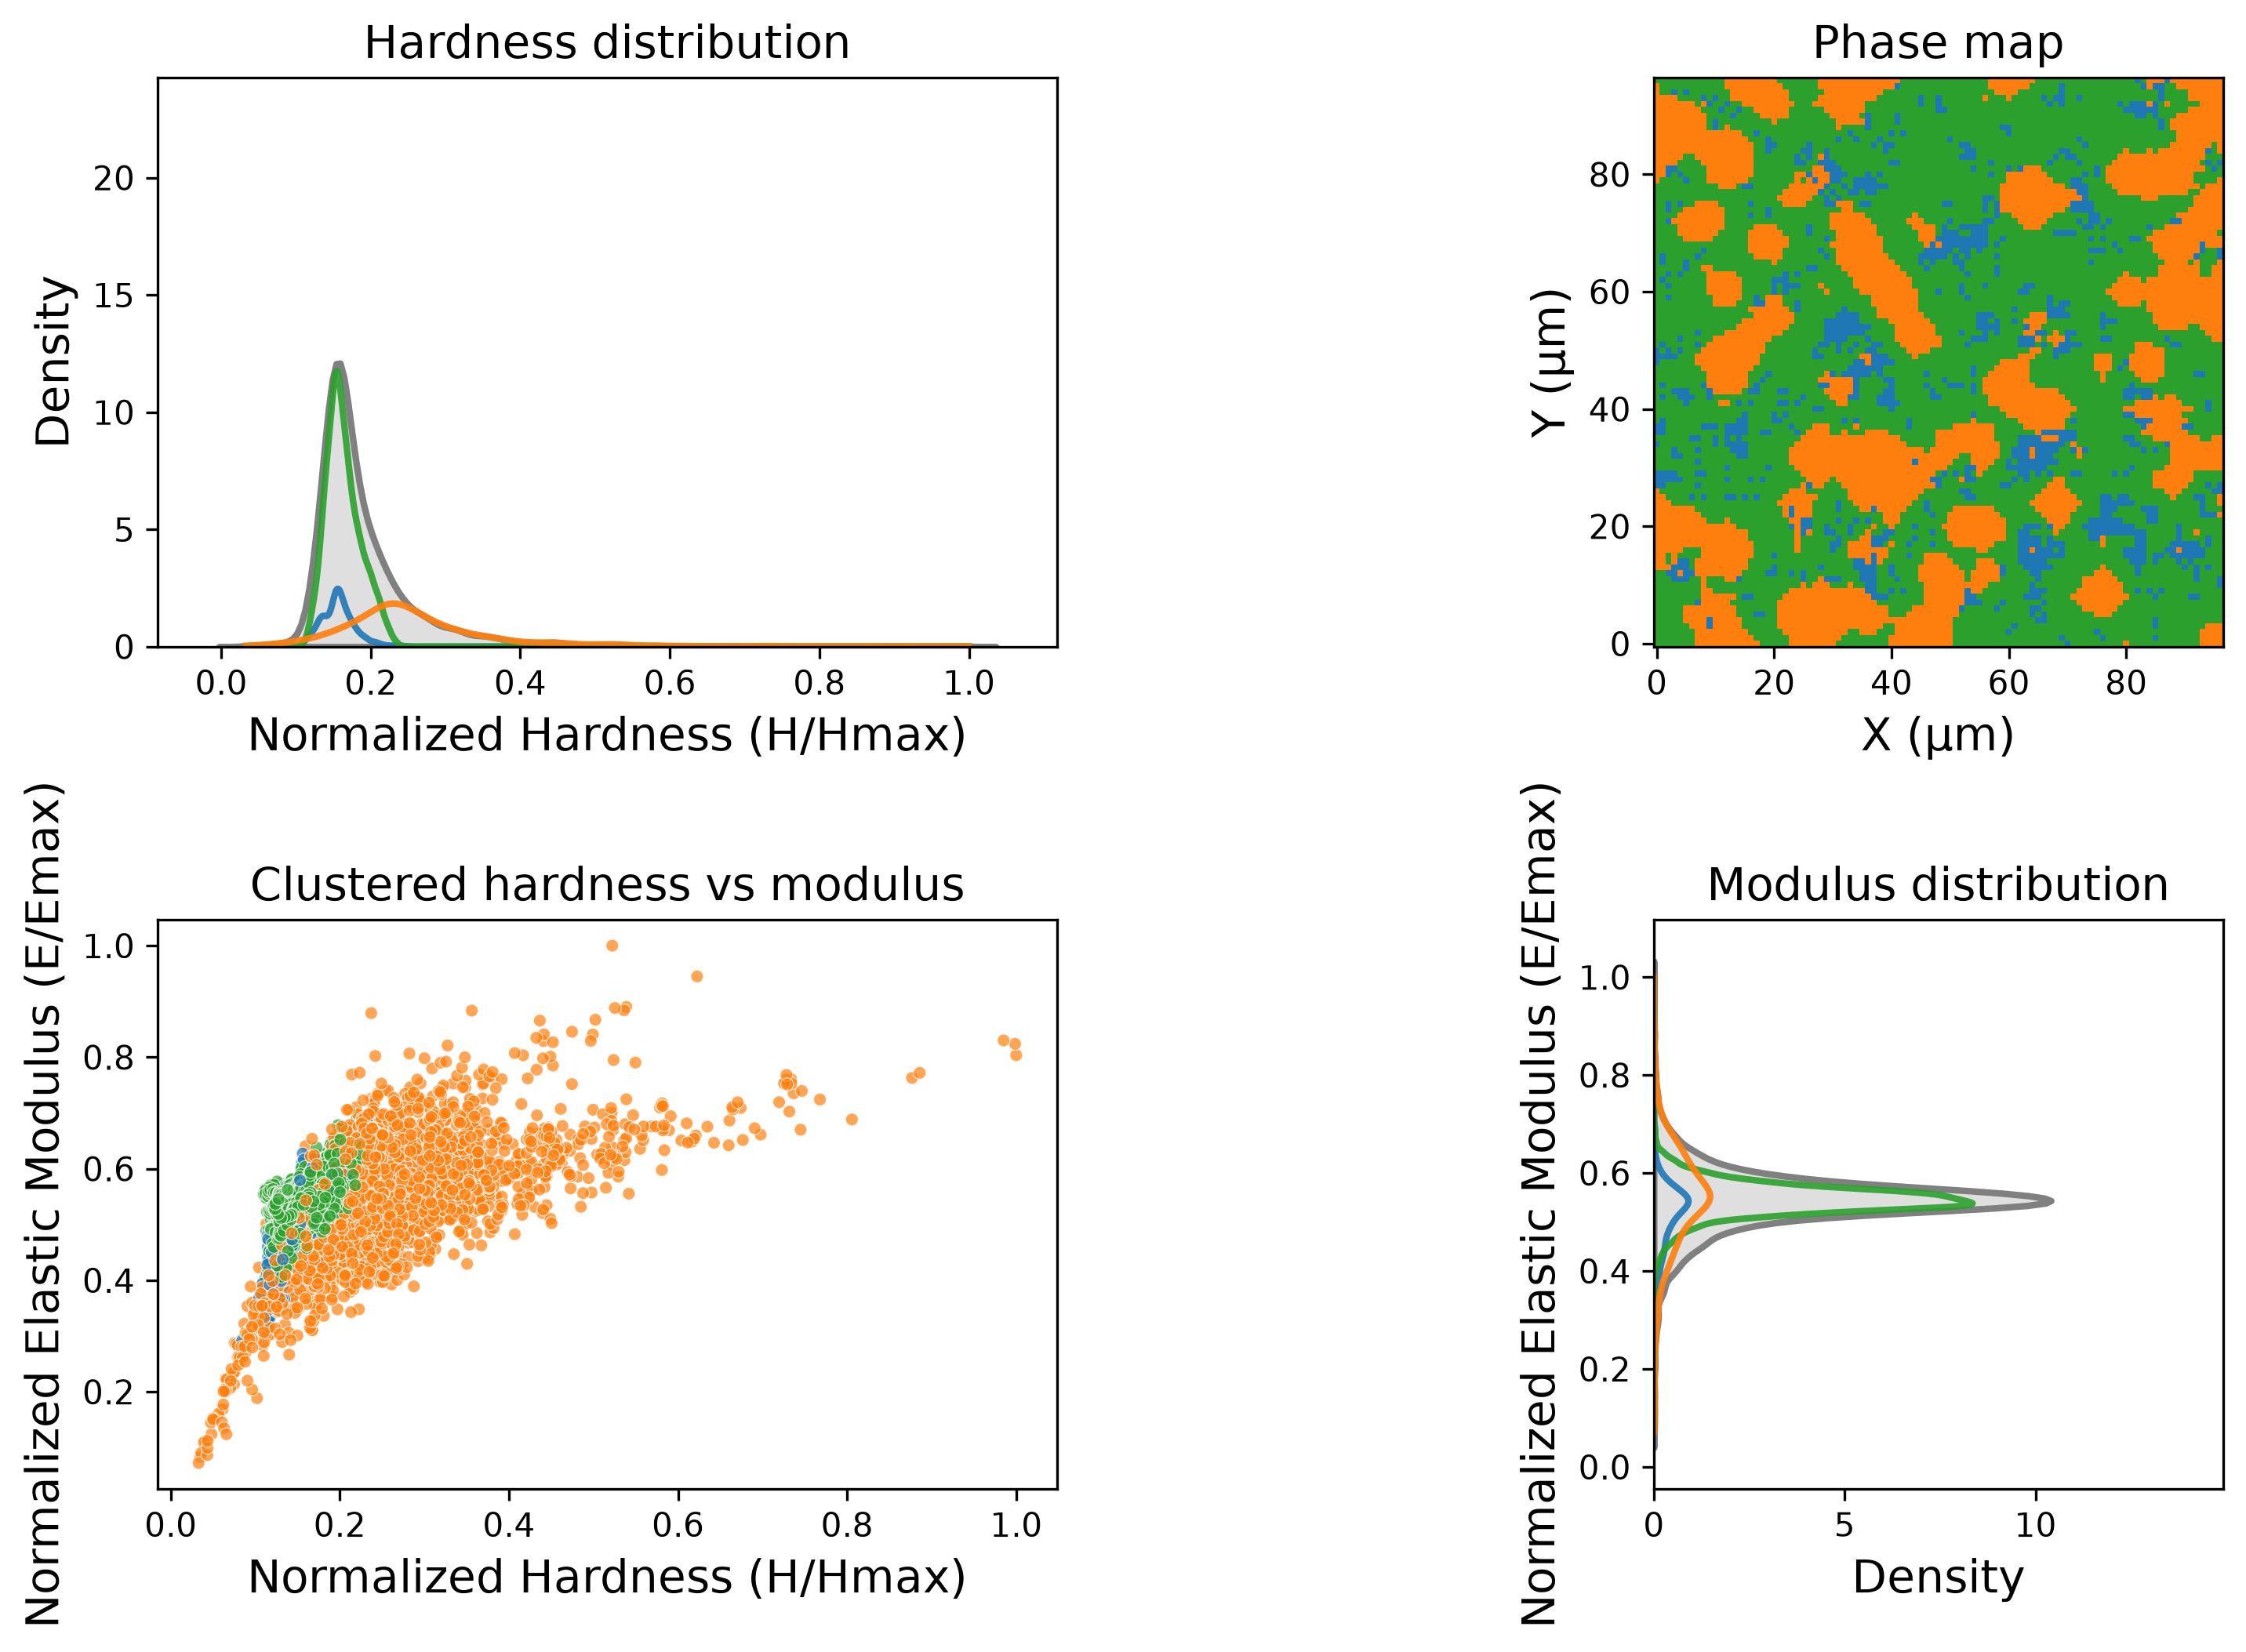
\includegraphics[width=0.95\textwidth]{pictures/3_GMM_1.png}
    \caption{GMM results using the full feature set including higher-order KAMM descriptors.}
    \label{fig:3_GMM_1}
\end{figure}

\begin{figure}[htbp]
    \centering
    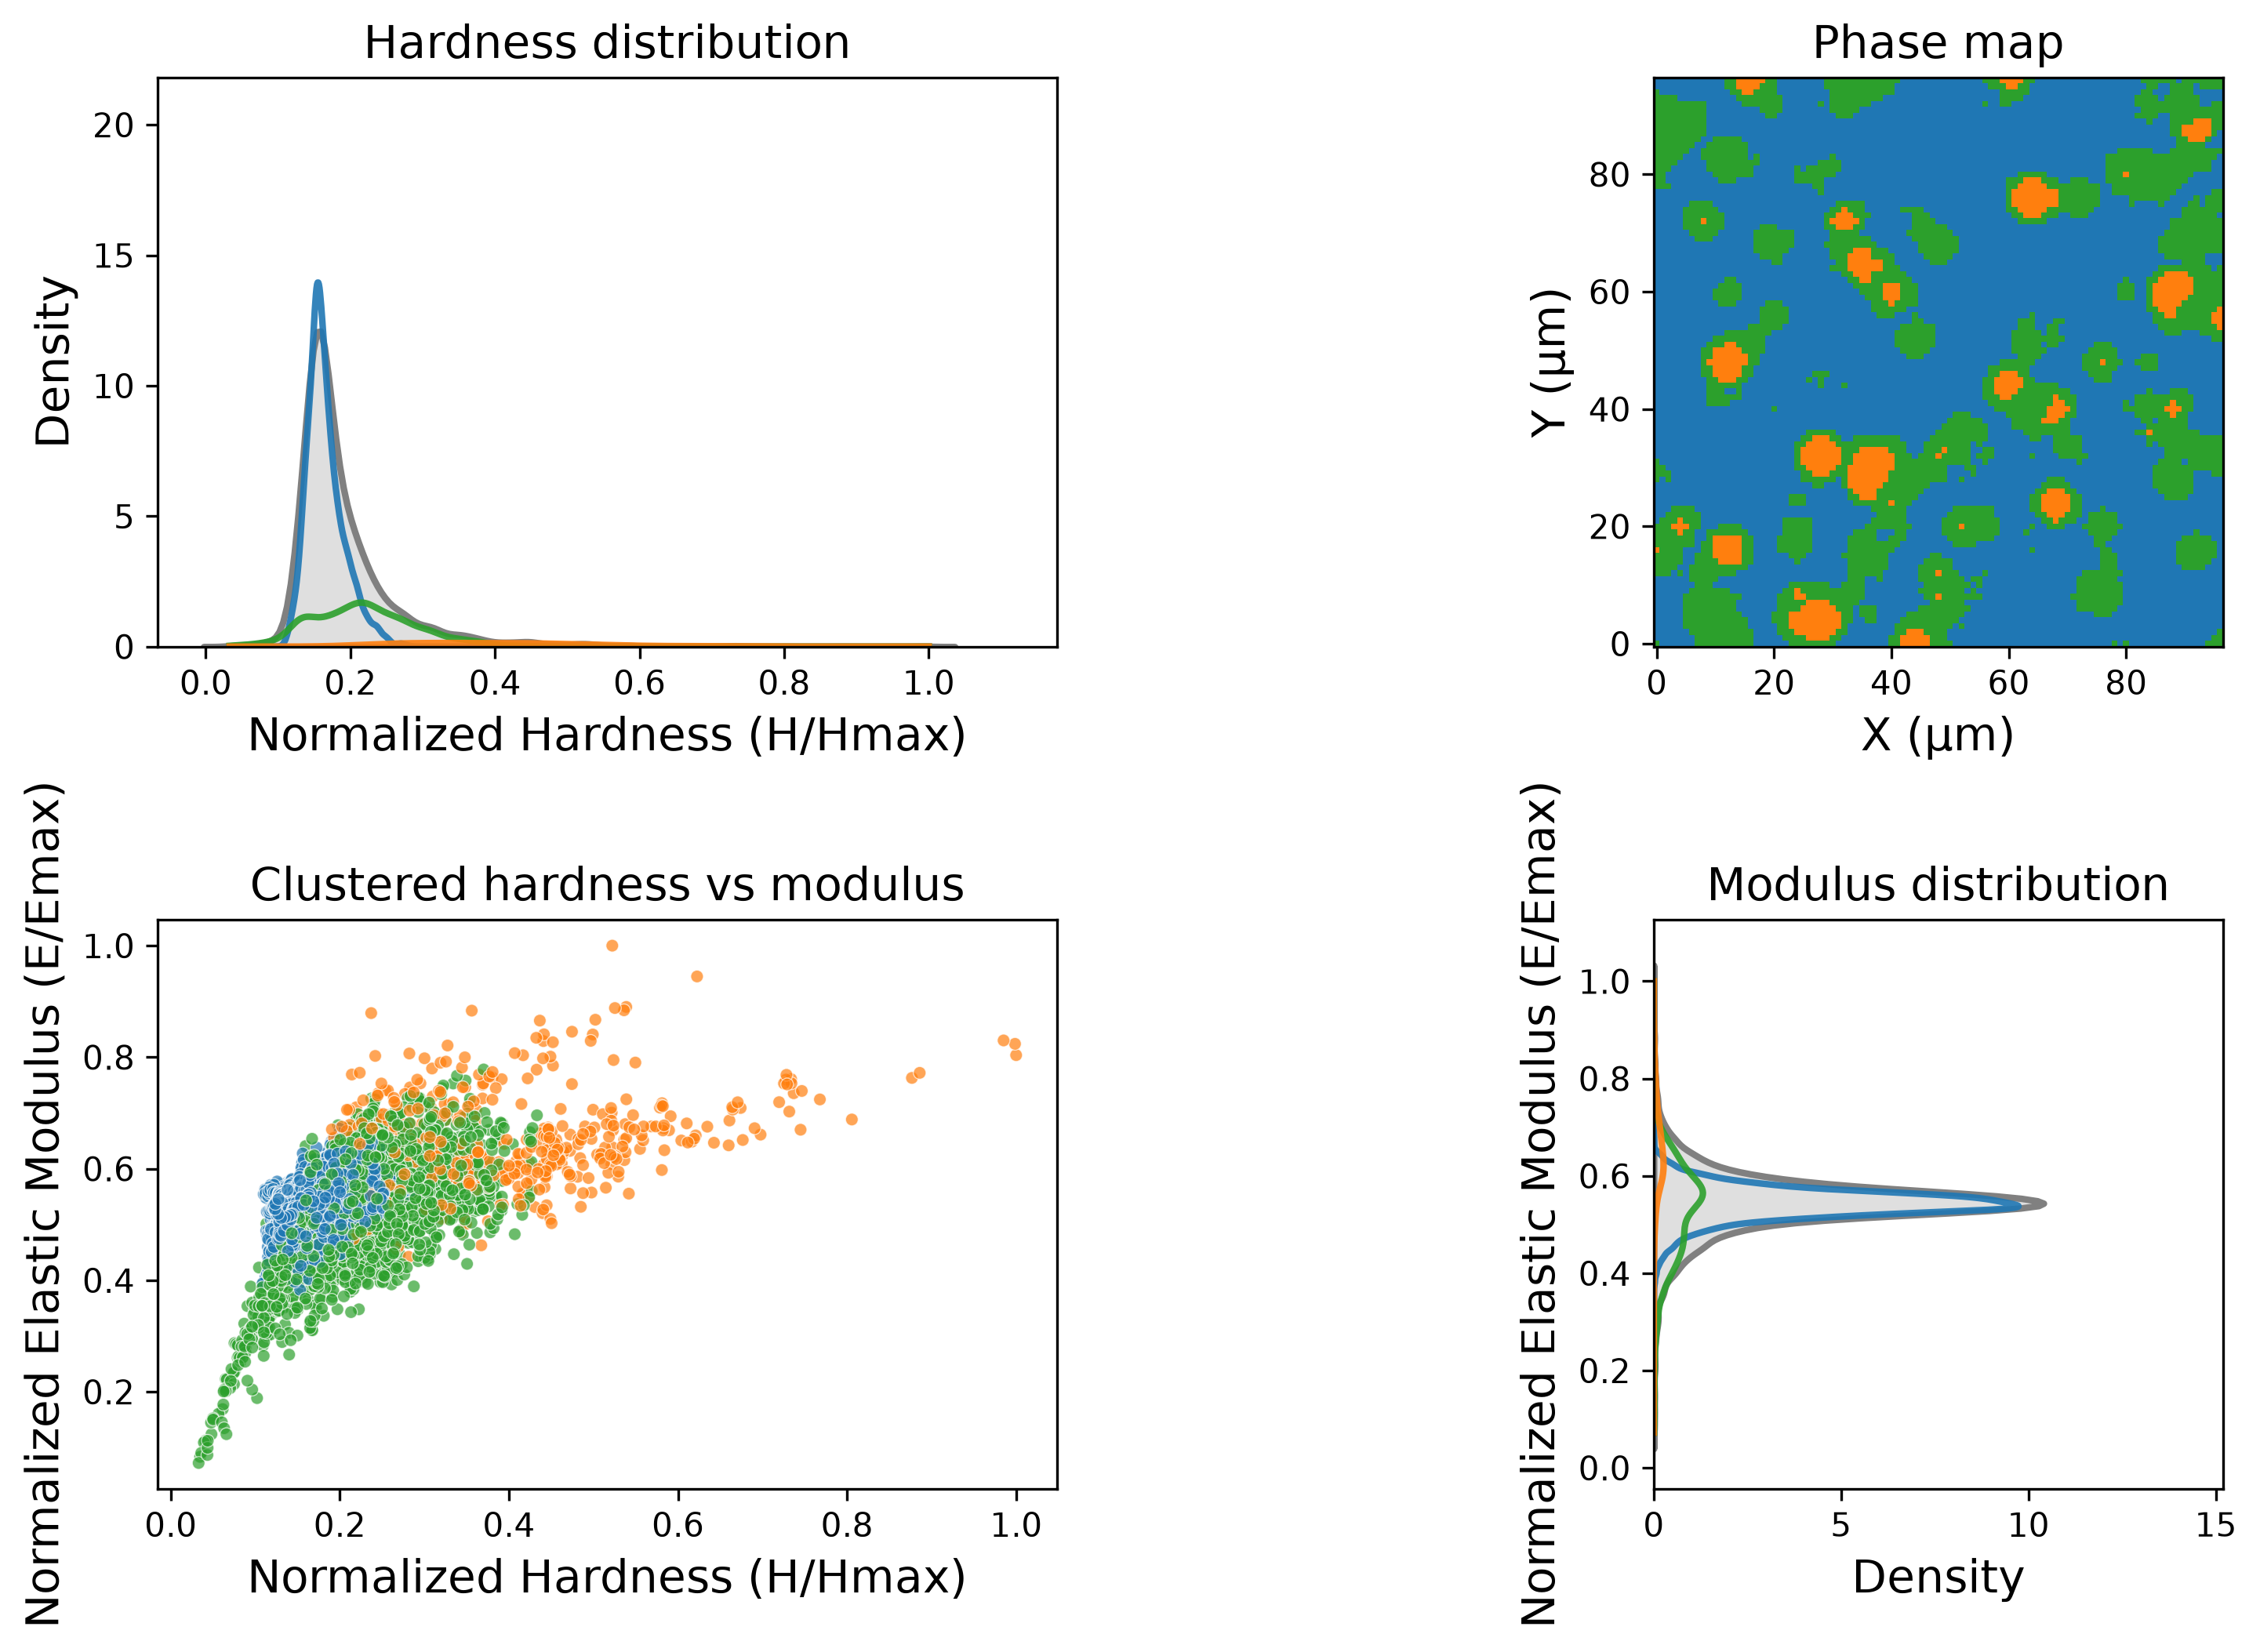
\includegraphics[width=0.95\textwidth]{pictures/3_Agglo_2.png}
    \caption{Agglomerative Clustering results using the full feature set including higher-order KAMM descriptors.}
    \label{fig:3_Agglo_2}
\end{figure}

Overall, a consistent hierarchy emerges across the three cases when comparing the phase-averaged properties in Table~\ref{tab:ref_cluster_feature_comparison}. Mechanical features alone (Case~1) already allow a clear separation between the Ni-like (Phase~1) and SiC-like (Phase~3) clusters, with Phase~1 moduli close to the Ni reference value (219.7~GPa) and Phase~3 exhibiting significantly higher stiffness. The addition of first-order KAMM (Case~2) maintains this contrast while slightly improving spatial coherence, without drastically altering the mean phase properties.

In contrast, the inclusion of higher-order KAMM descriptors (Case~3) leads to a redistribution of mechanical contrast. As shown in Table~\ref{tab:ref_cluster_feature_comparison}, the GMM solution produces intermediate hardness and modulus values for Phase~3 (7.99~GPa, 223.00~GPa), substantially closer to the Ni-like phase than to the $\alpha$-SiC reference (343.2~GPa). This indicates that higher-order spatial descriptors partially blur the mechanical distinction between phases. Although Agglomerative Clustering in Case~3 preserves a larger hardness contrast (15.30~GPa for Phase~3), the associated modulus remains far below the $\alpha$-SiC reference value, confirming that the additional descriptors primarily capture local heterogeneity rather than global phase contrast.

These trends confirm that mechanical features are sufficient to recover the dominant phases, while first-order KAMM improves interphase delineation through spatial gradient information. Higher-order KAMM descriptors, however, mainly encode localized deformation patterns and should therefore be used selectively when the objective extends beyond phase identification toward fine-scale heterogeneity analysis.

Finally, the elastic modulus values—particularly within the SiC-like clusters—remain influenced by outliers associated with unusually high measured stiffness on certain particles. As reflected by the large standard deviations in Table~\ref{tab:ref_cluster_feature_comparison} (e.g., 43.42~GPa for Phase~3 in Case~3 using GMM), these extreme values broaden the cluster distributions and may artificially increase or destabilize the apparent modulus of the hard phase. This sensitivity to noise is consistent with the synthetic benchmark analysis, where added variability similarly broadened property distributions and reduced cluster compactness.

\begin{table}[htbp]
\centering
\caption{Comparison between reference phases and clustered phases (absolute values). Phase~1 corresponds to the lowest mechanical properties (Ni-like), and Phase~3 to the highest mechanical properties ($\alpha$-SiC-like). Values are reported as mean $\pm$ standard deviation.}
\label{tab:ref_cluster_feature_comparison}
\begin{tabular}{l l l c c c c}
\hline
\textbf{Case / Features} & \textbf{Phase} & \textbf{Method} &
\textbf{Hardness (GPa)} & \textbf{Std (GPa)} &
\textbf{Modulus (GPa)} & \textbf{Std (GPa)} \\
\hline

\multicolumn{7}{l}{\textbf{References}} \\
Ni \cite{mercier_microstructural_2019}             & -- & -- & 3.90 & 0.30 & 219.70 & 7.20 \\
$\alpha$-SiC \cite{mercier_microstructural_2019}   & -- & -- & 11.70 & 3.00 & 343.20 & 50.00 \\
\hline

\multicolumn{7}{l}{\textbf{Case 1: $H, E, H/E, H^3/E^2$}} \\
& Phase 1 & Agglo  & 5.30 & 0.95 & 216.88 & 23.64 \\
& Phase 3 & Agglo  & 18.95 & 3.64 & 274.82 & 22.77 \\
& Phase 1 & KMeans & 5.17 & 0.81 & 217.05 & 24.17 \\
& Phase 3 & KMeans & 16.53 & 3.62 & 264.11 & 35.22 \\
\hline

\multicolumn{7}{l}{\textbf{Case 2: $H, E, H/E, H^3/E^2$ + KAMM (1st order)}} \\
& Phase 1 & KMeans & 5.27 & 0.96 & 217.41 & 23.80 \\
& Phase 3 & KMeans & 16.93 & 4.26 & 278.89 & 35.61 \\
& Phase 1 & Agglomerative & 5.14 & 0.81 & 217.07 & 24.64 \\
& Phase 3 & Agglomerative & 14.92 & 3.92 & 264.96 & 35.30 \\
\hline

\multicolumn{7}{l}{\textbf{Case 3: Full feature set + higher-order KAMM}} \\
& Phase 1 & GMM    & 4.95 & 0.68 & 211.72 & 23.38 \\
& Phase 3 & GMM    & 7.99 & 3.32 & 223.00 & 43.42 \\
& Phase 1 & Agglomerative & 5.29 & 0.83 & 222.19 & 15.28 \\
& Phase 3 & Agglomerative & 15.30 & 4.44 & 266.16 & 35.05 \\
\hline

\end{tabular}
\end{table}

\section{Conclusion}
\label{sec:conclusion}

The objective of the study was to assess the value of a simple neighborhood-informed descriptor for nanomechanical phase mapping rather than to develop a new clustering methodology. This work evaluated the use of the neighborhood-informed descriptor \textit{Kernel-Averaged Mechanical Mismatch} (KAMM), adapted from established EBSD neighborhood metrics, for nanomechanical property mapping and phase identification. The main findings can be summarized as follows:

\begin{itemize}
    \item KAMM quantifies local mechanical heterogeneity through neighborhood comparisons in the \((E,H)\) space, thereby incorporating spatial context that is absent from conventional feature sets.
    
    \item When integrated into the clustering space, first-order KAMM can improve phase recovery and spatial interpretability for selected algorithm--dataset combinations, although the benefit is not systematic.
    
    \item The effectiveness of KAMM is algorithm- and condition-dependent. Improvements are observed for selected centroid-, linkage-, and distribution-based configurations, whereas limited benefits or degraded performance are observed under noisy conditions and for density-based clustering.
    
    \item Conventional clustering metrics do not always reflect physical relevance. Improvements in spatial coherence and phase identification can occur even when statistical separability indices decrease, highlighting the need for complementary evaluation criteria based on microstructural consistency.
    
    \item KAMM highlights regions of strong local mechanical heterogeneity, including phase boundaries and graded transitions. In the experimental dataset, these regions may exhibit intermediate mechanical responses, although their physical or measurement-related origin cannot be established without independent correlative validation.
    
    \item Practical implementation requires careful feature selection to limit redundancy and preserve clustering stability, for instance by restricting to lower-order descriptors or removing strongly correlated features.
\end{itemize}

Future work will focus on:
\begin{itemize}
    \item Extending the synthetic generator to three-dimensional microstructures and incorporating mixed indentation responses close to phase boundaries.
    \item Extending the synthetic framework to non-Gaussian and empirically derived intra-phase property distributions.
    \item Improving robustness under challenging experimental conditions (noise, non-uniform sampling, measurement artefacts),
    \item Exploring advanced clustering strategies (e.g.\ OPTICS, HDBSCAN, graph-based or spatially constrained methods),
    \item Integrating systematic outlier detection and preprocessing pipelines.
\end{itemize}

Overall, KAMM provides a simple and computationally efficient approach to incorporate neighborhood awareness into nanomechanical phase mapping and to improve the reliability of data-driven phase identification.

% ----------------------------------------------------------
% 6. Authors Contributions
% ----------------------------------------------------------
\section*{Author Contributions}

D.~Mercier performed the modelling work and led the manuscript writing.  
Y.~El~Gharoussi developed the synthetic dataset generators and implemented the analysis code.

% ----------------------------------------------------------
% 7. Code and Data Availability
% ----------------------------------------------------------
\section*{Code and Data Availability} The Python code used to generate the synthetic nanomechanical maps, compute the neighborhood-based descriptors, perform clustering, and evaluate clustering performance is provided as Supplementary Material. The supplementary files include the synthetic-data generator and analysis workflow required to reproduce the synthetic benchmark calculations presented in this study.

% ----------------------------------------------------------
% 8. Acknowledgements
% ----------------------------------------------------------
\section*{Acknowledgements}

The authors gratefully acknowledge Davide Di Stefano and Pascal Salzbrenner for rich and insightful discussions that helped shape and refine this work. This research has received support from the NanomeCommons project (Horizon 2020, Grant Agreement No.~952869). The authors are solely responsible for the content presented herein; this does not necessarily reflect the views of the European Union.

% ----------------------------------------------------------
% 9. Declaration of Generative AI and AI-Assisted Technologies in the Manuscript Preparation
% ----------------------------------------------------------
\section*{Declaration of Generative AI and AI-Assisted Technologies in the Manuscript Preparation}

During the preparation of this manuscript, the author(s) used Microsoft Copilot for grammar correction, syntax refinement, and improvements in clarity. After using this tool, the author(s) carefully reviewed and edited the content as needed and take full responsibility for the final version of the published article.

% ----------------------------------------------------------
% 10. References
% ----------------------------------------------------------
\bibliographystyle{unsrt}
\bibliography{references}

\end{document}

